%THIS IS THE MAIN FILE THAT TELLS LATEX WHICH FILES TO INCLUDE IN YOUR THESIS.

%THIS TEMPLATE PASSED DOWN FROM COURTNEY DRESSING
%EDITED SLIGHTLY AND UPLOADED TO OVERLEAF BY BEN COOK (bacook17@gmail.com)

% use "plain" for committee to read, or for printing single-spaced in general
\documentclass[plain]{hvdthesis}

% use "bound" for submitting to Harvard 
%\documentclass[bound]{hvdthesis}

% no more microfilm?
%\documentclass[microfilm]{hvdthesis}

% Put all required packages and setup in one file
%\usepackage{deluxetable}
%\usepackage{bibunits} %% bibunits.sty allows references at the end of each chapter

%\def\hsp{\def\baselinestretch{1.5}\normalsize} % intermediate spacing

\bibpunct{(}{)}{;}{a}{}{,}
\newcommand{\bmath}{\boldmath}
\usepackage{epstopdf}
\usepackage{epsfig}
\usepackage{aasmod}
\usepackage{amsmath}
\usepackage{amssymb}
\usepackage{rotating}
\usepackage{verbatim}
\usepackage{longtable}
\usepackage{lscape}
\usepackage{subfig}
\usepackage{float}
\usepackage{color}
\usepackage{fltpage}
\usepackage{url}
\usepackage{rotating}
\usepackage[innercaption]{sidecap}
\usepackage{pdfpages}
\usepackage{xspace}

%this block is new from Greg S to accommodate change in 2013 format requiring page numbers be centered on every page
\usepackage{fancyhdr}
\pagestyle{fancy}
\fancyhf{}
\lhead{\it{\leftmark}}
\rhead{}
\chead{}
\cfoot{\thepage}
\lfoot{}
\rfoot{} 
\renewcommand{\headrulewidth}{0.0pt}

%\usepackage{apjfonts}

%% makes \subfloat command put (a), (b), ... labels at top of subfigure instead of bottom
\captionsetup[subfigure]{position=top,font=bf,captionskip=0pt,topadjust=0pt,farskip=0pt}

%\pagestyle{headings}
%\pagestyle{myheadings}
% could also have pagestyle{myheadings}
% problem w/ default headings is that they're
% a bit too wide for the page (the chapter titles are too long!)


% Put all your useful macros, shortcuts, and commands in one file
\newcommand{\ksmag}{\emph{Ks}~magnitudes }
\newcommand{\jmag}{\emph{J}~magnitudes }
\newcommand{\kpmags}{\emph{Kp}~magnitudes }
\newcommand{\kpmag}{\emph{Kp}~magnitude }
\newcommand{\teff}{\ensuremath{T_{\mathrm{eff}}}}                               
\newcommand{\logg}{\ensuremath{\log g}} 
\newcommand{\kepler}{{\em Kepler}\xspace}
\def\msun{{\rm\,M_\odot}}                                                       
\def\rsun{{\rm\,R_\odot}}        
\def\mearth{{\rm\,M_\oplus}}                                                
\def\rearth{{\rm\,R_\oplus}} 
\def\fearth{{\rm\,F_\oplus}} 
\def\lsun{{\rm\,L_\odot}}  
\newcommand{\hho}{H$_2$O}
\newcommand{\hh}{H$_2$}
\newcommand{\oo}{O$_2$}
\newcommand{\chhhh}{CH$_4$}
\newcommand{\mjup}{{\rm M}_{\rm Jup}}
\newcommand{\kms}{\rm km\ s^{-1}}
\newcommand{\mps}{\rm m\ s^{-1}}
\newcommand{\kelvin}{\rm K}
\newcommand{\degr}{\ensuremath{^\circ}}
\newcommand{\angstrom}{\rm \AA}
\newcommand{\oneday}{\rm day}
\newcommand{\days}{\rm days}
\newcommand{\hours}{\rm hours}
\newcommand{\meter}{\rm m}
\newcommand{\HST}{{\it HST}}
\newcommand{\hubble}{{\it HST}}
\newcommand{\spitzer}{{\it Spitzer}}
\newcommand{\zeroth}{$0^{\rm th}$}
\newcommand{\first}{$1^{st}$}
\newcommand{\second}{$2^{nd}$}
\newcommand{\third}{$3^{rd}$}
\newcommand{\fourth}{$4^{th}$}
\newcommand{\e}{${\rm e^{-}}$}
\newcommand{\persecond}{${\rm s^{-1}}$}
\newcommand{\perpixel}{${\rm pixel^{-1}}$}
\newcommand{\divideoot}{{\tt divide-oot}}
\newcommand{\modelramp}{{\tt model-ramp}}
\newcommand{\chisq}{$\chi^2$}
\newcommand{\calwf}{{\tt calwf3}}
\newcommand{\rp}{$R_{p}$}
\newcommand{\rs}{$R_{\star}$}
\newcommand{\flt}{{\tt flt}}
\definecolor{orange}{rgb}{.8,0.4,0}
\newcommand{\question}[1]{\sffamily {\em {\color{orange} [#1]}}\normalfont}
\newcommand{\todo}[1]{\sffamily {\em {\color{orange} #1}}\normalfont}
\newcommand{\edit}[1]{{#1}}
\newcommand{\mad}{\rm MAD}


\newcommand{\outline}[1]{
\todo{\begin{itemize}
#1 
\end{itemize}}}

\usepackage{natbib}
\bibliographystyle{aasjournal}
\usepackage{placeins} %Floatbarrier command
\PassOptionsToPackage{hyphens}{url}
\usepackage[colorlinks=true, allcolors=blue]{hyperref}
\usepackage{amsmath}
\usepackage{subfig}
\usepackage{graphicx}
\usepackage{siunitx}
\usepackage{comment}
\usepackage{svg}
\usepackage[normalem]{ulem}
\usepackage{romannum}
\usepackage{bm} %Bold math symbols
\usepackage{mathtools} %For dcases
\allowdisplaybreaks %To allow long equations to break pages.
\usepackage[T1]{fontenc} %To fix narrow underscores
\usepackage{textcomp} %For 'upquote' in listing
\usepackage{accsupp} %For non-copyable line numbers
\usepackage{nicefrac}
\usepackage{dsfont}

\usepackage{titlesec}
%\titleformat{\section}https://www.overleaf.com/project/60ee83c9e199e57c09f31d5b
%{\color{red}\normalfont\Large\bfseries}
%{\color{red}\thesection}{1em}{}

\newcommand{\sr}[1]{{\bf\color{red} [SR: #1]}}
\newcommand{\suit}{{\it{SUIT}}}
\graphicspath{{./}{Figures/}}

\usepackage{enumitem}

\newlist{abbrv}{itemize}{1}
\setlist[abbrv,1]{label=,labelwidth=1in,align=parleft,itemsep=0.1\baselineskip,leftmargin=!}


\author{Soumya Roy}
\title{Thesis Title Goes Here}
\department{}
\subject{}
\month{Month}
\year{Year}
\advisor{Professor Durgesh Tripathi}

\begin{document}

% include the dissertation acceptance form

\includepdf[pages={1}]{placeholder_dac.pdf}

\clearpage
\thispagestyle{empty}
\begin{center}
\vspace*{\fill}
Page left intentionally blank.
\vspace*{\fill}
\end{center}

\frontmatter

	%% Title page
\makecover
	%% Copyright
%\copyright
	%% Abstract
\justifying

\abstract{

Solar flares are the largest magnetic eruptions in the Solar system. The enigmatic magnetic eruptions have been studied for over a century. However, their complete spectral energy distribution is not yet derived. One of the main missing components is flare energetics in the photosphere and chromosphere. While there are many measurements of flare energetics in the extreme-ultraviolet (EUV), soft and hard X-rays, the measurements in other wavelength bands, especially in the near ultraviolet, are sparse. The Solar Ultraviolet Imaging Telescope ({\it SUIT}) on board Aditya-L1 by the Indian Space Research Organisation (ISRO) aims to fill the gap by observing the flares in the wavelength band 200 {--} 400 nm. Moreover, using the EUV and X-ray observations, there has been great progress in flare physics. However, there is a lack in our understanding of the evolution of thermal and non-thermal energy during the course of the evolution of flares and the partition between the thermal and non-thermal energy, including the conversion mechanism at play. This thesis is in two parts. In one part, we perform the initial preparatory analysis carried out for the {\it SUIT} instrument, including the throughput model, jitter estimation and its effect on imaging, the on-ground spectral and photometric validation, forward modelling of {\it SUIT} observations using the data obtained from realistic MHD simulations from MURaM, and the stellar calibration plan. We also carry out analysis with existing IRIS data in anticipation of SUIT, to comment on the effect of solar flares in the local environment. In the second part, we use the existing EUV and X-ray observations to study the thermal and non-thermal energy in solar flares and demonstrate the importance of volume estimation on the total thermal energy budget and, thereby, the efficiency of the conversion from non-thermal to thermal energy. We propose a triangulation method using existing tools and observations from different vantage points to estimate the volume of emitting plasma in flares as a function of time. Finally, we study two flares which are observed by SUIT in NUV combined with EUV, NUV, Soft and Hard X-ray spectroscopy and for the first time we discuss the flare observations and initial results in this broad wavelength coverage.

}

%\input{abstract_short.tex}
	%% Table of Contents
{\singlespace
\tableofcontents
}
\newpage
\clearpage

	%% List of Figures
%\addcontentsline{toc}{chapter}{List of Figures}
%\listoffigures
%\newpage
	%% List of Tables
%\addcontentsline{toc}{chapter}{List of Tables}
%\listoftables

\newpage
	%% Acknowledgments
%Thank people here.
\thispagestyle{plain}
\addcontentsline{toc}{chapter}{Acknowledgments}
\chaptermark{Acknowledgments}

\vskip 0.5cm
{\centerline {\Large \bf Acknowledgments}}
\vskip 0.5cm
\normalsize
Thank people here.


%\hfill -- RCH
%\newpage

\clearpage
%	%% Dedication
%\input{dedication.tex}
\thispagestyle{plain}
\addcontentsline{toc}{chapter}{Dedication}

\vspace*{\fill}
{\centerline {\em Your thoughtful dedication goes here.}}
%\vskip 1.5cm
%{\centerline {\em }}
\vspace*{\fill}

%\clearpage

\mainmatter
\pagestyle{fancy}


%% Uncomment the next four lines, plus the \begin{bibunit} and \end{bibunit} 
%% to use bibunits.  Read bibunits.dvi for more documentation
%\bibliographyunit[\chapter]
%\bibliographystyle*{apj}
%\bibliography*{apj-jour,planets}
%\bibliographyunit

\chapter[Introduction]{Introduction}\label{c:intro}
\justifying

The Sun is our nearest astrophysical object, which serves as a natural laboratory for various branches of Physics - atomic physics, spectroscopy, turbulence, magneto-hydrodynamics, stellar evolution, dynamo and magnetism and plays a key role in space and terrestrial weather. The Sun is also the primary source of light and energy on earth. So it is only natural that we try to understand the different physical processes involved in the energectics of the Sun, which indirectly affects life on Earth. In this chapter I briefly introduce the Sun and various layers of its atmosphere. At the end we provide a motivation for the thesis.

The Sun is a G2V star, with surface luminosity $3.86~\times~10^{26}$ W and an effective temperature of $\sim 5780~K$. The Sun is mostly made out of Hydrogen(92.1\%) and Helium(7.8\%) along with negligible quantities of heavier elements C, N, O, Mg, Si, Ne and Fe. The study of the Sun can be mainly divided into three components: the Solar interior, the Solar atmosphere and the Heliosphere.

%%%%%%%%%%%%%%%%%%%%%%%%%%%%%%%%%%%%%%%%%%%%%%%%%%%%%%%
\section{The solar interior}\label{solar_int}
%%%%%%%%%%%%%%%%%%%%%%%%%%%%%%%%%%%%%%%%%%%%%%%%%%%%%%%

In the innermost zone of the star the Sun has a temperature of about 15 MK and a density of $1.6~\times~10^{5}~km.m^{-3}$ that fuses Hydrogen into Helium mainly by p-p cycle \citep{bethe38} and to some extent by CNO cycle \citep{bethe39}. 

%% ############# %%
\begin{figure}[h!]
    \centering
    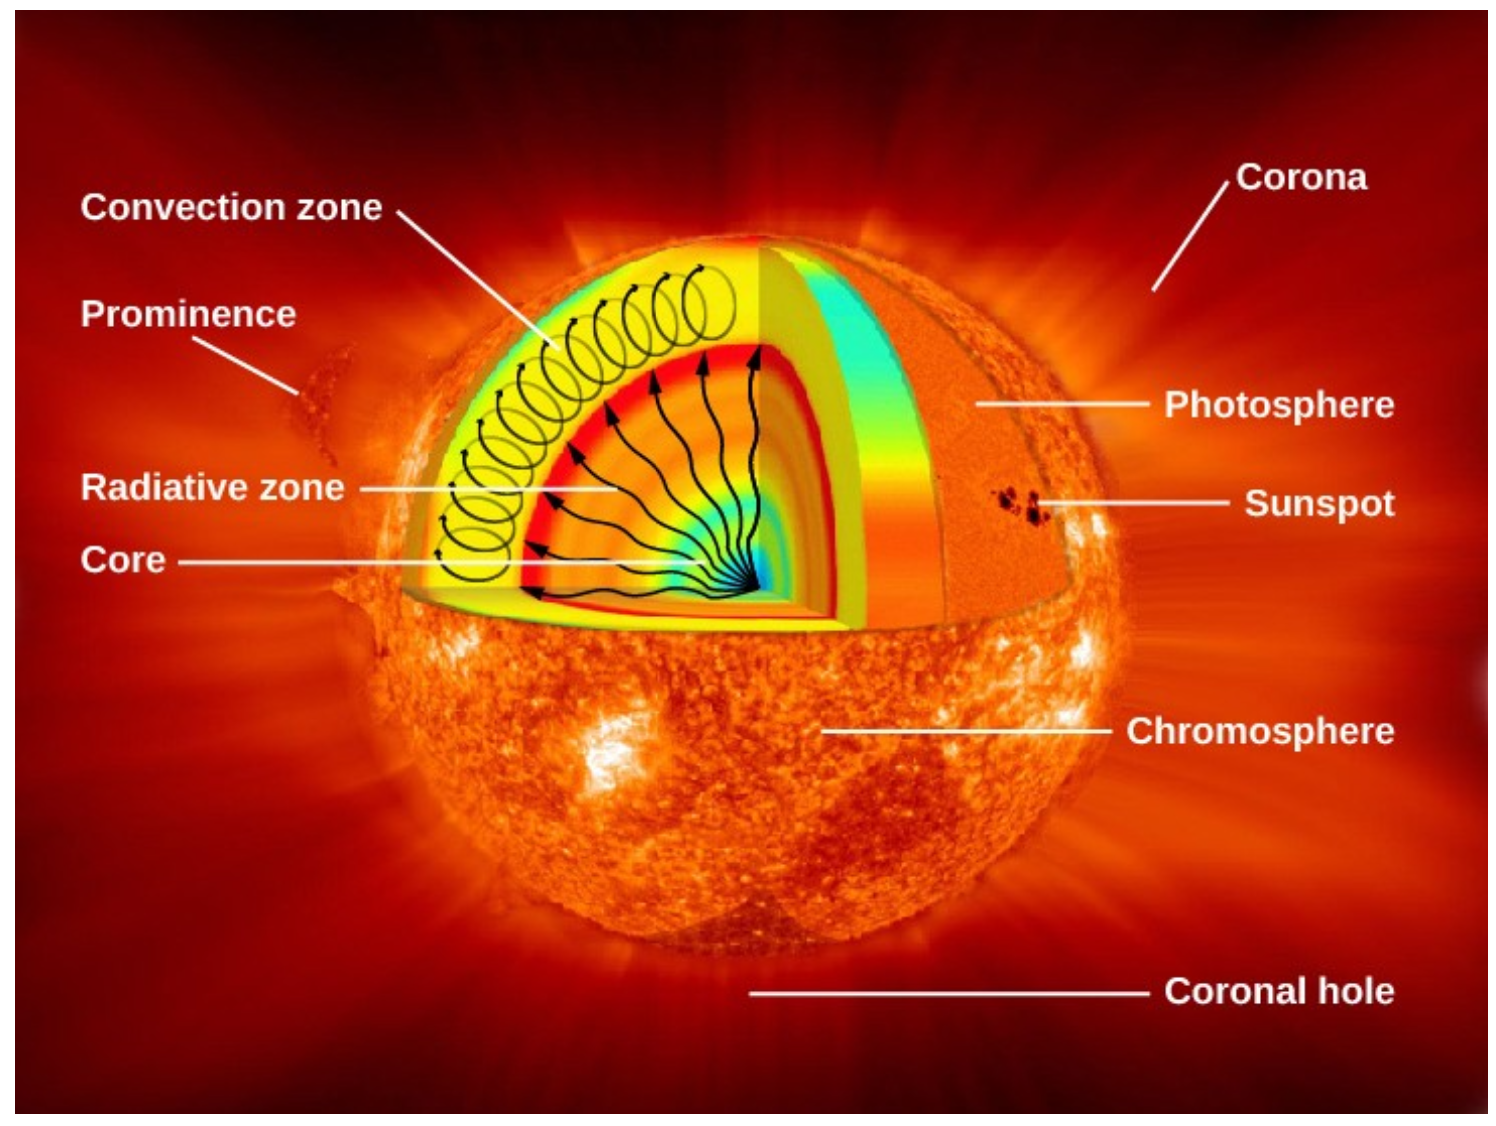
\includegraphics[width = 0.8\linewidth]{Figures/solar_int.png}
    \caption{A schematic depiction of the different layers of the Sun. The figure also shows some of the most prominent magnetic structures on the Sun e.g sunspot, prominence, coronal hole. Credit : NASA/Goddard.}
    \label{fig_solar_int}
\end{figure}
%% ############# %%

Fig.~\ref{fig_solar_int} shows a schematic diagram of various layers of the Sun. Beyond the core we have the optically thick radiative zone, where the Hydrogen and Helium are completely ionized. The high energy $\gamma$-ray photons generated in the core, have very small mean free path in this region, as they collide numerous times eventually thermalizing becoming visible photon. Beyond the radiative zone the degree of ionization of Hydrogen and Helium changes drastically giving rise to a sharp temperature gradient. This is the convective zone where the energy from the inner layers of the Sun is transported adiabetically to the surface of the Sun. In between the radiative and the convective zone, there is a thin layer, roughly at $\sim~0.7~R_{\odot}$ known as the tacholine, which is believed to play a major role in generating Sun's magnetic field via the Dynamo process \citep{corbard01}. 

The core and the radiative zone of the Sun rotates as a solid body, whereas the convective zone rotates differentially. The rotation period varies from $\sim~25~days$ to $\sim~35~days$ from the equator to the pole.

%%%%%%%%%%%%%%%%%%%%%%%%%%%%%%%%%%%%%%%%%%%%%%%%%%%%%%%
\section{The solar atmosphere}\label{solar_atmos}
%%%%%%%%%%%%%%%%%%%%%%%%%%%%%%%%%%%%%%%%%%%%%%%%%%%%%%%

The layers outside the convection zone together, form the solar atmosphere - the Photosphere, which is also known as the Sun's surface, the Chromosphere, the transition region and the Corona. While we can define geometrical height or depths to define these layers, it is much more useful to define them using the local optical depths of various spectral lines, which are directly used to observe the layers. This also gives us a idea about which spectral features originate mainly from which portions of the solar atmosphere. Fig.~\ref{fig_solar_atm} shows the variation of temperature and number density across various layers of the Solar atmosphere \sr{Ref. here}.

%% ############# %%
\begin{figure}[h!]
    \centering
    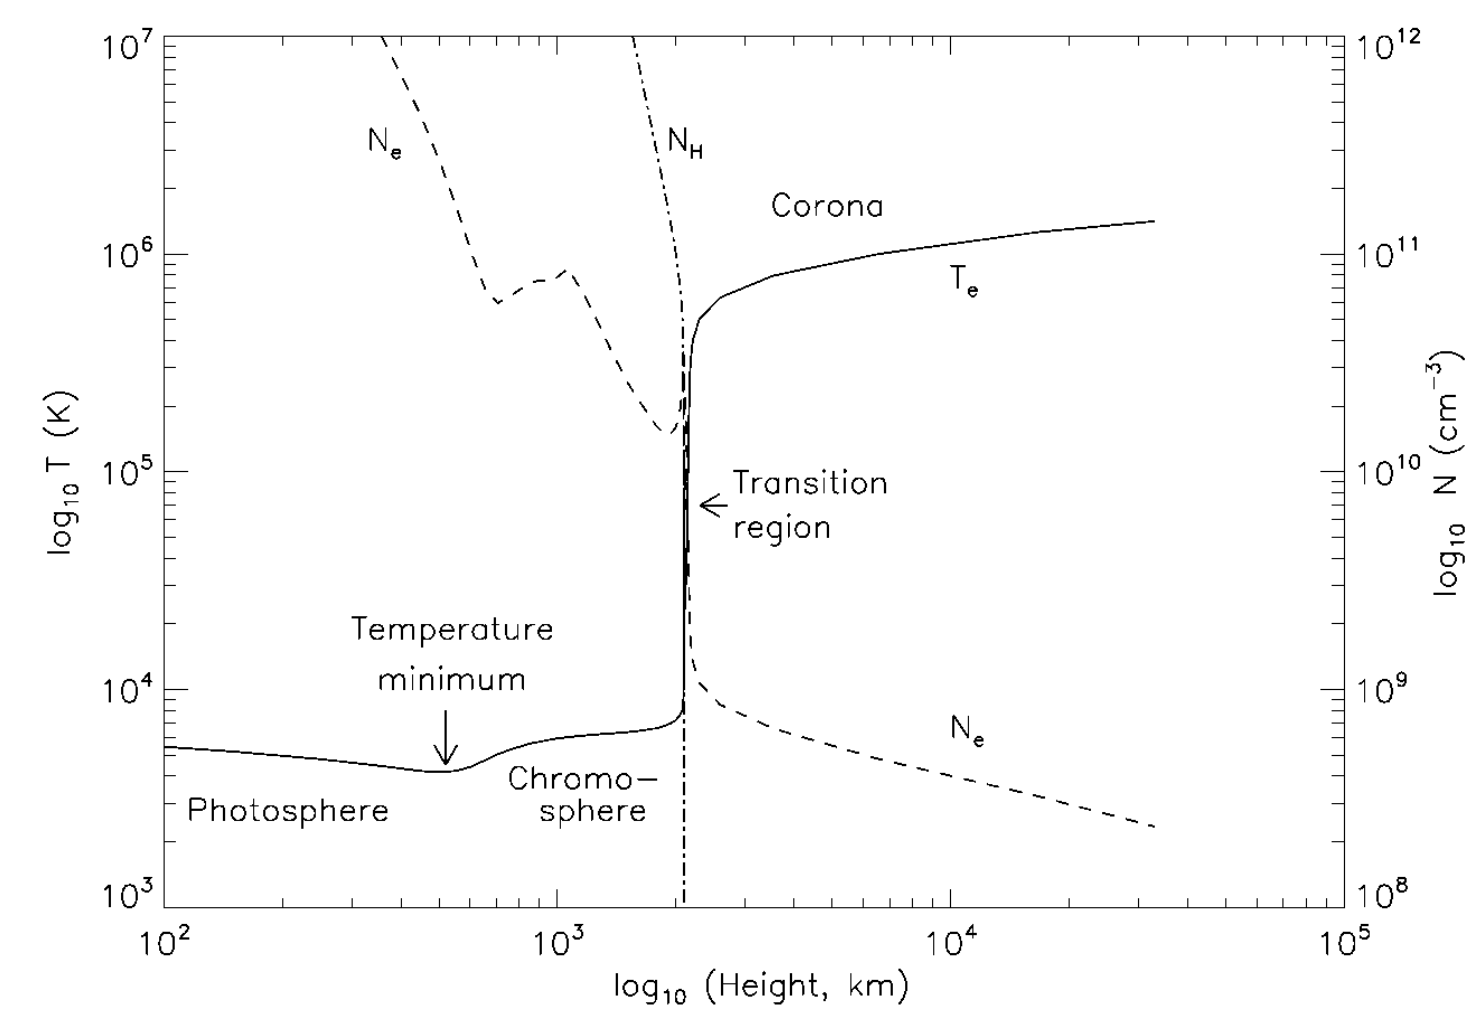
\includegraphics[width = 0.8\linewidth]{Figures/solar_atm.png}
    \caption{The variation of electron temperature (solid line) and electron density ($\mamthrm{N_{e}}$, dashed line) and density of neutral hydrogen atoms ($\mathrm{N_{H}}$, dotted- dashed line) in the solar atmosphere as derived based on the 1-D model calculations by \sr{Ref. here}.}
    \label{fig_solar_atm}
\end{figure}
%% ############# %%

%%%%%%%%%%%%%%%%%%%%%%%%%%%%%%%%%%%%%%%%%%%%%%%%%%%%%%%
\subsection{The Photosphere}\label{photosphere}
%%%%%%%%%%%%%%%%%%%%%%%%%%%%%%%%%%%%%%%%%%%%%%%%%%%%%%%

The Photosphere is defined to be the layer where $\tau_{\lambda~\sim~5000}~=~1$. This is in the green part of the visible spectrum and the Sun is opaque in visible beyond this layer, hence it is called to be the surface of the Sun. This layer is 400-600 km deep and has an effective temperature of 5780 K. The magnetic filed lines arising from the tacholine penetrate the Photosphere and creates a `carpet' over the whole region \citep{priest14}. As mentioned earlier, this is the Solar surface known as the `Quite Sun'(QS). This region exhibits an average magnetic flux density of \textbf{10 -- 50~G}. The QS surface is covered with cells of roughly four size- granule, meso granules, super granules and giant cells. Some regions exhibit much stronger magnetic flux density often associated with highly twisted magnetic field structures. These magnetic features are manifested as sunspots, spicules, bright points etc. 

As the density changes drastically at the Photosphere compared to the convective zone, the thermalized photons from Sun's core start free streaming again, as the mean free path also increases drastically and as a result perturbs the thermal equilibrium (TE from hereon). So, we have to define the thermodynamic quantities of the Photosphere in Local Thermal Equilibrium (LTE from hereon). As we move away from the Photosphere, because the density keeps on decreasing steadily, the LTE conditions also start deviating similarly \citep{philips08}.

%%%%%%%%%%%%%%%%%%%%%%%%%%%%%%%%%%%%%%%%%%%%%%%%%%%%%%%
\subsection{The Chromosphere}\label{chromosphere}
%%%%%%%%%%%%%%%%%%%%%%%%%%%%%%%%%%%%%%%%%%%%%%%%%%%%%%%

The Chromosphere is a highly non-uniform dynamic layer with a thickness of 1500~--~3000~km, with increasing temperature (upto $10^{4}$ K) and decreasing number density. As seen in the fig. \ref{fig_solar_atm}, the temperature of the Chromosphere saturates before the dramatic rise in the transition region. This saturation is attributed to a steady deposition of acoustic energy by creation of shock waves \citep{carlsson07}. The Chromosphere also exhibits a sharp gradient in the plasma $\beta$ factor, non-LTE conditions, dominance of wave motions \sr{Ref. here}. 

%%%%%%%%%%%%%%%%
\begin{figure}[ht!]
    \centering
    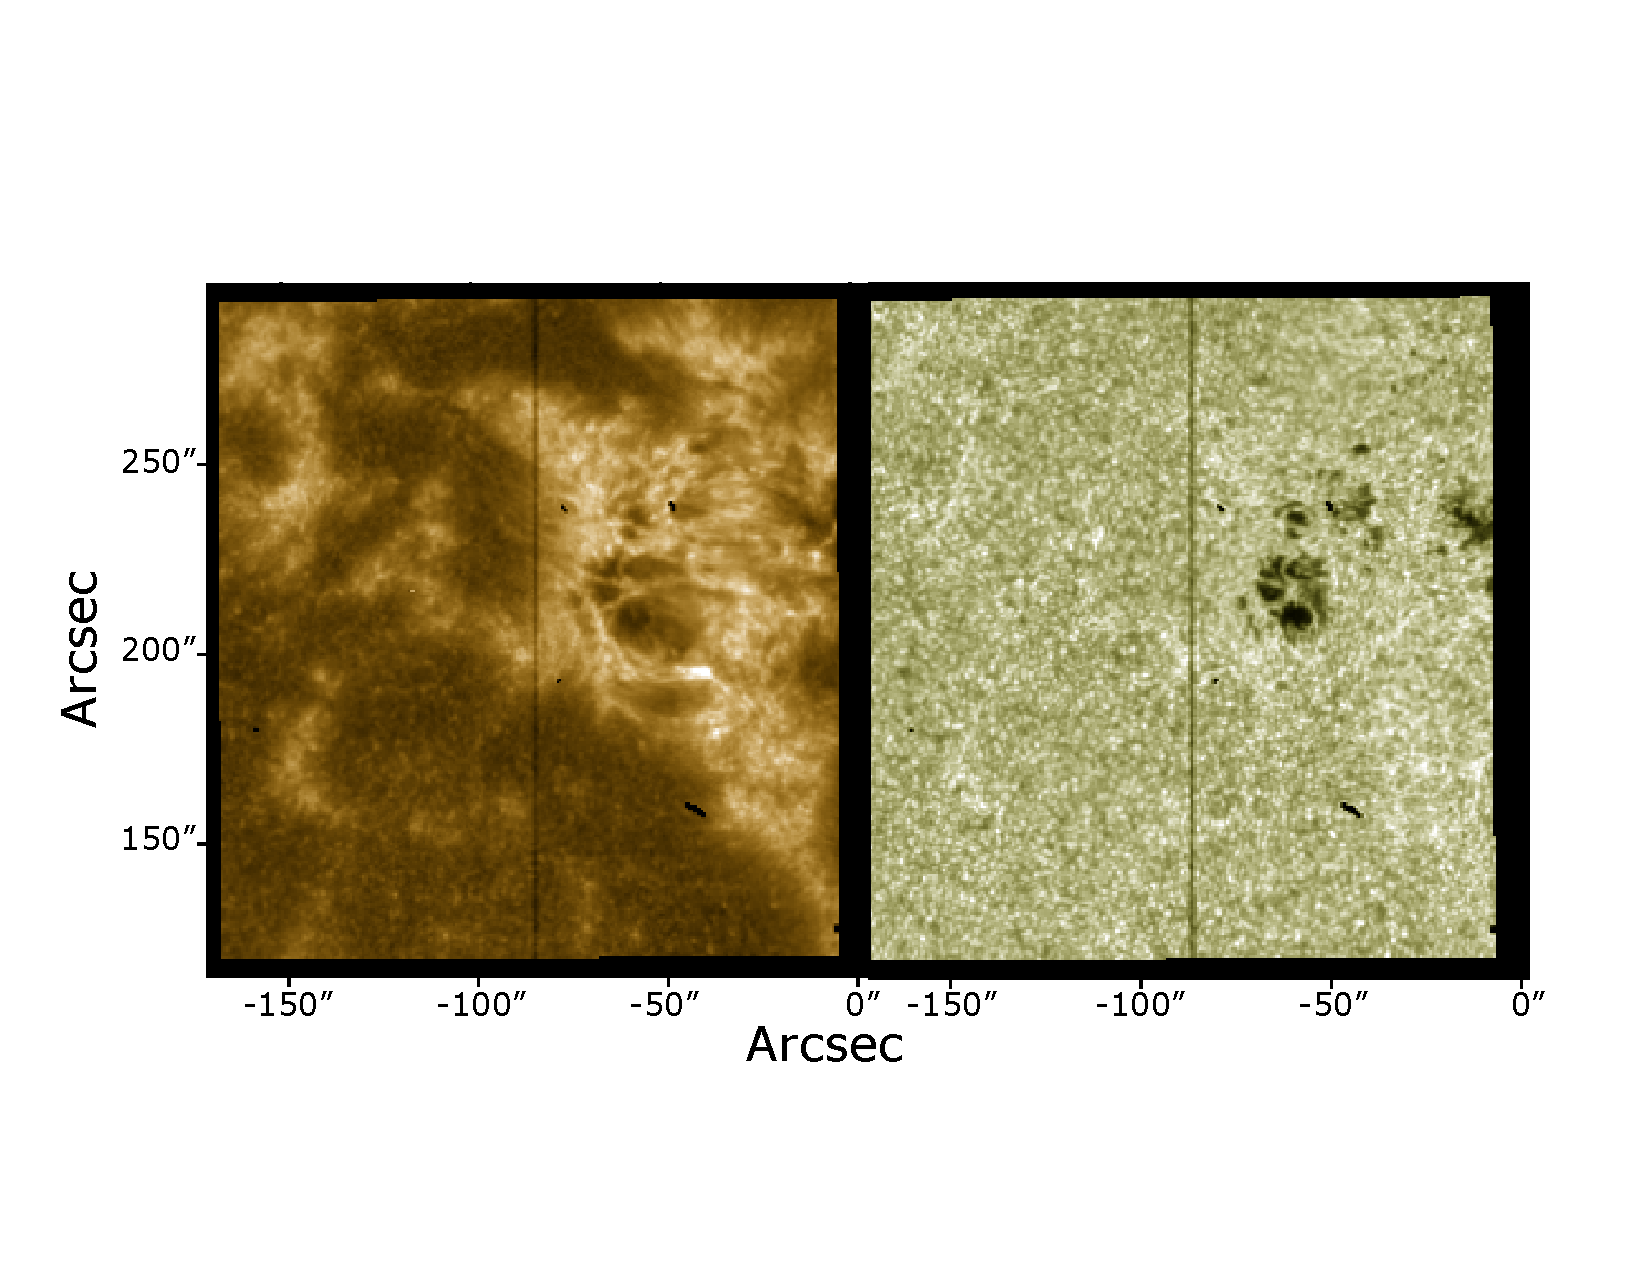
\includegraphics[trim={1cm 3cm 2cm 5cm},clip,width=0.8\textwidth]{Figures/sji_images.pdf}
    \caption{IRIS SJI Slit-jaw images of NOAA AR 13521 on Dec 21st, 2023 in \ion{Mg}{2} 2796 {\AA}~(left panel) showing the upper Chromosphere. The right panel shows the same active region in 2832 {\AA}~continuum corresponding to upper photosphere.}
    \label{fig:sji_features}
\end{figure}
%%%%%%%%%%%%%%%%

In fig.~\ref{fig:sji_features} we show the NOAA AR 13521 in IRIS SJI 2796 {\AA} (left panel) and 2832 {\AA} (right panel). The dark sunspots and plage regions surrounding it are clearly visible in the 2832 {\AA} wavelength window. In the 2796 {\AA} window we see the plage along with light bridges more clearly. 

%%%%%%%%%%%%%%%%%%%%%%%%%%%%%%%%%%%%%%%%%%%%%%%%%%%%%%%%%%%%%%%%%%%
\subsection{The Transition Region}\label{transition-region}
%%%%%%%%%%%%%%%%%%%%%%%%%%%%%%%%%%%%%%%%%%%%%%%%%%%%%%%%%%%%%%%%%%%

The transition region above the Chromosphere is a thin, dynamic layer where we witness a dramatic increase in temperature by two orders of magnitude along with a similar decrease in electron density by nearly 5-6 orders of magnitude which is demonstrated in fig. \ref{fig_solar_atm}. In general the this layer is roughly $\sim$ 100 km in thickness, but that can change depending on various dynamic conditions of Chromosphere($\sim~10^{4}~K$) below, or Corona($\sim~10^{6}~K$) on top. The transition region is generally characterized by the steep change in the temperature, pressure gradients, drastic change in local optical depth and competition between gas pressure and magnetic pressure. The transition region also manifests the ARs as various magnetic features such as small scale brightening, jets, spicules, fibrils etc. 

%%%%%%%%%%%%%%%%%%%%%%%%%%%%%%%%%%%%%%%%%%%%%%%%%%%%%%%%%%%%%%%%%%%
\subsection{The Corona}\label{corona}
%%%%%%%%%%%%%%%%%%%%%%%%%%%%%%%%%%%%%%%%%%%%%%%%%%%%%%%%%%%%%%%%%%%

The outermost layer of the Solar atmosphere is the Corona. The Corona is only visible in naked eyes during the total solar eclipse or via Coronagraphs. It maintains a steady temperature of 1-2 Mk during ambient conditions, but can rise upto tens of MK during solar flares. The coronal continuum spectrum is produced due to Thompson scattering of photons from photosphere off coronal electrons. Corona also emits in various emission lines, e.g. Mg, Fe, Si, S, Ca, O etc. across a wide band of electromagnetic spectrum ranging from X-ray to visible wavelengths. 

Similar to the other layers, the corona exhibits a variety of structures such as ARs, coronal holes, bright points, filaments, flares. The flare arcades are most prominently visible in the Corona. So, most of our existing studies over the last decade has focused on the coronal features of the flares. In fig.~\ref{fig:sji_features} we show one of the most well known and well studied solar eruptions from Aug 31st, 2012. A giant prominence erupted from the south east limb. The erupted prominence material was visible in all AIA channels from 304 \AA~(Chromospheric He II, see fig.~\ref{fig:aia-feature} \textbf{panel (a)}) across all six Coronal channels (\textbf{panel (b){--}(g)}). The sun spots were also clearly visible in HMI magnetogram and continuum (see fig.~\ref{fig:aia-feature} \textbf{panel (h)}). In \textbf{panel (i)} we show the co-aligned AIA 304 \AA, 131 \AA and HMI magnetogram image. The sunspots lie at the base of the erupted prominence, accompanied by the hot thermal plasma associated with the accompanying flare. The novelty of such observation lies in the clear spatial connection across various layers of the sun, connected via energy and momentum transported from one layer to the other. 

%%%%%%%%%%%%%
\begin{figure}
    \centering
    \includegraphics[width=\textwidth]{Figures/aia_features.pdf}
    \caption{Image of the prominence eruption and associated flare from NOAA AR 11562 on Aug 31st, 2012$\sim$19:50 UT. The prominence is visible in all of the AIA channels. We see the coronal holes in AIA 335 \AA~\textbf{(panel c)}. The flare loops of the associated event is visible in AIA 94 \AA~\textbf{(panel e)} and AIA 131 \AA~\textbf{(panel f)}. The sunspots are visible in HMI continuum \textbf{panel (h)}. We show a co aligned map of AIA 304 \AA, HMI magnetogram and AIA 131 \AA~in \textbf{panel (i)}. The spatial association of the sunspots with the hot flareloop plasma and the prominence eruption is clearly demostrated here. }
    \label{fig:aia-feature}
\end{figure}
%%%%%%%%%%%%%




%%%%%%%%%%%%%%%%%%%%%%%%%%%%%%%%%%%%%%%%%%%%
\section{Solar Flares}\label{sol_flr}
%%%%%%%%%%%%%%%%%%%%%%%%%%%%%%%%%%%%%%%%%%%%

Solar flares are the most powerful magnetic events in the solar system. They are described as a sudden increase in brightness in localized areas on Sun. Within tens of minutes, they can release over $10^{32}$ erg of energy, which is emitted across the entire electromagnetic spectrum from radio to gamma rays. They can also launch high energetic particles into the interplanetary medium. Most of the flares occur in magnetic active regions, and the amount of flare energy released is comparable to the free energy stored in the magnetic system. The term "flare" is generally used explicitly for the entire magnetically-driven event's electromagnetic radiation, as it is the most significant fraction of the total energy liberated. The total energy released varies from event to event. It is also known that larger events occur much less frequently than smaller events.

%% ##################################################### %%
\subsection{Brief history of flare observation}\label{sol_flr_1}
%% ##################################################### %%

In September 1, 1859, R.C. Carrington and R. Hodgson observed the first flare in the continuum of white light\citep{carrington1859,hodgson1859}. The localized brightening on the Sun have remained an enigma ever since. We have been observing the local flaring events across all wavelengths from both ground and space based observatories.  Shortly after the observation by Carrington and Hodgson, people started studying the Sun extensively in the H$\alpha$ line which is formed in the Chromosphere, and the reports of flaring events became more and more frequent and progressively more and more complex. No two events were similar, as there were variations observed in source of size, ejections of plasma along with shock waves driving into the interplanetary space. Advances of radio technology during the second world war ensured detection of presence of non-thermal electrons in the solar corona, during military radar operations \citep{hey46}. Around the same time S.E. Forbrush noticed ground level cosmic ray enhancement during major solar flares. These discoveries eluded that the flaring events do not only involve the thermal plasma, but is somehow connects with high energy particles and involves the corona. in the 1950s we started observing the Sun in hard X-rays ($\ge~10~keV$) with rockets and balloons. \cite{peterson59} discovered the first hard X-ray emission during a flare in 1958. Later on, it was deduced from the observations of the enhancements observed in radio and hard X-rays that, the the ejected energetic particles may contain a substantial fraction of the initial energy released \citep{brown71}. The hard X-ray is created by the bremsstrahlung of the electrons colliding into dense material, resulting in a power-law energy distribution. The broadband radio emission from 1 to 100 GHz is created from gyrosynchrotron emission. Finally, observations in EUV and soft X-ray($\le$~10~keV) have shown that the energy released form the flare heats the plasma contained in the coronal loops to temperatures beyond 30 MK. 

%% ################################################################# %%
\subsection{Neupert effect}\label{npt_eff}
%% ################################################################# %%

\cite{neupert68} observed a curious correlation that, the soft X-ray flux during the rise phase of the flare is proportional to the time integral of the centimeter radio flux since the start of the flare. The centimeter radio flux is emitted by relativistic electrons. So, later on the same correlation was found between the hard X-ray flux and soft X-ray flux and can be expressed as,

%%%%%%%%%%%%%%%%%%%%%%%%%%%%%%%%
\begin{equation}\label{npt_eff_eq}
    F_{SXR}(t)~\propto~\int_{t_{0}}^{t}~F_{HXR}(t')~dt'
\end{equation}
%%%%%%%%%%%%%%%%%%%%%%%%%%%%%%%%

This empirical relation is known as the ``Neupert effect''. \cite{neupert68} had already suggested that this may be due to a causal relationship between the thermal plasma and the energetic electrons. The logical explanation is: the soft X-ray mainly originates from a thermal plasma heated by the energy of the flaring event deposited by the flare accelerated electrons. It is important to mention that we know now, Eqn.\ref{npt_eff_eq} is only valid if cooling by conduction of radiation is negligible.

%% ################################################################# %%
\subsection{``Standard'' model of solar flare}\label{sol_flr_std_mod}
%% ################################################################# %%

There were several observations like Neupert effect, which would help us to constrain several phenomenon observed in the flares:

%%%%%%%%%%%%%%%%%%%%%%%%%%%%%%%%%%
\begin{figure}[h!]
    \centering
    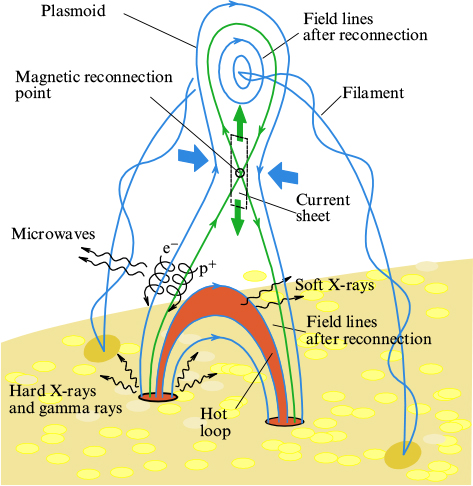
\includegraphics[width=0.5\linewidth]{Figures/phu_63_8_818_f2.jpg}
    \caption{A schematic diagram of the standard model of solar flare (adapted from \cite{lysenko20}).}
\end{figure}
%%%%%%%%%%%%%%%%%%%%%%%%%%%%%%%%%%

%%%%%%%%%%%%%%%%%
\begin{enumerate}
    \item The magnetic reconnetion happens in corona, releasing the magnetic free energy. Electrons and energetic particles from the reconnetion site are accelerated along the realigned magnetic field lines. The accelerated particles that escape along the open field lines towards the earth gives rise to the particle events seen from earth.
    \item The accelerated particles move along the field lines downwards along the magnetic field lines, giving rise to the microwave observations seen from flares via gyro magnetic radiation.
    \item The accelerated particles hit the Chromosphere which is considerably denser than the Corona, giving rise to Hard X-ray and gamma ray observed from the foot points. This also explains why the coronal hard X-ray source is considerably softer than the foot points. The energetic particles deposit their energy into the local Chromosphere, as they go through series of collision and eventually thermalize.
    \item  As the plasma thermalizes, it starts emitting in thermal bremsstrahlung giving rise to the soft X-ray observed. Also, as the energy is deposited into the Chromosphere from the accelerated particles, it heats the local Chromosphere environment it gradually increases the local pressure. 
    \item As the pressure grows, when the pressure gradient builds up enough the local plasma starts expanding upwards(essentially due to buoyancy) and slowly fills up the coronal loops with soft X-ray emitting plasma. This phenomenon is known as "Chromospheric evaporation". This was directly observed later on, in blue-shifted lines of hot material.
    \item This whole scenario explains the Neupert effect. As the energy form the accelerated particles is converted into the soft X-ray emitting plasma, and it builds up over time. That explains the soft X-ray being proportional to the time integral of the hard X-ray flux.
\end{enumerate}
%%%%%%%%%%%%%%%%%

This whole scenario is known as the ``Standard'' model of solar flare. While the standard model is an attempt to explain and unify various kind of differences seen from the numerous flares we observe, there are several cases where the standard model cannot explain the observations. For example, there have been observations of flares where the hard X-ray foot point do not form. It is proposed that in these cases the plasma in the coronal loops is so dense that the accelerated particle collide enough to thermalize within the flare loops before reaching the Chromosphere, defusing the energy more evenly within the loop, rather than dumping it at the base of the loops \citep{veronig02,veronig04}. Another flare which previously occurred at the same region might explain the denser coronal loops \citep{strong84,bone07}.  

%% ################################################################# %%
\subsection{The energectics of solar flares}\label{sol_flr_energ}
%% ################################################################# %%

With an experience of observing solar flares for more than 150 years, remarkably enough, we have barely started scratching the surface of the complexity involved with the solar flares. The re-configuring of magnetic structure, which almost always involves complex geometry, making almost all events unique in some sense. After that the released magnetic free energy is transported across various layers of the sun and converted into various other forms of energy. Considering how the energy is transformed the magnetic energy of the active region that is released after the reconnection into the reconnection outflow jets, the kinetic energy of escaping particles, the thermal and the kinetic energy of the Chromospheric plasma evaporating, the radiative and conductive losses. In case of the eruptive events, there is the added complexity of the kinetic and potential energy of the CMEs, the energy of the shocks and the kinetic energy of the solar energetic particles. 

In order to constrain the models of solar eruptions and various nuanced aspects of it, like magnetic reconnection, particle acceleration, heating etc. detailed quantitative characterization is absolutely necessary. There have been several studies that have tried to quantify the partition between various subsets of the energies. The questions that are particularly important are:

%%%%%%%%%%%%%%%%%%%%%%%%%%%%%%%%%%%%%%%%%%%%%
\begin{itemize}
    \item \textbf{If an active region can have enough free energy to account for the total energy released in the solar flares and/or CMEs.}
    \item \textbf{What is the energy partition between flares and CMEs.}
    \item \textbf{If the non-thermal component have enough energy to power up the thermal component.}
\end{itemize}
%%%%%%%%%%%%%%%%%%%%%%%%%%%%%%%%%%%%%%%%%%%%%

It is generally well known by now that the active region have enough magnetic free energy to power the flare and CME \citep{emslie12,ash17}. The partition of energy between the flare and associated CME is much more fuzzy. \cite{emslie12} found that the flare and CME have energies of same order of magnitude, while \cite{ash17} concluded the flare dominates the CME in-terms of the energy. However the simple question, whether the non-thermal component of the flares have enough energy is still not resolved as even the most recent studies contradict each other in the most puzzling fashion. \cite{warmuth20} discussed the contradictions arising from some of the studies\citep{stosire07,emslie12,inglis14,warmuth16a,warmuth16b,ash17}. The details of the studies can be summarized as follows:

%%%%%%%%%%%%%%%%%%%%%%%%%%%%%%%%%%%%%%%%%%%%%%%
\begin{table}[h!]
    \centering
    \hline 
    \hline
    \resizebox{\textwidth}{!}{%
    \begin{tabular}{||c|c|c|c|c|c|c||}
       Study & No. of flares & GOES class range & Thermal model & Thermal spectrum & Thermal volume & Thermal losses \\
       \cite{stosire07} (S07 from hereon) & 18 & A3-B7 & Isotherm. & RHESSI & TRACE & X \\
       \cite{emslie12} (E12 from hereon) & 38 & C5-X28 & Isotherm. & RHESSI & RHESSI & Rad. \\
       \cite{inglis14} (IC14 from hereon) & 10 & B3-B9 & Multitherm. & RHESSI+AIA & RHESSI & Rad. \\
       \cite{warmuth16a,warmuth16b} (WM16 from here on) & 24 & C3-X17 & Isotherm. & RHESSI+GOES & RHESSI & Rad.,Cond. \\
       \cite{ash17} (A17 from here on) & 188 & M1-X7 & Multitherm. & AIA & AIA & Rad. \\
       \hline
    \end{tabular}}
    \caption{The details of the studies.}
    \label{tab1}
\end{table}
%%%%%%%%%%%%%%%%%%%%%%%%%%%%%%%%%%%%%%%%%%%%%%%

The bolometric energy serves as a representation of the overall energy released during solar flares. Regardless of how energy is released in a solar flare, whether through direct plasma heating, rapid bulk flows, or non thermal particle processes—the ultimate outcome is thermalization and subsequent radiation across the electromagnetic spectrum. Given that bolometric energy encompasses the entire spectrum, it is anticipated to reflect the total energy originally released. It's important to note that this specifically pertains to the energy liberated within the flare and does not encompass the energy associated with a concurrent coronal mass ejection (CME) or filament eruption. \cite{warmuth20} used the bolometric energy released in solar flares, to compare various studies on equal footing. Here we will discuss some of the main issues \cite{warmuth20} identifies comparing these studies.

The calculated thermal energy of all studies show an excellent correlation with the {\it GOES} class. Fig.~\ref{fig:goes-therm} left panel shows the peak thermal energy as a function of peak {\it GOES} flux for all the flares from the five studies. EM12 and WM16 are consistently one order of magnitude lower than the bolometric energy. Interpolation of E12 and WM16 are about half an order of magnitude lower compared to IC14, while S07 is very consistent with the extrapolation. The energies of A17 is about an order of magnitude higher compared to other studies, and even higher than the extrapolated bolometric energy for flares of same class from \cite{kretzschmar11} and E12. There can be several reason of these differences between the studies arising.

A possible reason can be attributed to different thermal models used to model the thermal component of the flares. {\it RHESSI} usually yields a higher temperature and lower emission measure compared to {\it GOES} due to the highly multi thermal nature of the flaring plasma \citep{bataglia05,ryan14,warmuth16a}. Although the {\it GOES} temperature is higher by a factor of 1.4, it is not dependant on the flare class. Along with that, \cite{warmuth20} also investigated whether assuming a isothermal or multi thermal model introduces any differences in the thermal energy estimates. They reported no significant differences due to differences of models (refer to Fig. 2 and the corresponding discussion in \cite{warmuth20}).

%%%%%%%%%%%%%%%%%%%%%%%%%%%%%%%%%%%%%%%%%%%%%%%
\begin{figure}[ht!]
    \centering
    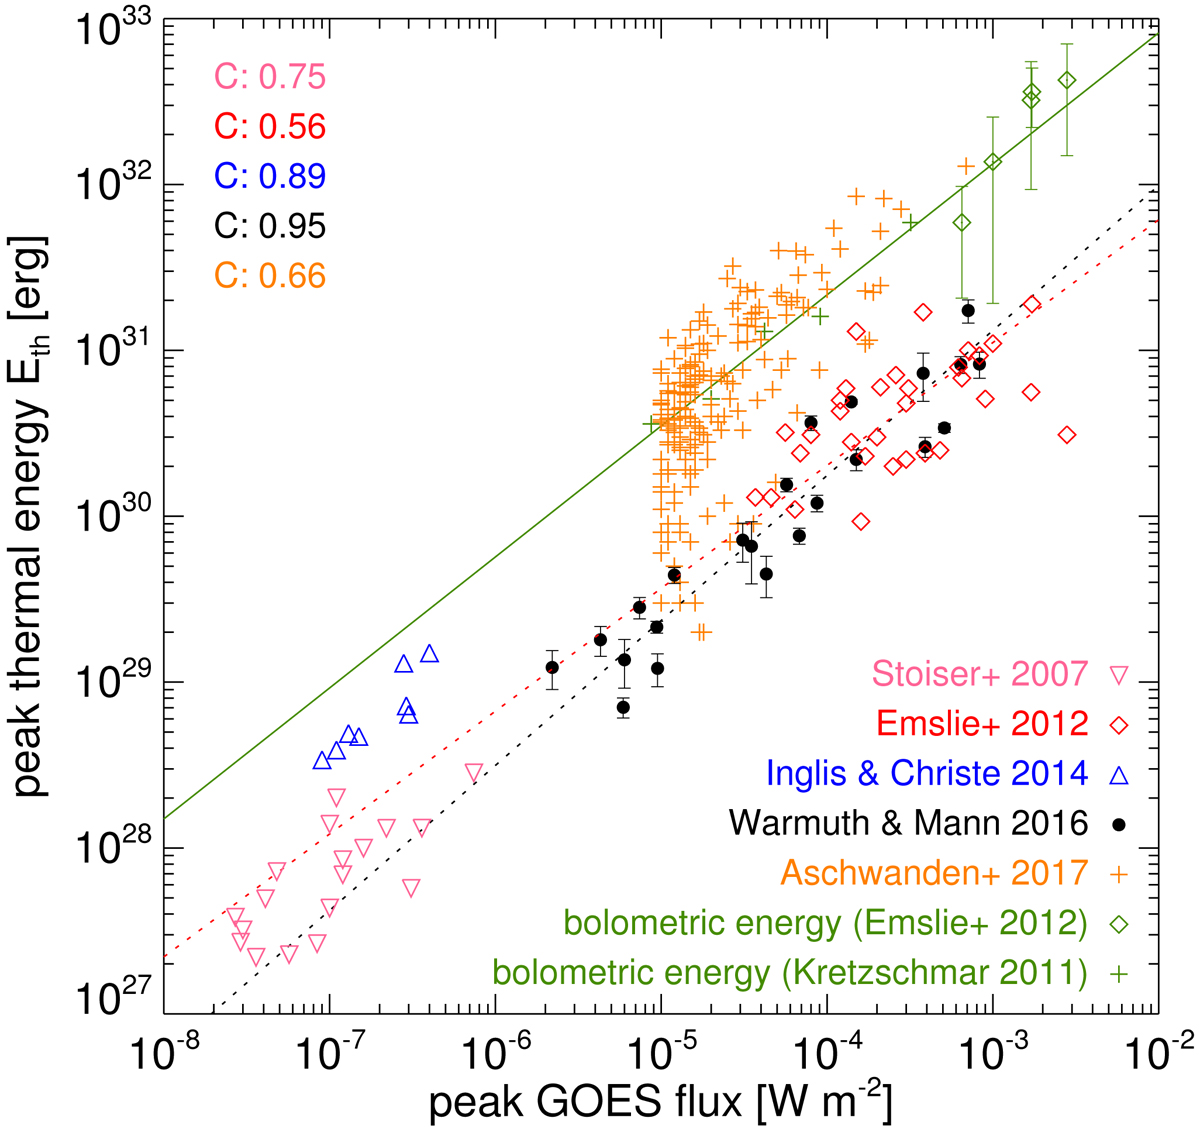
\includegraphics[width=0.45\textwidth,trim={0cm 0cm 0cm 0.02cm},clip]{goes_flux_therm.jpg}
    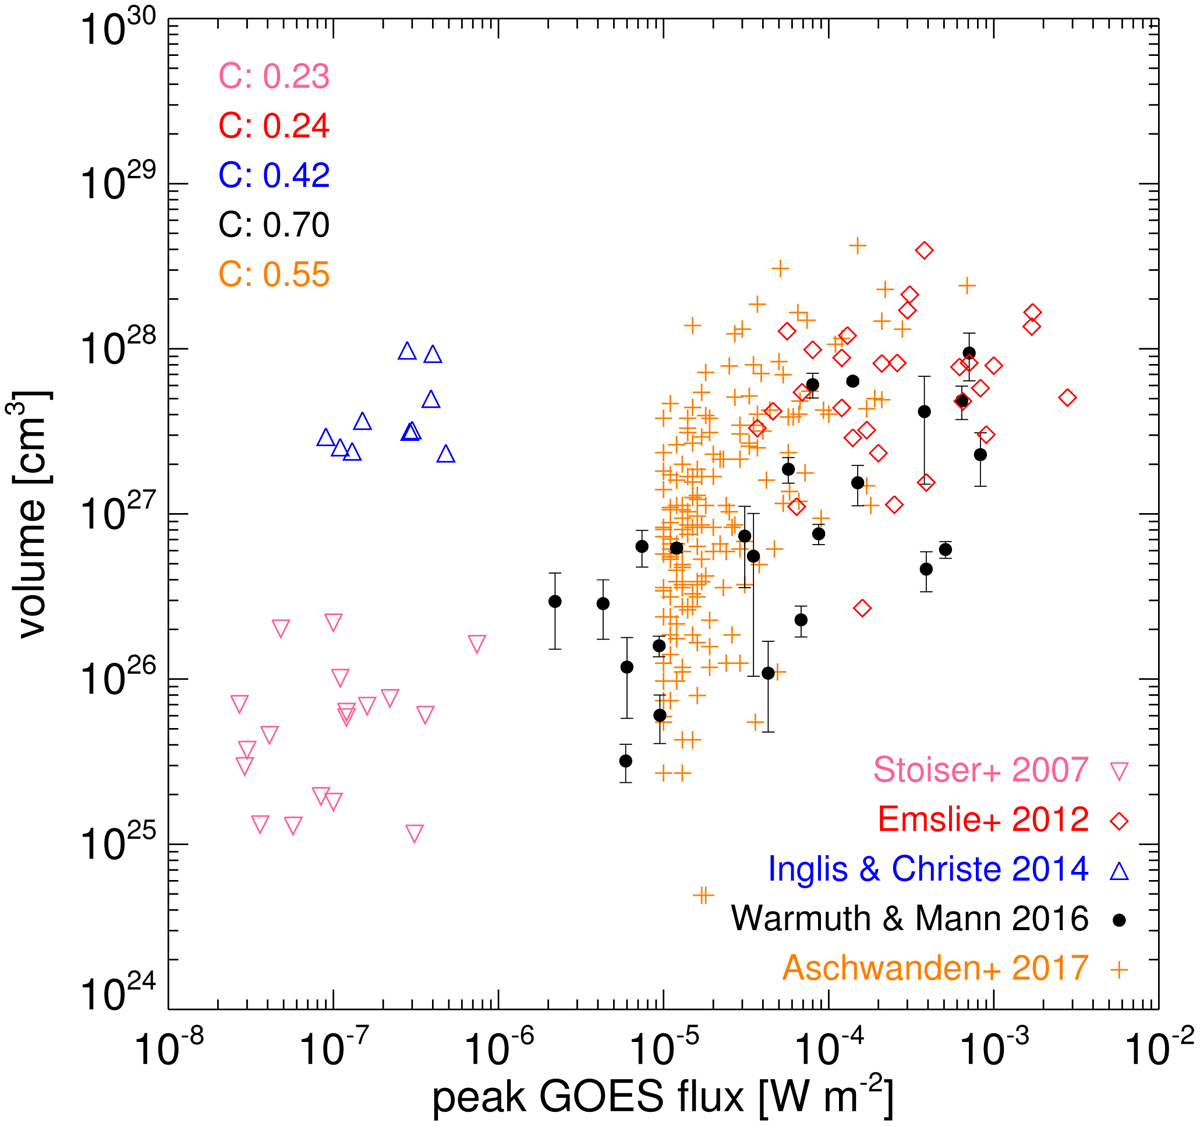
\includegraphics[width=0.45\textwidth,trim={0cm 0cm 0cm 0.02cm},clip]{goes_flux_vol.jpg}
    \caption{{\it GOES} peak thermal energy (left panel) and volume of the thermal plasma (right panel) as a function of the peak {\it GOES} flux for all the flares from five studies (figure credit: \cite{warmuth20}). The C values show the linear correlation coefficient for various studies.}
    \label{fig:goes-therm}
\end{figure}
%%%%%%%%%%%%%%%%%%%%%%%%%%%%%%%%%%%%%%%%%%%%%%%

The thermal energy estimated usually depends on the source volume, $U_{Th}\sim V$. Apart from S07 and A17, all other studies used {\it RHESSI} imaging to estimate the flare volume with a filling factor $f=1$. S07 determined the volume by employing a semicircular loop model, utilizing the cross-sectional area and loop length derived from the observed areas and separations of foot point brightening of 1600  {\AA} by {\it TRACE}. In contrast, A17 estimated the volume based on the flare area exceeding a certain threshold in the emission measure obtained from the spatial synthesis DEM method. Fig.~\ref{fig:goes-therm} right panel shows the volumes used for various studies to estimate the thermal energy as a function of the peak {\it GOES} flux. It is worth noting that the volume estimates from E12 and WM16 align closely, as do those from A+17, despite employing entirely different methodologies. In contrast, the micro flare volumes reported by IC14 are notably larger, ranging from one to two orders of magnitude beyond what would be anticipated based on the findings of the other four studies. Intriguingly, this discrepancy aligns with the additional volume required to account for the higher thermal energies observed in IC14. The uncertainty in detecting volume can be due to the CLEAN algorithm systematically overestimates the source size \citep{warmuth13a}. There has also been studies demonstrating that {\it RHESSI} has difficulties in resolving small sources \citep{dennis09,warmuth13b}, that would be applicable for small thermal sources in the micro flares. This illustrates the requirement for better volume estimation for better estimates of the thermal energy of flares.

We can conclude a few more puzzling questions from these studies as a whole:

%%%%%%%%%
\begin{itemize}
    \item The primary challenge in estimating the thermal energy of the hot plasma stems from determining the temperature distribution of the plasma using Differential Emission Measure (DEM), and the radiating plasma volume.
    \item The dissipation of energy from the hot plasma is substantial. Although there is widespread agreement regarding radiative losses across studies, the extent of conductive losses disagree significantly between the studies.
    \item The non-thermal energy in injected electrons is strongly dependent on the poorly constrained low-energy cutoff.
    \item The thermal and non-thermal energy partition changes with flare class. In smaller flares, there appears to be a deficiency of energetic electrons, whereas in larger flares, the injected non-thermal energy seems to sufficient in powering the thermal component. Does this signify the existence of an additional third heating source?
\end{itemize}
%%%%%%%%%


%% ################################################################# %%
\section{Motivation}\label{sec:mot}
%% ################################################################# %%

The main motivation of this thesis is to add understanding of effects of flares on the surrounding environment in lower and upper solar atmosphere, to answer some of the questions posed above. We have used imaging and spectroscopic observations from multiple space based observatories ({\it e.g.} AIA, HMI, IRIS, XRT, etc.). This research contributes to creating a perspective of flare energetics and its effect on the surrounding plasma environment from Chromosphere to Corona.

The solar flares are the strongest magnetic event in our solar system connecting various layers of the solar atmosphere ({\it e.g.} from Photosphere to Corona), coupled via mass and energy transport. While the Coronal manifestation of solar flares have been studied extensively with several instruments, there are only a few imaging and spectroscopic instruments observing the Photosphere to transition region. These include the {\it IRIS} \citep{iris}, AIA 1600, 1700, and 304  {\AA} \citep{aia} and some the filters of {\it Hinode}/SOT \citep{sot}. In addition to these, we also have had balloon experiment {\it SUNRISE} \citep{sunrise1,sunrise2}, which provided high resolution imaging of the transition regiopn, from the SuFI instrument \citep{sufi}.

This illustrates the necessity of more observatories operating at the transition region wavelengths for more comprehensive understanding about how the solar flares manifest and affect the dynamics and heating of the lower solar atmosphere. In this regard, {\suit} onboard Aditya-L1 will play a crucial role in probing the lower solar atmosphere. The various imaging channels of {\suit} would observe the manifestation of flares in transition region at various heights (NB3 $\implies$ \ion{Mg}{2} k 279.6 nm, NB4 $\implies$ \ion{Mg}{2} h 280.3 nm, NB8 $\implies$ \ion{Ca}{2} h 396.8 nm), further lower in the transition region (NB2 $\implies$ blue wing of Mg window, NB5 $\implies$ red wing of Mg window) and Sunspots and possible signature of umbral brightening due to flares at the Photosphere (NB6 300 nm and NB7 388 nm) in full disk. This would also allow us to probe the interaction of the flaring region, with other active regions on disk, giving us a comprehensive overview of the effect of solar flares and their manifestation in the lower solar atmosphere.

%% ################################################################# %%
\section{Outline of Thesis}\label{sec:outline}
%% ################################################################# %%

The work within this thesis spans across various layers of the solar atmosphere to understand how solar flare couples these layers. It is carried out partly, as various preparatory analysis for {\suit}, forward modelling {\suit} observations, designing the stellar calibration scheme for {\suit}, analysis of existing transition region observations in anticipation of {\suit} observations, analysis of coronal observations of solar flares, and analysis of first solar flare observations by {\suit}. Here we will briefly discuss the structure of the rest of the thesis:

%%%%%%%%%%%%%%%%%%%%%%%%%%%
\begin{itemize}
    \item In chapter \ref{c:chap2}, we review various space based missions available and used in this thesis. We also discuss various analysis techniques used in this thesis. We also motivate the importance of {\suit} and its main science goals. We also briefly discuss the specific questions regarding solar flares we can address with {\suit}.
    \item In chapter \ref{c:chap3}, we discussed some of the initial preparatory analysis we did for {\suit}, including the throughput model for {\suit}, how the filters mounted on {\suit} were chosen, the analysis of spacecraft jitter simulation and what effect it would have on the imaging. We also describe the stellar calibration scheme and the selection criteria for the standard star target. We use a sun as a star spectra to evaluate the calibration scheme with the aforementioned throughput model.
    \item In chapter \ref{c:chap4}, we discuss the forward modelling pipeline developed for {\suit}. We use MPS-Atlas simulation and {\it IRIS} observations, with measured transmission profiles of various optical components and the PSF to forward model {\suit} observations. We also discuss a preliminary version of the deconvolution algorithm that will be deployed in the data reduction pipeline.
    \item In chapter \ref{c:chap5}, we use existing {\it IRIS} observations of three solar flares to probe how the lower solar atmosphere is affected by the flares. The ratio of the \ion{Mg}{2} k and h lines, is a proxy for the optical depth of the surrounding plasma. Hence, we use the observations of \ion{Mg}{2} lines along HMI magnetic field measurements to investigate the effects of magnetic field, if any. \cite{kerr15} conducted a similar study and found signatures of localised heating in the line intensity ratio. We found, that the line intensity ratio shows a correlated increase and decrease with the flare light curve. We argue this to be signature of plasma flow associated with flare, and a change in density of the local environment. This acts as a prelude of what is achievable with {\suit}. We can use a similar method to give full disk context of optical depth, with respect to eruptive events.
    \item We address the issues raised in \S\ref{sol_flr_std_mod} regarding the uncertainties of volume estimation for flaring plasma and its effects on the thermal energy estimation in chapter \ref{c:chap6}. We use observations from {\it SDO}/AIA, {\it STEREO-A}/EUVI, {\it SO}/STIX, {\it GOES}/SUVI to estimate the thermal energy of two solar flares. We propose a new  using existing tools, to use observations from different vantages ({\it e.g.} AIA and EUVI from different angles) to accurately calculate the volume of the flare arcade and estimate the thermal energy. We show that the accurate estimate as a function of time can have effects on the accurate estimation of thermal energy and the partition between the thermal and non-thermal component.
\end{itemize}
%%%%%%%%%%%%%%%%%%%%%%%%%%%
\clearpage
%
\chapter{Existing Solar Observations and Techniques: A bridge towards Solar Ultraviolet Imaging Telescope}\label{c:chap2}
\chaptermark{Solar Observatories and Analysis Techniques}
%UNLIKE IN A REGULAR TEX FILE, DON'T PUT ANY PREAMBLE MATERIAL HERE

%UNLIKE IN A REGULAR TEX FILE, DON'T PUT ANY PREAMBLE MATERIAL HERE

%%%%%%%%%%%%%%%%%%%%%%%%%%%%%%%%%%%%%%%%%%%%
%\section*{Introduction}
%%%%%%%%%%%%%%%%%%%%%%%%%%%%%%%%%%%%%%%%%%%%

\justifying

The remarkable technological progress attained in the last few decades has yielded significant benefits in the form of highly advanced imaging, spectroscopic, and polarimetric instruments designed for astronomical observations. These instruments have empowered us with the ability to scrutinize the Sun with exceptional detail. Specifically, the space based observatories have added new avenues of observing sun. Large portions of the electromagnetic spectra is heavily by Earth's atmosphere \sr{Reference here}.  

The studies within this thesis are using solar observations are multi wavelength analysis of solar flares with both imaging and spectroscopy. In this chapter we describe the details of the instruments and techniques used for our analysis.

%%%%%%%%%%%%%%%%%%%%%%%%%%%%%%%%%%%%%%%%%%%%
\section{Solar Dynamics Observatory}
%%%%%%%%%%%%%%%%%%%%%%%%%%%%%%%%%%%%%%%%%%%%

The Solar Dynamics Observatory \citep[SDO;][]{sdo} is a NASA mission designed to understand the causes of solar variability at various spatio temporal and wavelength scales, as well as its impacts on Earth and the near-Earth environment. It is part of NASA’s Living With a Star program and houses multiple instruments onboard to address its numerous scientific goals. Among the numerous instruments on-board {\it SDO}, we have extensively used data from two instruments – the Atmospheric Imaging Assembly (AIA) and the Helioseismic and Magnetic Imager (HMI).

%%%%%%%%%%%%%%%%%%%%%%%%%%%%%%%%%%%%%%%%%%%%
\subsubsection{Atmospheric Imaging Assembly (AIA)}
%%%%%%%%%%%%%%%%%%%%%%%%%%%%%%%%%%%%%%%%%%%%

AIA \citep{aia} obtains full-disk images of the solar transition region and corona at unprecedented spatio-temporal resolution. The field of view (FOV) covers up to 0.5 $\mathrm{R_{\odot}}$ above the limb. It incorporates several filters at 94 {\AA}, 131 {\AA}, 171 {\AA}, 193 {\AA}, 211 {\AA} and 335 {\AA}, mainly probing the Corona, along with filters at 304 {\AA}, 1600 {\AA}, 1700 {\AA}, and 4500 {\AA}, mainly observing the Chromosphere and Photosphere, providing a total temperature coverage range of 0.06 MK to 20 MK and across various heights. Figure 2.1 illustrates the temperature responses of these filters \citep{borner12}, derived based on the CHIANTI model for solar emissivity \citep{chianti,chianti1}. Under different conditions, these AIA filters observe different plasma phenomena \citep{o'dwyer10}. Typical exposure times range between 0.5 and 3 seconds. Each AIA telescope is accompanied by its own guide telescope to ensure highly accurate image stabilization. For ous analysis, we have extensively used the coronal EUV channel observations from AIA, e.g. 94 {\AA}, 131 {\AA}, 171 {\AA}, 193 {\AA}, 211 {\AA} and 335 {\AA}. These coronal channels observations are usually available with a 12 s cadence.

%%%%%%%%%%%%%%%%%%%%%%%%%%%%%%%%%%%%%%%%%%%%
\subsubsection{Helioseismic and Magnetic Imager (HMI)}
%%%%%%%%%%%%%%%%%%%%%%%%%%%%%%%%%%%%%%%%%%%%

HMI \citep{hmi} obtains images of the Sun across the \ion{Fe}{1} 6173 {\AA} line at six wavelength locations and infers all four components of the Stokes' parameter. Using these observations, various parameters are inferred e.g., Line of Sight (LOS) magnetic field, Doppler velocities, vector magnetic fields etc. We have mainly used the LOS magnetogram for our analysis. These magnetograms have a 0.5{\arcsec} per pixel resolution and 45 s cadence.

%%%%%%%%%%%%%%%%%%%%%%%%%%%%%%%%%%%%%%%%%%%%
\section{Interface Region Imaging Spectrograph (IRIS)}
%%%%%%%%%%%%%%%%%%%%%%%%%%%%%%%%%%%%%%%%%%%%

The Interface Region Imaging Spectrograph \citep[IRIS;][]{iris} is a NASA small satellite explorer mission designed to observe the dynamics of the lower solar atmosphere. IRIS contains a spectrograph and a slit-jaw imager (SJI), observing the chromosphere, the transition region, and the lower corona. It primarily observes the Sun in two pass bands around 1400 {\AA} and 2800 {\AA}. IRIS provides data at high spatial resolution (0.33 {\arcsec} in FUV and 0.4 {\arcsec} in NUV), high time cadence (up to 1 second), and high spectral resolution (12 or 25 m{\AA} per pixel).

IRIS observes three wavelength bands: two in the Far Ultraviolet (FUV) range, spanning 1331.7–1358.4 {\AA} and 1389.0–1407.0 {\AA}, and one in the Near Ultraviolet (NUV) range, covering 2782.7–2851.1 {\AA}. IRIS measures spectra through two primary modes: raster and sit-and-stare. In raster mode, the slit traverses a field of view, capturing spectra from each pixel along its path. When the displacement between consecutive slit positions is comparable to the slit width, it is called dense raster mode; otherwise, it is called sparse raster mode. Alternatively, the instrument may position the slit on a specific region for observation of the Sun. This mode can allow the Sun to naturally rotate across the region or adjust for solar rotation while maintaining continuous observation. This mode is referred to as sit-and-stare. In our analysis, we have used both spectra and SJI imaging from the \ion{Mg}{2} h \& k window and SJI imaging from the \ion{Si}{4} 1402 {\AA} window.

%%%%%%%%%%%%%%%%%%%%%%%%%%%%%%%%%%%%%%%%%%%%
\section{Spectrometer/Telescope for Imaging X-rays (STIX)}
%%%%%%%%%%%%%%%%%%%%%%%%%%%%%%%%%%%%%%%%%%%%

Solar Orbiter \citep[SO;][]{so} is a joint mission between the European Space Agency (ESA) and NASA, launched in February 2020 with the goal of studying the Sun and its dynamic behaviour. The spacecraft aims to provide unprecedented observations of the Sun's polar regions and the inner heliosphere, offering new insights into solar phenomena such as solar wind, coronal mass ejections, and the Sun's magnetic field. We have used observations from the Spectrometer/Telescope for Imaging X-rays (STIX) instrument for our analysis.

 STIX \citep{stix,stix1} is designed to study the Sun's X-ray emissions, providing crucial insights into the processes driving solar flares and other high-energy phenomena. STIX incorporates a set of collimators and detectors to capture high-resolution images of the Sun in X-rays. These images allow scientists to pinpoint the locations and intensities of X-ray emissions associated with solar flares. The instrument covers a broad range of X-ray energies, from approximately 4 to 150 keV, enabling it to observe various aspects of solar activity. STIX can capture X-ray data with high temporal resolution, allowing scientists to study the rapid evolution of solar flares and other transient events in detail. STIX works together with other instruments onboard Solar Orbiter, providing complementary measurements to enhance our understanding of the Sun's dynamic behaviour across different wavelengths and energy ranges.

%%%%%%%%%%%%%%%%%%%%%%%%%%%%%%%%%%%%%%%%%%%%
\section{Extreme Ultraviolet Imager (EUVI)}
%%%%%%%%%%%%%%%%%%%%%%%%%%%%%%%%%%%%%%%%%%%%

Solar Terrestrial Relations Observatory-Ahead \citep[{\it STEREO-A};][]{stereo}, is one of two spacecraft in NASA's STEREO mission, which was launched in October 2006 with the goal of studying the Sun and its dynamic behaviour. {\it STEREO-A} and its twin spacecraft {\it STEREO-B} (Behind) were designed to provide stereoscopic views of the Sun, enabling three-dimensional observations of solar phenomena such as coronal mass ejections (CMEs) and solar flares. Extreme Ultraviolet Imager \citep[{\it EUVI};][]{euvi} is one of the key instruments onboard the {\it STEREO-A} spacecraft. {\it EUVI} is designed to capture images of the Sun in the extreme ultraviolet (EUV) wavelength range. This range of wavelengths is particularly useful for studying the Sun's outer atmosphere, known as the corona, and observing features such as solar flares, coronal loops, and coronal holes. 

{\it EUVI} can capture high-resolution images of the Sun's corona, with spatial resolutions in order of a few arcseconds. It can observe the Sun in 171 {\AA}, 195 {\AA}, 284 {\AA} and 304 {\AA} simultaneously. {\it EUVI} provides continuous observations of the Sun from the STEREO-A spacecraft's vantage point, located slightly ahead of Earth in its orbit around the Sun. This allows {\it EUVI} to monitor solar activity over extended periods and to track the evolution of solar features such as sunspots, flares, and coronal mass ejections (CMEs). We have used 171 {\AA} and 195 {\AA} observations from EUVI for our analysis.

%%%%%%%%%%%%%%%%%%%%%%%%%%%%%%%%%%%%%%%%%%%%
\section{X-Ray Telescope (XRT)}
%%%%%%%%%%%%%%%%%%%%%%%%%%%%%%%%%%%%%%%%%%%%

{\it Hinode} \citep{hinode}, meaning "Sunrise" in Japanese, is a space mission launched by the Japan Aerospace Exploration Agency (JAXA) in collaboration with NASA and the UK Space Agency in September 2006. Also known as Solar-B before its launch, {\it Hinode} is dedicated to studying the Sun's magnetic field and its dynamic behaviour, focusing on understanding the mechanisms driving solar activity and space weather phenomena. The X-Ray Telescope\citep[XRT;][]{xrt} is one of the key instruments aboard the {\it Hinode} spacecraft.

{XRT captures high-resolution solar corona images in X-ray wavelengths, allowing us to study phenomena such as solar flares, coronal loops, etc. Its imaging capabilities enable us to investigate the solar corona's structure, dynamics, and heating mechanisms. XRT utilizes narrow-band filters to isolate specific X-ray emission lines emitted by highly ionized elements in the solar corona. XRT provides continuous observations of the solar corona from the vantage point of the {\it Hinode} spacecraft, which orbits the Earth in a Sun-synchronous polar orbit. This allows XRT to monitor solar activity over extended periods. In our analysis, we used XRT imaging observation from various filters.

%%%%%%%%%%%%%%%%%%%%%%%%%%%%%%%%%%%%%%%%%%%%
\section{Geostationary Operational Environmental Satellites (GOES)}
%%%%%%%%%%%%%%%%%%%%%%%%%%%%%%%%%%%%%%%%%%%%

Geostationary Operational Environmental Satellites (GOES) are a series of weather satellites operated by the National Oceanic and Atmospheric Administration (NOAA) in the United States. These satellites continuously monitor weather conditions across the Americas, including the United States, Canada, Mexico, and parts of South America. GOES data are used by meteorologists and weather forecasters to monitor and predict weather conditions, track severe weather events, and issue warnings and advisories to the public. The continuous monitoring provided by GOES satellites helps improve the accuracy and timeliness of weather forecasts. In addition to monitoring terrestrial weather, GOES satellites also monitor space weather conditions, including solar flares, coronal mass ejections (CMEs), and geomagnetic storms. This information is crucial for forecasting space weather events and assessing their potential impact on satellite communications, navigation systems, and power grids. Among the numerous instruments on-board {\GOES}, we have used data from two instruments extensively {--} X-Ray Sensor (XRS) and Solar Ultra Violet Imager (SUVI).

%%%%%%%%%%%%%%%%%%%%%%%%%%%%%%%%%%%%%%%%%%%%
\subsubsection{X-Ray Sensor (XRS)}
%%%%%%%%%%%%%%%%%%%%%%%%%%%%%%%%%%%%%%%%%%%%

The X-Ray Sensor \citep[XRS;][]{xrs} is an instrument onboard {\it GOES}. The primary function of the XRS is to continuously monitor and measure full disk integrated solar soft X-ray emissions, particularly those associated with solar flares. XRS is designed to detect and measure solar X-ray emissions in two energy bands: short wavelength (0.5 to 4 {\AA}) and long wavelength (1 to 8 {\AA}).

%%%%%%%%%%%%%%%%%%%%%%%%%%%%%%%%%%%%%%%%%%%%
\subsubsection{Solar Ultraviolet Imager (SUVI)}
%%%%%%%%%%%%%%%%%%%%%%%%%%%%%%%%%%%%%%%%%%%%

Solar Ultraviolet Imager \citep[SUVI;][]{suvi} is an instrument aboard {\it GOES}, designed to observe the Sun in the EUV spectrum, providing crucial data for monitoring solar activity and space weather. SUVI captures images of the Sun in 94 {\AA}, 131 {\AA}, 171 {\AA}, 195 {\AA}, 284 {\AA} and 304 {\AA}. These wavelengths are very similar to AIA and provide complementary observations. The FoV of SUVI is rotated by $\sim~45^{o}$, and hence, provides a larger radial distance coverage along the diagonals. In our analysis, we have used SUVI observations from 94 {\AA}, 131 {\AA}, 171 {\AA}, and 195 {\AA}.

%%%%%%%%%%%%%%%%%%%%%%%%%%%%%%%%%%%%%%%%%%%%
\section{Various Plasma Diagnostic Methods}
%%%%%%%%%%%%%%%%%%%%%%%%%%%%%%%%%%%%%%%%%%%%

We employ various techniques throughout this thesis to infer electron density, ion and electron temperature, velocity, thermal structure of the plasma observed in both Chromosphere and Corona. It is standard practice to use atomic databases like CHIANTI \citep{chianti,chianti1} to derive the plasma properties. Below we describe the working principle of the methods used within the scope of this thesis.

%%%%%%%%%%%%%%%%%%%%%%%%%%%%%%%%%%%%%%%%%%%%
\subsection{Differential Emission Measure and Thermal Properties of the Plasma}\label{sec:c2_dem}
%%%%%%%%%%%%%%%%%%%%%%%%%%%%%%%%%%%%%%%%%%%%

Differential emission measure analysis is a commonly employed method with instruments that observe multiple spectral bands to determine the temperature and emission measure of optically thin coronal plasma exhibiting multiple thermal components along a line of sight. However, the inversion process is often challenging due to its ill-posed nature and the frequent lack of sufficient constraints, making it an under determined problem. One of the very first DEM calculation algorithm was {\it xrt\_dem\_iterative}, which was designed and validated for use with XRT data \citep{golub04,weber04}.

The intensity observed by any optically thin imager can be related to the temperature distribution in solar Corona with 
%%%%%%%%%%%%
\begin{equation}
    \mathrm{g_{i}~=~\int_{T}R_{i}(T)~\zeta(T)~dT+\delta g_{i}}
    \label{eqn:dem}
\end{equation}
%%%%%%%%%%%%

In Eqn.~\ref{eqn:dem}, $\mathrm{g_{i}}$ is the counts observed in some specific filter (usually in units of $\mathrm{DN.s^{-1}.pix^{-1}}$), $\mathrm{\delta g_{i}}$ is the observed error, $\mathrm{R_{i}}$ is the temperature response function of the specific filter and DEM(T) describes the thermal distribution of the local plasma  (usually in units of $\mathrm{cm^{-5}.K^{-1}}$). For multiple filter observations, this problem can be posed as a matrix equation in the form of $\Vec{g}~=~\mathbb{R}~\Vec{\zeta}\implies \Vec{\zeta}~=~\mathbb{R}^{-1}\Vec{g}$. However, because of the ill-posed and under-determined nature of the inverse problem, any attempt to invert this set of equations and recovering the DEM results in a significant increase in the noise.

There are several well-characterised methods for inverting the DEM. In this thesis, we have used the method based on regularized inversion developed by \cite{hannah&kontar12}, to infer the thermal distribution of the coronal plasma.Given the under-defined nature of the inverse problem, the problem reduces to a least-square minimizing problem

%%%%%%%%%%%%
\begin{equation}
    \mathrm{||\Tilde{\mathbb{R}}\zeta(T)-\Tilde{g}||^{2}+\lambda||{\bf L}(\zeta(T)-\zeta_{0}(T))||^{2}~=~min}
    \label{eqn:dem}
\end{equation}
%%%%%%%%%%%%

where $\Tilde{\mathbb{R}}~=(\delta g)^{-1}\mathbb{R}$ and $\Tilde{g}~=(\delta g)^{-1} g$. The minimization is performed using the Lagrange multiplier method. {\bf L} is the constrain matrix, $\lambda$ is the regularization parameter and $\zeta_{0}(T)$ is the initial guess solution for the DEM. For further details please refer to \cite{hannah&kontar12}.

With the inverted DEM we get information regarding the distribution of the plasma at a range of temperatures. We can calculate the Emission Measure (EM) given by, $EM=\int_{T}DEM(T)~dT$ (in units of $\mathrm{cm^{-5}}$). The EM is connected to the local plasma density by $EM=\int n_{e}^{2}~dl$. We can also infer the average temperature of the local plasma with the DEM by, $\bar{T}=\frac{1}{EM}\int_{T}DEM(T)~T~dT$.

%%%%%%%%%%%%%%%%%%%%%%%%%%%%%%%%%%%%%%%%%%%%
\subsection{Plasma Velocity from Spectra}
%%%%%%%%%%%%%%%%%%%%%%%%%%%%%%%%%%%%%%%%%%%%

The bulk motion of the plasma along our line of sight can be easily inferred by measuring the red/blue shift of various lines compared to their rest wavelengths. This shift in wavelength is related to the LOS velocity by, $\frac{V_{LOS}}{c}~=~\frac{\Delta \lambda}{\lambda}$.

In addition to the plasma's bulk velocity, several parameters can be inferred from the spectra. The spectral lines are formed due to the transition of electrons between two atomic/ionic energy levels. Instead of a sharp Dirac-delta function, we get the spectra broadened over a wavelength range due to several factors, {\it e.g.}, thermal broadening, Doppler broadening, pressure, optical depth, etc. The FWHM of the spectral line is given by, $\mathrm{FWHM~\sim~\frac{\lambda_{0}}{c}\sqrt{\frac{2k_{B}T}{m}+v_{nth}^{2}+r^{2}}}$. Here, $\lambda_{0}$ is the central wavelength, T is the temperature of the plasma, m is the mass of the ion, $\mathrm{v_{nth}}$ is the non-thermal velocity and r is the given instrumental width. 

The non-thermal broadening of spectral lines is caused by various factors {\, e.g.}, turbulence, wave motion, nano flares, small-scale local flows, magnetic reconnection, etc. All of these broadening appear on top of the Doppler broadening. Accurate estimation of the non-thermal broadening depends significantly on the accurate estimation of the instrumental broadening.

%%%%%%%%%%%%%%%%%%%%%%%%%%%%%%%%%%%%%%%%%%%%
\section{The Solar Ultraviolet Imaging Telescope}\label{sec:suit}
%%%%%%%%%%%%%%%%%%%%%%%%%%%%%%%%%%%%%%%%%%%%

Numerous modern and historical imaging, spectroscopic, and polarimetric instruments have significantly contributed to our comprehension of the Sun and its atmosphere. Several of these instruments, previously discussed, have been utilized in this thesis. While certain instruments are ground-based telescopes, others operate from space. Space-based instruments primarily observe the Sun in Ultraviolet (UV), extreme ultraviolet (EUV), and X-ray bands, capturing radiation emitted from upper atmospheric layers like the transition region and corona, which possess elevated temperatures. Over recent decades, various studies of the Sun have effectively unveiled the physical characteristics of the gas in its upper atmospheric layers using observations recorded by X-ray imaging (e.g., {\it Hinode} X-ray Telescope \citep[{\it Hindoe}/XRT,][]{xrt}) and spectroscopy (e.g., the Spectrometer/Telescope for Imaging X-rays on {\it Solar Orbiter} \citep[{\it SO}/STIX,][]{stix}) as well as extreme ultraviolet (EUV) imaging (e.g., Atmospheric Imaging Assembly on the {\it Solar Dynamic Observatory} \cite[{\it SDO}/AIA,][]{aia}; Extreme ultraviolet Imaging Telescope on {\it Solar and Heliospheric Observatory} \cite[{\it SoHO}/EIT,][]{eit}; Solar Ultraviolet Imager on the {\it Geostationary Operational Environmental Satellites} \citep[{\it GOES}/SUVI,][]{suvi}; the Extreme Ultraviolet Imager on {\it Solar Terrestrial Relations Observatory-A} \cite[{\it STEREO-A}/EUVI,][]{stereo,euvi}; the Extreme-Ultraviolet Imager on {\it SO} \citep[{\it SO}/EUI][]{eui}) and spectroscopy (e.g., \citep[Hinode/EIS,][]{eis}), among others. Instruments such as the {\it Transition Region and Coronal Explorer} \citep[{\it TRACE},][]{trace}, the Solar Ultraviolet Measurements of Emitted Radiation on {\it SoHO} \citep[{\it SoHO}/SUMER,][]{sumer}, and {\it Interface Region Imaging Spectrograph} \citep[{\it IRIS},][]{iris} have facilitated detailed examinations of the chromosphere and the transition region. These missions offer continuous full-disk and Region of Interest (RoI) coverage of the Sun across X-ray and EUV wavelengths. However, the scenario is notably different in the Near-Ultraviolet (NUV) regime, where there is evidently a lack of continuous full solar disk coverage within this wavelength range.

A significant challenge in conducting solar observations in the UV range from the ground is the substantial attenuation caused by the Earth's atmosphere. To overcome this obstacle, one of the pioneering approaches involved the deployment of stratospheric balloon-borne instruments in 1970 and 1971, as documented by \cite{herse79}. This instrument featured a 20 cm telescope capable of imaging the Sun within the 200-460 nm range. Subsequently, the Rasolba balloon experiment utilized a 30 cm telescope equipped with an ultraviolet spectrograph, yielding high-resolution spectra of the Sun spanning 190 to 295 nm \citep{samain85,staath95}. Building upon these endeavors, the Sunrise project \citep{sunrise1,sunrise2} emerged as a balloon-borne observatory designed to observe the Sun in the Near Ultraviolet (NUV) range using a 1 m diameter telescope. Sunrise conducted two flights, in June 2009 and June 2013, respectively, and provided high-resolution imaging at wavelengths of 214, 300, 312, 388, and 397 nm with the Sunrise Filter Imager \citep[SuFI,][]{sufi} in 2009, and at 214, 279, and 397 nm in 2017 \citep{sunrise2}. Additionally, Dopplergrams and vector magnetograms were obtained in \ion{Fe}{1} 525.02 nm using the Imaging Magnetograph eXperiment \citep[IMaX,][]{imax} at various locations on the solar disk. Throughout these flights, Sunrise observed a variety of solar phenomena, including emerging flux events \citep{centeno17}, properties and dynamics of moving magnetic features around pores \citep{kaithakkal17}, proper motion of bright points in quiet sun and active regions \citep{jafarzadeh17}, and properties of fibrils \citep{gaferia17}. These observations underscored the wealth of information carried by this wavelength range and paved the way for full-disk coverage of the Sun in the NUV.

The Solar Ultraviolet Imaging Telescope \citep[SUIT;][]{ghosh16,article}, iss one of the seven payloads aboard the Aditya-L1 mission \citep{adityal1, aditya} led by the Indian Space Research Organization (ISRO). Launched on September 2, 2023, the satellite orbits around the Sun-Earth L1 point in a halo orbit. Equipped with eleven science filters, comprising eight narrow band and three broad band filters, SUIT possesses a distinctive capability to explore various heights within the solar photosphere and chromosphere. This capability aids in understanding the diverse physical processes involved in the transport of mass and energy across different layers of the Sun. Additionally, SUIT offers a unique opportunity to spatially measure the solar spectral irradiance in the Near Ultraviolet (NUV) range, a critical aspect in advancing our comprehension of Sun-climate relationships.

{\suit} is designed to deliver continuous full-disk and Region of Interest (RoI) solar images, boasting a plate scale of 0.7 \arcsec. It possesses the ability to track RoIs while compensating for the effects of differential rotation, as outlined by \cite{suit_algo}. Additionally, SUIT is equipped with onboard intelligence to detect and localize flares, and it can autonomously adjust exposure times to prevent saturation. The primary scientific inquiries targeted by SUIT include \citep{suit_science, suit_main}:

\begin{itemize}
    \item dynamic coupling between the lower and the middle solar atmosphere
    \item measurement of solar spectral radiance in the NUV.
    \item spectral energy distribution of solar flares in NUV
    \item dynamics of chromospheric eruptive phenomena at various spatio temporal scales
    \item Initiation of Coronal Mass Ejections(CMEs) and space weather: the kinematics of erupting prominence during the early phase.
\end{itemize}

%%%%%%%%%%%%%%%%%%%%%%%%%%%%%%%%%%%%%%%%%%%%
\subsection{SUIT \& Solar Flares}\label{sec:suit_and_flare}
%%%%%%%%%%%%%%%%%%%%%%%%%%%%%%%%%%%%%%%%%%%%

Solar flares are the most powerful magnetic events in the solar system. They are described as a sudden increase in brightness in localized areas on Sun. Within tens of minutes, they can release over $10^{32}$ erg of energy, which is emitted across the entire electromagnetic spectrum from radio to gamma rays. They can also launch high energetic particles into the interplanetary medium. Most of the flares occur in magnetic active regions, and the amount of flare energy released is comparable to the free energy stored in the magnetic system. The term "flare" is generally used explicitly for the entire magnetically-driven event's electromagnetic radiation, as it is the most significant fraction of the total energy liberated. The total energy released varies from event to event. It is also known that larger events occur much less frequently than smaller events.

The Solar Ultraviolet Imaging Telescope \citep[SUIT;][]{ghosh16,article} is one of the seven payloads onboard the Aditya-L1 mission \citep{adityal1} of the Indian Space Research Organization (ISRO). With its 11 science filters (3 broadband and eight narrow band), SUIT will have the capability to probe different heights of solar atmosphere in photosphere and chromosphere to help us understand the various processes that transport mass and energy from one layer to another. SUIT will provide full disk as well as partial disk images of the Sun with a pixel size of 0.7". Through SUIT imaging, we would be able to resolve solar flares spatially on the surface of the Sun, for the first time in near ultra-violet (NUV), which will help us to address the questions regarding their build-up and triggering mechanism. In addition, to measure the spatially resolved solar spectral irradiance within the wavelength range that is central for studying the Chemistry of oxygen and ozone in the Stratosphere of Earth's atmosphere.

It has been shown that the majority of flare energy emerges at the visible and UV wavelength range \citep{woods06}. \cite{woods04} showed that about 77\% of the energy is released in the wavelength range > 200 nm, and only ~ 23\% is seen in extreme ultraviolet (EUV) and soft X-ray (SXR), i.e., below 200 nm \citep{Nei_1989,neidig93,kretzschmar11}. Although the energy content in hard X-ray (HXR) is a tiny fraction of the total energy budget, they are still crucial in understanding the energization process \citep{holeman11}. However, to develop a comprehensive understanding of solar flares, it is mandatory to perform multi-wavelength studies of all kinds of flares. This may have implications on the physics of the origin of solar flares and different physics processes and contribute to the solar spectral irradiance as a function of the solar activity cycle. Although we have been observing Sun and Solar flares in various wavelengths, the spectral energy distribution of the radiated energy from the flares is still very poorly understood. The first solar flares were observed from the ground in the visible domain \citep{carrington1859,neidig93}. It is also well known that the flare emission in the visible domain occurs mainly in $H\alpha$ and Ca \Romannum{2} lines \citep{canfield90,falchi92,heinzel94}. However, the lesser understood component of the visible and Near Ultra Violet (NUV) emission is the enhancement of the continuum. The study of the white-light (WL) flares has proven to be very difficult because they have a very short duration and low contrast against the background, making their observation from Earth rare and of poor quality. Also, the flares in NUV are not observable from any ground-based instrumentation as most of the NUV gets absorbed in the upper atmosphere, thus requires space-based observations.

The origin of the WLFs, i.e., the physical process responsible for generating the continuum and its contribution to the overall energy distribution, is still highly uncertain. The question remains whether WLFs are photospheric phenomena due to $H^{-}$ free-free emission or chromospheric phenomena due to H free-bound emission. The more recent studies further constrain the origin of the WLFs to be Chromospheric phenomena, as it has been shown that the WL and HXR foot point centroids are cospatial. Similarly, \cite{krucker15} constrained the cospatial WL and HXR foot points within the chromosphere for three flares. With the help of SUIT, we would be able to localize the WL flares and resolve them on various parts of the Solar disk, which along with observations from Interface Region Imaging Telescope (IRIS), Helioseismic and Magnetic Imager (HMI), would help us localize the source of the WL foot points and also comment on the formation mechanism of the WL itself.

\begin{figure}
    \centering
    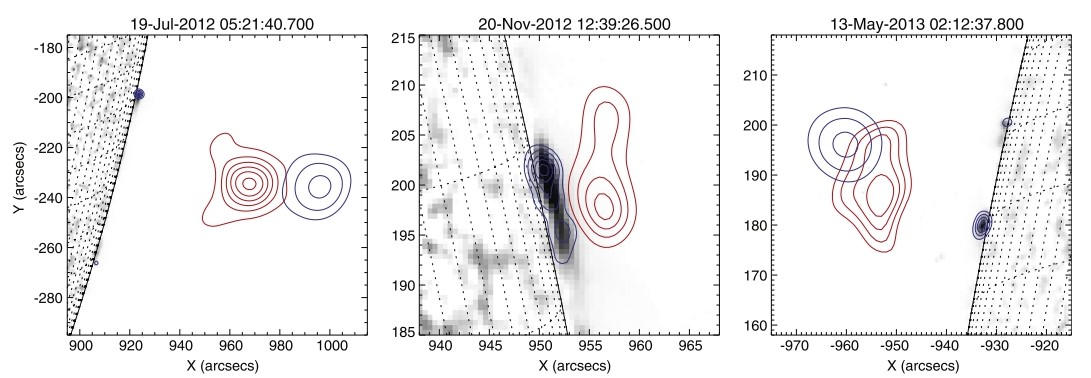
\includegraphics[width = \linewidth]{Figures/Krucker_2015_ApJ_802_19_page-0004.jpg}
    \caption{X-ray and optical imaging of the three flares at the peak time of the impulsive phase: the images are from HMI with the pre-flare image subtracted. The contours represent RHESSI Clean maps in the thermal (red, 12–15 keV) and non-thermal (blue, 30–80 keV) HXR range \citep{krucker15}.}
    \label{fig1}
\end{figure}

The spectral energy distribution of flares is one of the critical areas of interest in the physics of flares. A complete understanding of this will help us decode the physical processes involved in solar flares and help quantify their effects on solar spectral irradiance. Ideally, it would be essential to observe flares at all wavelengths simultaneously with sufficient spatio temporal resolution to figure out the spectral energy distribution of flares. Unfortunately, this is generally not the case, and we have to rely on the sporadic observations made using ground-based instruments in the visible domain. As mentioned earlier, the majority of the flare energy is emitted in the NUV and visible domain. \cite{kretzschmar10,kretzschmar11}, performed statistical studies using a large number of flare observations across a wide energy range. They demonstrated, at the peak of the flare, about 70\% of the total energy was radiated in the continuum visible and NUV channel as illustrated in \ref{tab1}. SUIT would observe and resolve the solar flares within 200-400 nm using 8 NBs and 3 BBs. This, along with IRIS data, would help us comment on the energy distribution of flares of various classes.

%%--------------------------------------------%%
\begin{table}[]
    \centering
    \resizebox{\textwidth}{!}{%
    \begin{tabular}{||m{.1\linewidth}|m{.15\linewidth}|m{.17\linewidth}|m{.17\linewidth}|m{.17\linewidth}|m{.15\linewidth}||}
    \hline
    \hline
        Mean X-ray class & TSI(ergs) & Ratio $\frac{26-34nm}{TSI}$ & Ratio $\frac{0-50nm}{TSI}$ & Ratio $\frac{0.1-0.8nm}{TSI}$ & Ratio $\frac{continuum}{TSI}$\\
        \hline
        X3.2 & 5.9$\times~10^{31}$ & 0.9-0.8\% & 12-9\% & 1.2-1\% & 67\% \\
        M9.1 & 1.6$\times~10^{31}$ & 1.7-0.4\% & 23-5\% & 1-0.4\% & 85\% \\
        M4.2 & 1.3$\times~10^{31}$ & 2.2-0.5\% & 18-6\% & 0.6-0.3\% & 74\% \\
        M2.0 & 5.1$\times~10^{30}$ & 1.7-0.6\% & 18-6\% & 0.7-0.4\% & 69\% \\
        C8.7 & 3.6$\times~10^{30}$ & 1.5-0.5\% & 16-5\% & 0.4-0.2\% & 72\% \\
        \hline
    \end{tabular}}
    \caption{Spectral Energy Distribution from a sample of 2100 flares across various wavelengths\citep{kretzschmar11}.}
    \label{tab1}
\end{table}
%%--------------------------------------------%%

Finally, one of the major question of interest is how the Solar flares affect the Spectral Solar Irradiance (SSI) and Total Solar Irradiance (TSI) variability from a short to much longer, Solar Cycle timescale. \cite{kretzschmar10,kretzschmar11} performed statistical studies using a large number of flare observations across a wide energy range. For this purpose, they used the full Sun observations of Solar flux from Solar and Heliospheric Observatory (SoHO), three visible Solar irradiances from VIRGO/Solar Photometer (SPM) pass bands centred on 402 nm, 500 nm, and 862 nm, respectively, from 1996 to 2008. Additionally, they also use the EUV irradiance in the ranges 0.1-50 nm and 26-34 nm measured by SOHO/Solar EUV Monitor \citep{judge98} and SXR measurements from GOES satellites. They showed that stacked TSI variation profiles during solar flares show variation at more than 2 sigma level during the peak flare time, indicating the presence of flare signals in the TSI measurements.

\begin{figure}[h!]
    \centering
    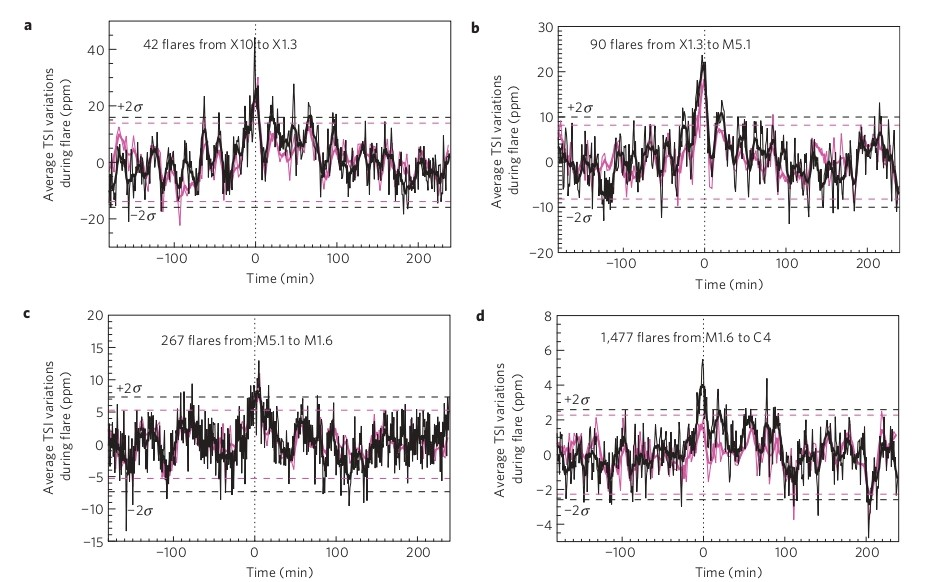
\includegraphics[width = \linewidth]{Figures/nphys1741_page-0002.webp}
    \caption{Averaged TSI variations during flares. The TSI time-series averages over four exclusive sets of solar flares of decreasing amplitude. The black and pink curves correspond respectively to the TSI measured by the PMOV6 and the DIARAD radiometers. The dashed lines correspond to the 95\% confidence levels, while the vertical line denotes the peak time of the flare \citep{kretzschmar10}.}
    \label{fig2}
\end{figure}

This allows us to quantify the solar variability induced be solar flares of various timescales. With the help of SUIT, we would be able to localize the flare locations and study the change in SSI from the local environment in the 11 science filters. This information combined with TSI measurements can allow us to quantify the effect of flares of various energy scales on the TSI variability of the Sun. As, both the TSI and SSI variability directly or indirectly couples with various atmospheric parameters, we can also study the effect the flares have on them. For example, the Earth's atmospheric chemistry and composition respond to any changes in solar UV output in a very nonlinear fashion \citep{haigh07}. Since the number of flares also shows a change with solar activity, it is prudent to ask how much flares contribute to the solar spectral irradiance in NUV. This is particularly important because the irradiance in NUV plays a key role in heating the upper and middle layers of the Earth's atmosphere directly and their coupling with the Stratosphere. It also directly influences the middle and lower atmosphere chemistry and composition via the Ozone-Oxygen cycle.

%NOTE THE LACK OF A BIBLIOGRAPHY CALL IN THIS FILE. BIBLIOGRAPHY WORK HAPPENS OUTSIDE THE CHAPTER TEX FILES.

%NOTE THE LACK OF A BIBLIOGRAPHY CALL IN THIS FILE. BIBLIOGRAPHY WORK HAPPENS OUTSIDE THE CHAPTER TEX FILES.
\clearpage
%
\chapter{Intital preparatory analysis for SUIT}\label{c:chap3}
\chaptermark{SUIT preparatory analysis}
\begin{quote}
{\em ~~~~~~~This thesis chapter originally appeared in the literature as} \\
{authors,
{\em journal reference info}}
\end{quote}

%%%%%%%%%%%%%%%%%%%%%%%%%%%%%%%%%%%%%%%%%%%%
\section{Introduction}\label{secc3_intro}
%%%%%%%%%%%%%%%%%%%%%%%%%%%%%%%%%%%%%%%%%%%%

%%%%%%%%%%%%%%%%%%%%%%%%%%%%%%%%%%%%%%%%%%%%
\section{Throughput model of SUIT}\label{sec:suit_throughput}
%%%%%%%%%%%%%%%%%%%%%%%%%%%%%%%%%%%%%%%%%%%%

%%%%%%%%%%%%%%%%%%%%%%%%%%%%%%%%%%%%%%%%%%%%
\section{Filter Choice for SUIT}\label{sec:filter_choice}
%%%%%%%%%%%%%%%%%%%%%%%%%%%%%%%%%%%%%%%%%%%%

%%%%%%%%%%%%%%%%%%%%%%%%%%%%%%%%%%%%%%%%%%%%
\section{Photometric, Radiometric \& Spectral Calibration of SUIT}\label{sec:suit_cal}
%%%%%%%%%%%%%%%%%%%%%%%%%%%%%%%%%%%%%%%%%%%%
\clearpage
%
\chapter{Forward modelling SUIT observations}\label{c:chap4}
\chaptermark{SUIT forward model}
\begin{quote}
{\em ~~~~~~~This thesis chapter originally appeared in the literature as} \\
{authors,
{\em journal reference info}}
\end{quote}
\justifying

%%%%%%%%%%%%%%%%%%%%%%%%%%%%%%%%%%%%%%%%%%%%%%%%
\section{Introduction} \label{sec:intro}
%%%%%%%%%%%%%%%%%%%%%%%%%%%%%%%%%%%%%%%%%%%%%%%%

The remarkable technological progress attained in the last few decades has yielded significant benefits in the form of highly advanced imaging, spectroscopic, and polarimetric instruments designed for astronomical observations. These instruments have empowered us with the ability to scrutinize the Sun with exceptional detail. While some of these are ground based telescopes, the others operate from space. Primarily, space-based instruments observe the Sun in Ultraviolet (UV), extreme ultraviolet (EUV), and X-ray bands, capturing radiation from upper atmospheric layers such as the transition region and corona
, which emit due to their elevated temperatures. Various studies of the Sun over the last few decades have successfully uncovered the physical properties of the gas in the upper layers of the solar atmosphere using the observations recorded by X-ray imaging ({\it Hinode} X-ray Telescope \citep[{\it Hindoe}/XRT,][]{xrt}) and spectroscopy (the Spectrometer/Telescope for Imaging X-rays on {\it Solar Orbiter} \citep[{\it SO}/STIX,][]{stix}) and extreme ultraviolet (EUV) imaging (Atmospheric Imaging Assembly on the {\it Solar Dynamic Observatory} \cite[{\it SDO}/AIA,][]{aia}, Extreme ultraviolet Imaging Telescope on {\it Solar and Heliospheric Observatory} \cite[{\it SoHO}/EIT,][]{eit}, Solar Ultraviolet Imager on the {\it Geostationary Operational Environmental Satellites} \citep[{\it GOES}/SUVI,][]{suvi}, the Extreme Ultraviolet Imager on {\it Solar Terrestrial Relations Observatory-A} \cite[{\it STEREO-A}/EUVI,][]{stereo,euvi}, \textbf{the Extreme-Ultraviolet Imager on {\it SO} \citep[{\it SO}/EUI][]{eui}}) and spectroscopy \citep[Hinode/EIS,][]{eis}, among many others. The {\it Transition Region and Coronal Explorer} \citep[{\it TRACE},][]{trace}, \textbf{the Solar Ultraviolet Measurements of Emitted Radiation on {\it SoHO} \citep[{\it SoHO}/SUMER,][]{sumer}} and the {\it Interface Region Imaging Spectrograph} \citep[~{\it IRIS},][]{iris} allowed us to probe the chromosphere and the transition region in detail. These missions provide us with continuous full disk and Region of Interest (RoI) coverage of the Sun over the X-ray and EUV wavelengths. The situation is rather different in the Near-Ultraviolet (NUV) regime. There is clearly a lack of continuous coverage of the full solar disk in this wavelength range. 

One of the key challenges of carrying out Solar observations in the UV regime from ground is the strong attenuation by the Earth's atmosphere. To circumnavigate this, one of the first stratospheric balloon-borne instrument was flown in 1970 and 1971 by \cite{herse79}. The instrument carried a 20 cm telescope that imaged the sun in 200{--}460 nm. The Rasolba balloon experiment was composed of a 30 cm telescope with an ultraviolet spectrograph. They obtained high resolution spectra of the Sun in the spectral range 190 {--} 295 nm \citep{samain85,staath95}. Sunrise \citep{sunrise1,sunrise2} is a balloon-borne observatory that followed up these instruments to observe the Sun in the Near UltraViolet (NUV) regime with a telescope of 1 m diameter. It has flown twice, in June 2009 and June 2013, respectively and provided us with high resolution imaging in 214, 300, 312, 388 and 397~nm with the Sunrise Filter Imager \citep[SuFI,][]{sufi} in 2009 and at 214, 279 and 397~nm in 2017 \citep{sunrise2}, Dopplergrams and vector magnetorams in \ion{Fe}{1} 525.02 nm with the Imaging Magnetograph eXperiment \citep[IMaX,][]{imax} at various locations on the Solar disk.  During these two flights, along with quiet sun and active regions, Sunrise observed various solar phenomenon e.g. emerging flux events \citep{centeno17}, properties and dynamics of moving magnetic features around pores \citep{kaithakkal17}, proper motion of bright points in quiet sun and active regions \citep{jafarzadeh17}, properites of fibrils \citep{gaferia17} etc. These observations demonstrated the wealth of information this wavelength range carries and opened the path for full disk coverage of the Sun in the NUV. 


The Solar Ultraviolet Imaging Telescope \citep[SUIT;][]{ghosh16,article} is one of the seven payloads onboard the Aditya-L1 mission \citep{adityal1, aditya} of the Indian Space Research Organization (ISRO), launched on September 2, 2023. The satellite is placed in a halo orbit around the Sun-Earth L1 point. With its eleven science filters (eight narrow band and three broad band), {\suit} has the unique capability to probe different heights in the solar photosphere and chromosphere; helping us to understand various physical processes responsible for the transport of mass and energy from one layer to another. Moreover, SUIT provides the unique opportunity to measure the spatially resolved solar spectral irradiance in the NUV, which is central to our understanding of Sun climate relations. 

{\suit} is designed to provide full-disk and RoI images of the Sun continuously, with a plate scale of 0.7{\arcsec}. It has the capability of tracking the RoIs while compensating for the differential rotation \citep{suit_algo}. Moreover, it is also capable of detecting and localizing flares with on-board intelligence and can also automatically control the exposure time to avoid saturation. The main science questions that {\suit} aims to address are \citep[][]{suit_science,suit_main}: 

\begin{itemize}
    \item Coupling and dynamics of the solar atmosphere: {\it How is energy channeled and transferred from the photosphere to the chromosphere in the solar atmosphere?}
    \item Sun-Climate Relationship: {\it Understanding the Variability of Solar Spectral Irradiance (SSI) and NUV radiance of various features on the Sun.}
    \item Solar Flare Dynamics and Energy Distribution: {\it At Which wavelength Do flares emit the majority of their energy, and what proportion of this energy is from the NUV Range? What is the spectral energy distribution of flares?}
    \item Physics of eruptions at various spatio-temporal scales: {\it what physical processes drive eruptive phenomena observed at various spatio-temporal scales in the Photosphere and Chromosphere?}
\end{itemize}

In this work we aim to forward model the observations recorded by {\suit} using the Max Planck Institute/University of Chicago Radiative Magneto Hydrodynamics \citep[MURaM,][]{muram} and MPS-ATLAS codes as well as observations recorded by the Interface Region Imaging Spectrograph (IRIS). MURaM is a three-dimensional (3D) MHD code designed to facilitate realistic simulations of magneto-convection and other related magnetic features (such as pores, sunspots and emerging flux) in the upper convection zone and photosphere. The simulation includes the effects of non-gray radiative transfer, partial ionization, full compressibility and open boundary conditions. The simulation gives us various physical quantities such as density, temperature, magnetic flux density etc. The MPS-ATLAS \citep{witzke12} code, which solves the radiative transfer equation vary rapidly with the help of opacity distribution functions, can be applied to the model atmosphere obtained from MURaM  to synthesize the spectrum. Since the MURaM simulation cubes used here do not include the non-local thermodynamic equilibrium, these cannot be used to forward model the observations for chromospheric filter. Therefore, for this purpose, we utilize the observations recorded by~{\it IRIS} in \ion{Mg}{2} lines. 

Since the observations taken by an instrument such as {\suit} are convolved with their respective response functions, we need to have a de-convolution algorithm in place that can be employed in the data reduction pipeline. Here, we present the de-convolution algorithm employed in the data reduction pipeline for {\suit}. To ensure the reliability of the deconvolution algorithm, we must treat the radiation coming from the solar model (or from the~{\it IRIS} spacecraft) in exactly the same way as the solar photons are treated by the instrument. I.e. they must be spatially convolved by the point spread function (PSF) of the instrument at the relevant wavelength and spectrally filtered and attenuated. For this purpose we use measured filter profiles and PSFs. %\sks{Is this addition correct? Without it, readers may wonder at much of Sect. 2.}

The rest of the paper is structured as follows. In \S\ref{sec:inst} we briefly describe details of the payload and present the effective area of various filter combinations. We present our method for calculating intensity maps from model atmospheres computed from MURaM, using MPS-ATLAS in \S\ref{sec:mps}. We present the measured point spread function (PSF) for the eleven science filters of {\suit} and the effects of the instrument PSF on the imaging in \S\ref{sec:psf} with the calculated intensity maps presented in \S\ref{sec:mps} and~{\it IRIS} observations. Finally, we summarize and conclude in \S\ref{sec:con}.

%%---------------------------------------------------
\begin{figure}
    \centering
    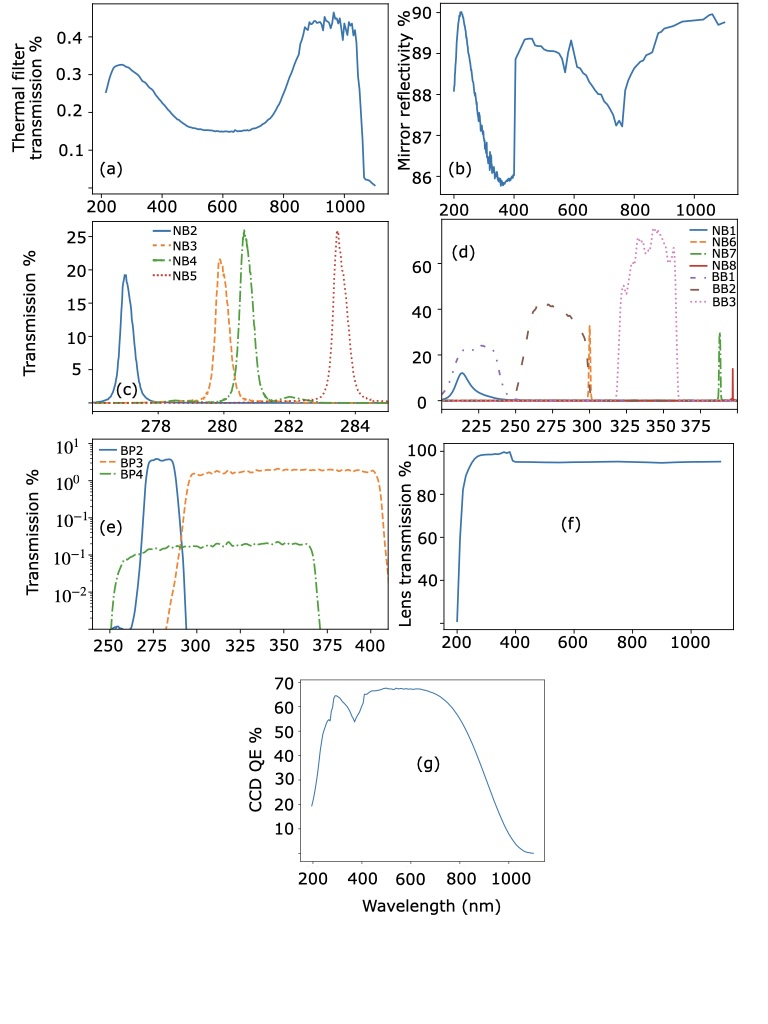
\includegraphics[trim={0.4cm 3.8cm 1cm 0cm},clip,width=0.75\textwidth]{optical_comp.jpeg}
    \caption{Transmission as a function of wavelength of thermal filter (panel a), science filters (panels c and d), band pass filters (panel e) and the field corrector lens (panel f). We also plot the reflectivity of the mirrors in panel b and the quantum efficiency curve of the detector (panel g). Labels on x-axes are wavelength in nanometers.} 
    \label{fig:tras_prof}
\end{figure}
%%---------------------------------------------------

%%---------------------------------------------------
%\begin{figure}
 %   \centering
  %  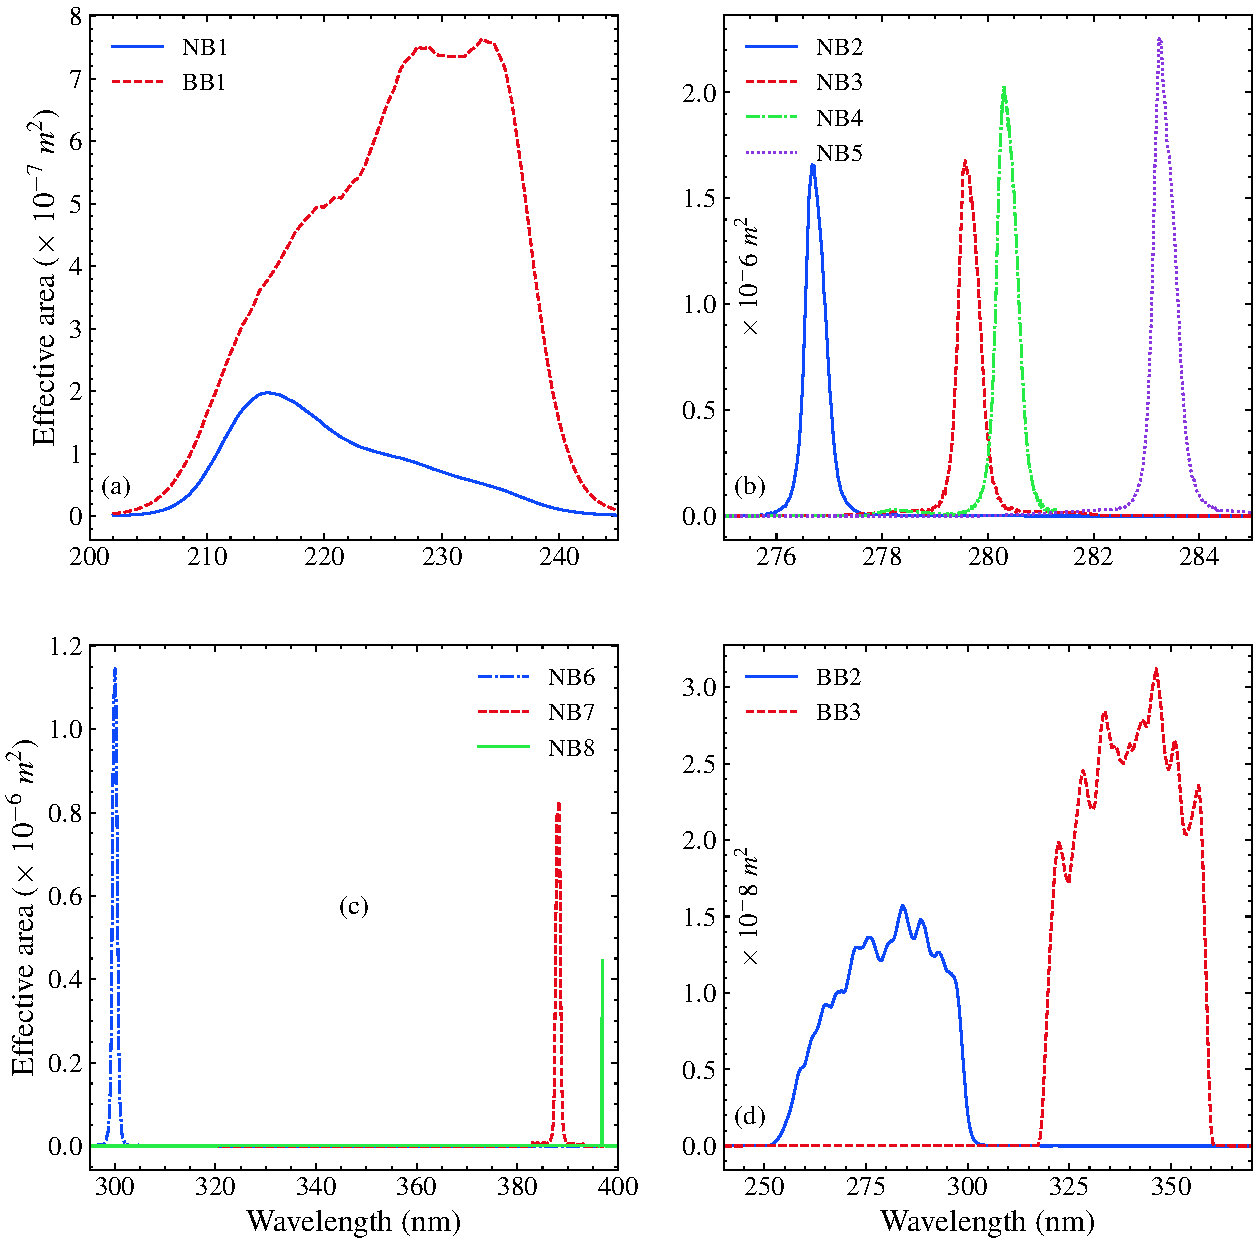
\includegraphics[trim={0cm 0cm 0cm 0cm},clip,width=0.75\textwidth]{eff_area.pdf}
   % \caption{The effective area curves for all science filters as labeled.}
    %\label{fig:eff_area}
%\end{figure}
%%---------------------------------------------------

%%---------------------------------------------------
\section{The Instrument} \label{sec:inst}
%%---------------------------------------------------
The {\suit} is a two mirror off-axis telescope, which is designed to image the Sun with a plate scale of ~0.7{\arcsec}, and a field of view (FOV) of 0.75{\degree} on a 4096~$\times$~4096 charged coupled device (CCD), which has 12~$\mu$m pixel size. %Figure~\ref{fig:layout} shows a schematic diagram of the {\suit}. 
The entrance of the payload consists of an entrance door mechanism and a thermal filter(TF). The TF \cite[][]{thermal_filter_1, thermal_filter_2} is designed to cut down most of the incoming visible ($\approx$ 99.75\%) and infrared($\approx$ 99.5\%) radiation and transmits a very small fraction ($\approx$ 0.3\%) of the radiation within 200{--}400~nm. The transmitted light passes through the telescope, gets reflected from the primary and secondary mirrors, respectively, to arrive at the shutter mechanism, which is located between the secondary mirror and the filter wheels. For more details on the instrument, see \cite{article,suit_main}.

%%---------------------------%%
\begin{figure*}
    \centering
    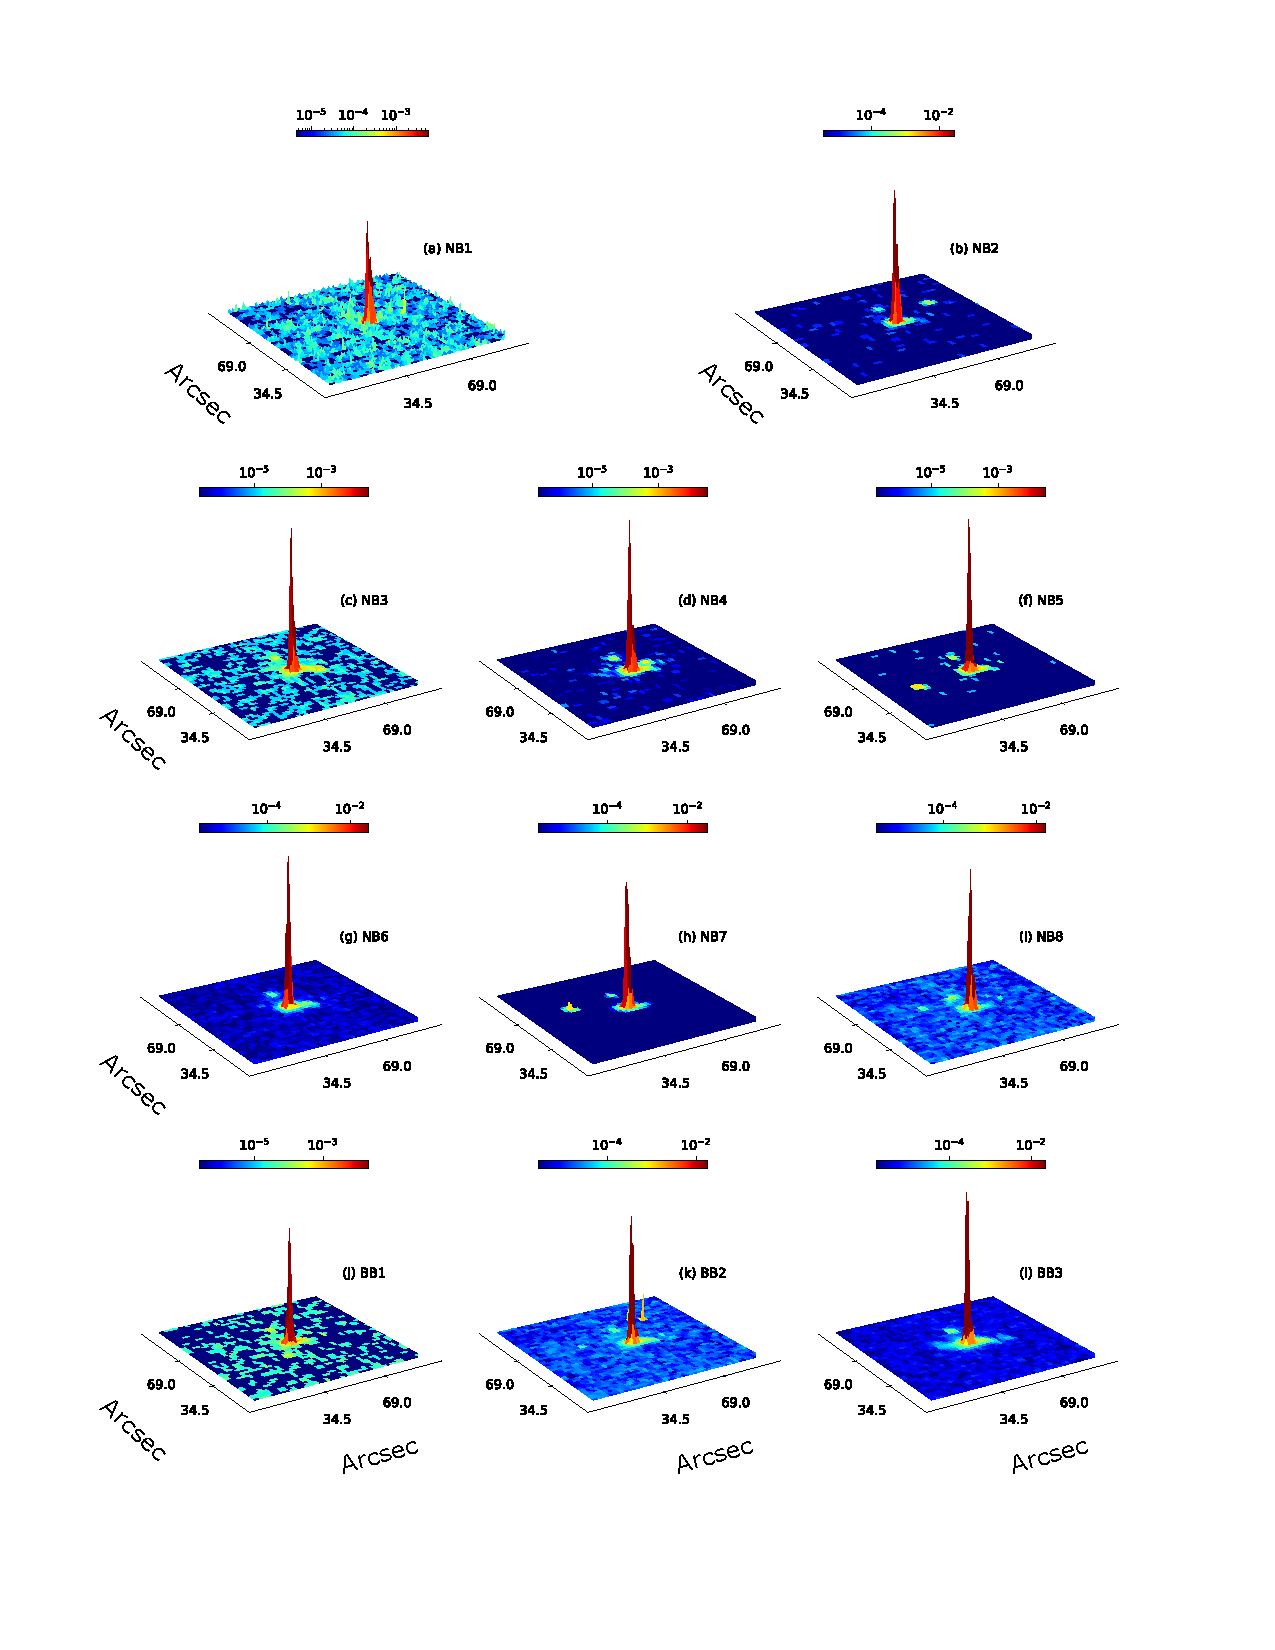
\includegraphics[trim={1.7cm 3cm 2cm 1.5cm},clip,width=0.8\textwidth]{Figures/suit_psf_3d.pdf}
    \caption{The measured PSF for the various filter combinations. The colormap is area normalized, i.e. the sum of the PSF over the total area is unity.}
    \label{fig:psf_3d}
\end{figure*}
%%---------------------------%%

{\suit} has 11 science filters (first column Table~\ref{tab:science_filters}), and five band pass filters (BPFs), which are used to keep the photon flux within the dynamic range of the CCD. Out of these five band pass filters, while two are the spare copies NB8 and BB1, we designed three additional band pass filters namely, BP2, BP3 and BP4. These 16 filters are mounted on two filter wheels (FWs), each holding eight filters. The combination of the appropriate science filter and band pass filter is achieved by rotating the two filter wheels independently. Note that secondary piece of BB1 is used as combination filters NB1 and BB1. Similarly, NB8 is combined with an identical NB8. Between the FWs and the detectors a focusing lens is mounted on a piezo motor, which can be used as a focusing mechanism.  Fig.~\ref{fig:tras_prof} displays the the transmission profile of the individual components in the optical path.

%%---------------------------%%
\begin{figure*}
    \centering
    %\hspace{-1cm}
    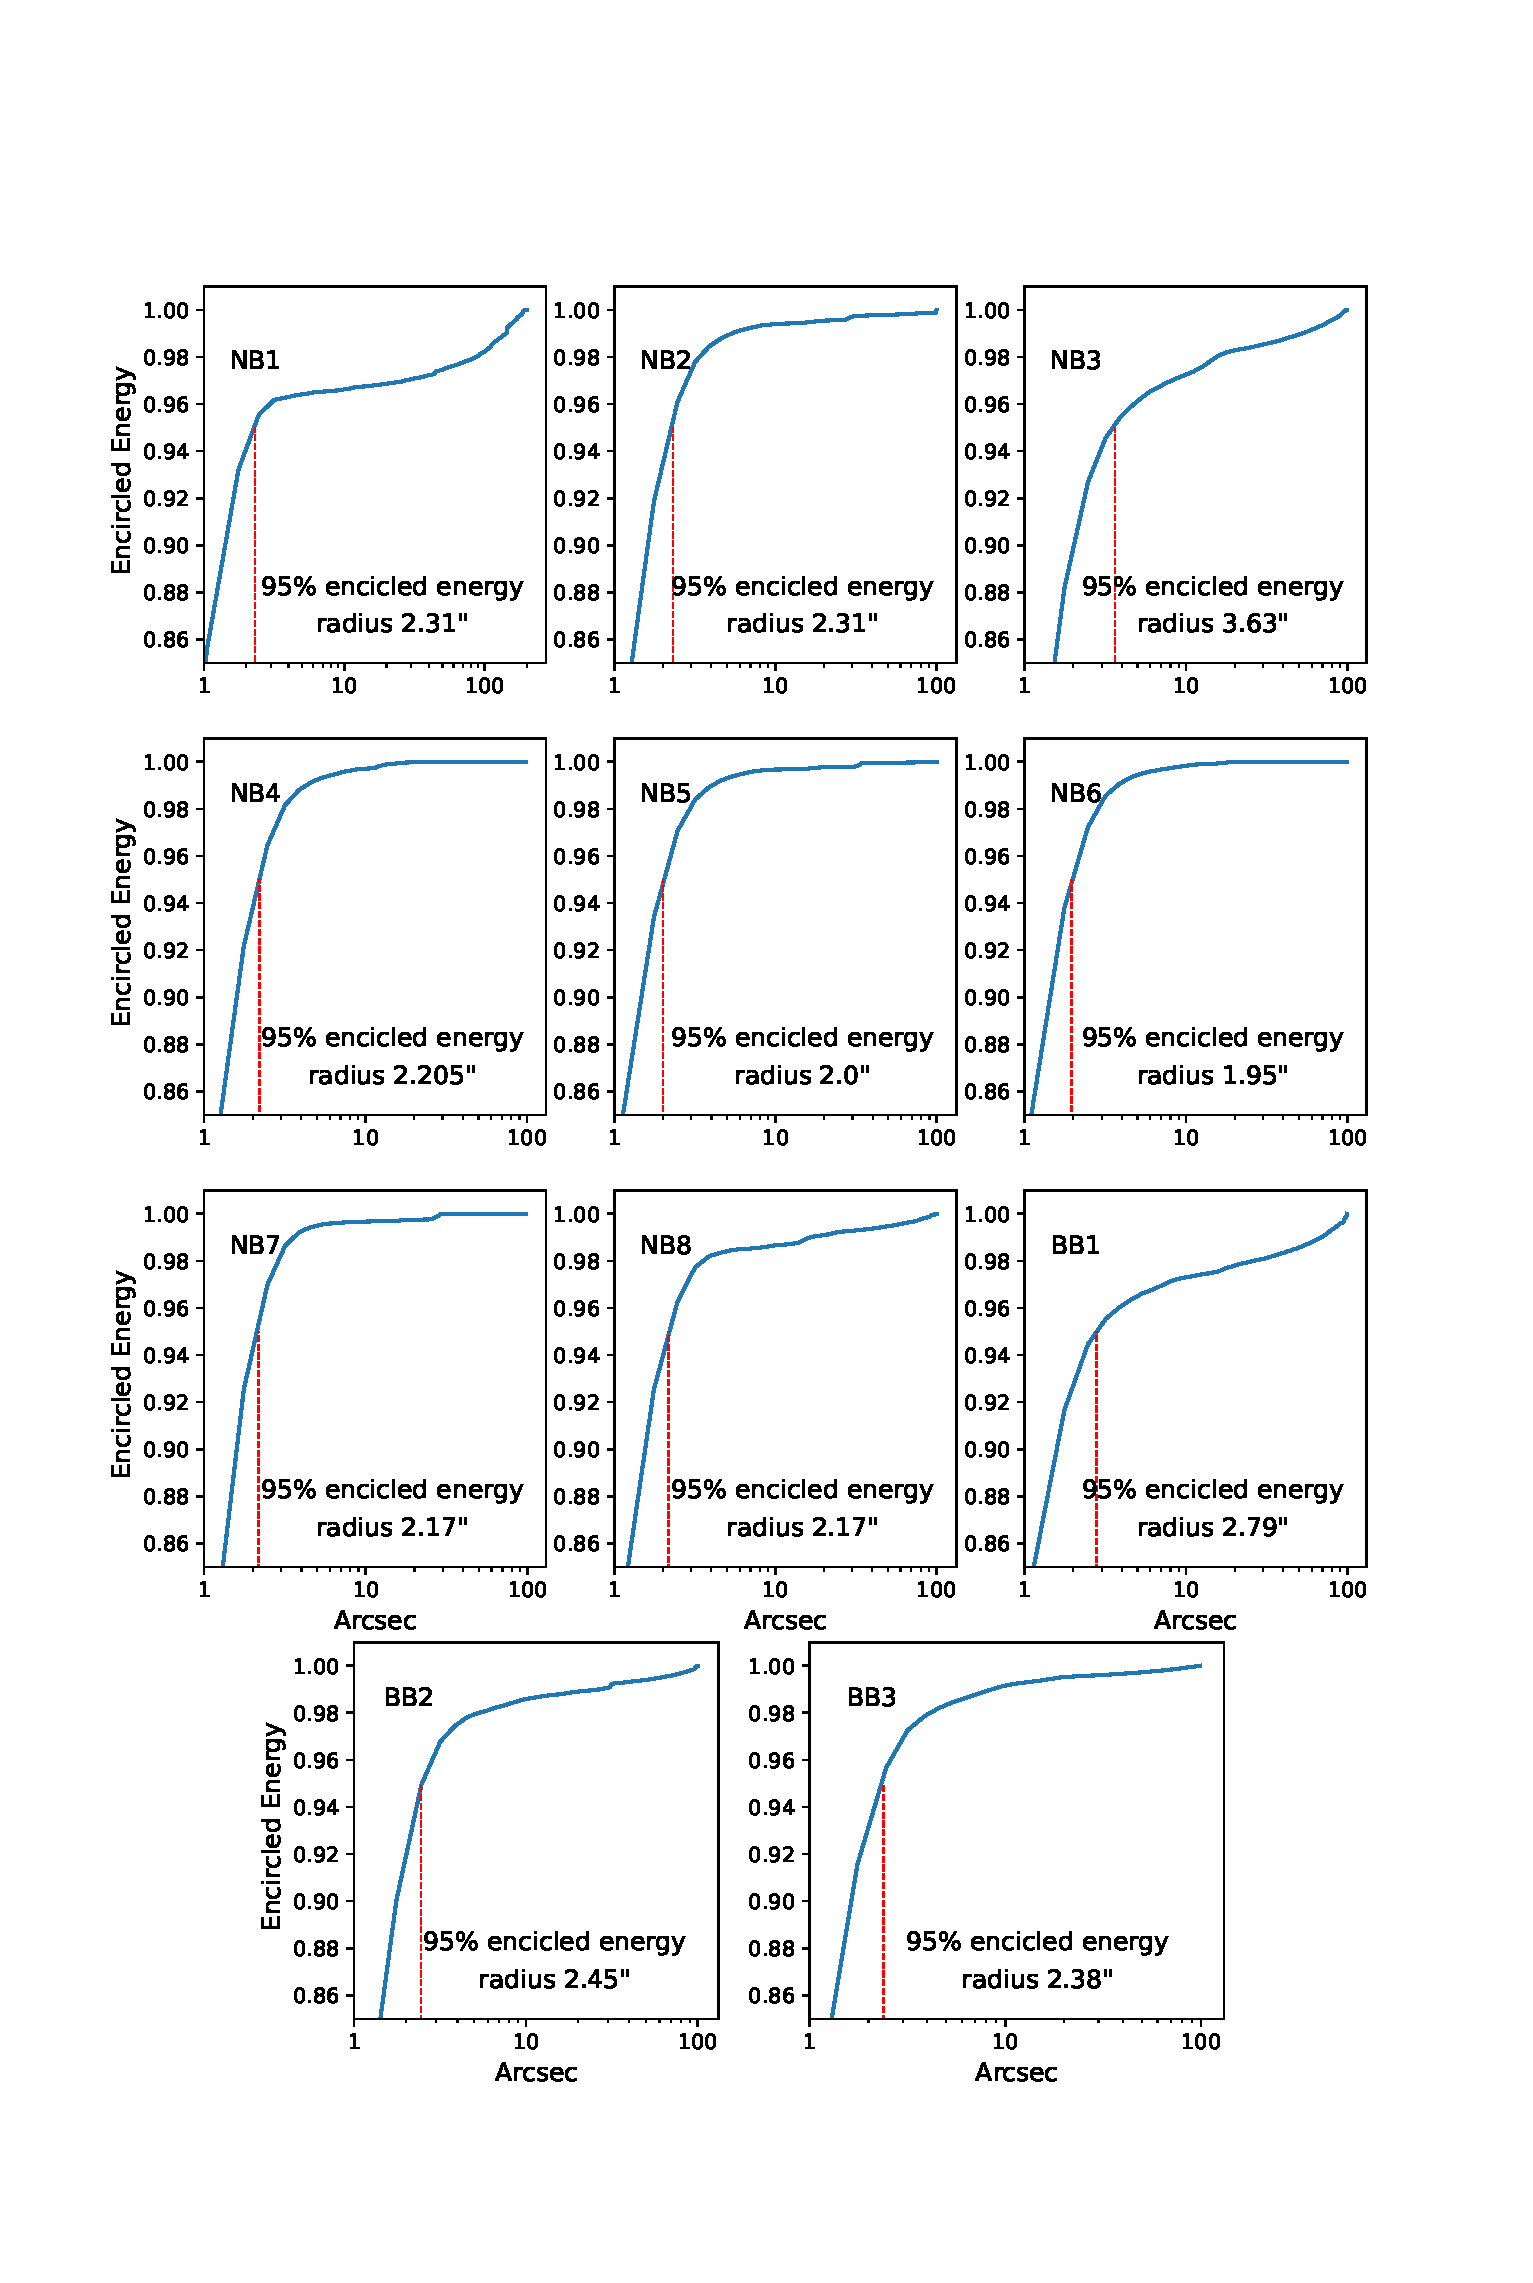
\includegraphics[trim={1.5cm 3cm 2.5cm 4cm},clip,width=0.6\textwidth]{psf_ese_2.eps}
    \caption{The encircled energy curve for the measured PSF. The 95\% encircled energy radius are marked with the vertical dashed red line. The angular scale of the 95\% encircled energy radius is also quoted in each panel for the specific filter combination.}
    \label{fig:psf_ese}
\end{figure*}
%%---------------------------%%

%%---------------------------------------------------------------
\begin{figure*}
    \begin{center}
    \resizebox{0.9\textwidth}{!}{%
        \begin{tikzpicture}[node distance=2cm]
            \node(muram)[io]{Model 3D atmospheres simulated by the radiative-MHD code MURaM};
            \node(slice)[io,right of=muram,xshift=3.5cm]{Slice the MURaM cubes and interpolate them to various $\mu$ values};
            \node(filter)[io,below of=muram,yshift=-1cm]{Use \suit~ science filter profiles accounting for all the optics on the ray path};
            \node(odf)[io,right of=filter,xshift=3.5cm]{Generate ODF tables for various filters using the MPS-ATLAS code};
            \node(rdt)[io,right of=odf,xshift=3.5cm,yshift=1.5cm]{Use ODF tables and 1D ray-atmospheres from the 3D MHD cube to carry out RT calculations using MPS-ATLAS};
            \node(int)[io,below of=rdt,yshift=-3cm]{Integrate the generated spectra for each pixel of the cube over the wavelength range of the filter profile to generate the intensity map};
            \node(conv)[io,left of=int,xshift=-4.5cm]{Convolve the total emergent intensity maps with relevant \suit~ PSF and bin to \suit~ plate scale to create mock observation};
            \draw[arrow](muram)--(slice);
            \draw[arrow](slice)--(rdt);
            \draw[arrow](filter)--(odf);
            \draw[arrow](odf)--(rdt);
            \draw[arrow](rdt)--(int);
            \draw[arrow](int)--(conv);
        \end{tikzpicture}}
        \caption{The flow chart shows the entire process of generating the simulated intensity maps, from the data cubes and characterizing the filters.}
        \label{fig:flow}
    \end{center}
\end{figure*}
%%---------------------------------------------------------------
%%---------------------------------------------------------------
\subsection{The Point Spread Function (PSF) of SUIT} \label{sec:psf}
%%-----------------------------------------------------------------

In Fig.~\ref{fig:psf_3d}, we plot the measured Point Spread Function (PSF) at the centre of the CCD for the different science filter combinations for {\suit}. The PSFs are highly peaked at the centre. The scattered light background becomes clearly visible due to the log scaling of the color bar and is more than two orders of magnitude lower than the peak.

Fig.~\ref{fig:psf_ese} shows the encircled energy curve for the measured PSFs for various filter combinations normalized to the total integral of unity. The vertical dashed lines in each plot show the radius within which 95\% of the incident light falls. For example, for the NB2 filter, 95\% of the incident light from a point source arrives within a 2.31{\arcsec} radius ($\sim$ 4.6{\arcsec} diameter) and 5\% of the light falls outside that region. Note that while the 95\% diameter is 4.6{\arcsec}, the PSF is strongly peaked. The overall diameter is considerably larger than the highly peaked part of the PSF because of the presence of a pedestal in the PSF. The pedestal is visible in all of the cases at the base of the central peak, although it is about 2 order of magnitude lower in all the cases (see Fig.~\ref{fig:psf_3d}). In some cases (e.g. NB1, BB2 etc.) a few or multiple smaller peaks apart form the pedestal are also visible. Similar radii for other filters are quoted in the corresponding panels of Fig.~\ref{fig:psf_ese}. The encircled count curves help us characterize the stray light for various filter combinations.

%%%%%%%%%%%%%%%%%%%%%%%%%%%%%%%%%%%%%%%%%%%%%%%%%%%%%%%%%%%%%%%%
\section{Forward Modeling SUIT intensity maps using MPS-ATLAS and MURaM} \label{sec:mps}
%%%%%%%%%%%%%%%%%%%%%%%%%%%%%%%%%%%%%%%%%%%%%%%%%%%%%%%%%%%%%%%%

One of the essential steps of characterizing the science filters was to conduct a thorough throughput modeling for the concerned filter combinations. However, quantifying the effects of the wavelength response of the optical components and the PSF on the spatially resolved observations, as well as the contrast variation, requires detailed modeling with resolved simulations of the Sun's surface. For this purpose, we use the MPS-ATLAS code. It is an updated version of the well established ATLAS9 \citep{atlas9} code that can efficiently generate Opacity Distribution Functions (ODFs), model atmospheres, and calculate emergent spectra in local thermodynamic equilibrium (LTE) for a given wavelength range by solving radiative transfer (RT) equation in plane parallel geometry using the assumptions of local-thermodynamic-equilibrium (LTE).

%%%%%%%%%%%%%%%%%%%%%%
\begin{wrapfigure}{l}{0.45\textwidth}
    \centering
    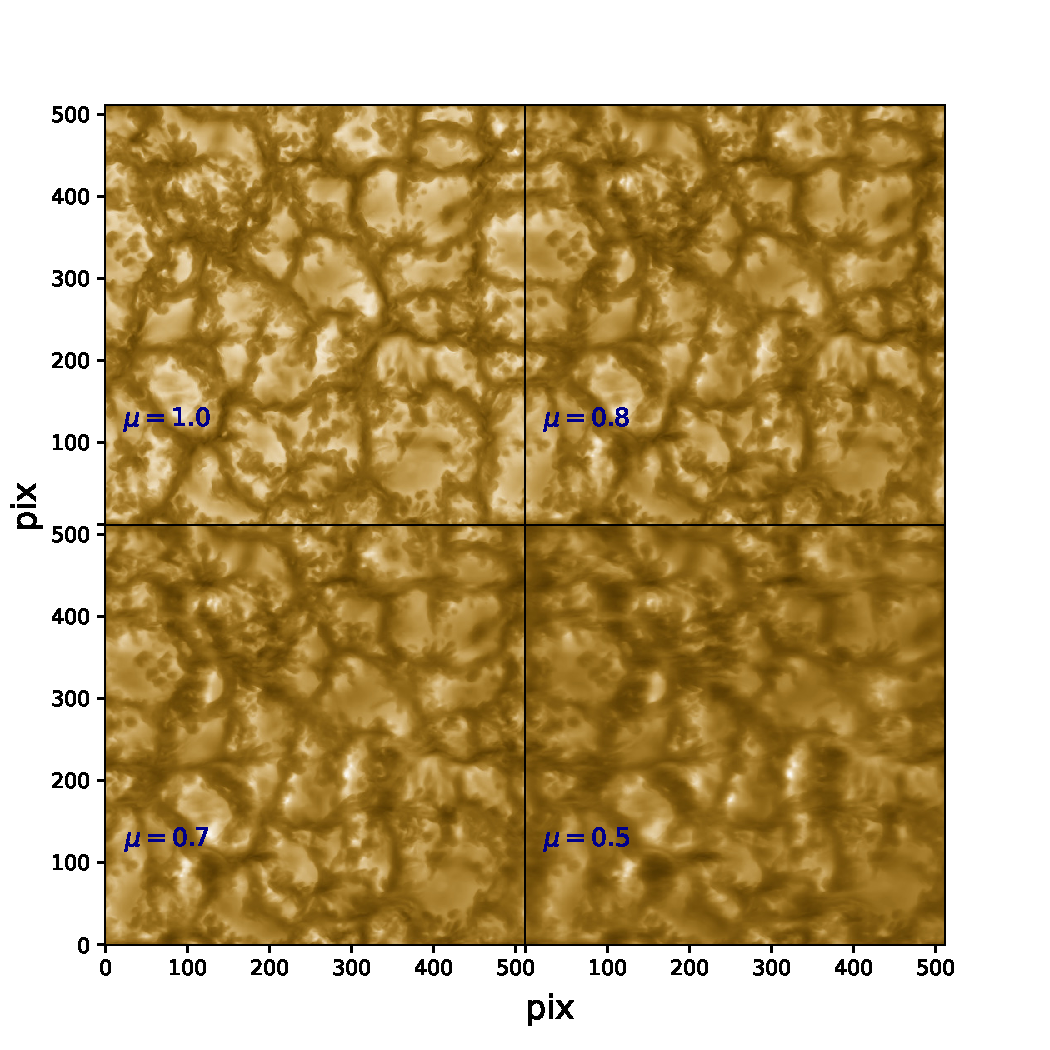
\includegraphics[width=.4\textwidth]{mps.pdf}
        \caption{Forward modeled intensity maps at various $\mu$ values for BB2 filter of SUIT.}
    \label{fig:flux_maps}
\end{wrapfigure}
%%%%%%%%%%%%%%%%%%%%%%

We use 3D MHD model atmospheres simulated by \cite{rempel20} and 1.5D RT with MPS-ATLAS \citep[see e.g.,][for details]{anusha21} with measured filter profiles of {\suit}, to calculate the emergent intensity. The 3D MHD simulation employs a symmetric lower boundary condition for the magnetic field and a variety of initial magnetic field configurations to create small-scale variations and various levels of magnetization. The RT equation is solved using the method of ODFs, accounting for both continuum and line opacities within the concerned wavelength range. This takes into account both continuum and line opacity within the concerned wavelength range. Accurately accounting for the line opacity is one of the major challenges in synthesizing spectra over a broad wavelength range. In the ODFs method, the opacity is sorted without the information of the corresponding wavelength within small intervals of wavelengths known as bins. The geometric mean of the sorted opacity values for multiple sub intervals within a given wavelength bin is pre-tabulated over atmospheric parameters such as temperature, pressure and micro-turbulent velocities. During RT calculations, opacity is then interpolated for the required grid parameters of the atmospheric model. The primary goal of the ODF method is to significantly minimize the computational time required for RT calculations. This becomes particularly crucial when computing emergent spectra across numerous atmospheres, such as those arising from 3D MHD simulations. 
%
\chapter{Stellar calibration of SUIT}\label{c:chap5}
\chaptermark{SUIT stellar calibration}
\begin{quote}
{\em ~~~~~~~This thesis chapter originally appeared in the literature as} \\
{authors,
{\em journal reference info}}
\end{quote}
%\begin{abstract}

 %   The  \ion{Mg}{2}~k \& h line intensity ratios can be used to probe the characteristics of the plasma in the solar atmosphere. In this study, using the observations recorded by the Interface Region Imaging Spectrometer (IRIS), we study the variation of the  \ion{Mg}{2}~k \& h intensity ratio for three flares belonging to X-class, M-class, and C-class, throughout their evolution. We also study the k-to-h intensity ratio as a function of magnetic flux density obtained from the line-of-sight magnetograms recorded by the Helioseismic and Magnetic Imager (HMI) on board the Solar Dynamics Observatory (SDO). Our results reveal that while the intensity ratios are independent of magnetic flux density, they show significant changes during the evolution of the C-class and M-class flares. The intensity ratios start to increase at the start of the flare and peak during the impulsive phase before the flare peak and decrease rapidly thereafter. The values of the ratios fall even below the pre-flare level during the peak and decline phases of the flare. These results are important in the light of heating and cooling of localized plasma and provide further constraint on the understanding of flare physics.
    
%\end{abstract}
\justifying

%%----------------------------------------------------
\section{Introduction} \label{sec:intro}
%%----------------------------------------------------

Solar flares are the most energetic events on the Sun, where an enormous amount of magnetic free energy is released due to the reconfiguration of the coronal magnetic field. The released energy can cause particle acceleration, heating and flows in the solar atmosphere and a transient enhancement in solar radiative output. Notably, a significant portion of the radiated energy during flares originates from the dense chromosphere \citep{fletcher10,milligan14}. Therefore, examining chromospheric lines during flares offers valuable diagnostic tools for understanding the physics of solar flares and their impact on the local plasma environment.

The chromosphere emits radiation across various ultraviolet (UV) and optical lines. While many optical lines, such as H$\alpha$ and \ion{Ca}{2}, are routinely observed from ground-based telescopes, observations of the  \ion{Mg}{2} resonance lines have been relatively infrequent in the past. However, since the launch of the Interface Region Imaging Spectrograph (IRIS) \citep{iris}, regular monitoring of these lines with excellent spatial and spectral resolution has become possible.

The  \ion{Mg}{2} k and h lines represent transitions to the ground state from finely split upper levels ($3p~^{2}P_{\nicefrac{3}{2}}${--}$3s~^{2}S_{\nicefrac{1}{2}}$ and $3p ^{2}P_{\nicefrac{1}{2}}${--}$3s^{2}S_{\nicefrac{1}{2}}$), resulting in optically thick lines at wavelengths 2796.34~{\AA} ( \ion{Mg}{2} k) and 2803.52{\AA} ( \ion{Mg}{2} h). It has been suggested that the intensity ratios of these lines can offer insights into the optical depth of the local environment \citep{kerr15}.

The integrated intensity of a line transitioning from an upper level $j$ to a lower level $i$ depends on the collision strength $\Omega_{ij}$ for that transition, given by~\citep{henri62,mariska92},

%%---------------------------------------------------------------
\begin{equation*}
\Omega_{ij}=\frac{8\pi}{\sqrt{3}}~\frac{I_{H}}{\Delta \epsilon_{ij}}g\omega_{i}~f_{ij}
\end{equation*}
%%---------------------------------------------------------------

\noindent Here, $I_{H}$ denotes the ionization energy of hydrogen, $\Delta \epsilon_{ij}$ represents the threshold energy for the transition, $g$ is the Gaunt factor, $\omega_{i}$ is the statistical weight of the level, and $f_{ij}$ stands for the oscillator strength. In optically thin conditions, the intensity ratio of the k to h line equals the ratio of collision strengths, as the escape probability of photons is unity. As the  \ion{Mg}{2} k and h lines share the same ionization state and originate from a transition to a shared lower level, and given that the statistical weight ($\omega_{i}$) is the same in both cases, the line intensity ratio is simply the ratio of oscillator strengths ($f_{ij}$). Consequently, this ratio is expected to be 2:1 in optically thin conditions and lower when the medium is optically thick \citep{kerr15,levens19}.

Moreover, the  \ion{Mg}{2} k and h lines can serve to estimate velocity in the middle and upper chromosphere, chromospheric velocity gradients, and temperature in the middle chromosphere \citep{leenarts13a,leenarts13b,pereira13}. Emission from the  \ion{Mg}{2} triplets can help identify heating in the lower chromosphere \citep{pereira15}. Various studies have demonstrated spatial variations in  \ion{Mg}{2} line profiles \citep{dalda23,panos18}. For instance, \cite{polito23} associated the leading edge of flare ribbons with enhanced broadening and strong central reversal, interpreting this difference in profile as indicative of distinct heating mechanisms at different locations within flare ribbons. Similarly, \cite{panos21,panos21_2} revealed differences in line profiles and energy input.

Using observations recorded by the OSO-8 LPSP instrument, \citep{lemaire84} investigated the evolution of intensity ratios of  \ion{Mg}{2} h \& k, \ion{Ca}{2} h \& k, and Ly$\alpha$ \&~$\beta$ lines. They observed that the intensity ratio of the \ion{Ca}{2}~k/h lines increased from 1 to 1.2 during the ascending phase of a flare and returned to 1 during later phases. This correlated temporal behavior across various elements was interpreted as an indication of downward energy propagation, suggesting a potential decrease in opacity due to localized heating at the formation height of the \ion{Ca}{2} line during the flare's rise phase.

Here, we investigate the evolution of intensity ratios of the  \ion{Mg}{2} h \& k lines during three flares: C-class, M-class, and X-class. Specifically, we focus on the dependence of line ratios on the underlying magnetic field strength, a relationship that, to our knowledge, has not been explored previously. The remainder of this chapter is organized as follows. Section \ref{sec:obs} presents the observations utilized in this study, followed by our data reduction and analysis methods, and the results in Section \ref{sec:dar}.

%%----------------------------------------------------
\section{Observations} \label{sec:obs}
%%----------------------------------------------------
%%-------------------------------------------------------
\begin{table*}[ht!]
\centering
\begin{tabular}{|c|c|c|c|c|c|}
\hline
Event & Flare & Flare & Raster & Raster Step & Raster \\
Date & Peak (UT) & Location (arcsec) & Details & (arcsec) & Cadence (s)\\
\hline
Nov 4, 2015  & 13:52 & [37",61"] & Coarse & 2" & 50\\
(M-class) & & & 16-step  & & \\
 & & & & & \\
Oct 22, 2014 & 14:28 & [-292",-302"] & Coarse & 2" & 131\\
(X-class) & & & 8-step  & & \\
 & & & & & \\
Feb 3, 2015 & 22:55 & [198",213"] & Dense & 0.35" & 33\\
(C-class) & & & 16-step  & & \\
\hline
\end{tabular}%}
%\end{center}
\caption{List of flares studied in this chapter.}
\label{tab:my_label}
\end{table*}
%%-------------------------------------------------------

For this study, we selected three flares of M, X, and C classes, as listed in Table~\ref{tab:my_label} by IRIS. IRIS is a NASA small explorer-class solar observation satellite that obtains UV spectra with high spatial (0.33{--}0.4\arcsec per pixel), temporal (1s), and spectral resolution ($\sim$26 and $\sim$53~m{\AA}). The primary lines regularly observed by IRIS include \ion{C}{2},  \ion{Mg}{2}, and \ion{Si}{4}. In the imaging channel, it typically observes in  \ion{Mg}{2} and \ion{Si}{4}. In our study, we utilized observations recorded in the  \ion{Mg}{2} h\& k lines.

As mentioned earlier, this study aims to analyze the evolution of intensity ratios concerning magnetic flux density during the flares of various classes. To achieve this, we incorporated line-of-sight (LOS) magnetic field measurements from the Helioseismic and Magnetic Imager \citep[HMI;][]{hmi} on the Solar Dynamics Observatory \citep[SDO;][]{sdo}. We utilized observations taken at 1600~{\AA} by the Atmospheric Imaging Assembly \citep[AIA;][]{aia}, also onboard SDO, to co-align the IRIS observations with those from AIA and subsequently HMI.

%%----------------------------------------------------
\section{Data analysis and results} \label{sec:dar}
%%----------------------------------------------------
\subsection{M3.7 Flare Observed on Nov 4, 2015}
%%%----------------------------------------------
%%--------------------------------------------------

NOAA AR 12443 generated a multi-ribbon GOES class M3.7 flare on November 4, 2015, which commenced around 13:31 UT and peaked at approximately 13:52 UT, as observed from the GOES Soft X-ray (SXR) 1{--}8~{\AA} flux (Fig.\ref{flare1}a). This event occurred at approximately [37\arcsec,61\arcsec] heliographic position and was extensively observed by IRIS, AIA, and HMI. Fig.\ref{flare1}a illustrates the GOES flux plot of the flare in the 0.5{--}4~{\AA} range (blue) and the 1.0{--}8.0~{\AA} range (red). Fig.\ref{flare1} b depicts AIA 1600{\AA} image of the flaring region, showing two ribbons indicated by arrows. In panel (c), we present the line-of-sight (LOS) magnetic flux density map obtained from HMI, recorded nearly simultaneously with the AIA image shown in panel (b). The white (black) box overlaid on Fig.\ref{flare1}(b) (c) represents the IRIS SJI (Slit-Jaw Imager) field of view (FOV). The white dot-dashed (magenta dashed) box in Fig.\ref{flare1}b (c) indicates the IRIS raster FOV. The FOV of the SJI (approximately [120\arcsec~$\times$119\arcsec]) covers the central part of the flaring region, with a spectral sampling of approximately 0.05~{\AA}/pixel. \cite{li17} investigated the dynamics of the ribbons for this flare, while \cite{karlick18} studied the associated radio bursts.

%%--------------------------------------------------
\begin{figure*}[ht!]
    \centering
\includegraphics[trim={7cm 5cm 7.7cm 6cm},clip,width=\textwidth]{Figures/Flare_M_Nov04_2015_2.eps}
\caption{The M3.7 flare observed on November 4th, 2015. Panel a: GOES flux plot in 0.5{--}4~{\AA} (blue) and 1.0{--}8.0~{\AA} (red). Panel b: AIA 1600~{\AA} image of the flaring region. Arrows locate the primary ribbons. Panel c: LOS magnetic flux density map obtained from HMI near the peak of the flare. The over-plotted white (black) boxes in panel b (c) represent the IRIS SJI FOV. The over-plotted white dot-dashed (magenta dashed) box in panel b (c) shows the IRIS raster FOV.}\label{flare1}
\end{figure*}
%%--------------------------------------------------

Figure~\ref{flare_m_ev} illustrates the evolution of the flare in AIA 304~{\AA}. The flare is connected with a pre-existing filament that undergoes an eruption, splitting into two structures denoted as F1 \& F2 in Fig.\ref{flare_m_ev}(b) \& (c). These two filament structures diverge from each other in opposite directions. The flare generates two primary flare ribbons, labeled as R1 \& R2 in Fig.\ref{flare_m_ev}(b), (c) \& (d). Starting around 13:32 UT, R1 travels southeastward, crossing the IRIS raster FOV, indicated by the white dotted box in Fig.\ref{flare_m_ev}(a), (b), (c) \& (d). The IRIS raster monitors the movement of the northern ribbon R1 and the eastern edge of R2. An animated version of Fig.\ref{flare_m_ev} is available in the online journal for further details.

%%%--------------
\begin{figure*}[ht!]
    \begin{center}
    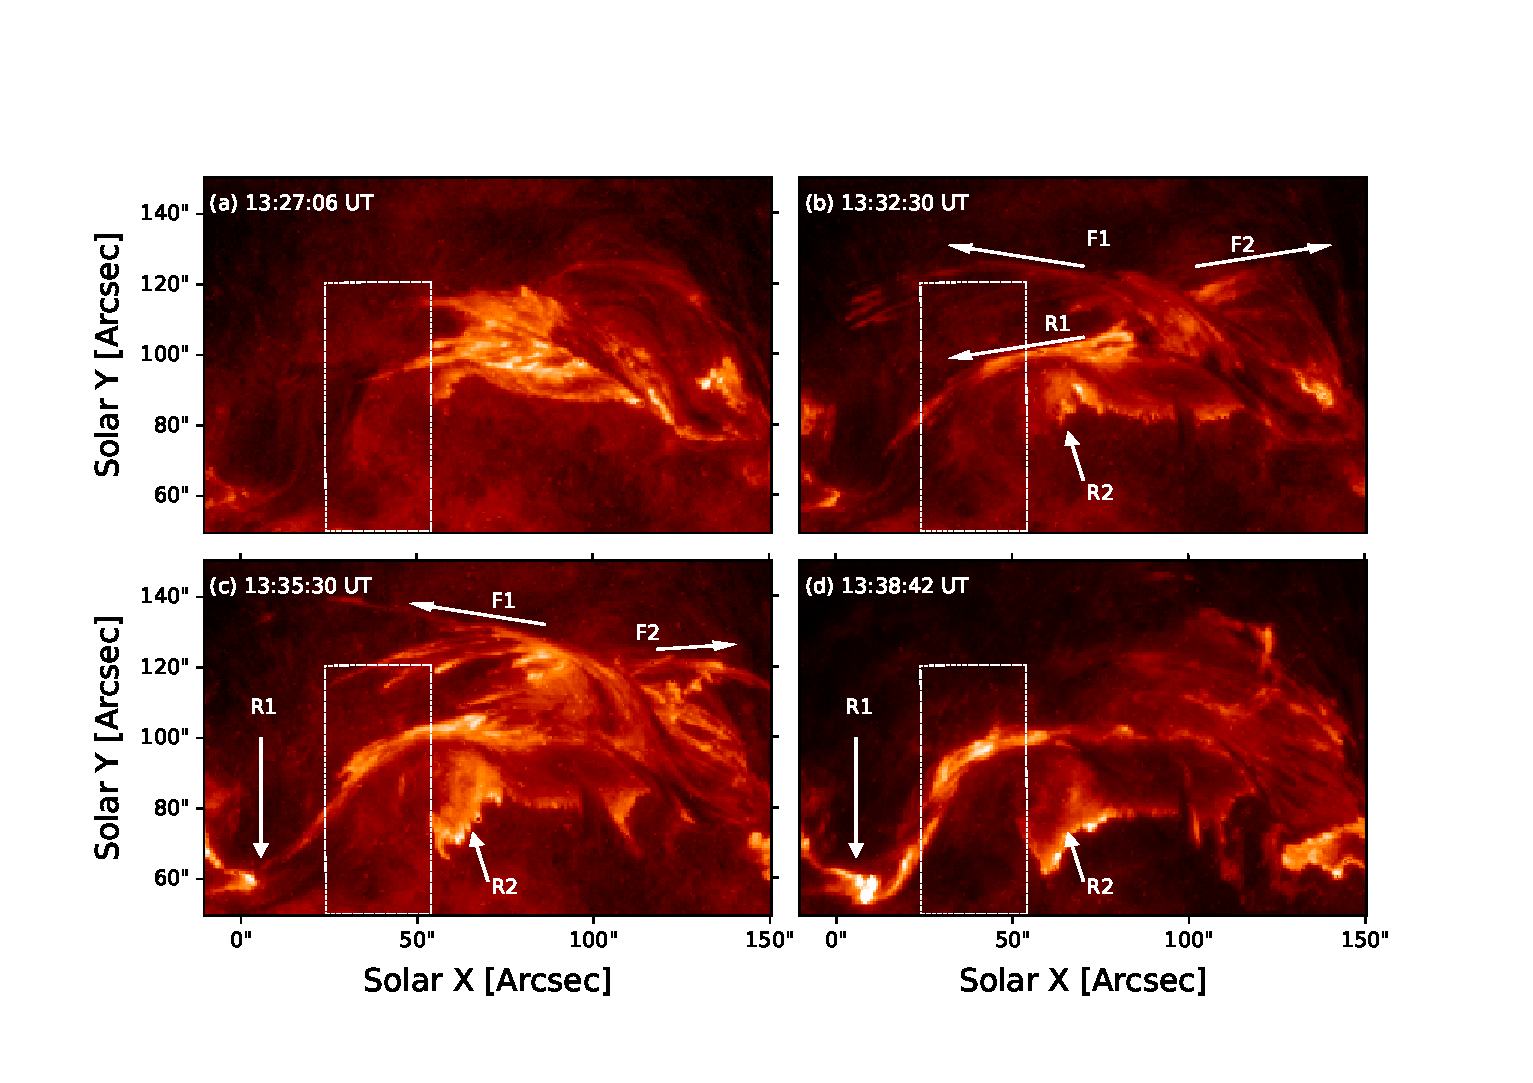
\includegraphics[width=\textwidth]{Figures/nov_flare_304_aa_evolv.eps}
    \end{center}
    \caption{Sequence of AIA 304~{\AA}~images for the Nov 4th, 2015 flare. The white dotted box shows the portion of the IRIS raster FOV which scanned the ribbons. In panels b (c) F1 and F2 are the filament material, which move away from each other as the flare progresses. R1 and R2 in b (c,d) show the primary ribbons which move through the IRIS raster FOV. An animation of this image sequence is available in \cite{roy24}.}
    \label{flare_m_ev}
\end{figure*}
%%%--------------

Fig.\ref{flare_m_aia} presents the same region as depicted in Fig.\ref{flare_m_ev} across the six coronal channels (i.e., 94, 131, 171, 193, 211, 335~{\AA}) of SDO/AIA, recorded at the peak (top two rows) and during the decline phase (bottom two rows) of the flare. Post-eruption arcades \citep[][]{TriBC_2004} are clearly observable in all the channels, displaying slightly varied morphologies. These arcades contain evaporated thermal plasma and exhibit loop top brightening, likely due to colliding evaporation flows \citep[see, e.g.,][]{sharma16, patsourakos04}.

%%%--------------
\begin{figure*}[ht!]
    \begin{center}
        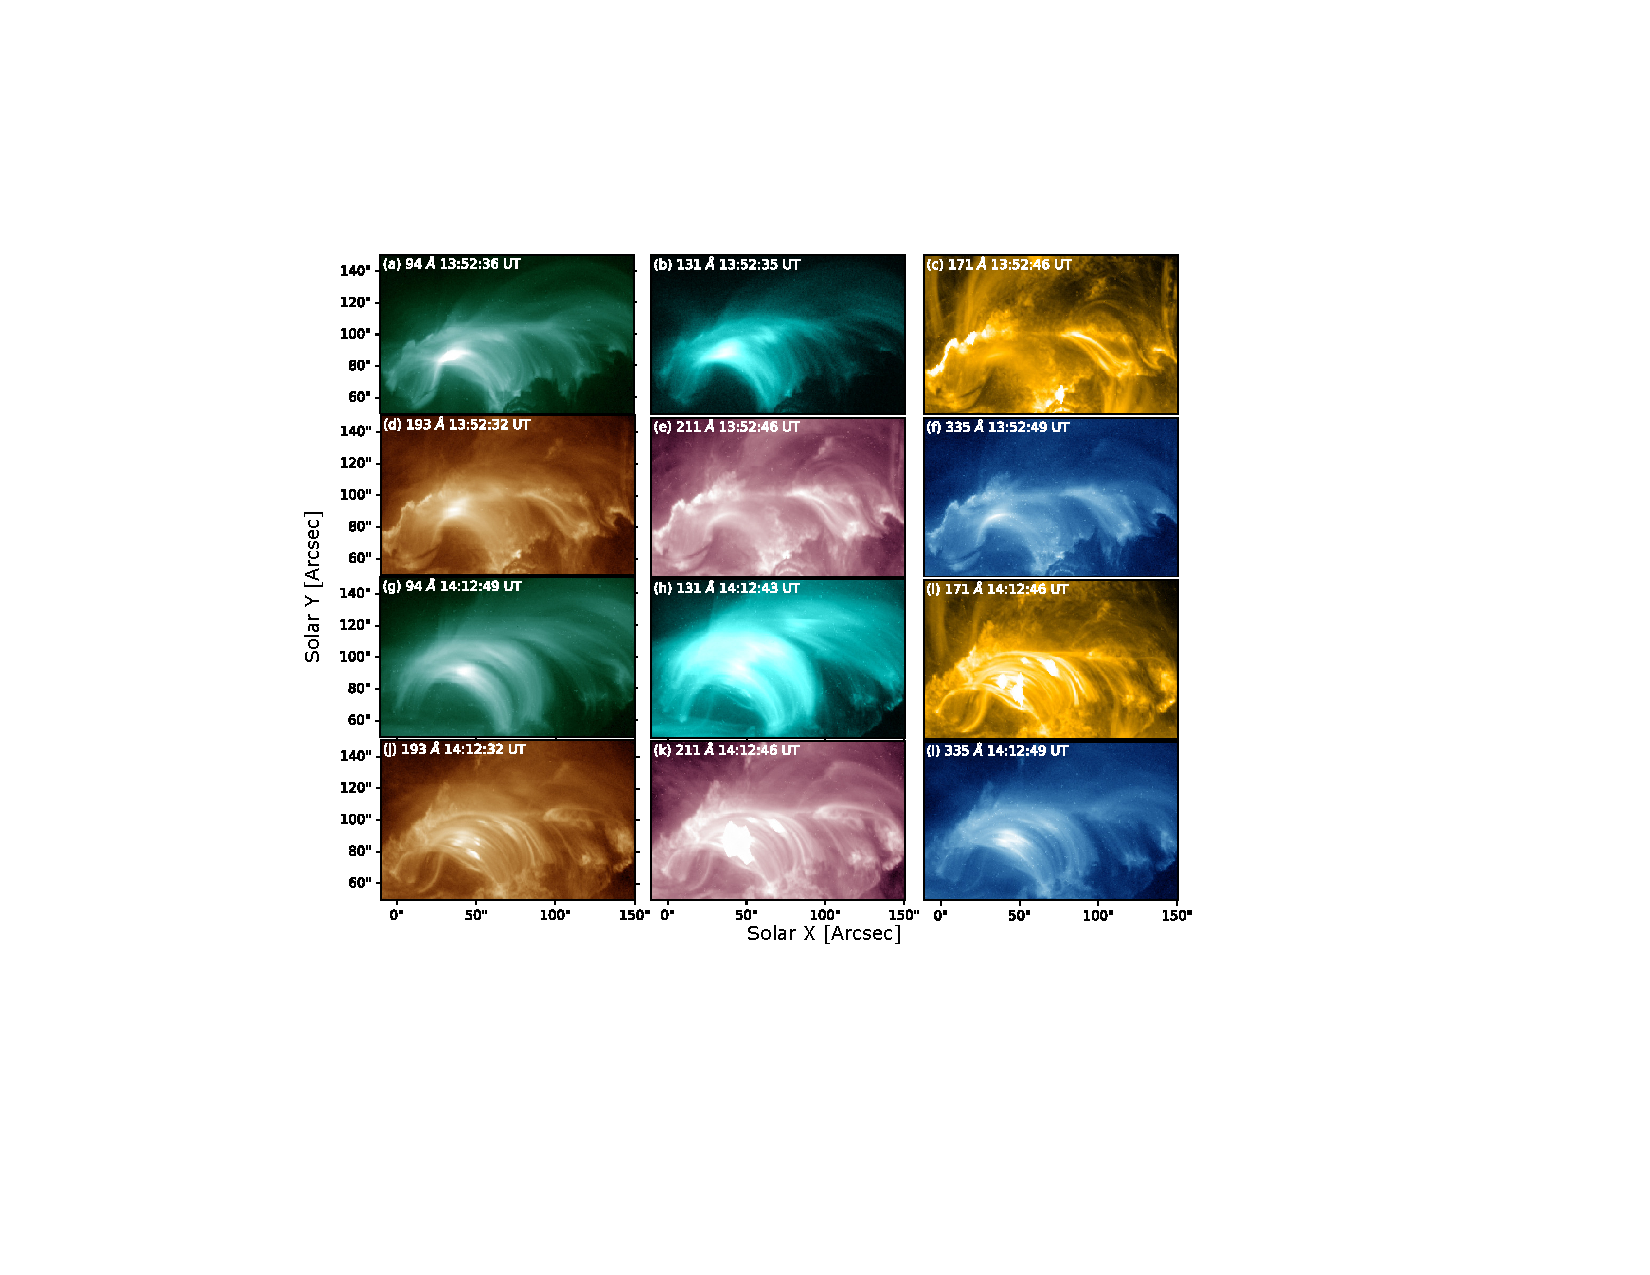
\includegraphics[trim={4.5cm 5.5cm 6cm 4cm},clip,width=\textwidth]{Figures/nov_flare_aia_waves_2.pdf}
    \end{center}
    \caption{The Nov 4th, 2015 flare in the six Coronal channels of the SDO/AIA at the soft X-ray peak (panels (a)-(f)) and during the decline phase (panels (g)-(l)) of the flare.}
    \label{flare_m_aia}
\end{figure*}
%%%--------------

We begin by aligning the HMI observations with the IRIS observations using the 1600~{\AA} data recorded by AIA. Given that the observation involves an active region undergoing flaring, the magnetic field may also be rapidly changing \citep{wang02,dandan16,spirock02}. Therefore, we utilize a series of co-aligned full-disk maps from AIA and HMI to derive a rastered line-of-sight (LOS) map of magnetic flux density that precisely corresponds to the location and time of IRIS rasters. This procedure is outlined below.

Initially, we align the AIA 1600~{\AA} observation with the HMI observation closest in time to the IRIS SJI (Slit-Jaw Imager) and raster observations. Using the `aia\_prep' tool available in the \textit{sswidl} distribution, we process the level 1 images to perform image registration and align AIA and HMI observations. Subsequently, we calculate the shift between AIA 1600~{\AA} and the SJI 1400~{\AA}. Using these calculated offsets, we co-align the magnetograms with the IRIS SJI 1400~{\AA} observations, given that the AIA 1600~{\AA} observation was already aligned with the HMI observations. We typically observe an offset of approximately $\sim$ 1.5\arcsec~between HMI and IRIS. These co-aligned HMI maps are then utilized to derive the rastered magnetograms, which can be directly compared with IRIS raster observations.

%%%%-------------------------
\begin{figure}[ht!]
\centering  
\vspace{10cm}
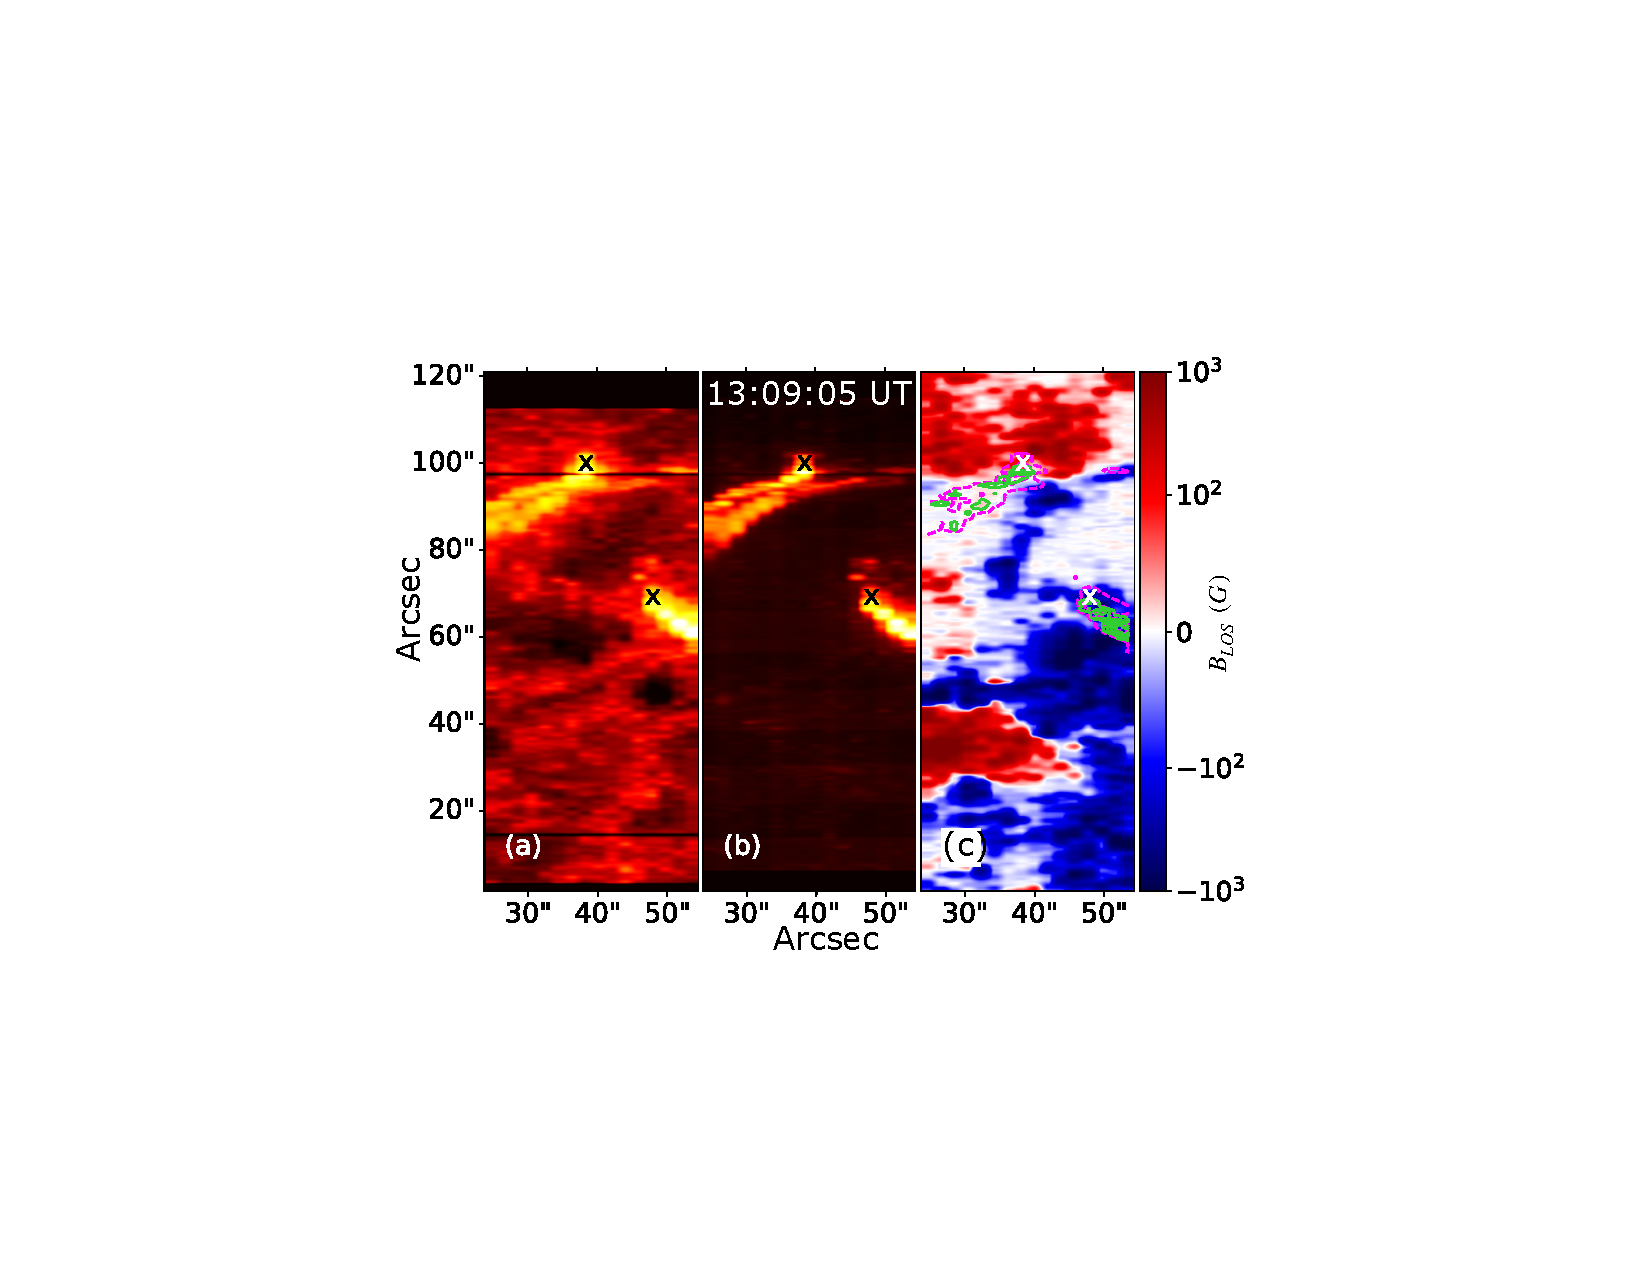
\includegraphics[trim={7cm 5cm 6cm 15cm},width=0.7\textwidth]{Figures/m_flare_iris.pdf}
\caption{Obtained images in  \ion{Mg}{2} h (panel a) and k (panel b) and corresponding co-aligned and artificially rastered HMI LOS magnetic field map (panel c) for the M3.7 flare observed on November 4th, 2015. The magenta and lime green contours on panel c show the contours of  \ion{Mg}{2}~h (panel a) and k (panel b) intensity.} \label{fig:aligned_raster}
\end{figure}
%%%%-------------------------

For analyzing the properties of the  \ion{Mg}{2} lines, we fit a double Gaussian profile to both the k and h lines with a linear background symmetric about the line core. If excess emission is detected compared to the fitted background and line profile for wavelengths lower than 2792~{\AA} and in-between 2798~{\AA} to 2800~{\AA}, we infer the presence of  \ion{Mg}{2} triplets in emission. A single Gaussian profile is fitted to the excess emission. It's important to note that this approach may overlook the triplets unless the emission is sufficiently strong. However, this method serves our purpose since our primary objective is to characterize the  \ion{Mg}{2} k and h line profiles.

Additionally, we exclude any pixels showing saturation in either of the lines. The uncertainty of the observed intensities is measured in DN (Data Numbers) using the method outlined in \S2.1 of \cite{kerr15} and subsequently applied in the fitting procedure. The uncertainties of the fitted Gaussian profiles are incorporated while integrating the profile to obtain the uncertainty of the line intensities.

%%%%%%%%%%%
\begin{figure*}[ht!]
    \centering
    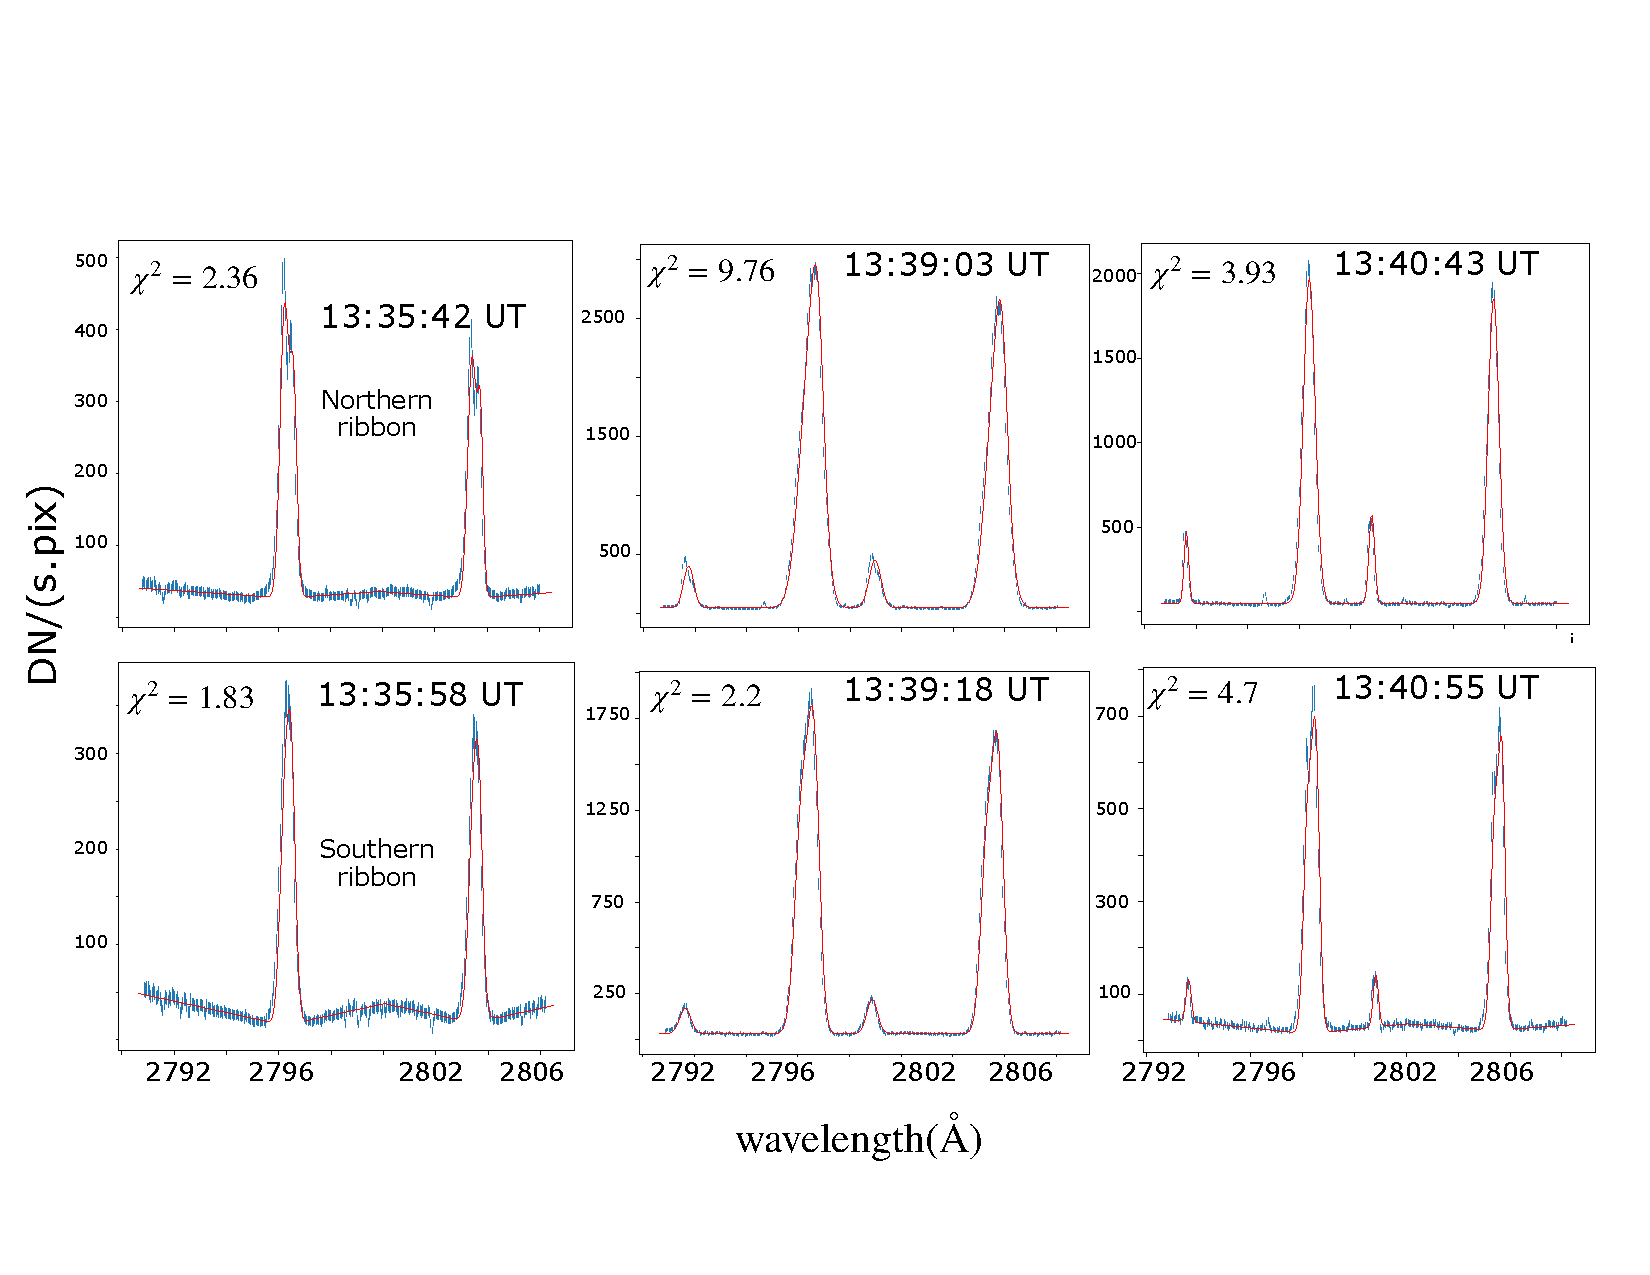
\includegraphics[trim={0cm 3cm 0.5cm 3cm},clip,width=\textwidth]{Figures/pix_fit.pdf}
    \caption{Fit of the  \ion{Mg}{2} window for the pixel marked in northern ribbon (southern ribbon) in Fig.~\ref{fig:aligned_raster} in top panel (bottom panel) from various times during the evolution of the flare. }
    \label{fig:pix_fit_ribbon}
\end{figure*}
%%%%%%%%%%%

%%%%-------------------------
\begin{figure}[ht!]
\centering  
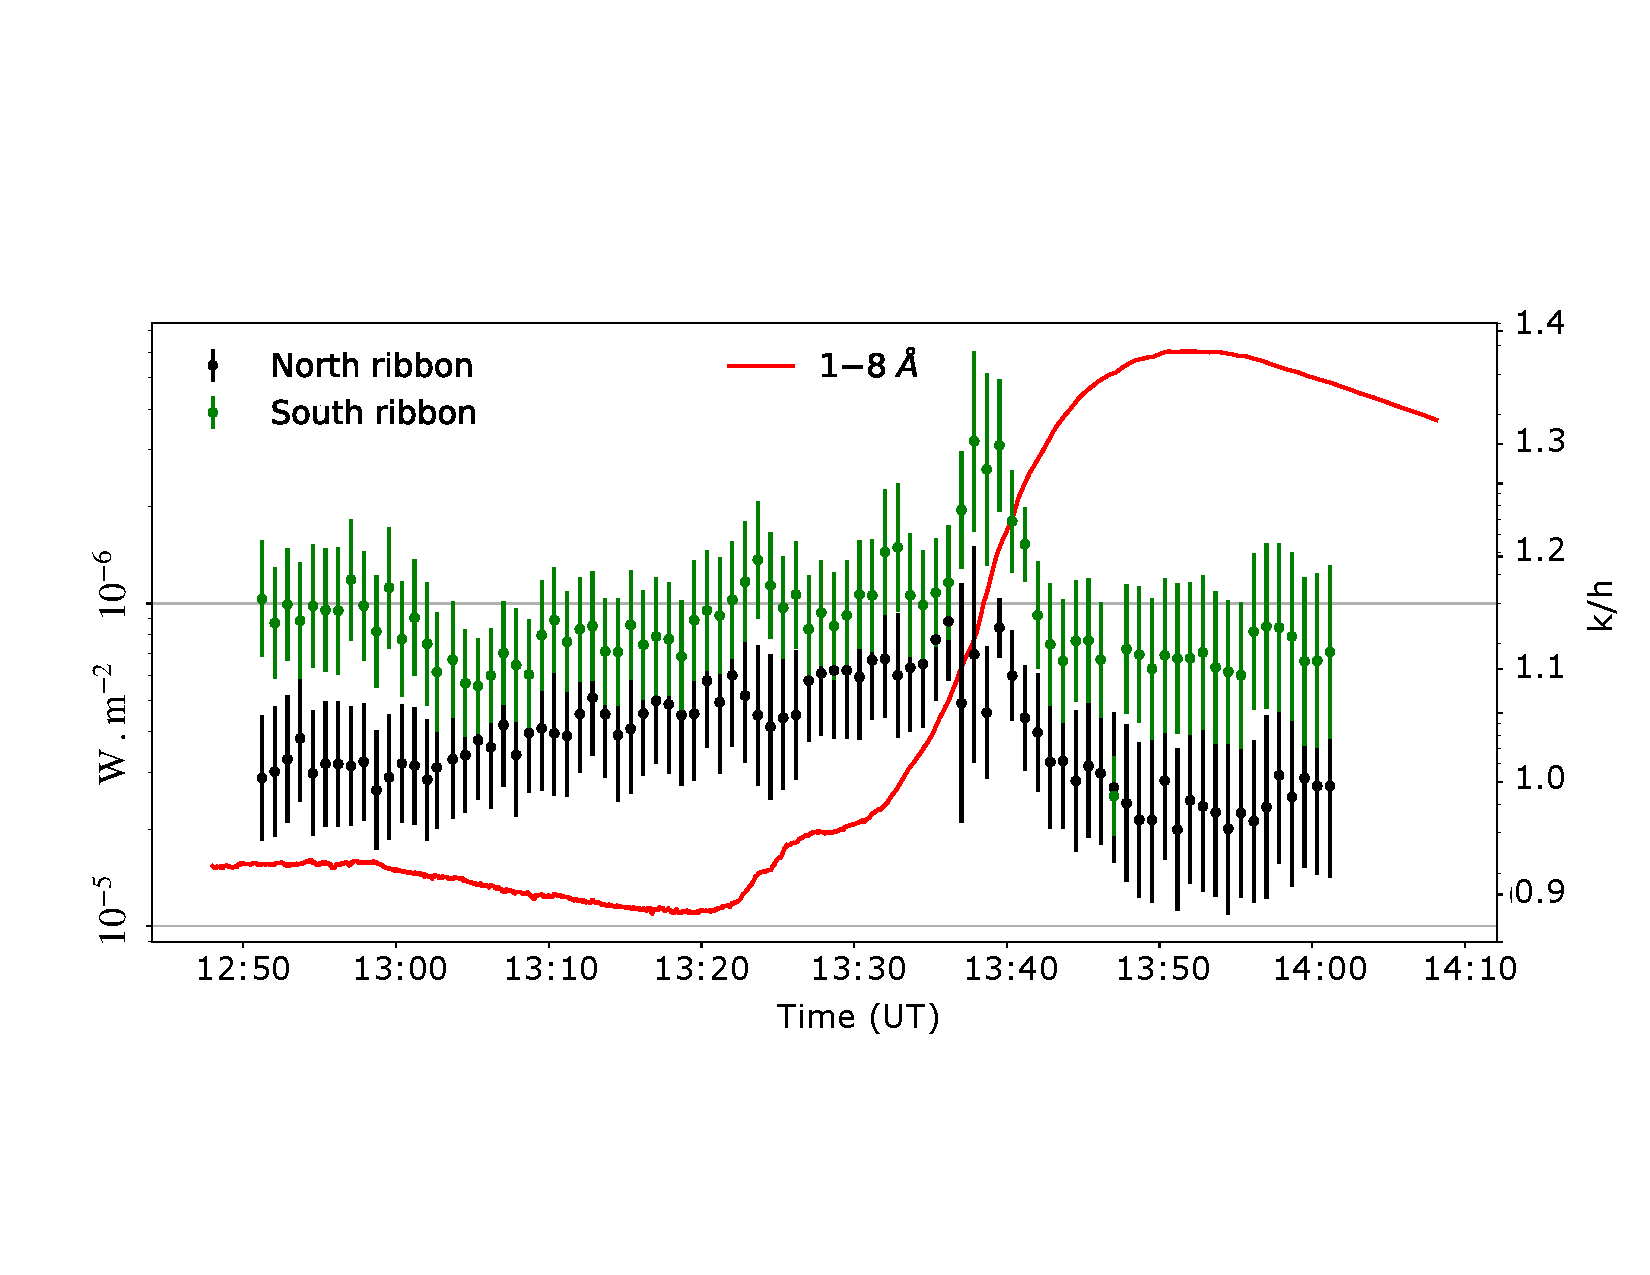
\includegraphics[trim={1.5cm 4cm 0.5cm 4cm},clip,width=0.8\textwidth]{Figures/m_flare_iris_pt2.pdf}
\caption{The 1{--}8~{\AA} GOES light curve of the flare over-plotted with the time variation of  \ion{Mg}{2} k/h line intensity ratio for the northern (black) and southern (green) asterisks marked in panels a, b \& c.}
\label{fig:aligned_iris_ratio}
\end{figure}
%%%%-------------------------

In Figure~\ref{fig:aligned_raster}, we present intensity maps obtained in  \ion{Mg}{2} h \& k (panels a \& b) alongside the rastered line-of-sight (LOS) magnetic field map in panel (c). The dashed magenta and solid green contours on the magnetic field maps represent the intensity from panels a and b, respectively. To investigate the  \ion{Mg}{2} k to h intensity line ratios over time, we selected two pixels—one in the northern ribbon and another in the southern ribbon, as indicated by crosses. Fig.~\ref{fig:pix_fit_ribbon} displays the spectra overlaid with fits for the two pixels taken in the northern ribbon (top panel) and southern ribbon (bottom panel) obtained at different times.

We illustrate the  \ion{Mg}{2} k to h line intensity ratio derived from the two locations in the northern (black) and southern ribbons (green) in Fig.\ref{fig:aligned_iris_ratio}. Additionally, we overlay the GOES light curve of the flare obtained in 1.0{--}8.0{\AA} (red solid line). Our observations indicate that the intensity ratios exhibit a slightly increasing trend, albeit within the margin of errors, during the early phase of the flare. The ratio demonstrates a distinct peak around the midpoint of the impulsive phase, lasting for a very brief duration of approximately 150 seconds, before beginning to decrease. It's worth emphasizing that the pixel-by-pixel fitting of the  \ion{Mg}{2} h \& k line profiles provided a sufficient signature of the time evolution of the k/h line intensity ratio during the flare.

%%%%%%%--------%%%%%%%%%%%
\subsection{Investigating the dependence on the local magnetic field in the  \ion{Mg}{2} lines}
%%%%%%%---------%%%%%%%%%%

To explore the time evolution of the intensity ratio and its potential relationship with the photospheric magnetic field, we binned the spectra into various magnetic field bins from different flaring pixels. We selected the flaring pixels based on an intensity threshold relative to the peak intensity observed in IRIS rasters. A double Gaussian fit with a constant background was performed in a smaller wavelength window for both the  \ion{Mg}{2} h and k lines separately. This step was essentially carried out to mitigate the effects of the background and potential contributions from other spectral features.

Fig.~\ref{fig:fit_pix_fov} displays the  \ion{Mg}{2} k line profiles obtained at different times and averaged over different magnetic field bins. Each plot denotes the observation time and the magnetic field strength over which the spectra were averaged and fitted with a double Gaussian. Line intensities were computed by integrating the fitted Gaussian.

In Fig.~\ref{fig:optical_depth_m}, we present the k to h intensity ratios obtained in various bins of magnetic flux density at different times corresponding to different flare phases. The curve corresponding to 13:07:05 UT (red) represents the pre-flare phase, where the ratio is approximately 1.2. The ratio shows an increase during the impulsive phase, i.e., the curves corresponding to 13:23:44 UT (blue dotted) and 13:32:04 UT (green dashed). The ratio measured at 13:41:11 UT (magenta dashed), which is closest to the UV peak of the flare, exhibits the largest value across all magnetic field bins. Subsequently, during the decline phase, the ratio measured at 13:57:23 UT (black solid) falls below the values observed during the pre-flare phase. Additionally, it's noteworthy that there are no significant differences among the k to h ratios obtained in different bins of magnetic flux density at all times (including pre-flare, impulsive, peak, and decline phases) of the flare.

%%%%-----------------------
\begin{figure*}[ht!]
    \begin{center}
    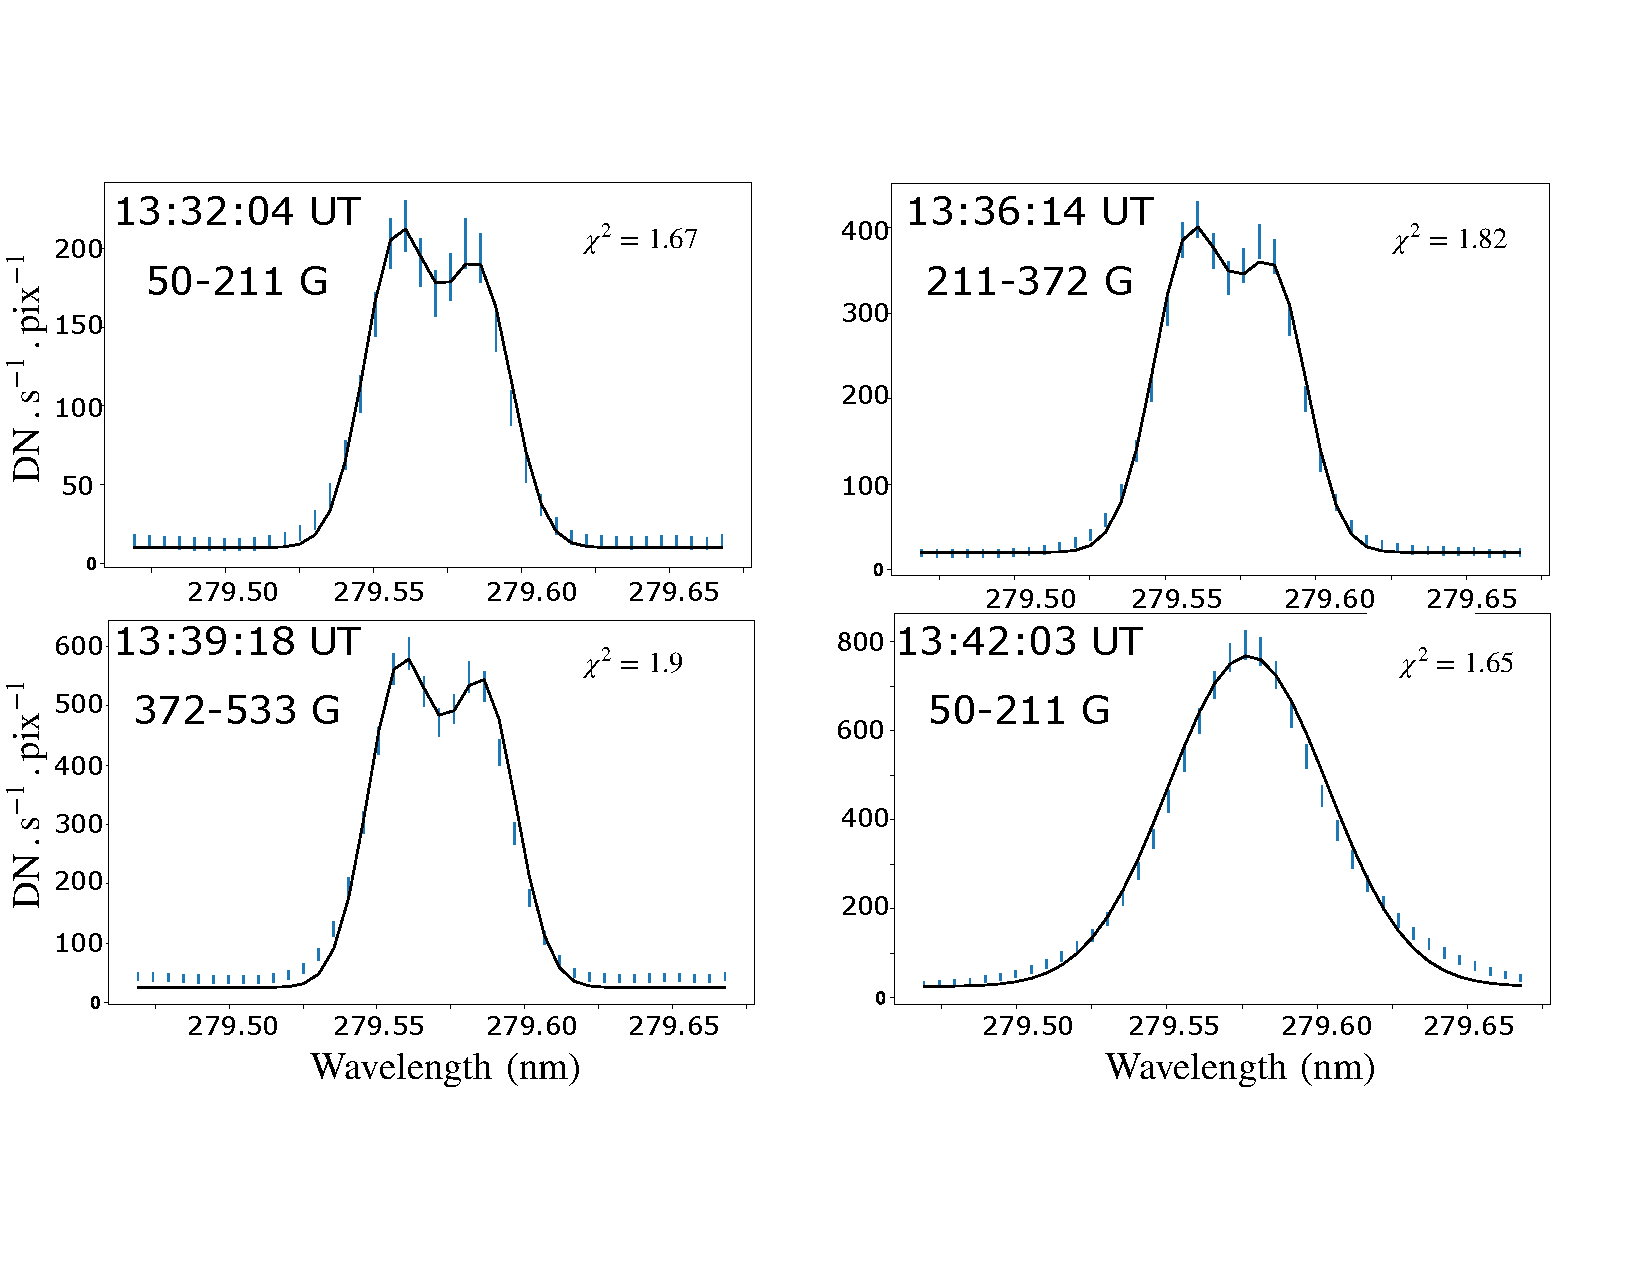
\includegraphics[trim={0cm 3cm 0cm 3cm},clip,width=\textwidth]{Figures/binned_fit_fov.pdf}
    \end{center}
    \caption{Fitted line profiles for the binned spectra for various magnetic field strengths from various times.}
    \label{fig:fit_pix_fov}
\end{figure*}
%%%%----------------------- 

%%----------------------------------------------------------------------------
\begin{figure}[ht!]
    \centering
    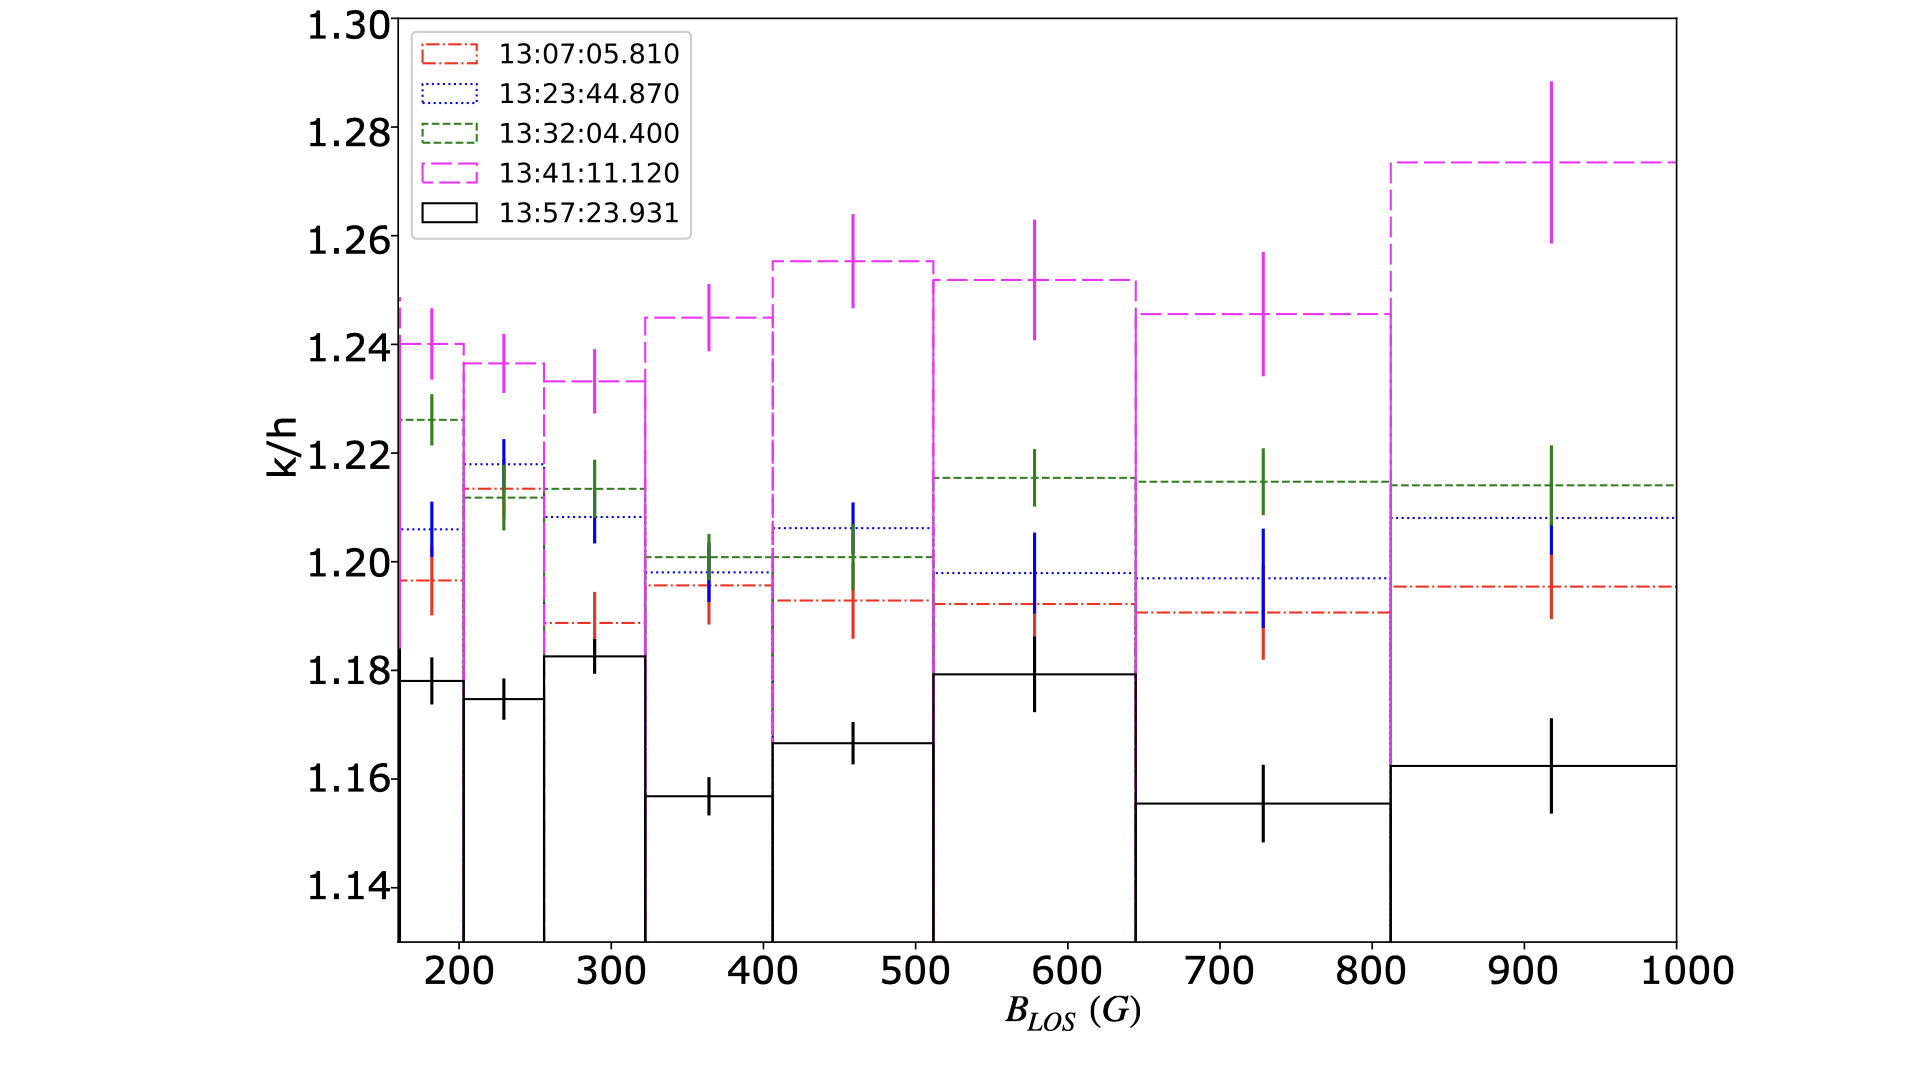
\includegraphics[trim={8cm 1cm 2cm 0.2cm},clip,width=0.9\textwidth]{Figures/Flare-m-optical-depth-2.jpeg}
    \caption{ \ion{Mg}{2} k to h line intensity ratio for various magnetic flux density bins at various time steps during the evolution of the flare.}
    \label{fig:optical_depth_m}
\end{figure}
%%----------------------------------------------------------------------------

To explore further, we study the evolution of k to h intensity ratio as a function of time during the flare. In Fig.~\ref{fig:optical_dep_ev_m}, we plot the time evolution of the k to h line intensity ratio averaged within the bins of different magnetic flux densities as a function of time. For better visibility the 20.9{--}184.4 G and 348.9{--}513.3 G points are offset by 30s and -30s, respectively. We also plot the GOES 1{--}8~{\AA} light curve with the red solid line. These plots conspicuously reveal that the intensity ratios rise sharply during the impulsive phase, from $\sim$ 1.20 to $\sim$ 1.28 right before the soft X-ray flux peaks as seen from GOES, and decreases very rapidly thereafter, to lower than pre-flare values $\sim$ 1.12. The typical uncertainty value for the line intensity ratio is $\sim$ 0.02. We further note that the evolution of the  \ion{Mg}{2} k to h intensity ratio is remarkably similar across various strengths of magnetic flux densities.

%%%----------------------------------------------
\begin{figure*}[ht!]
    \centering
    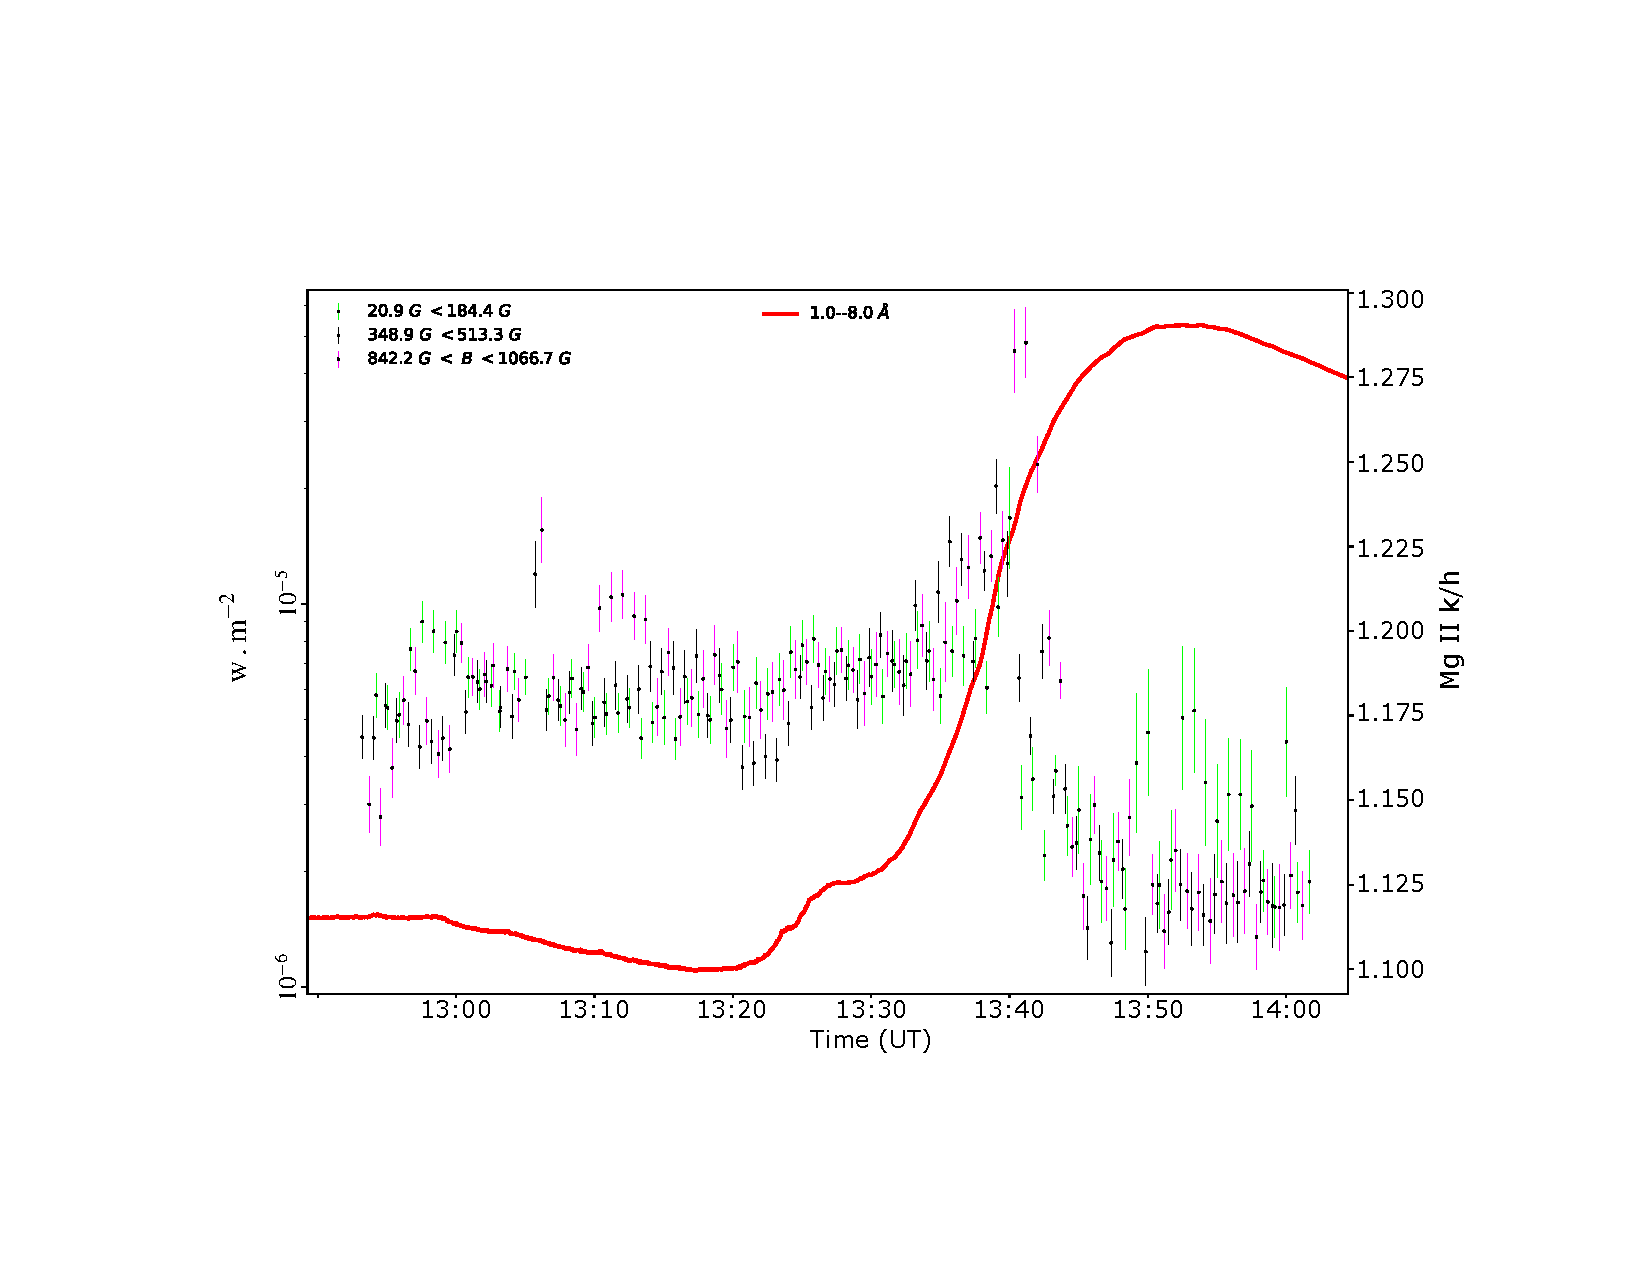
\includegraphics[trim={3cm 3cm 2cm 4cm},clip,width=\textwidth]{Figures/Nov-11-2015-optical-dep-ev-5.pdf}
    \caption{Time evolution of the  \ion{Mg}{2} k to h line intensity ratio obtained from averaged spectrum over the corresponding magnetic flux bin as labeled for the Nov 4, 2015 flare. For better visibility, the 20.9{--}184.4 G and 348.9{--}513.3 G points are offset by 30s and -30s respectively. Over-plotted red solid line displays the 1{--}8~{\AA} GOES X-ray light curve.}
    \label{fig:optical_dep_ev_m}
\end{figure*}
%%%----------------------------------------------

%%%----------------------------------------------
\subsection{X1.6 Flare Observed on Oct 22, 2014}
%%%----------------------------------------------

An X~1.6 flare occurred on October 22, 2014, observed in AR 12192. The flare commenced at 14:02 UT and peaked at 14:28 UT as observed by GOES. Fig.\ref{flare2}(a) illustrates the GOES flux plot of the flare in the 0.5{--}4~{\AA} range (blue) and the 1.0{--}8.0~{\AA} range (red). Figs.\ref{flare2}(b) \& (c) display an AIA 1600{\AA} image and the line-of-sight (LOS) magnetic flux density map obtained from HMI, respectively. The overlaid boxes in panels (b) and (c) indicate the IRIS SJI (Slit-Jaw Imager) field of view (FOV). IRIS observed this flare with a large 8-step coarse raster covering a FOV of [14\arcsec,174\arcsec]. It's worth noting that the IRIS SJI FOV and the slit direction were rotated by approximately 45$^\circ$ relative to the center of the HMI observation.

%%--------------------------------------------------
\begin{figure}[ht!]
    \centering
\hspace*{-.5in}
\includegraphics[width=\textwidth,trim={7cm 5cm 7.7cm 6cm},clip]{Figures/Flare_X_oct22_2014_2.eps}
\caption{The X class flare observed on October 22, 2014. Panel a: GOES flux plot in 0.5{--}4~{\AA} (blue) and 1.0{--}8.0~{\AA} (red). Panel b: AIA 1600~{\AA} image taken at the peak of the flare. Arrows locate the primary and secondary ribbons. Panel c: LOS magnetic flux density map obtained from HMI at the peak of the flare. The over-plotted white (black) box in panel b (c) represents the IRIS SJI FOV, and white dot-dashed (dashed) box in panels b (c) represents the IRIS Raster FOV.}\label{flare2}
\end{figure}
%%--------------------------------------------------

The flare manifests two ribbons in AIA 1600{\AA}, as indicated by the arrows. The eastern ribbon extends around a negative field region and is entirely covered by the IRIS SJI FOV. Conversely, the western ribbon extends around a positive field region, with only a portion of it covered by the IRIS SJI FOV, as depicted in panel (b). In Fig.~\ref{fig:align_raster_flare2}, we present intensity maps obtained in  \ion{Mg}{2} h \& k (panels a \& b) alongside the rastered line-of-sight (LOS) magnetic field map (panel c). The black \& green dashed contours in the LOS magnetic field map (panel c) indicate the intensity contours of  \ion{Mg}{2} h \& k (panels a \& b).

%%--------------------------------------------------
\begin{figure}[ht!]
    \centering
%    \hspace{2in}
    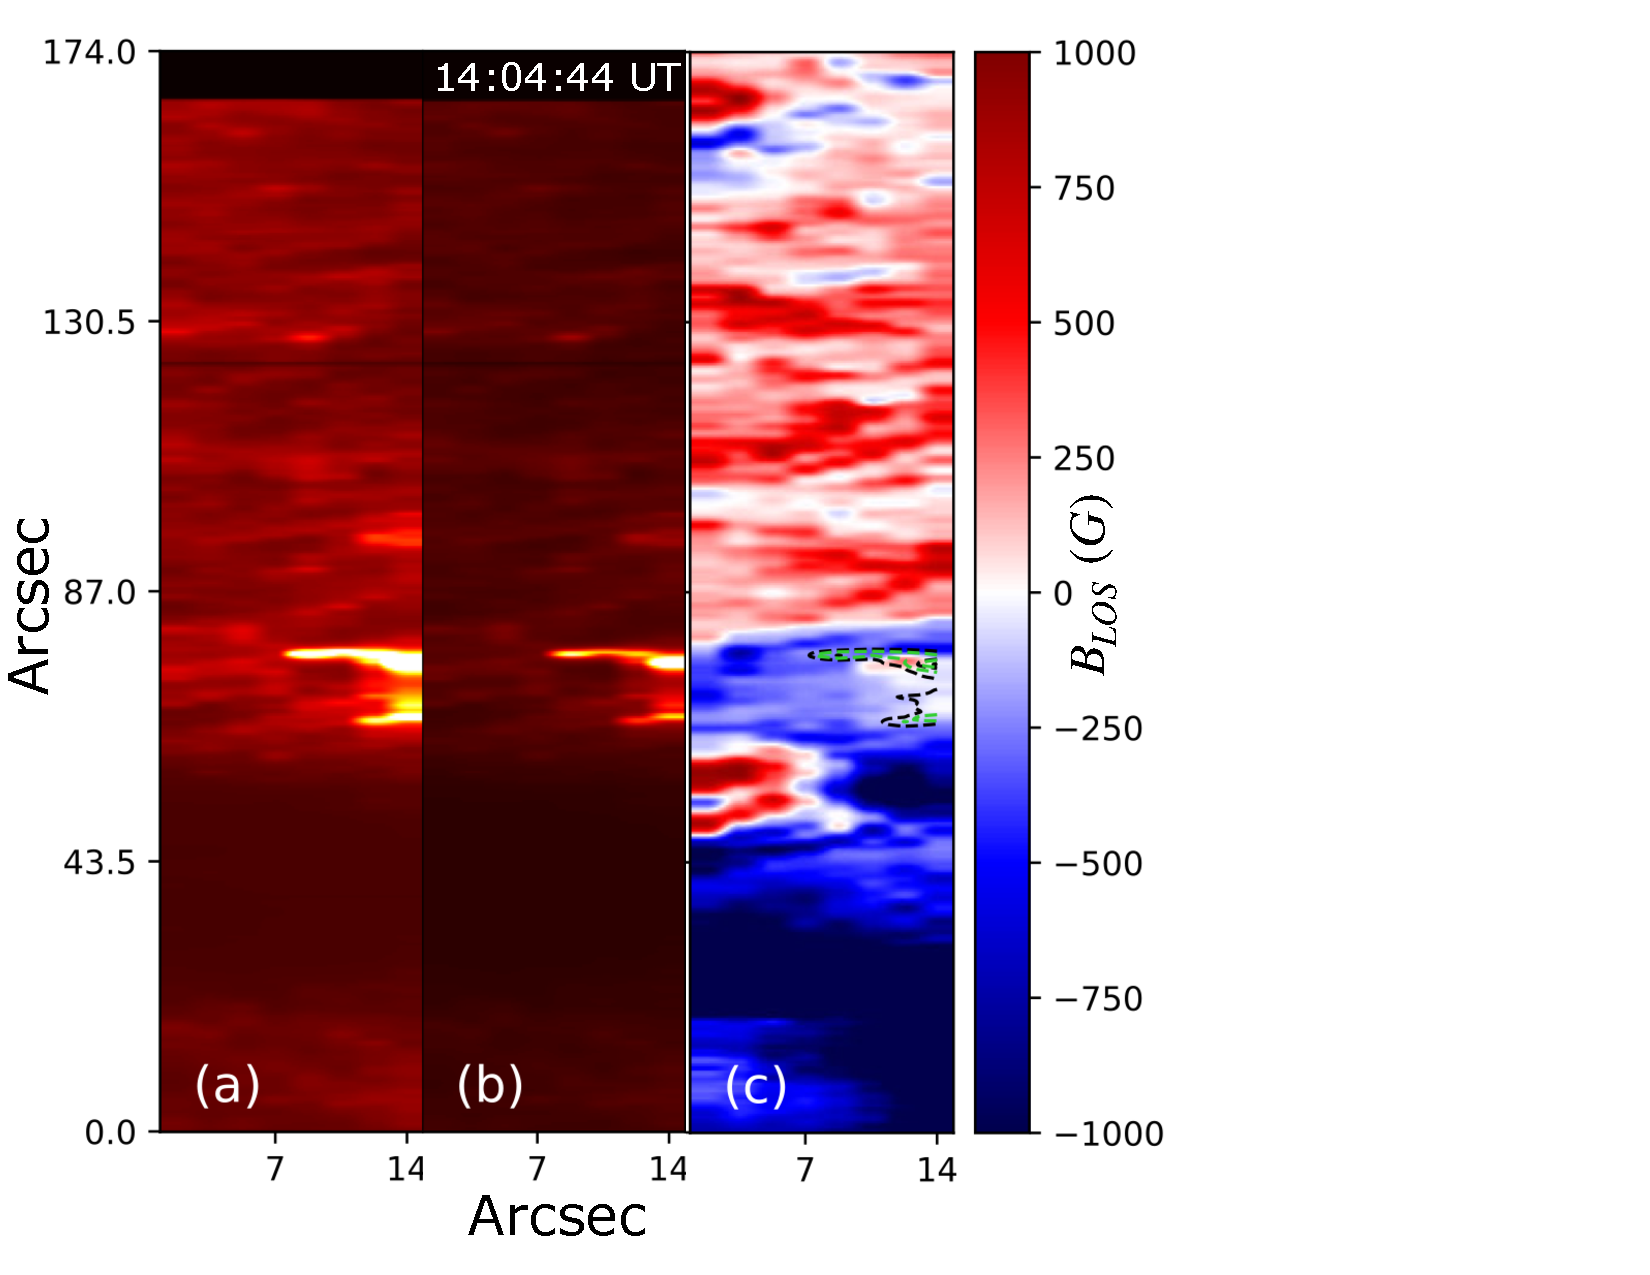
\includegraphics[trim={6cm 3cm 6cm 3cm},clip,width=0.45\textwidth]{Figures/contour_paper_plot_oct28.pdf}
    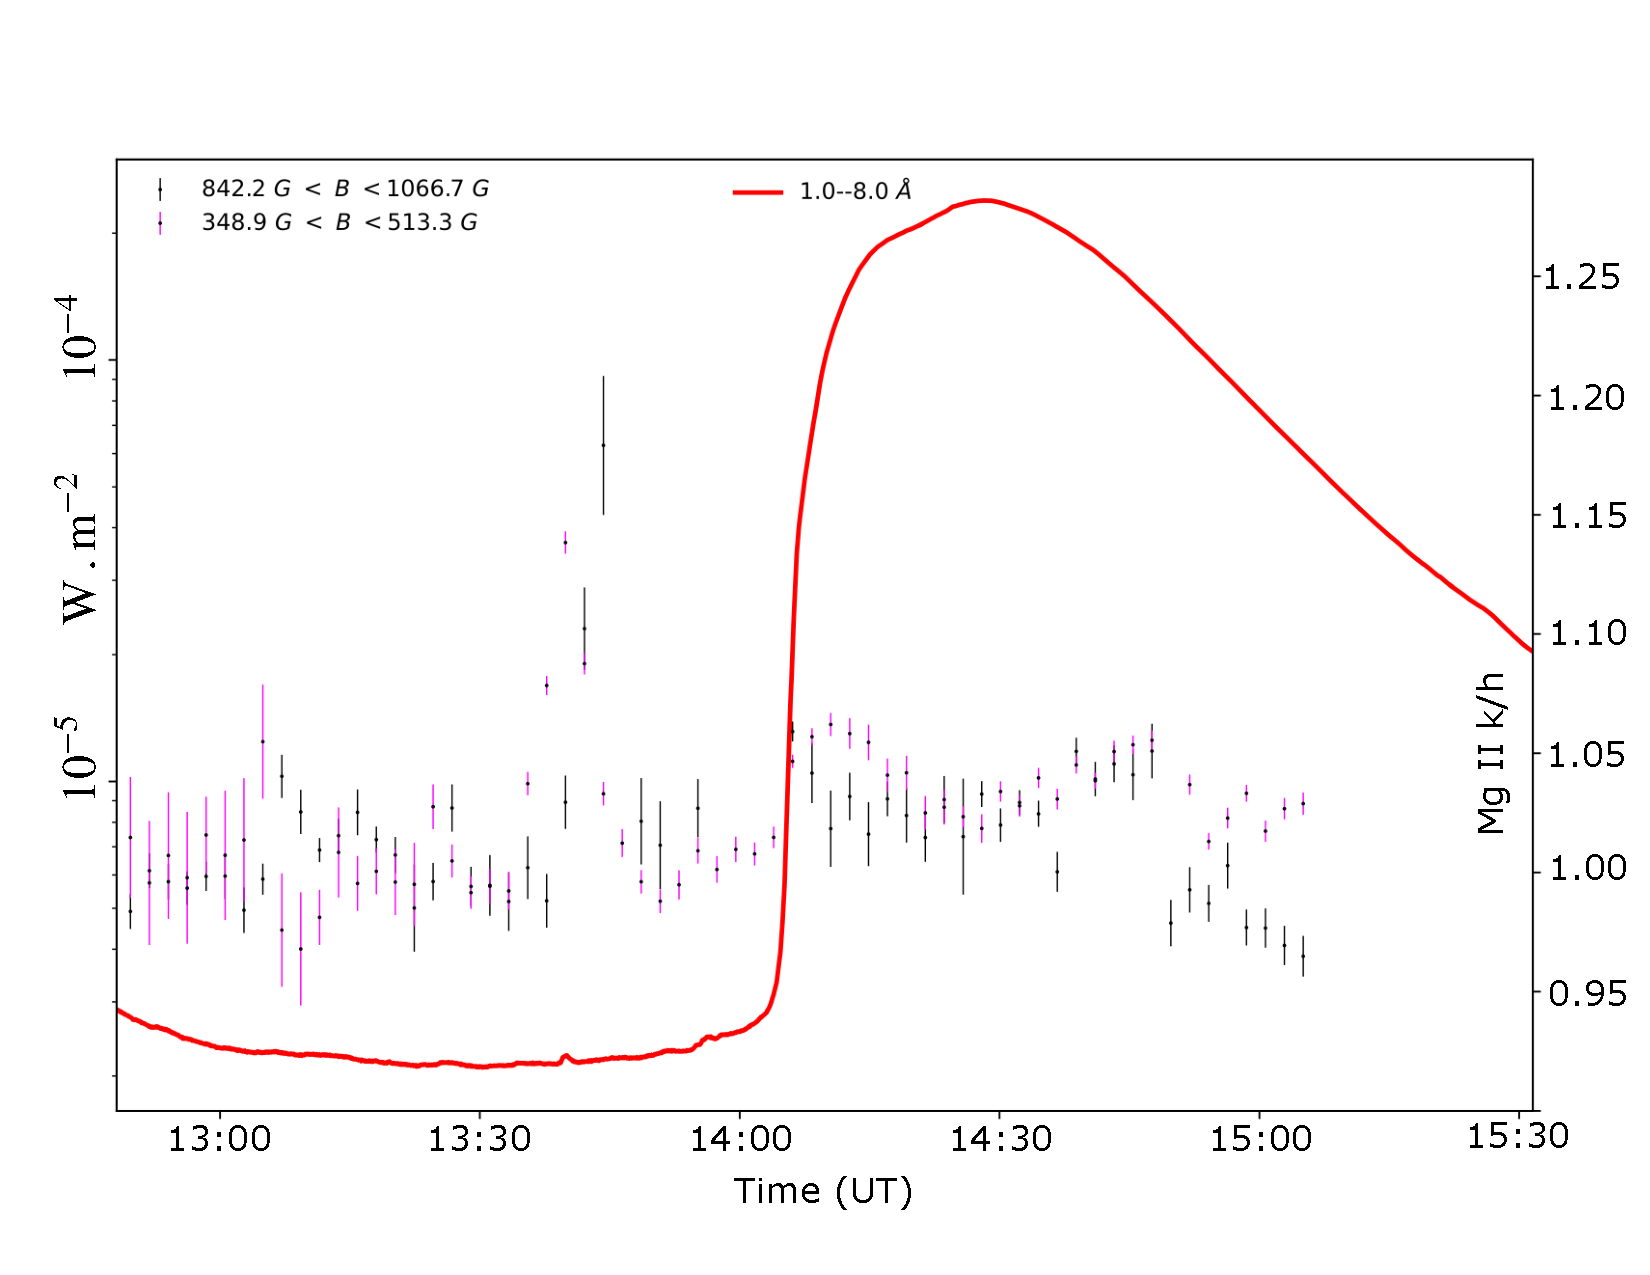
\includegraphics[trim={3cm 2cm 2cm 3cm},clip,width=0.45\textwidth]{Figures/Oct-22-2014-optical-dep-ev-2.pdf}
    \caption{Obtained intensity maps in  \ion{Mg}{2}~k (panel a) and h (panel b) lines at the peak of the flare. The rastrered HMI LOS magnetic field density map is shown in panel c. The black and lime green contours on panel c show the contours of  \ion{Mg}{2}~k (panel a) and h (panel b) intensity.}
\label{fig:align_raster_flare2}
\end{figure}
%%--------------------------------------------------

Similar to the M-class flare studied in the previous section, we derive the  \ion{Mg}{2} k to h line intensity ratio for various bins of the magnetic flux density within the flaring region and study their time evolution. In Fig.\ref{fig:align_raster_flare2} right panel, we plot the intensity ratio in black and magenta colors for two different magnetic field bins. In the same panel, we also overlay the 1{--}8~{\AA} GOES light curve (red solid line). We note that, unlike the M-class flare, we do not observe any noticeable change in the intensity ratio during the flare. There are approximately two to three data points showing an enhancement in the ratio, but these occur well before the onset of the flare.

%%%----------------------------------------------
\subsection{C3.5 Flare Observed on Feb 03, 2015}
%%%----------------------------------------------

On February 3, 2015, AR 12277 generated a C-class flare that peaked at 22:55 UT. Fig.\ref{flare3} depicts the GOES flux plot of the flare in the 0.5{--}4{\AA} range (blue) and the 1.0{--}8.0~{\AA} range (red) in panel (a). Fig.\ref{flare3}(b) \& (c) displays an AIA 1600{\AA} image and the line-of-sight (LOS) magnetic flux density map obtained from HMI, respectively, recorded near the peak of the flare.

The overlaid white (black) box in panel (b) ((c)) indicates the IRIS SJI (Slit-Jaw Imager) field of view (FOV). The over-plotted white dot-dashed (magenta dashed) box in panel (b) ((c)) indicates the IRIS raster FOV. IRIS observed this flare with a large dense 16-step raster with a FOV of 5"$\times$119" and a step size of 0.35\arcsec. The flare exhibits a double ribbon structure, with the east ribbon elongating earlier and merging into the west ribbon. The IRIS raster scans through the west edge of the west ribbon through its eruption and merging with the east ribbon. Fig.~\ref{fig:align_raster_flare3} displays the intensity maps obtained in  \ion{Mg}{2} h \& k (panels a \& b). The rastered LOS magnetic field map is shown in panel (c). The black \& green dashed contours in the LOS magnetic field map (panel c) depict the intensity contours of  \ion{Mg}{2} h \& k (panels a \& b).

%%--------------------------------------------------
\begin{figure*}[ht!]
    \centering
\hspace*{-.6in}
\includegraphics[width=1.12\textwidth,trim={7cm 5cm 7.7cm 6cm},clip]{Figures/Flare_C_feb03_2015_2.eps}
%\includegraphics[width=.7\textwidth]{figures/Feb_03_2015/Feb-04-2015-optical-dep-ev-2.eps}
\caption{The C class flare observed on February 3rd, 2015. Panel a: GOES flux plot in 0.5{--}4~{\AA} (blue) and 1.0{--}8.0~{\AA} (red). Panel b: AIA 1600~{\AA} image of the flaring region. Panel c: LOS magnetic flux density map obtained from HMI near the peak of the flare. The over-plotted white (black) boxes in panel b (c) represents the IRIS SJI FOV. The over-plotted white dot-dashed (magenta dashed) box in panel b (c) show the IRIS raster FOV.}\label{flare3}
\end{figure*}
%%--------------------------------------------------

%%--------------------------------------------------
\begin{figure}[ht!]
    \centering
%\hspace*{-1.in}
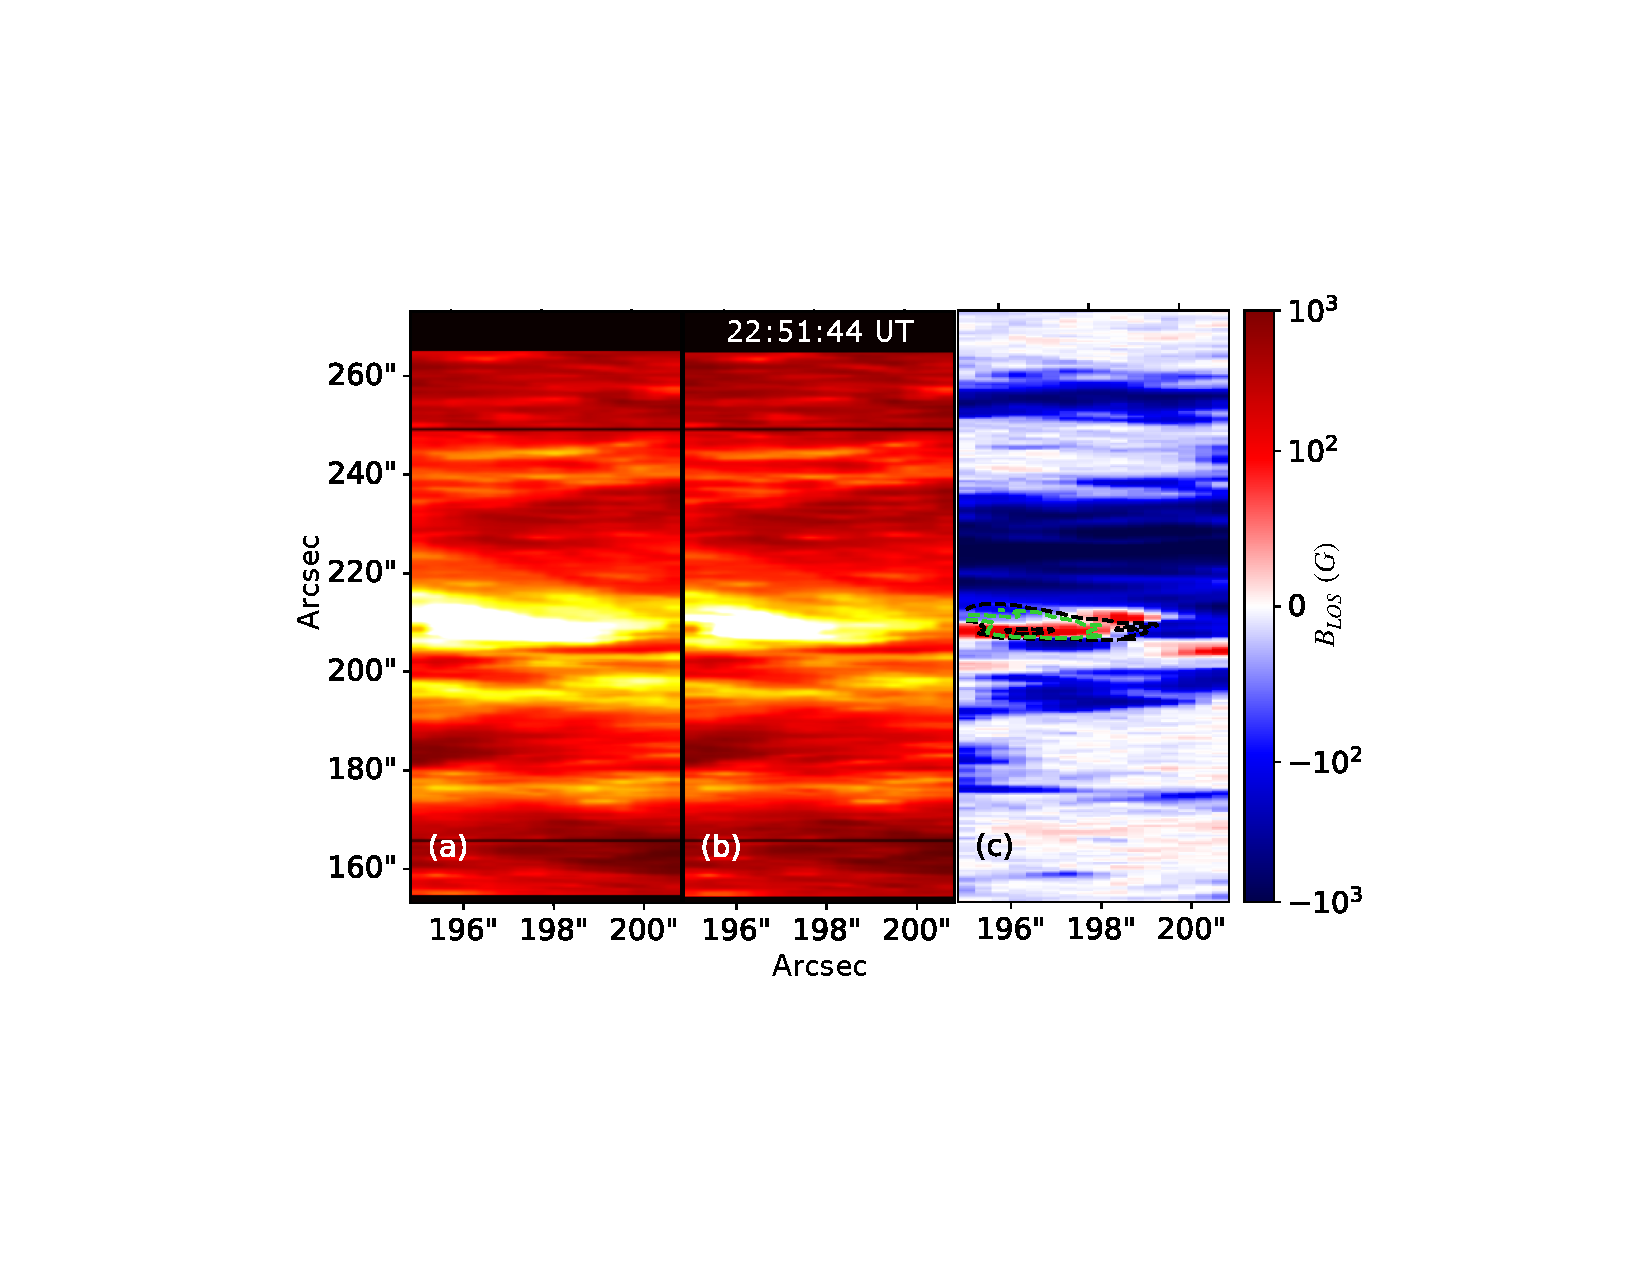
\includegraphics[width=0.5\textwidth,trim={4cm 5cm 4cm 4cm},clip]{Figures/contour_paper_plot_feb-03-2015.pdf}
\caption{Obtained intensity maps in  \ion{Mg}{2}~k (panel a) and h (panel b) lines at the peak of the flare. The rastrered HMI LOS magnetic field density map is shown in panel c. The black and lime green contours on panel c show the contours of  \ion{Mg}{2}~k (panel a) and h (panel b) intensity.}
\label{fig:align_raster_flare3}
\end{figure}
%%--------------------------------------------------

%%--------------------------------------------------
\begin{figure}[ht!]
    \centering
    \includegraphics[trim={2cm 3cm 2cm 3cm},clip,width=0.8\textwidth]{Figures/Feb-04-2015-optical-dep-ev-2.pdf}
    \caption{Time evolution of the  \ion{Mg}{2} k to h line intensity ratio obtained from averaged spectrum over the corresponding magnetic flux bin as labeled for the Feb 3, 2015 flare. Over-plotted red solid line displays the 1{--}8~{\AA} GOES X-ray light curve.}
    \label{fig:optical_dep_ev_c}
\end{figure}
%%--------------------------------------------------

We present the GOES 1{--}8~{\AA}light curve (red solid line) alongside the time evolution of the  \ion{Mg}{2} k to h line intensity ratio averaged within the bins of two different magnetic flux densities as a function of time in Fig.\ref{fig:optical_dep_ev_c}. The  \ion{Mg}{2} k to h line intensity ratio exhibits a similar variation as observed in the M-class flare. It peaks during the impulsive phase (k/h$\sim$ 1.12) and decreases to preflare values (k/h$\sim$ 1.09) during the decay phase of the flare, coinciding with the peak of the GOES light curve. It's worth noting that the change in the  \ion{Mg}{2} k to h line intensity ratio is less pronounced for this flare compared to the M-class event. However, we also observe that the ratio shows a persistent increase from the onset of the flare.

%%--------------------------------------------------
\section{Outlook}
%%--------------------------------------------------

The  \ion{Mg}{2}~k to h line intensity ratios serve as a valuable diagnostic for assessing the opacity of the local plasma and can provide insights into changes in the local plasma environment within the solar chromosphere during flares. In this study, we investigated the temporal variation of  \ion{Mg}{2}k to h line intensity ratios during the evolution of three flares classified as X-class, M-class, and C-class. We also examined the variation of intensity ratios across different magnetic flux density bins, utilizing observations from IRIS and HMI. Co-alignment of IRIS and HMI observations was achieved using 1600{\AA} images recorded by AIA.

It's well-documented that  \ion{Mg}{2} profiles exhibit significant spatial variations within flaring regions \citep{dalda23,panos18}. As we binned the IRIS observations based on magnetic field strength, it's important to note that any spatial variation is averaged out and not addressed in our analysis.

Our findings reveal that  \ion{Mg}{2} k to h line intensity ratios undergo changes during flares. For M-class and C-class flares, the ratio starts increasing at the onset of the flare, peaks roughly halfway through the impulsive phase, and then steeply declines thereafter (see Figs.\ref{fig:optical_dep_ev_m} \& \ref{fig:optical_dep_ev_c}). Moreover, the ratios drop even below pre-flare levels during the later stages of the flare (peak and decline phase). However, this behavior is observed only in M and C-class flares, not in X-class flares.

Our observations did not reveal any correlation between line intensity ratios and magnetic flux density. The line intensity ratios for different magnetic field strengths illustrated in Figs.\ref{fig:optical_depth_m},\ref{fig:optical_dep_ev_m},~\ref{fig:optical_dep_ev_c} indicate a consistent behavior from weak to strong magnetic field strengths. This suggests that the magnetic field similarly affects both  \ion{Mg}{2}~k and h lines, and such effects cancel out when taking the ratios.

\cite{kerr15} studied  \ion{Mg}{2}~k to h line intensity ratios and their temporal variation for individual pixels in both quiet Sun regions and flare locations. While no change in ratios was observed for the quiet Sun region, variations were noted in flaring pixels, suggesting possible differences in heating conditions between non-flaring and flaring atmospheres. However, no correlated change in the ratio with respect to the flare light curve was observed.

Our results align with those of \cite{kerr15}, wherein they also observe the highest change in the ratio during the impulsive phase of the flare, decreasing before the flare reaches its maximum in GOES 1{--}8~{\AA} observations. Such variations in the ratio may indicate changes in the optical depth of the local medium. During the impulsive phase, decreased optical depth might be attributed to localized heating and chromospheric evaporation, while during the decay phase, increased optical depth could be due to condensation and downflows. However, this interpretation remains speculative, particularly as we did not observe such effects in X-class flares.

The results obtained for M-class and C-class flares can be explained by the aforementioned scenario, but the findings for X-class flares are more ambiguous. We couldn't establish a clear distinction in the general properties of these three flares. Notably, while the C-class flare is confined, both M and X flares are eruptive. Therefore, it's plausible that in X-class flares, energy deposition occurs more impulsively and on a shorter timescale than can be sampled. This high impulsiveness may lead to a greater degree of ionization of the medium compared to the other two flares, as supported by the large number of saturated pixels in the data that were discarded. A more definitive conclusion would necessitate analysis of additional such flares, including numerical and theoretical modeling.

The SUIT has four separate narrow band filters for the Mg window, namely NB2 (Blue wing of  \ion{Mg}{2} k), NB3 ( \ion{Mg}{2} k), NB4 ( \ion{Mg}{2} h) and NB5 (Red wing of  \ion{Mg}{2} h). As mentioned in chapter \ref{c:chap2} SUIT observes the full-disk Sun continuously in NB4 with $\sim$ 1 minute cadence and full-disk observations in all eleven science filters every 90 minutes. With the full disk observations in all science filters, we can investigate the opacity variations continuously across various solar features with a cadence of 90 minutes with the NB3 and NB4 ratio. In flare mode, the observing filter sequence is customizable. With high cadence observations in NB3 and NB4, we can investigate the effect of flare heating on the local plasma environment via its manifestation in opacity.
%
\chapter{Effects of Solar flares on the local plasma environment from Mg II observations}\label{c:chap6}
\chaptermark{Solar flares Mg II}
\begin{quote}
{ ~~~~~~~This thesis chapter originally appeared in the literature as} \\
{{\em The Evolution of the Ratio of \ion{Mg}{2} Intensities During Solar Flares, Roy, S., \& Tripathi, D. 2024, ApJ, 964, 106, doi:\href{https://iopscience.iop.org/article/10.3847/1538-4357/ad2a46}{10.3847/1538-4357/ad2a46}}.}
\end{quote}
\justifying

%%----------------------------------------------------
\section{Introduction} \label{sec:intro}
%%----------------------------------------------------

Solar flares are the largest magnetic events within our solar system. They are characterized by the sudden release of magnetic energy, leading to localized, transient heating of coronal plasma to temperatures exceeding approximately 10 million Kelvin (MK), significantly hotter than the surrounding coronal plasma at around 1 MK. Flares are typically identified by the peak soft X-ray flux observed by the X-Ray Sensor onboard the Geostationary Operational Environmental Satellites (GOES/XRS), often referred to as the "GOES class" \citep{xrs}. Flares classified as GOES class C and above typically heat the coronal plasma to temperatures ranging from 5 to 20 MK. These observations, which integrate over the entire solar disk, are commonly used to characterize the average physical properties of flare plasma.

It is widely acknowledged that active regions possess sufficient magnetic free energy to trigger flares and associated Coronal Mass Ejections (CMEs) \citep{emslie12, ash17}. The high temperatures observed in flare-induced coronal plasma are often attributed to the evaporation of chromospheric material, heated by the collisions of flare-accelerated electrons during the impulsive phase \citep{fletcher11}. However, there is also evidence suggesting that plasma may be directly heated within the corona in certain cases \citep[e.g.,][]{longcope11, reeves17}.

Numerous studies \citep{stosire07, emslie12, inglis14, warmuth16a, warmuth16b, ash17} have examined the partition between thermal and non-thermal energies in flares, aiming to shed light on the underlying physical processes. However, the results have been inconclusive, and there is currently no consensus regarding whether non-thermal energetic electrons possess sufficient energy to account for the observed thermal energy component in smaller flares.

These studies typically utilize peak thermal energy as a representation of the overall thermal output of flares. Consequently, our comprehension of flare energetics has predominantly been shaped by statistical analyses of bolometric output and peak thermal energy. While these metrics provide reasonable representations of the overall thermal output of flares, discerning subtle differences in heating mechanisms occurring at various stages of flares necessitates quantifying thermal energy as a function of time.

For instance, \citet{longcope11} proposed the existence of a super hot plasma component in some large solar flares, directly heated within the corona. Sustained temperatures observed in supra-arcade fans during flares have been attributed to phenomena such as supra-arcade downflows \citep[e.g.,][]{reeves17}, suppression of conduction by turbulence \citep[e.g.,][]{xie23}, or global compression from reconnection inflows \citep[e.g.,][]{reeves19}. These processes represent distinct mechanisms from chromospheric evaporation, characterized by the development of hard X-ray footpoints and increasing intensity of soft X-ray and EUV-emitting plasma as the loops fill.

Several studies \citep{hilarie05, caspi10} have attempted to estimate thermal energy as a function of time. The thermal energy of flares is defined as:
\begin{equation}
\mathrm{U_{Th}~\simeq~3n_{e}k_{B}TV}f,
\end{equation} \label{eq:t_eneg_1}
where $\mathrm{n_{e}}$ is the electron number density of the flaring plasma, 'V' is the volume of the flaring plasma, 'f' is the volume filling factor, and 'T' is the instantaneous temperature. A key challenge in characterizing flare thermal energy lies in determining the volume.

\citet{li23} and \citet{zhang19} utilized soft X-ray emitting regions' $\frac{1}{e^{2}}$ contour or intensity threshold on AIA 131 {\AA} observations to estimate the flare area (A), subsequently inferring the volume as $V \sim A^{\frac{3}{2}}$. \citet{hilarie05} employed a similar method using RHESSI soft X-ray images to estimate the lower limit of volume, assuming a "perfect arc-shaped" loop. They also estimated the evolution of cumulative non-thermal energy injected by electrons, assuming a thick-target model \citep{brown71}, and fitting RHESSI spectra to determine non-thermal energies in time bins with significant emission above 25 keV. \citet{caspi10} utilized a 50\% intensity contour of cleaned RHESSI images to estimate the flare area, inferring volume assuming spherical symmetry.

In all these cases, the assumption of symmetrical expansion proves useful, as thermal energy is estimated from spectra obtained by integrating multiple pixels. However, addressing the spatially varying multi-thermal nature of flaring plasma remains a challenge in these analyses. Determining the volume of the flaring plasma is a significant challenge in characterizing the thermal energy of flares. The filling factor `f' quantifies the fraction of the apparent volume filled with plasma of a specific temperature and may also account for geometric projection effects, representing the real volume projected into the observed apparent volume. Given the highly multi-thermal nature of flaring plasma and the rapidly changing volume during the flare's rise phase, defining a filling factor that accurately describes plasma volume evolution throughout the flare is challenging.

Here, we investigate the thermal energy evolution of two flares, an M-class and an X-class flare, utilizing existing tools and observations from various vantage points to improve the accuracy of estimating flaring plasma volume. We demonstrate that a more precise estimate of plasma volume impacts thermal energy estimates and has implications for the flare's energy budget. Additionally, we estimate the cumulative non-thermal energy deposited by non-thermal electrons and compare it with our thermal energy estimates.

In Section \ref{sec:obs}, we detail the observations utilized in this study and describe our analysis approach. Section \ref{sec:therm} outlines our method for estimating thermal energy, while Sections \ref{sec:los} and \ref{sec:non-therm} discuss our techniques for volume estimation and cumulative non-thermal energy estimation, respectively. Finally, we present and discuss our results in Section \ref{res}.

%%%%%%%%%%%%%%%%%%%%%%%%%%%%%%%%%%%%%%%%%%%%%%%%%%
\section{Observations and Data Analysis}\label{sec:obs}
%%%%%%%%%%%%%%%%%%%%%%%%%%%%%%%%%%%%%%%%%%%%%%%%%%

We investigate the two flares using EUV imaging from multiple instruments, including the Atmospheric Imaging Assembly onboard the Solar Dynamics Observatory \citep[SDO/AIA;][]{sdo,aia}, the Extreme Ultraviolet Imager onboard the Solar Terrestrial Relations Observatory-A \citep[STEREO-A/EUVI;][]{stereo,euvi}, and the Solar Ultraviolet Imager onboard GOES \citep[GOES/SUVI;][]{suvi}. Additionally, we utilize imaging data from the Spectrometer/Telescope for Imaging X-rays onboard Solar Orbiter \citep[SO/STIX;][]{so,stix,stix1}, the X-Ray Telescope onboard Hinode \citep[Hinode/XRT;][]{xrt}, and the X-Ray Sensor onboard GOES. The X and M class flares are observed at the disk center and limb of the Sun, respectively, from the perspective of AIA.

The positions of various spacecraft relative to the flares' locations on the solar disk are illustrated in Figure \ref{fig:sc_pos}. Panel (a) displays the AIA 193 Å observation of the Oct 28, 2021 flare projected onto Heliographic Stonyhurst (HGS) coordinates, with the positions of SDO (magenta cross), SO (cyan circle), and STEREO-A (green triangle) marked with respect to the flare location. The flare is delineated by a white dotted circle. The relative separations between the spacecraft indicate differences in polar and azimuthal angles due to varying vantage points. Panel (b) presents the spacecraft positions projected onto the Heliocentric Inertial (HCI) frame for the same event, demonstrating differences in azimuthal angle and distance from the Sun's center. Similar plots for the Nov 29, 2021 flare are depicted in Panels (c) and (d), with EUVI 171 Å emission projected onto HGS and HCI coordinates, respectively.

%%%%######%%%%%%
\begin{figure}[ht!]
    \centering
    \includegraphics[trim={1cm 0.5cm 1.2cm 0.5cm},clip,width=\textwidth]{flare_pos.pdf}
    \caption{Position of various instruments during the flares. Panel a: AIA 193 {\AA} observation during the 2021 Oct 28 event projected to Heliographic Stonyhurst (HGS) coordinates. The position of the flare is marked with a white dotted circle. The positions of {\it Solar Orbiter}, {\it SDO} and {\it STEREO-A} are marked with an olive circle, magenta cross and green triangle, respectively. The positions of the spacecraft signify the difference in both the polar (vertical axis) and the azimuthal (horizontal axis) angle and do not mark the connectivity of the spacecraft to the solar surface. Panel b: The positions of the spacecrafts projected onto the Heliocentric Intertial (HCI) frame for the 2021 Oct 28 event. The difference between the spacecraft show the difference in the azimuthal angle. Panel c: {\it STEREO-A}/EUVI 171 {\AA} observation during the 2020 Nov 29 event projected to HGS coordinates. The position of the flare is marked with a white dotted circle. The positions of {\it SDO} and {\it STEREO-A} are marked with a magenta cross and green triangle, respectively. Panel d: The positions of the spacecraft projected onto the HCI frame for the 2020 Nov 29 event.}
    \label{fig:sc_pos}
\end{figure}
%%%%######%%%%%%

The X1 flare occurred on Oct 28, 2021 (SOL2021-10-28T15:35) near approximately $\sim~[0\arcsec,-500\arcsec]$ solar coordinates as observed from AIA. It was captured by SDO/AIA, STEREO-A/EUVI, GOES/SUVI, XRT, GOES/XRS, and STIX. AIA provided observations with passbands at 94, 131, 193, 171, 211, and 335 Å, with a pixel size of approximately 0.6 arcseconds. SUVI provided similar wavelengths to AIA: 94, 131, 195, 171, 195, and 284 Å, with a pixel size of approximately 2.5 arcseconds. STEREO-A/EUVI offered imaging in 171, 195, and 284 Å coronal passbands.

The flare exhibited a standard two-ribbon structure, along with a ridge at the top of the rising flare arcade \citep{longcope22}. The ridge, most prominently visible in the AIA 193 Å channel, was primarily created by the hotter \ion{Fe}{24} line (T~$\simeq$17 MK) and had a height of approximately $26~Mm$. This ridge was utilized to identify the loop-top in the AIA observation and calculate the loop height.

STIX provided X-ray imaging and spectroscopy in the 4-150 keV range, with spectroscopic observations in 32 pre-defined energy channels. Fig.\ref{fig:flare}a depicts an AIA 193 Å image of the flare during the decay phase, while Fig.\ref{fig:flare}b overlays STIX intensity contours (15:27:40 {--} 15:28:00 UT) in the 4{--}16 keV (pink solid line) and 15{--}60 keV (blue solid lines) ranges on an AIA 1600 Å image during the rise phase. The MEM-GE algorithm was used to construct the STIX intensity maps.

The M flare occurred on November 29, 2020, near approximately $[-950\arcsec,-430\arcsec]$ solar coordinates from the AIA perspective. In AIA images, the footpoints were occulted behind the limb. It was recorded by STEREO-A/EUVI, GOES/SUVI, Hinode/XRT, GOES/XRS, and Fermi/GBM. There were no STIX observations for this event.

The flare exhibited a fan visible in the hot channels of AIA (131 and 193 Å) and the XRT channels. Fig. \ref{fig:flare2}a shows an AIA 131 Å image during the decay phase, while Fig.~\ref{fig:flare2}b displays an XRT Be-med filter observation taken near simultaneously with the AIA image. For the M-class event, Fermi observations were periodically eclipsed during the flare duration, rendering it challenging to estimate the cumulative non-thermal energy accurately. Hence, the estimation of cumulative non-thermal energy would not be a fair representation of the total non-thermal energy available.

%%%%%%%%%%%%%%%%%%%%%%%%%%%%%%%%%%%%%%%%%%%%%%%%%%%%
\subsection{Thermal Energy}\label{sec:therm}
%%%%%%%%%%%%%%%%%%%%%%%%%%%%%%%%%%%%%%%%%%%%%%%%%%%%

To estimate the thermal energy of the X-class event, we calculate the differential emission measure (DEM) of the flaring region using data from the six AIA passbands, including 94 Å (\ion{Fe}{10} $\sim$1.1 MK, \ion{Fe}{18} $\sim$7.1 MK), 131 Å (\ion{Fe}{8} $\sim$0.4 MK, \ion{Fe}{21} $\sim$11 MK), 171 Å (\ion{Fe}{9} $\sim$0.6 MK), 193 Å (\ion{Fe}{12} $\sim$1.6 MK, \ion{Fe}{24} $\sim$17 MK), 211 Å (\ion{Fe}{14} $\sim$2 MK), and 335 Å (\ion{Fe}{16} $\sim$2.5 MK) \citep{o'dwyer10,O'Dwyer12}. During the flare's peak, some AIA observations may be saturated, so we substitute SUVI observations, co-aligned and co-registered with AIA, for those specific frames. We bin AIA observations to the SUVI pixel size, ensuring consistency. Since the SUVI temperature response closely resembles that of AIA \citep{suvi}, we can utilize SUVI images for thermal energy estimates when necessary. In such cases, we also adjust the AIA temperature response functions to accommodate the binning of AIA data. Due to saturation, most of the XRT observations during the flare are not included in our analysis of this event.

For the M-class event, we estimate the thermal energy using AIA and XRT observations. Here, we bin the AIA observations to the XRT pixel size, co-align them, and calculate the DEMs. As previously described, we rescale the AIA temperature response functions to accommodate the binning of AIA data.

We employ the regularized inversion method \citep{hannah&kontar12} to calculate the DEMs, enabling us to derive the thermal energy estimates. We can calculate the EM and DEM weighted temperature using the methods discussed in chapter \ref{sec:c2_dem}. The temperature range of the integration are set to $5 < \log\,T < 7.4$. We calculate the emission measure and the DEM weighted temperature for all the pixels in the field of view (FOV). In Fig.~\ref{fig:flare}c \& d (\ref{fig:flare2}c \& d), we plot the DEM weighted temperature and emission measure in the temperature range 5.0$<$$\log\,T$$<$7.4, for the 2021 Oct 28 (2020 Nov 29) flare.

We use the emission measure and DEM weighted temperature estimated from the inverted DEM in the thermal energy expression of Equation \ref{eq:t_eneg_1} and sum over the pixels in the FOV to estimate the thermal energy arising from the FOV. This procedure gives us,
%%%%%%%%%%%%%%%%%%%%%%%%%%%%
\begin{equation}
    U_{Th}~=~\sum_{j}~\frac{3k_{B}A\sqrt{LOS_{j}}}{\sqrt{EM^{c}_{j}}}\int_{T}~DEM_{c}(T)_{j}T~dT
    \label{eq:t_eneg}
\end{equation}
%%%%%%%%%%%%%%%%%%%%%%%%%%%%
where $EM^{c}_{j}$ and $DEM_{c}(T)_{j}$ are the column emission measure and the column DEM in 5.0$<$$\log\,T$$<$7.4 for the j-th pixel in the FOV. We have used $n_{e}^{2}\times LOS~=EM_{c}$ and a filling factor $\textit{f}~=~1$. For the 2020 Nov 29 flare we mask the solar disk while calculating the DEMs and thermal energy. For our analysis, one of the major uncertainties in determining the emitting volume depends on determining the LOS for individual pixels in the FOV.

%%--------------------------
\begin{figure}[ht!]
    %\hspace{-1cm}
    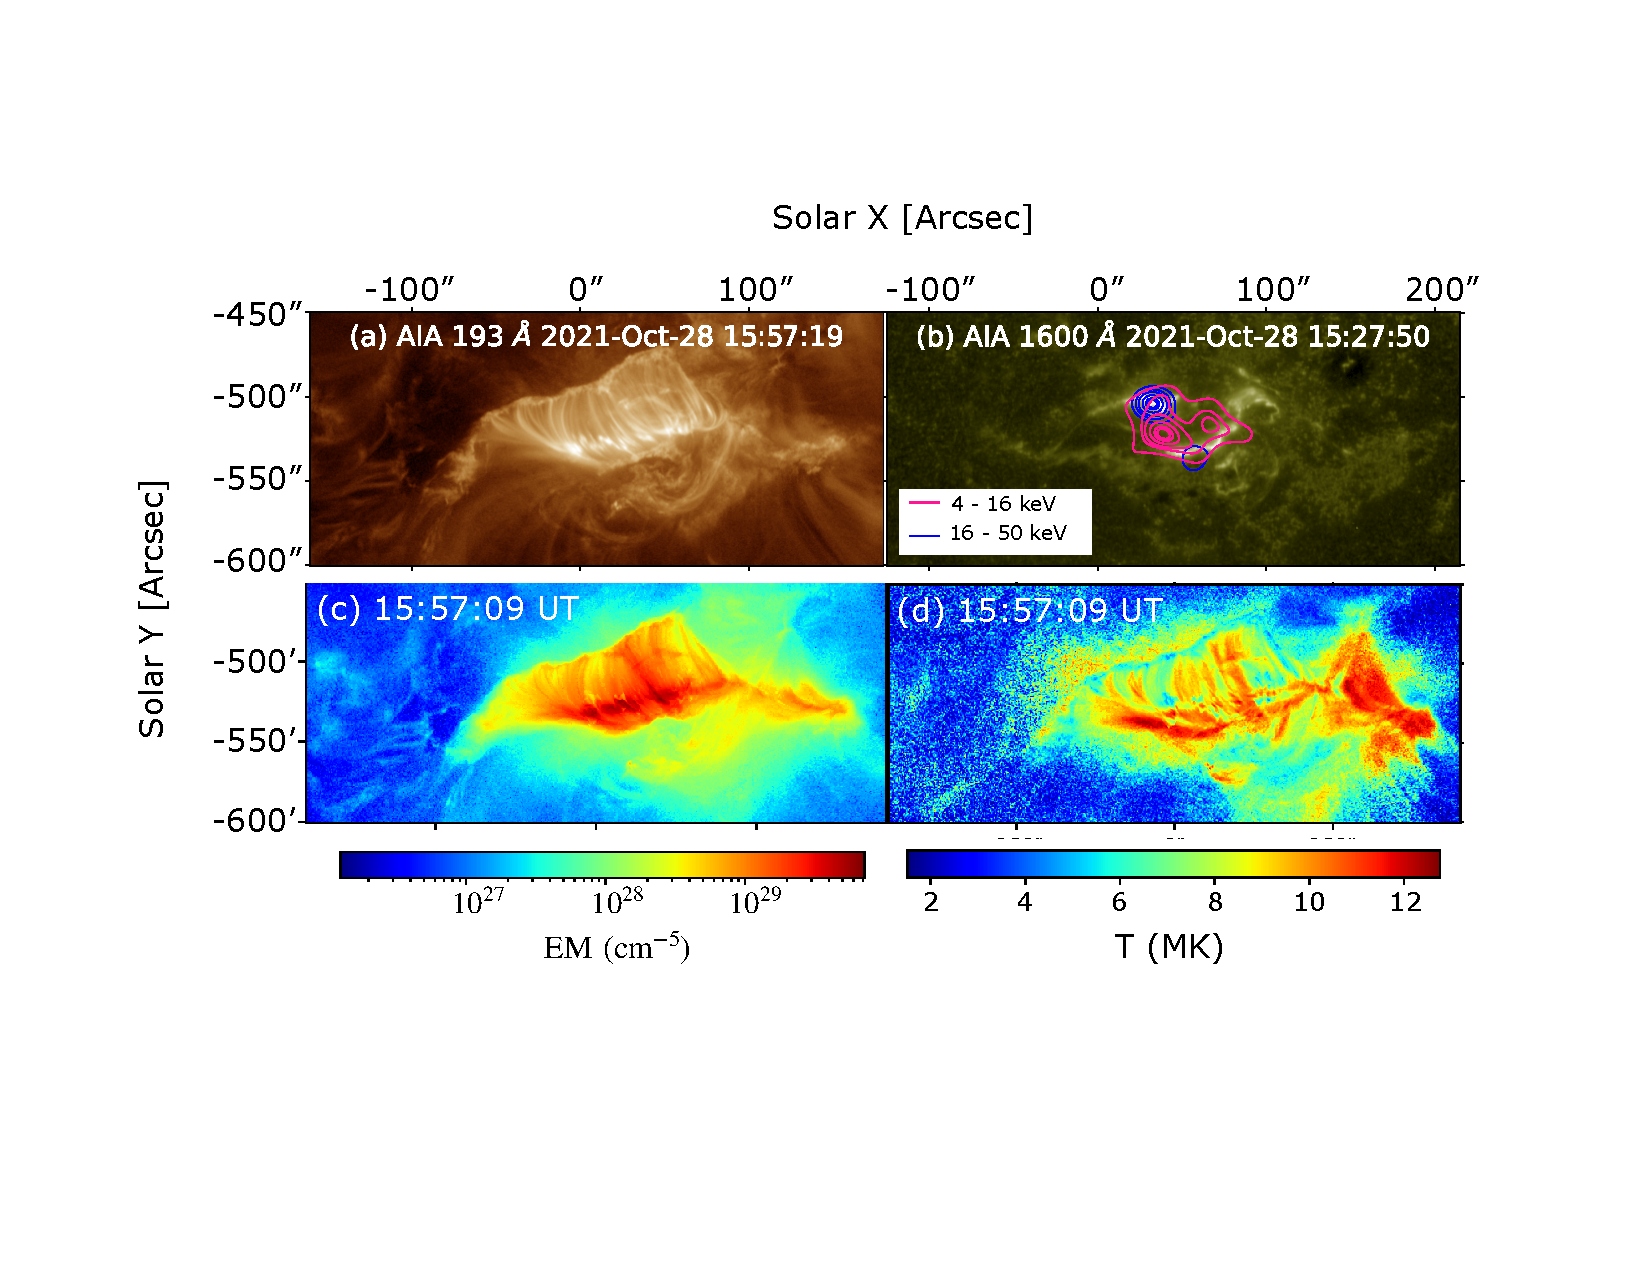
\includegraphics[width=0.9\textwidth,trim={2cm 5cm 3cm 3cm},clip]{oct28_align.pdf}
    \caption{Panel (a): the flare arcade in AIA 193 {\AA}. Panel (b): STIX soft X-ray contours (4 {--} 16 keV, solid pink lines) and hard X-ray contours (16 {--} 50 keV, solid blue lines) aligned to AIA 1600 {\AA} and over plotted. Panel (c): the emission measure map of the region for $5~<log(T)~<7.4$. Panel (d): the DEM weighted temperature map of the region.}
    \label{fig:flare}
\end{figure}
%%--------------------------

%%--------------------------
\begin{figure}[ht!]
\centering
    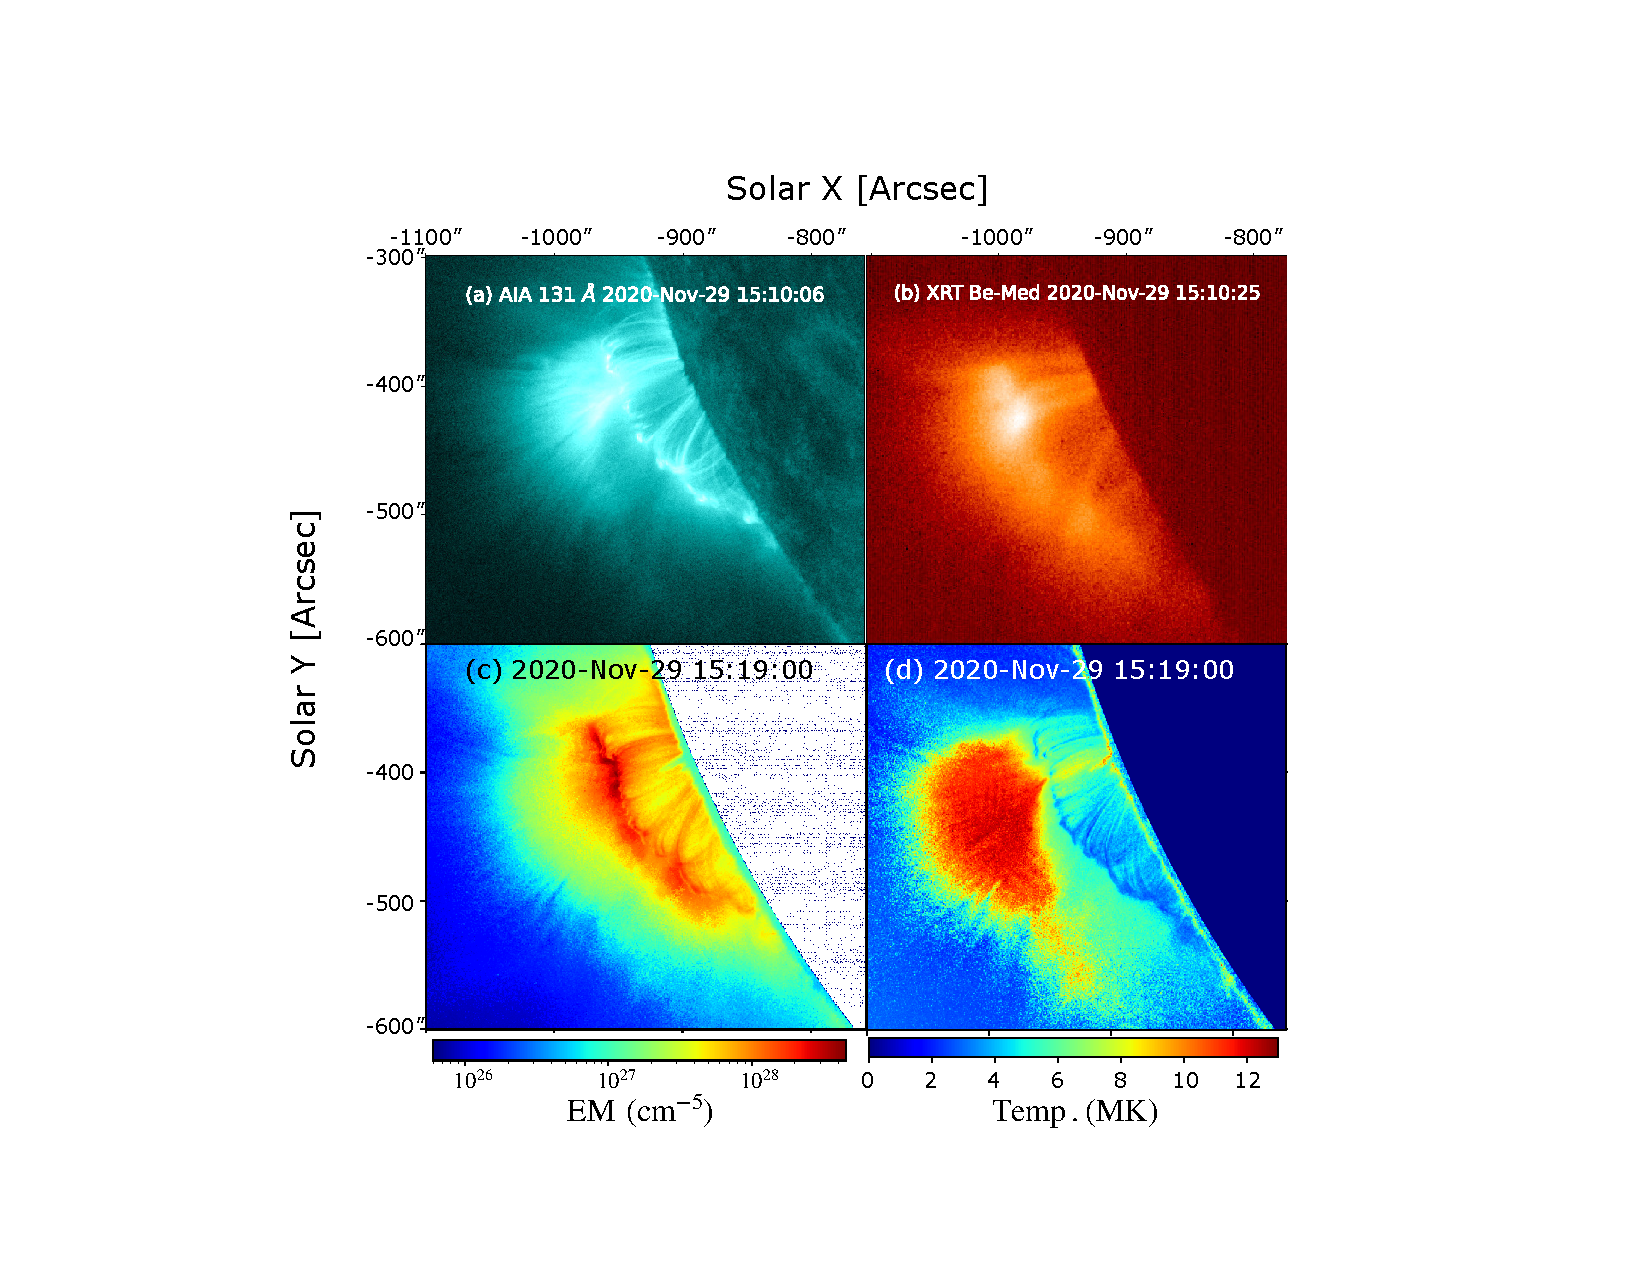
\includegraphics[trim={4.8cm 1.5cm 6cm 2.5cm},clip,width=0.9\textwidth]{nov_29_align.pdf}
    \caption{Panel (a): the flare arcade in AIA 131 {\AA}. Panel (b): {\it Hinode}/XRT Be-Med soft X-ray image recorded almost at the same time. Panel (c):  the DEM weighted temperature map of the region for $5~<log(T)~<7.4$. Panel (d): the emission measure map of the region for $5~<log(T)~<7.4$}
    \label{fig:flare2}
\end{figure}
%%--------------------------

%%%%%%%%%%%%%%%%%%%%%%%%%%%%%%%%%%%%%%%%
\subsubsection{Determining the LOS}\label{sec:los}
%%%%%%%%%%%%%%%%%%%%%%%%%%%%%%%%%%%%%%%%

To determine the line of sight (LOS) along individual pixels in the field of view (FOV), we initially estimate the height of the flare loop using observations from different vantage points. STEREO-A/EUVI observed both events from a different angle compared to AIA, resulting in geometric effects on the observations.

Fig.\ref{fig:flare_orient}a & b illustrates the geometric effect of observing from different vantage points. The magenta cross in Fig.\ref{fig:flare_orient}a represents a point at the top of the flare arcade. The LOS extends into the page through that point from the STEREO-A vantage. The red line in Fig.\ref{fig:flare_orient}b shows the LOS through the point in Fig.\ref{fig:flare_orient}a projected to the SDO/AIA point of view. Similar projections are shown in Fig.~\ref{fig:flare_orient2} for the Nov 29, 2020 flare.

To calculate the height of the flare loop, we utilize co-temporal STEREO-A 171 {\AA}, 195 {\AA}, and AIA 171 {\AA}, 193 {\AA} images with \textit{scc\_measure.pro}, available in the \textit{sswidl}. This routine enables us to select a point on the observation from one vantage point, and the LOS through the same point is shown on the observation from the other vantage point. By identifying similar emission characteristics, we can determine the 3D coordinates of the point (heliographic latitude, longitude, and radial distance). This measurement is repeated at various positions along the loop top to calculate the change in loop height across the arcade. However, it is important to note that the height estimation using \textit{scc\_measure.pro} is limited by our ability to identify ``similar emission characteristics'' between the AIA and STEREO-A observations.

%%--------------
\begin{figure}[ht!]
    \centering
    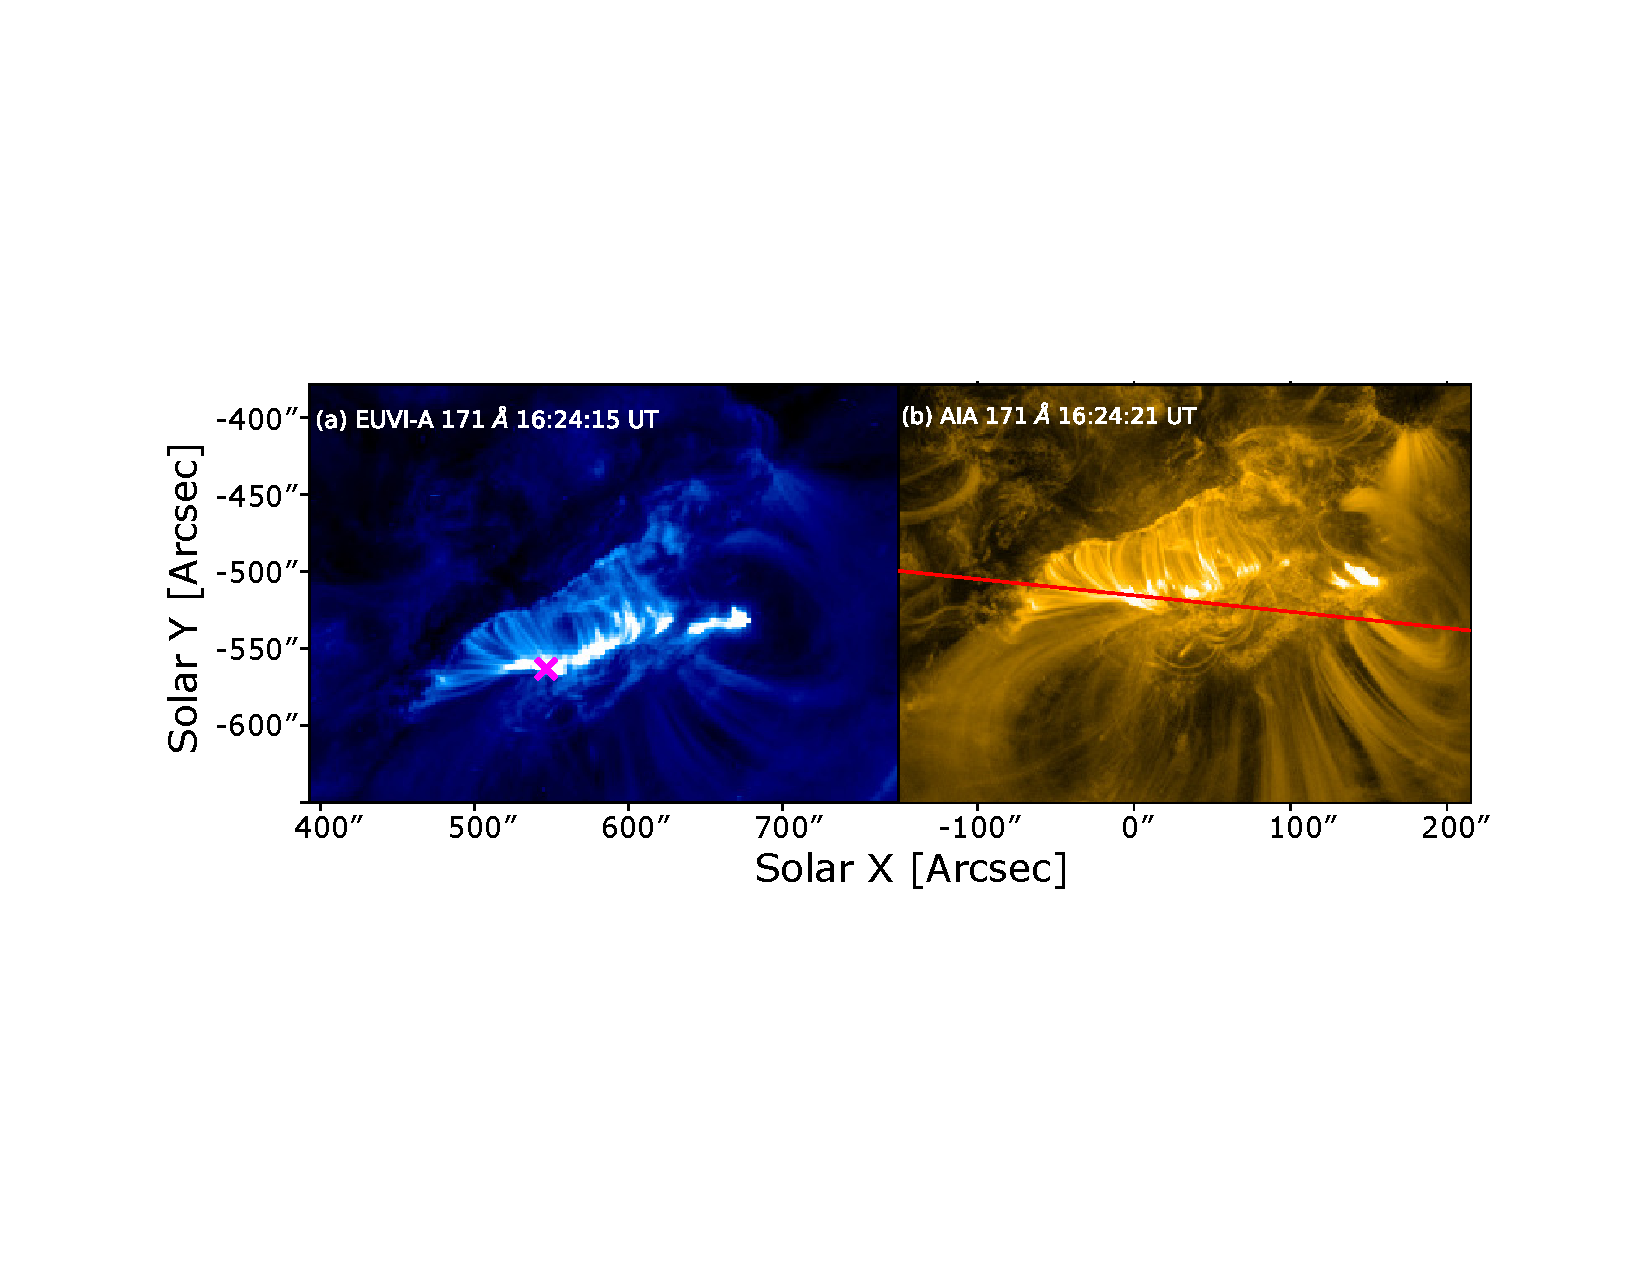
\includegraphics[width=\textwidth,trim={2cm 6cm 2cm 6cm},clip]{flare_orient.pdf}
    \caption{Panel (a): {\it STEREO-A}/EUVI 171 {\AA} observation of the flare arcade in the decay phase. The magenta cross marks a point on the top of the arcade. The LOS goes into the page through that point. Panel (b): SDO/AIA 171 {\AA} observation of the flare arcade. The red line marks the LOS through the arcade from the STEREO-A perspective projected to the AIA perspective.}
    \label{fig:flare_orient}
\end{figure}
%%--------------

%%--------------
\begin{figure}[ht!]
    \centering
    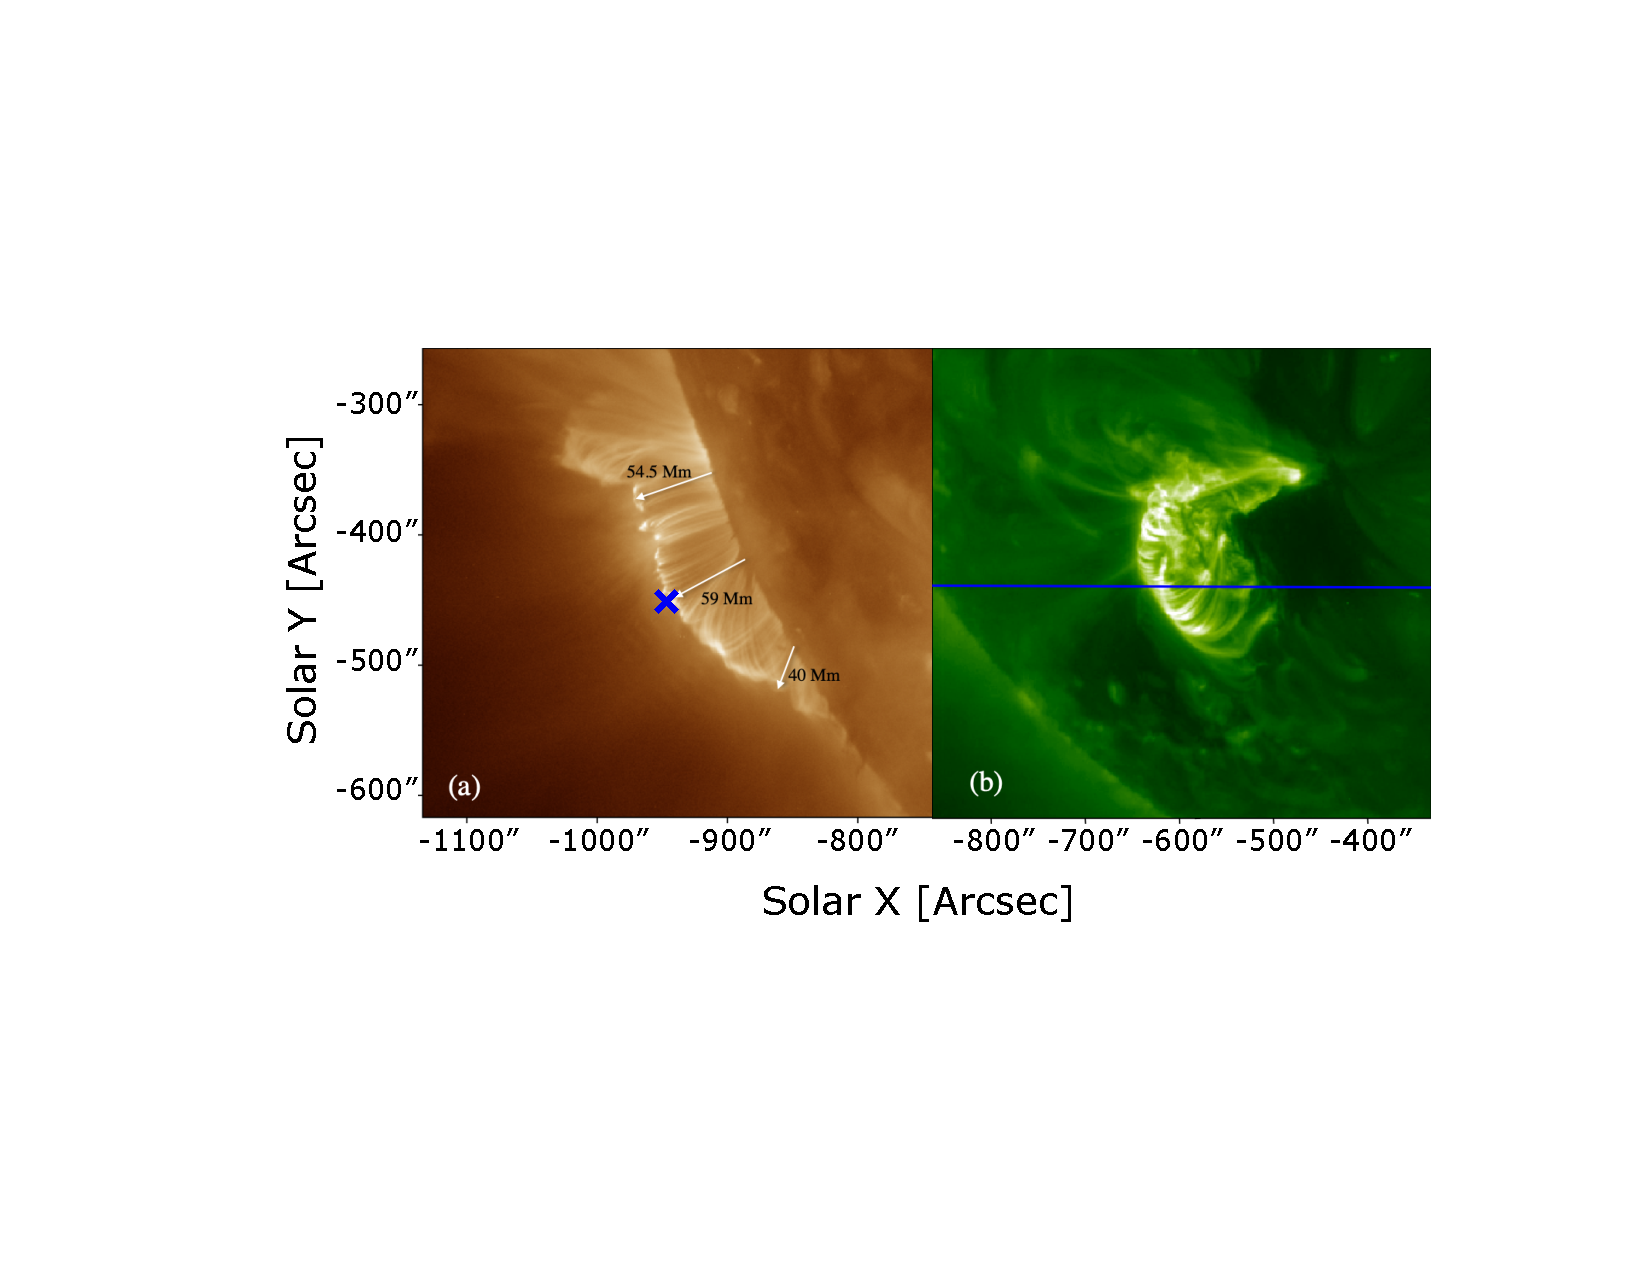
\includegraphics[width=0.9\textwidth,trim={4cm 5cm 3cm 5cm},clip]{nov29_triangulate.pdf}
    \caption{Panel (a): SDO/AIA 193 {\AA} observation of the Nov 29 flare in the decay phase. The blue cross marks a point on the top of the arcade. The LOS goes into the page from AIA perspective. Panel (b): {\it STEREO-A}/EUVI 195 {\AA} observation around same time. The blue solid line is the LOS from AIA perspective in panel (a) projected onto {\it STEREO-A} perspective. We can trace out the height of the flare arcade at various locations using \textit{scc\_measure.pro}. The height of the arcade at various points from the Sun's surface is marked in panel (a).}
    \label{fig:flare_orient2}
    \end{figure}
%%--------------

%%--------------
\begin{figure}[ht!]
    \centering
    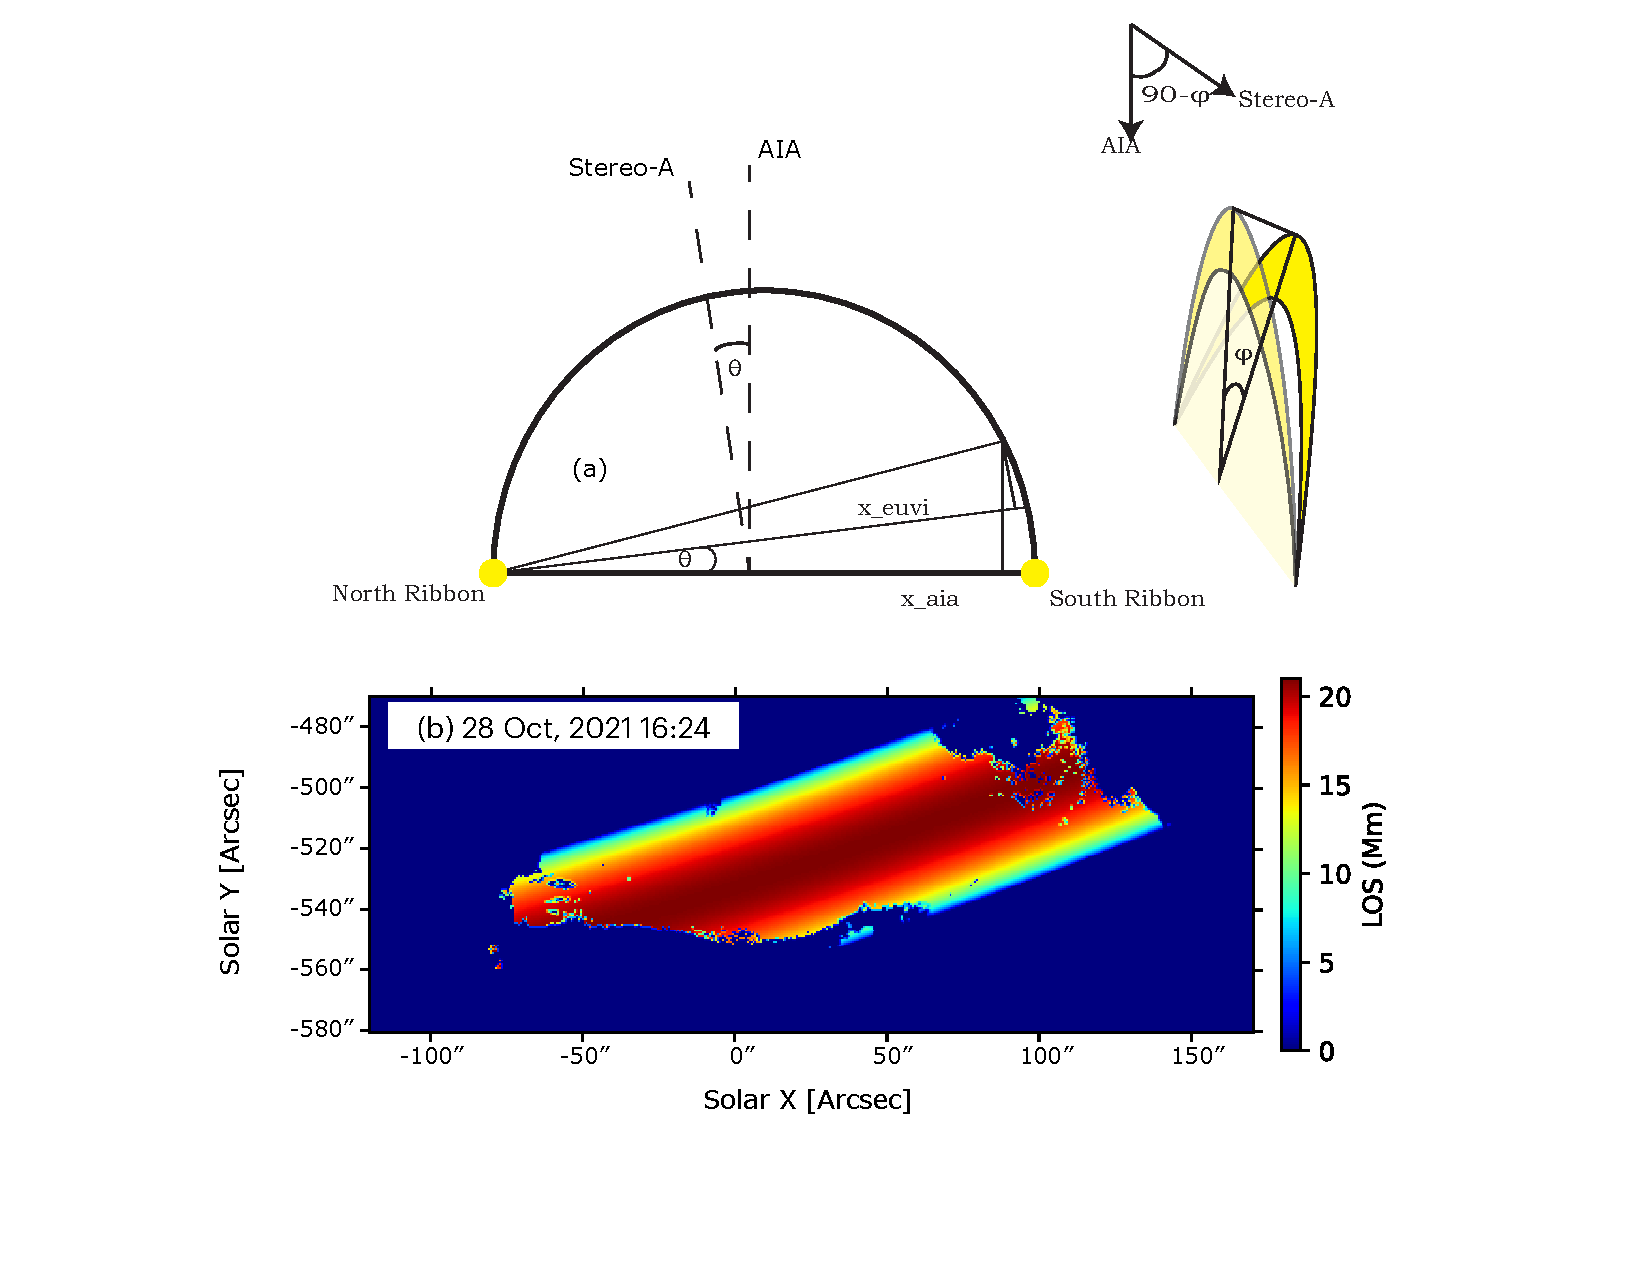
\includegraphics[width=0.8\textwidth,trim={3cm 2cm 3cm 0cm},clip]{flare_orient_pt2.pdf}
    \caption{Panel (a): Cartoon demonstrating the projection effects of a semicircular loop between STEREO-A and AIA vantages due to the difference between polar ($\theta$) and azimuthal ($\phi$) angles, respectively. Panel (b) : The calculated LOS map from the AIA perspective, with the estimated loop top height under the assumption of a semi-circular loop geometry.}
    \label{fig:flare_orient_2}
\end{figure}
%%--------------

To determine the extent of the flare arcade, we select pixels within an emission measure contour of 5\% of the peak emission measure value. This contour is calculated based on the emission measure inferred from the DEM, which reflects the density of plasma across the temperature range of $5<\log,(T)<7.4$. This approach provides a more comprehensive estimate of the flare arcade compared to methods based solely on intensity observations, which may miss significant portions of the arcade due to the highly multi-thermal nature of the plasma. Outside of the flare arcade, we assume a line of sight (LOS) thickness of approximately 2 Mm, corresponding to the average thickness of the chromosphere.

Fig. \ref{fig:flare_orient_2}b illustrates an example of the calculated LOS in the field of view (FOV) for the October 28, 2021 flare. The highest point of the flare arcade follows the ridge from southeast to northwest. An estimate of the highest point of the loop is approximately 22 Mm, consistent with previous estimates of the ridge height around 20 Mm from magnetic loop modeling \citep{longcope22}. Using the LOS map shown in the bottom panel of Fig. \ref{fig:flare_orient_2}, we calculate the thermal energy in every pixel of the flare using Equation \ref{eq:t_eneg}. This process is repeated for the flare loops in the November 29, 2020 event.

%%%%%%%%%%%%%%%%%%%%%%%%%%%%%%%%%%%%%%%%%%%%%%%%%%%%
\subsection{Energy in the non-thermal electrons}\label{sec:non-therm}
%%%%%%%%%%%%%%%%%%%%%%%%%%%%%%%%%%%%%%%%%%%%%%%%%%%%

To estimate the energy deposited by the non-thermal electrons in the X-class event on October 28, 2021, we analyze the STIX spectra. Figure \ref{fig:stix_an}.a illustrates the STIX light curve for different energy bands: 4 to 6 keV (solid black line), 6 to 12 keV (solid magenta line), 12 to 25 keV (solid yellow line), and 25 to 50 keV (solid blue line). The attenuator was activated around 15:28 UT to prevent saturation, notably reducing the intensity. The hard X-ray peak appears around 25 to 50 keV at approximately 15:28 UT, while the soft X-ray peak is discernible within the attenuated flux in the 6 to 12 keV band at approximately 15:30 UT.

Following the methodology outlined in \cite{emslie12}, we fit the STIX spectra at various time intervals during the flare's evolution using the `2vth' and `thick2' functions available in the OSPEX X-ray spectra fitting package within `{\it sswidl}'. A representative fit is depicted in Figure \ref{fig:stix_an} panel (b) for the time bin around 15:26-15:27 UT using the `2vth' (solid yellow) and `thick2' (solid green) functions. The `2vth' function represents a two-component thermal model, with parameters for emission measure, temperature of the thermal components, and relative abundances of various elements with respect to CHIANTI coronal abundances \citep{chianti1,chianti}. On the other hand, the `thick2' function assumes a non-thermal component attributed to bremsstrahlung from energetic electrons, described by a broken power-law injected spectrum $F_{0}(E_{0})~(e^{-}s^{-1}cm^{-2}keV^{-1})$ :

%%--------
\begin{equation}
    F_{0}(E_{0})=A
    \begin{cases}
        0, & E_{0}<E_{min} \\
        E_{0}^{-\delta_{1}}, & E_{min} \le E_{0} < E_{b} \\
        E_{0}^{-\delta_{2}}E_{b}^{\delta_{2}-\delta_{1}}, & E_{b} \le E_{0} < E_{max} \\
        0, & E_{max} \le E_{0}
    \end{cases}
\end{equation}
%%--------

In the fitting process, the model spectrum parameters, such as the normalization parameter \( A \), the low- and high-energy cutoffs \( E_{\text{min}} \) and \( E_{\text{max}} \), the break energy \( E_{\text{b}} \), and the power law indices \( \delta_{1} \) and \( \delta_{2} \) below and above the break, are constrained. We set the high-energy cutoff at \( 3.2 \times 10^{4} \) keV for all fits, as it is significantly higher than the energy range of interest (around \( 10^{1} \) keV), making its effect on the X-ray spectra negligible \citep{emslie12}.

The fitting procedure in `\textit{OSPEX}' is a forward fitting process. The parameters of the `\textit{2vth}' and `\textit{thick2}' functions are adjusted to generate a photon spectrum, which is then convolved through the detector response matrix to produce a count rate spectrum. This count rate spectrum is compared with the measured count rate spectrum, and an iterative process minimizes the \( \chi^{2} \) between them to refine the parameter estimates.

Table \ref{tab1} presents the fitted temperature of the hotter thermal component at various phases of the flare. These temperatures align with the temperature range (\( \log(T_{\text{max}}) = 7.4 \) and \( \log(T_{\text{min}}) = 5 \)) used to calculate the emission measure (EM) and differential emission measure (DEM) weighted temperature, as discussed in Section \ref{sec:therm}.

%%%%%%%%%%%
\begin{table*}[ht!]
    \centering
    \begin{tabular}{|cl||c|c|}
    \hline
         &  & log(T) & EM \\ 
         & \hspace{-1cm}Time (UT) & of hotter component & ($cm^{-3}$) \\
    \hline
        Impulsive phase & \hspace{1cm}15:26 & 7.098 & $10^{48}$\\
        HXR peak & $\sim$ 15:27:20 - 15:28:20 & 7.19 & $3\times 10^{48}$\\
        Right after SXR peak & $\sim$ 15:35:39 - 15:36:34 & 6.88 & $4.1\times 10^{49}$\\
        Into the decay phase & \hspace{0.9cm}14:48:20 & 6.5 & $2\times 10^{49}$\\
        \hline
    \end{tabular}
    \caption{Fitted temperature of the hotter component of the thermal plasma during various stages of the flare.}
    \label{tab1}
\end{table*}
%%%%%%%%%%%

The non-thermal energy in the electrons (\( U_{e} \)) at any instant \( t = t' \) can be estimated by integrating the best-fit electron energy spectrum:
\[
U_{e}(t=t') = \Delta t \int_{E_{\text{min}}}^{E_{\text{max}}} F_{0}(E_{0})(t=t') dE_{0}
\]
where the electron energy distribution is constrained by fitting the count spectra for the time interval \( t' - \Delta t/2 \leq t \leq t' + \Delta t/2 \).

The cumulative energy deposited into the footpoint over time by the non-thermal electrons is a good indicator of the source of the thermal energy of the plasma. We can estimate the cumulative energy deposited by the non-thermal electrons up until a certain instant \( t \) by summing the energy deposited at the footpoints from every time bin:
\[
U^{cumulative}_{e}(t) = \sum_{t'=t_{0}}^{t} U_{e}(t')
\]

%%--------------
\begin{figure}[ht!]
    \centering
    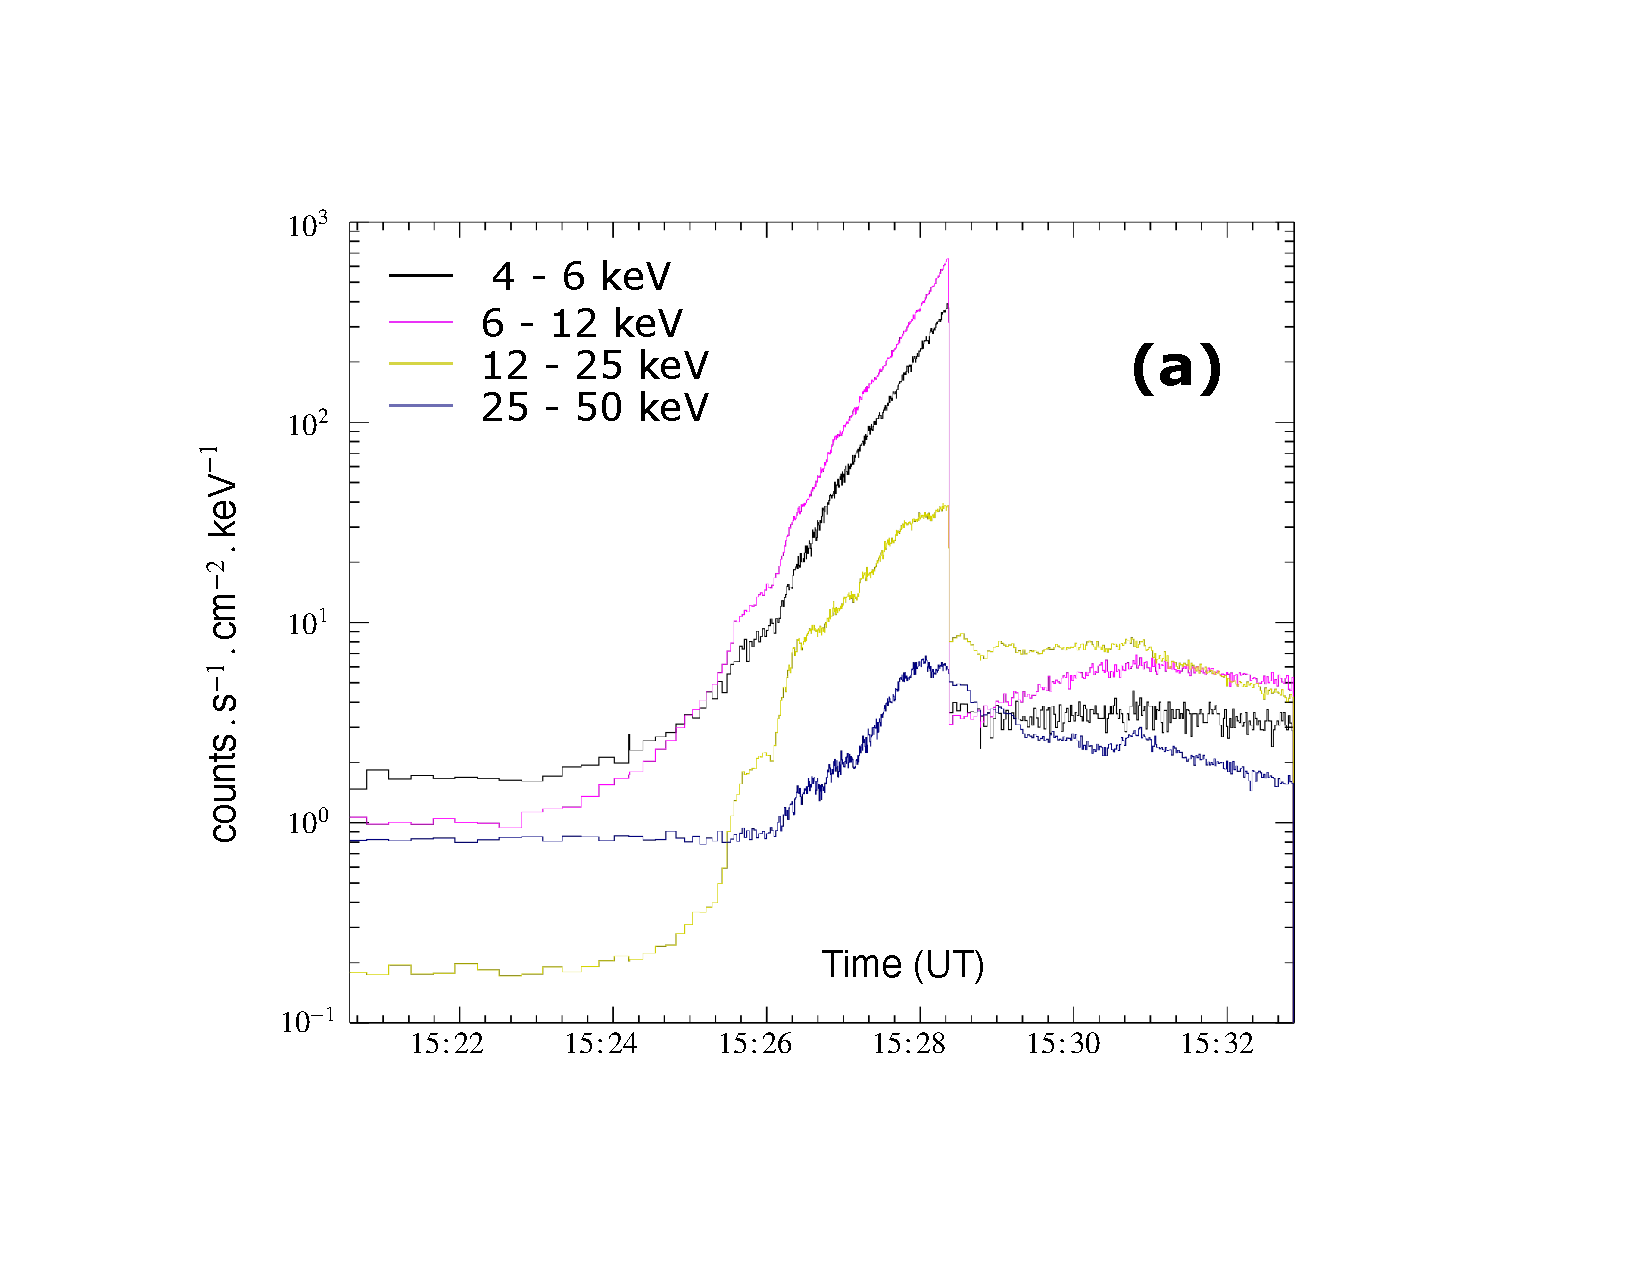
\includegraphics[trim={3cm 2cm 6cm 3.5cm},clip,width=0.54\textwidth]{oct28_lc_2.pdf} 
    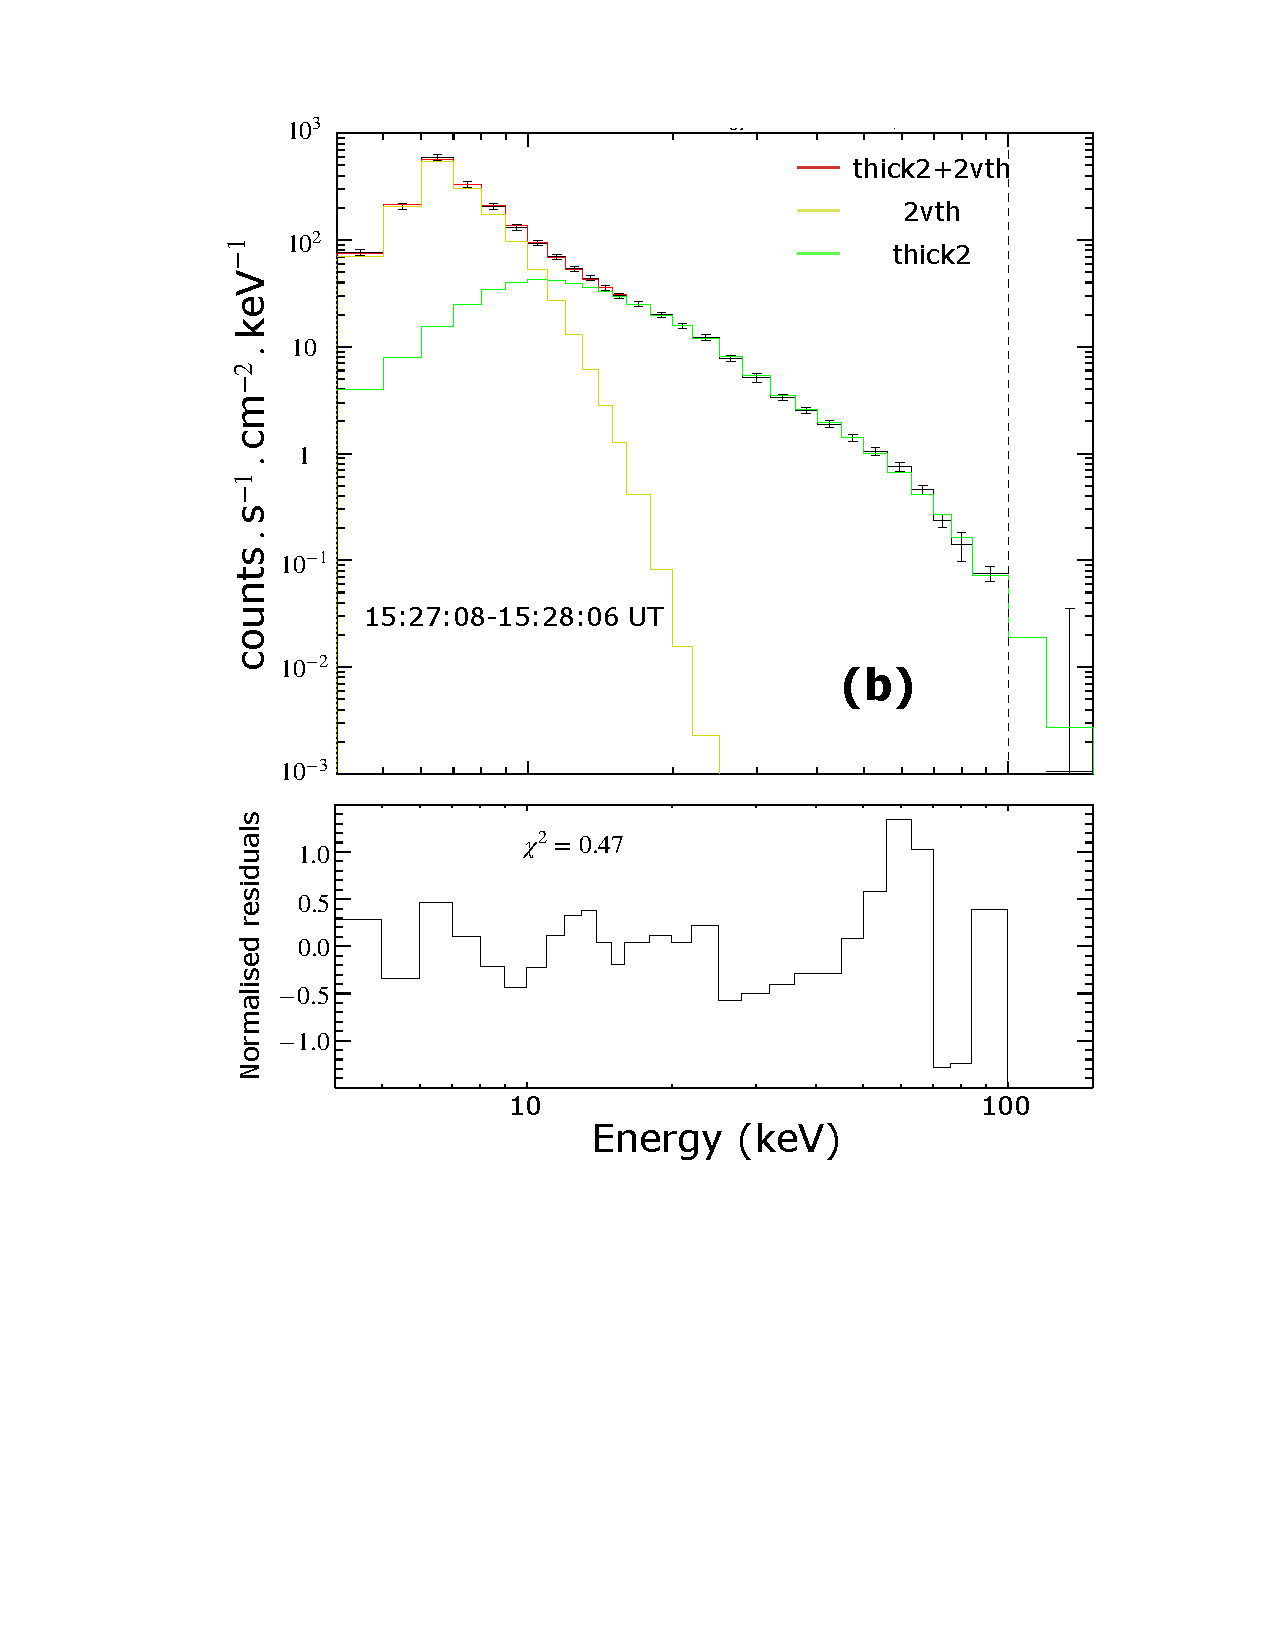
\includegraphics[trim={3.5cm 8cm 3cm 2cm},clip,width=0.45\textwidth]{oct28_fit_2.pdf}
    \caption{Panel (a): STIX light curve of the 2021 Oct 28 X-class event in different energy bands as labelled. The black, magenta, yellow and blue solid lines show the light curve in 4{--}6~keV, 6{--}12~keV, 12{--}25~keV and 25{--}50 keV. Panel (b): STIX spectra fit at 15:27{--}15:28 UT, during impulsive phase. We fit the spectra with `\textit{thick2}' (green solid line) and `\textit{2vth}' (yellow solid line). We show the complete fit function `\textit{2vth+thick2}' with the solid red line. The lower panel shows the normalized residuals of the fit.}
    \label{fig:stix_an}
    \end{figure}
%%--------------

%%%%%%%%%%%%%%%%%%%%%%%%%%%%%%%%%%%%%%%%%%%%%
\section{Results}\label{res}
%%%%%%%%%%%%%%%%%%%%%%%%%%%%%%%%%%%%%%%%%%%%%

%%###########%%
\begin{figure}[ht!]
    \centering
    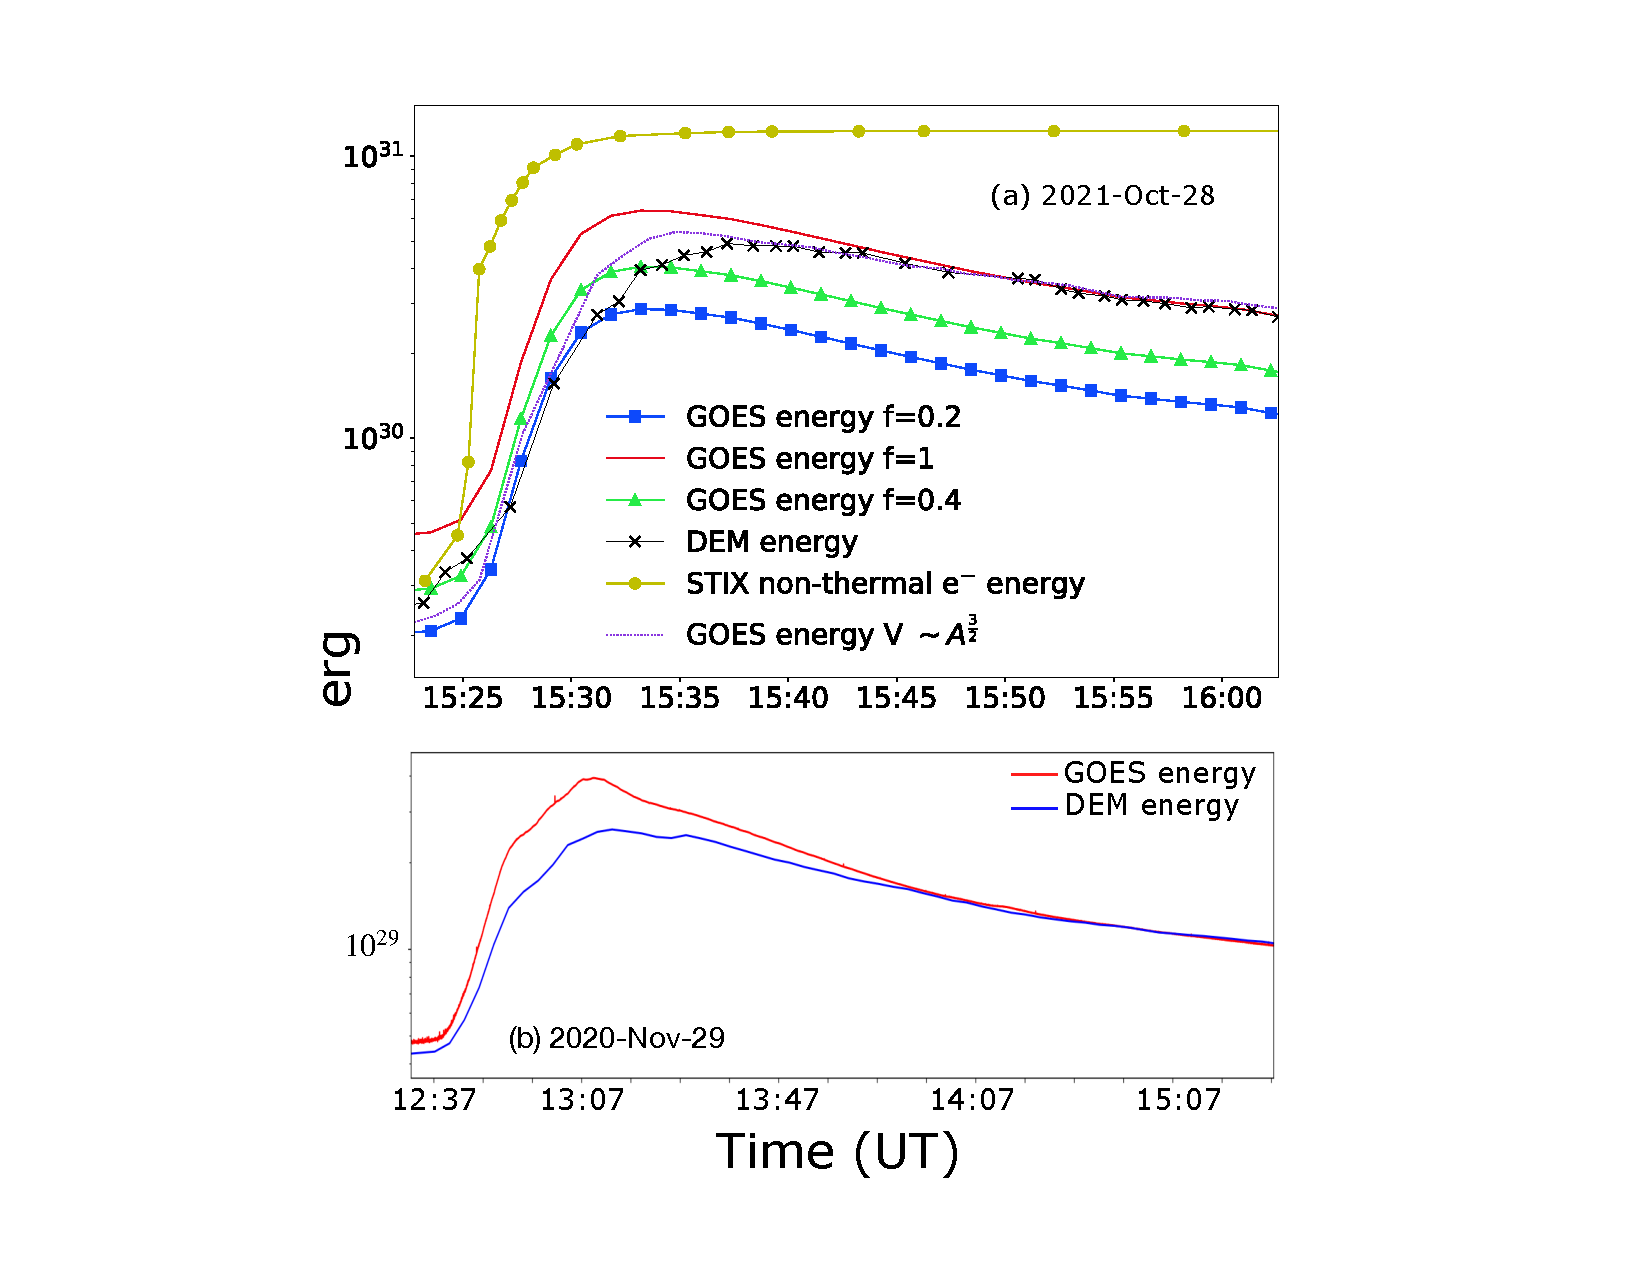
\includegraphics[trim={4cm 1cm 4cm 1cm},clip,width=0.8\textwidth]{flare_eneg.pdf}
    \caption{Panel (a): The calculated thermal energy as a function of time for the 2021 Oct 28 flare. The magenta dot-dashed line shows the thermal energy calculated from the GOES light-curve using the effective volume and a filling factor \textit{f}~=~1. The red dot-dashed line and the black dashed line shows the energy calculated from the GOES light-curve and the effective volume with filling factor \textit{f}~=~0.4 and \textit{f}~=~0.2, respectively. The blue solid line shows the thermal energy estimated using the DEMs calculated from the AIA obeservations. The black solid line shows the thermal energy calculated from the GOES light curve, but the volume inferred from the area of the of the flaring arcade with STIX SXR images, under the assumption that $V\sim A^{\frac{3}{2}}$. Panel (b): The calculated thermal energy as a function of time for the 2020 Nov 29 flare. The red line shows the thermal energy calculated from the GOES light curves, using a constant effective volume. The blue curve shows the thermal energy calculated from the DEMs inferred from the imaging and a varying volume from the imaging.}
    \label{fig:eneg}
\end{figure}
%%###########%%

%%###########%%
\begin{figure}[ht!]
    \centering
    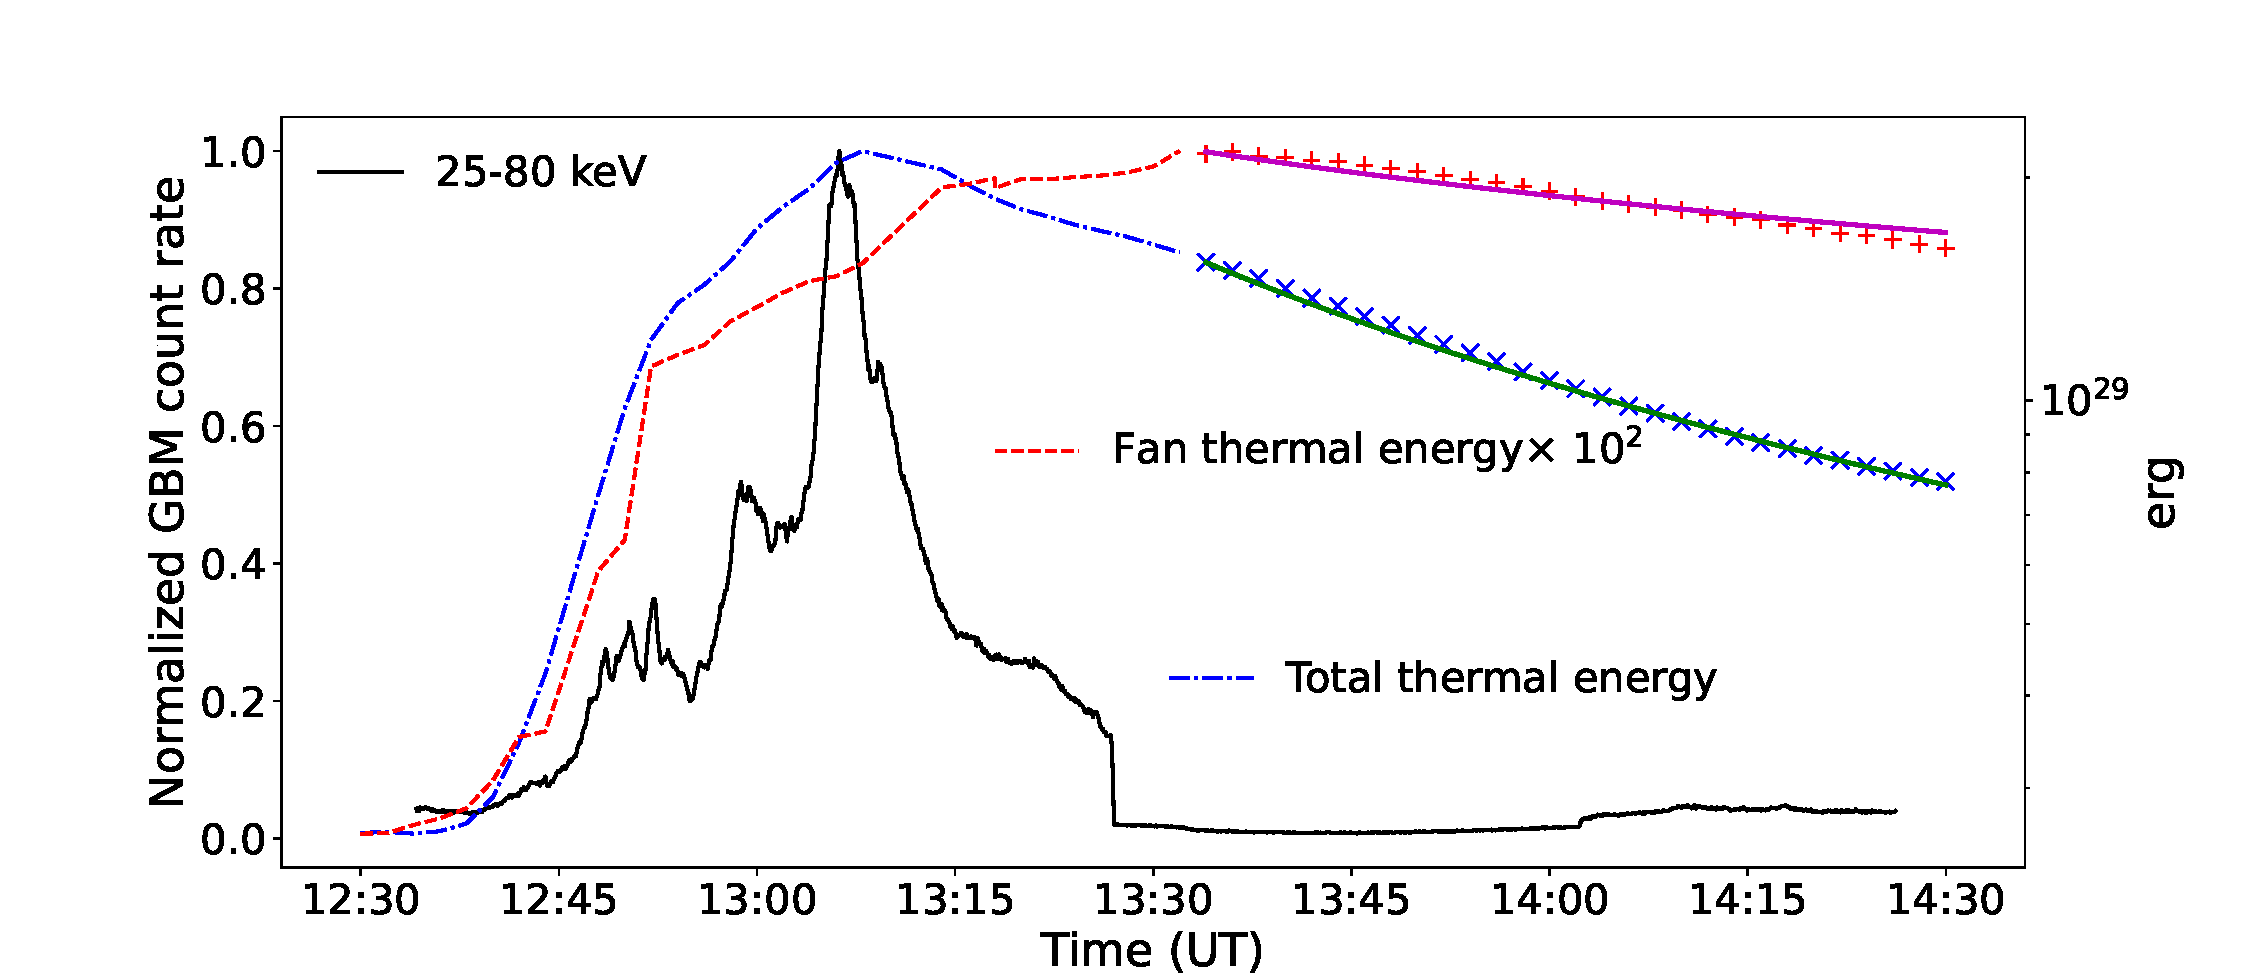
\includegraphics[trim={2cm 0cm 1cm 0cm},clip,width=0.8\textwidth]{fan_eneg.pdf}
    \caption{Calculated thermal energy for the 2020 Nov 29 flare. Total thermal energy of the flare (blue dot-dashed) in comparison to the thermal energy from the fan (red dashed). The magenta and the green solid line show the fit to the thermal energy output to the fan and the loop's thermal output. Fermi hard X-ray count (black) peaks around the same time as the total thermal output.}
    \label{fig:fan_eneg}
    \end{figure}
%%###########%% 

Figure~\ref{fig:eneg}.a shows the thermal and non-thermal energy calculated for the 2021 October 28 event. The black solid curve with crosses shows the thermal energy calculated from the DEMs. The red solid curve shows the thermal energy calculated from the {\it GOES} light curve and the effective volume calculated assuming an RTV loop \citep{rtv78,serio91}. We use the {\it GOES} emission measure, temperature with a volume filling factor \textit{f}~=~1, to estimate an effective loop length for the flare and from that, calculate an effective volume. Note that the implicit assumption of mechanical equilibrium only holds during the decay phase of the flare. So, the effective volume estimated here would only be appropriate in the decay phase. The green solid curve with triangles and the blue solid curve with squares show the same {\it GOES} thermal energy, with volume filling factor \textit{f}~=~0.4 and \textit{f}~=~0.2, respectively. The blue dashed curve shows the thermal energy calculated from the {\it GOES} light curve, but the volume inferred from the area of the flaring region from the STIX soft X-ray contours, under the assumption that $V\sim A^{\frac{3}{2}}$.

The lime green solid line with circles in Fig.~\ref{fig:eneg}.a, shows the cumulative energy in the non-thermal electrons. This quantity is the amount of energy deposited at the flare foot points, and one of the sources of the thermal energy of the flare. The cumulative non-thermal energy of electrons $\simeq~1.2\times 10^{31}$ erg $>$ peak thermal energy calculated from the DEM estimates $\simeq~5\times 10^{30}$ erg. This is usual for an X-class flare. The differences in the estimates of thermal energy, due to different estimations of volume, also affects the partition between the thermal and non-thermal energies of flares. The efficiency of converting the energy deposited by non-thermal electrons into the thermal energy of the ambient plasma results in this partition and as a result, the volume estimation is a key parameter in understanding the conversion of non-thermal energy into thermal energy in flares.

The interesting trend in Fig.~\ref{fig:eneg}.a is that the thermal energy calculated from the constrained DEMs (solid black curve with crosses) is closer to a volume filling factor \textit{f}~=~0.2 in the impulsive phase, but is asymptotic with a filling factor \textit{f}~=~1 (solid red curve) during the decay phase. This indicates that the flare loops during the impulsive phase do not fill up apparent volumes similar to those in the decay phase. The change in the effective filling factor is indicative of the sharp change in the volume during the impulsive phase.

For the 2020 November 29 event, the {\it STEREO-A} perspective looks down into the supra-arcade plasma sheet. Thus the LOS of this feature can not be calculated as demonstrated in Section \ref{sec:los} for the supra-arcade pixels. For the supra-arcade fan pixels in the FOV, we assume a LOS $\simeq~8~\textrm{Mm}$, as suggested in several other studies \citep[see e.g.,][]{savage10,seaton17,li18}. We use these calculated LOS maps, along with equation~\ref{eq:t_eneg_1} to estimate the thermal energy as a function of time.

Figure \ref{fig:eneg}.b shows the energy calculated for the November 29th event. The blue solid curve shows the thermal energy calculated from the DEMs. The red solid curve shows the thermal energy calculated from the GOES light curves and the constant effective volume calculated assuming an RTV loop with a volume filling factor \textit{f}~=~1. The thermal energy shows similar characteristics as the October 28th, 2021 event. The RTV loop effective volume clearly is an overestimation in the rise phase of the the flare, and agrees very well in the decay phase.

There have been several studies that suggest that the plasma in the fan is directly heated \citep{hanneman14,chen17,reeves17,warren18,cai22,xie23}. Unlike the flare arcade, the thermal output of the fan is not directly related to the energy deposited by the non-thermal electrons and ions at the foot point. Hence, this different mechanism should also be reflected in the time evolution of the thermal output of the fan, compared to the thermal output of the loops. Under the assumption of the LOS~$\mathrm{\sim 8~Mm}$ in the fan region, we separately calculate the contribution from the fan to the total thermal energy for the 2020 Nov 29 event.

Figure~\ref{fig:fan_eneg} shows the thermal energy of the fan as a function of time (red dashed line) in comparison to the total thermal energy of the 2020 Nov 29 event (blue dot-dashed line). The thermal energy form the fan is $\sim$ two orders of magnitude lower than the total thermal energy of the event. The thermal energy of the fan also peaks much later ($\sim$ 20 minutes) compared to the total thermal energy. After the thermal energy of the fan peaks, the thermal energy of the fan (red + sign) and the total thermal energy of the event (blue crosses) are fitted with a power law of the form $at^{-\delta}$ as a function of time. The fits are shown with magenta and green solid line for the fan and the total thermal energy, respectively. The value of the power law index are -0.95 and -1.1, respectively, for the fan and the total thermal output. The plots shows that the thermal energy of the fan decay slower compared to the total thermal output. The normalized {\it Fermi} GBM 25 {--} 80 keV count rate (black solid line) peaks at a similar time as the total thermal energy of the event.

%%%%%%%%%%%%%%%%%%%%%%%%%%%%%%%%%%%%%%%%%%%%%
\section{Outlook}\label{sec:out}
%%%%%%%%%%%%%%%%%%%%%%%%%%%%%%%%%%%%%%%%%%%%% 


We have used AIA, SUVI, and XRT observations to calculate DEM maps and estimate the thermal energy for two solar flares as a function of time. We have used observations from AIA and {\it STEREO-A} to calculate the geometry of the flare loops and estimate the LOS for the AIA observations. We have shown that the accurate estimation of volume can have significant implications for thermal energy estimates. For the 2020 November 20 flare, we have also estimated the thermal energy for the fan and compared the evolution of the thermal energy of the fan with respect to the total thermal energy of the event. We have shown that the thermal energy of the fan decays slower compared to the total thermal energy of the event. This result suggests that a fundamentally different heating mechanism is responsible for the thermal output of the fan.

The thermal energy of the flares is given as, $U_{Th}\simeq 3n_{e}k_{B}TVf$. The electron number density is given by, $n_{e}~=~\sqrt{\sfrac{EM^{v}}{Vf}}~\implies~U_{Th}~=~3k_{B}T\sqrt{EM^{v}\times~Vf}$, where $EM^{v}$ is the volume emission measure (in units of $cm^{-3}$). A filling factor, \textit{f} $<$ 1 decreases the thermal energy by $\sim f^{\sfrac{1}{2}}$. There are very diverse results reported on \textit{f}. X-ray observations have generally constrained within $0.1<\textit{f}<1$\citep{jak11,guo12}, while it is usually constrained to much lower values $0.001<\textit{f}<0.1$ in EUV\citep{ash&ash08}. The filling factor can also be constrained by imposing the requirement that the flare plasma has to be contained via magnetic pressure. From this constraint it can be inferred that the required coronal magnetic field strength $B_{cor}$ $\sim f^{-\sfrac{1}{4}}$\citep{caspi14,warmuth16a,warmuth16b}. These studies rule out values of $\textit{f}<0.1$. Similar results were obtained from spectroscopic observations of density sensitive \ion{Fe}{11} lines \citep{miligan12}.

It is easy to infer from our findings that a single value of volume filling factor is inadequate to describe the evolution of thermal energy throughout the duration of the flare. We need to estimate the volume as a function of time rather than depending on a filling factor. In Fig.~\ref{fig:eneg}.a, the thermal energy calculated from {\it GOES} with various filling factors demonstrates this concept perfectly. During the impulsive phase, the thermal energy calculated from the DEMs is consistent with \textit{f}=0.2, and later in the decay phase, it is consistent with \textit{f}=1. This result demonstrates how the volume of the flare arcade is changing over time with respect to the volume in the decay phase. The thermal energy calculated from $V\sim A^{\frac{3}{2}}$ assumption agrees well with the thermal energy calculated from constrained DEMs in the decay phase. But it still predicts higher energy in the impulsive phase. This discrepancy might signify that the assumption of self-similar expansion might not be valid at the initial sharp rise in the impulsive phase for some flares.

Our results are in line with the findings of \cite{hilarie05}. They demonstrated from {\it RHESSI} imaging for a sample of 9 M and C class flares that the volume estimation with the assumption of self-similar expansion resulted in thermal energy higher than the non-thermal energy during the impulsive phase (For more details, refer to \cite{hilarie05} Table 5 and the corresponding discussion). A statistically inferred representative filling factor might serve perfectly well for estimating the energies near the thermal peak for a sample of flares. Since we are trying to quantify the evolution of the energy over time for individual flares, we require more accurate estimates of the volume.

Our results also demonstrate the utility of estimating the volume from different vantages as a function of time. For events like the X-class event on 2021 October 28, the on-disk imaging allows the estimation of the volume from the flare ribbon area under the assumption of self-similar expansion. But for scenarios like the limb event 2020 November 29, where the flare ribbons are not visible from any imaging observation, or the visible foot point and/or visible portions of the loop are projected at a very high angle, estimating the volume of the loop by calculating the height of the loop at various points serves as an important tool in estimating the thermal energy at various phases of the flare.

In Figure~\ref{fig:fan_eneg}, the thermal energy from the fan (red dashed line ) is $\sim$ two orders of magnitude lower than the total thermal energy of the event (blue dot-dashed line). The thermal energy also peaks much later ($\sim$ 20 minutes) compared to the total thermal energy. This result shows that the fan plasma is being heated directly by a process different from the flare arcade (e.g. SADs \citep{reeves17}, plasma flow turbulence \citep{xie23}). The fan also cools slower than the arcade, which indicates that either continuous heating is present in the fan during the decay phase of the flare or there is suppression of cooling \citep[e.g.][]{xie23}. The event had both foot points occulted from the Earth's perspective, so it is a fair assumption that most of the hard X-ray is from the loop top coronal source. This circumstance explains the near-simultaneous peak in {\it Fermi} hard X-ray (black solid line) and the thermal energy peak from the flare.

Our results exhibit the importance of different solar missions that can observe the Sun with higher spatial resolution (to resolve the finer structures better) and from various vantages (to triangulate the geometry). The ability to spatially resolve the temperature structure of the flaring plasma not only gives us a better estimation of the thermal energy, but it also allows us to spatially separate various portions of the flaring plasma (e.g. for the 2020 November 29 event, we could separate the contribution of the fan from the total thermal energy). This separation enabled us to demonstrate that a different heating mechanism was at play in the fan. However, we do note that the reliability of any such estimations needs to be rigorously tested with observations of various flares from various geometric projections.



\clearpage
%
\chapter{Estimating thermal energy of two Solar Flares}\label{c:chap7}
\chaptermark{Solar flare energy}
\begin{quote}
{\em ~~~~~~~This thesis chapter originally appeared in the literature as} \\
{authors,
{\em journal reference info}}
\end{quote}
\justifying

%%----------------------------------------------------
\section{Introduction} \label{sec:intro}
%%----------------------------------------------------

The Solar Ultraviolet Imaging Telescope onboard {\it Aditya-L1} \citep[{\it Aditya-L1}/SUIT,][]{article,ghosh16,adityal1,suit_main} provides a targeted probe into the Chromosphere and Transition region. It provides continuous full-disk and Region of Interest (RoI) coverage of the Sun in eleven pass bands. The details of these bands are provided in chapter~\ref{c:chap3} Tab.~\ref{tab:science_filters}. The eight narrow bands provide coverage across the \ion{Mg}{2} k and h lines, \ion{Ca}{2} h line, the CN band, red and blue wing of the \ion{Mg}{2} window and parts of the NUV continuum. As alluded earlier, this provides unprecedented coverage of the Chromospheric and Transition region structure of solar flares.

The {\it Aditya-L1} was launched on September 2nd, 2023. The first light observations were made on December 5th, 2023 while the payload was still in cruise phase. For the majority of the cruise phase the payload only operated in the 2k synoptic mode, i.e. it only captured continuous (2k $\times$ 2k) observations in NB4 (\ion{Mg}{2} h line) with one minute cadence. The L1 insertion was carried out on January 6th, 2024. Following that the payload also started taking (4k $\times$ 4k) observations in all eleven science filters. Various components of the flare detection algorithm were progressively turned on. In this chapter we discuss some of the initial flare observations made by SUIT. The first flare triggered by the flare detection algorithm was a X6.3 flare from north-west corner of the disk on February 22nd, 2024, which was also observed by several other instruments {\it e.g.} {\it SDO}/AIA, {\it IRIS}, {\it SO}/STIX. During the cruise phase, SUIT also observed a X1 flare from the south-east limb of the Sun on December 31st, 2023. We only have observations in the NB4 (\ion{Mg}{2} h line) channel for this flare. But this provides us with an unprecedented view of post-flare loops and possibly reconnection slingshot in the \ion{Mg}{2} line. Subsequent portions of this chapter will be divided into two parts, where we discuss the observations of these two flares separately.

%%----------------------------------------------------
\section{X6.3 flare observed on Feb 22nd, 2024} \label{sec:feb_22nd}
%%----------------------------------------------------

NOAA AR 13590 was visible on the north-east of the Solar disk on February 22, 2024. The AR was around a large sunspot in a cluster of sunspots, accompanied by a complex magnetic field structure. The active region flared multiple times during the same day, including an X1.7 flare that peaked around $\sim$ 06:32 UT, an M4.8 flare that peaked around $\sim$ 20:46 UT and an X6.3 flare that peaked $\sim$ 22:34 UT . \suit~is equipped with an onboard flare detection algorithm. Once the flare detection algorithm flags a flare and localizes the position of the flare on the detector, the program sequence prioritizes reading a fixed smaller Region of Interest (RoI) around the location for fast, higher cadence observation (for further details, please refer to \cite{flare_det}). The X6.3 flare was one of the first flares to be localized by the on-board flare detection algorithm. \suit~did not observe the X1.7 flare because, during that time, the payload was off-pointed to verify the stellar calibration program sequences. The flares were also observed by {\it SDO}/AIA, {\it SO}/STIX. {\it IRIS} observed the eastern edge of the X6.3 flare ribbons in a small [66\arcsec,62\arcsec] field of view (FoV) with a 4 step raster and 15 s raster cadence.

We show the light curve arising from the whole RoI observation in comparison to {\it GOES} flux in Fig.~\ref{fig:flare_full}. In Fig.~\ref{fig:flare_full}.b, we plot the AIA 1600 {\AA} (dashed blue line) and AIA 1700 {\AA} (black dot-dashed line), in comparison to the {\it GOES} 1 {--} 8 {\AA} light curve (Solid red line) for both the flares. In Fig.~\ref{fig:flare_full}.b, we show the GOES 1 {--} 8 {\AA} light curve in comparison to the NB3 (\ion{Mg}{2} k 279.6 nm, black dotted), NB4 (\ion{Mg}{2} h 280.3 nm, green dot-dashed) and NB8 (\ion{Ca}{2} h 396.85 nm, magenta dashed) light curves. NB4 light curve is offset from NB3 by -0.1 for better visibility. The NB8 light curve exhibits lower contrast and does not show a sharp peak compared to NB3 and NB4. The other interesting trend is exhibited by the continuum channels NB5, NB6 and NB7 in Fig.~\ref{fig:flare_full}.c, as a conspicuous rise in the continuum intensity is seen after both flares. In Fig.~\ref{fig:flare_full}.d we plot the {\it GOES} 1 {--} 8 {\AA} light curve in comparison to the STIX hard (25 {--} 50 keV, black dashed) and soft (5 {--} 10 keV, green dotted) X-ray light curve. The hard X-ray observation from STIX peaks at a time similar to that of NB3, NB4, and NB8.

%%%%%%%%%
\begin{figure}[ht!]
    \centering
    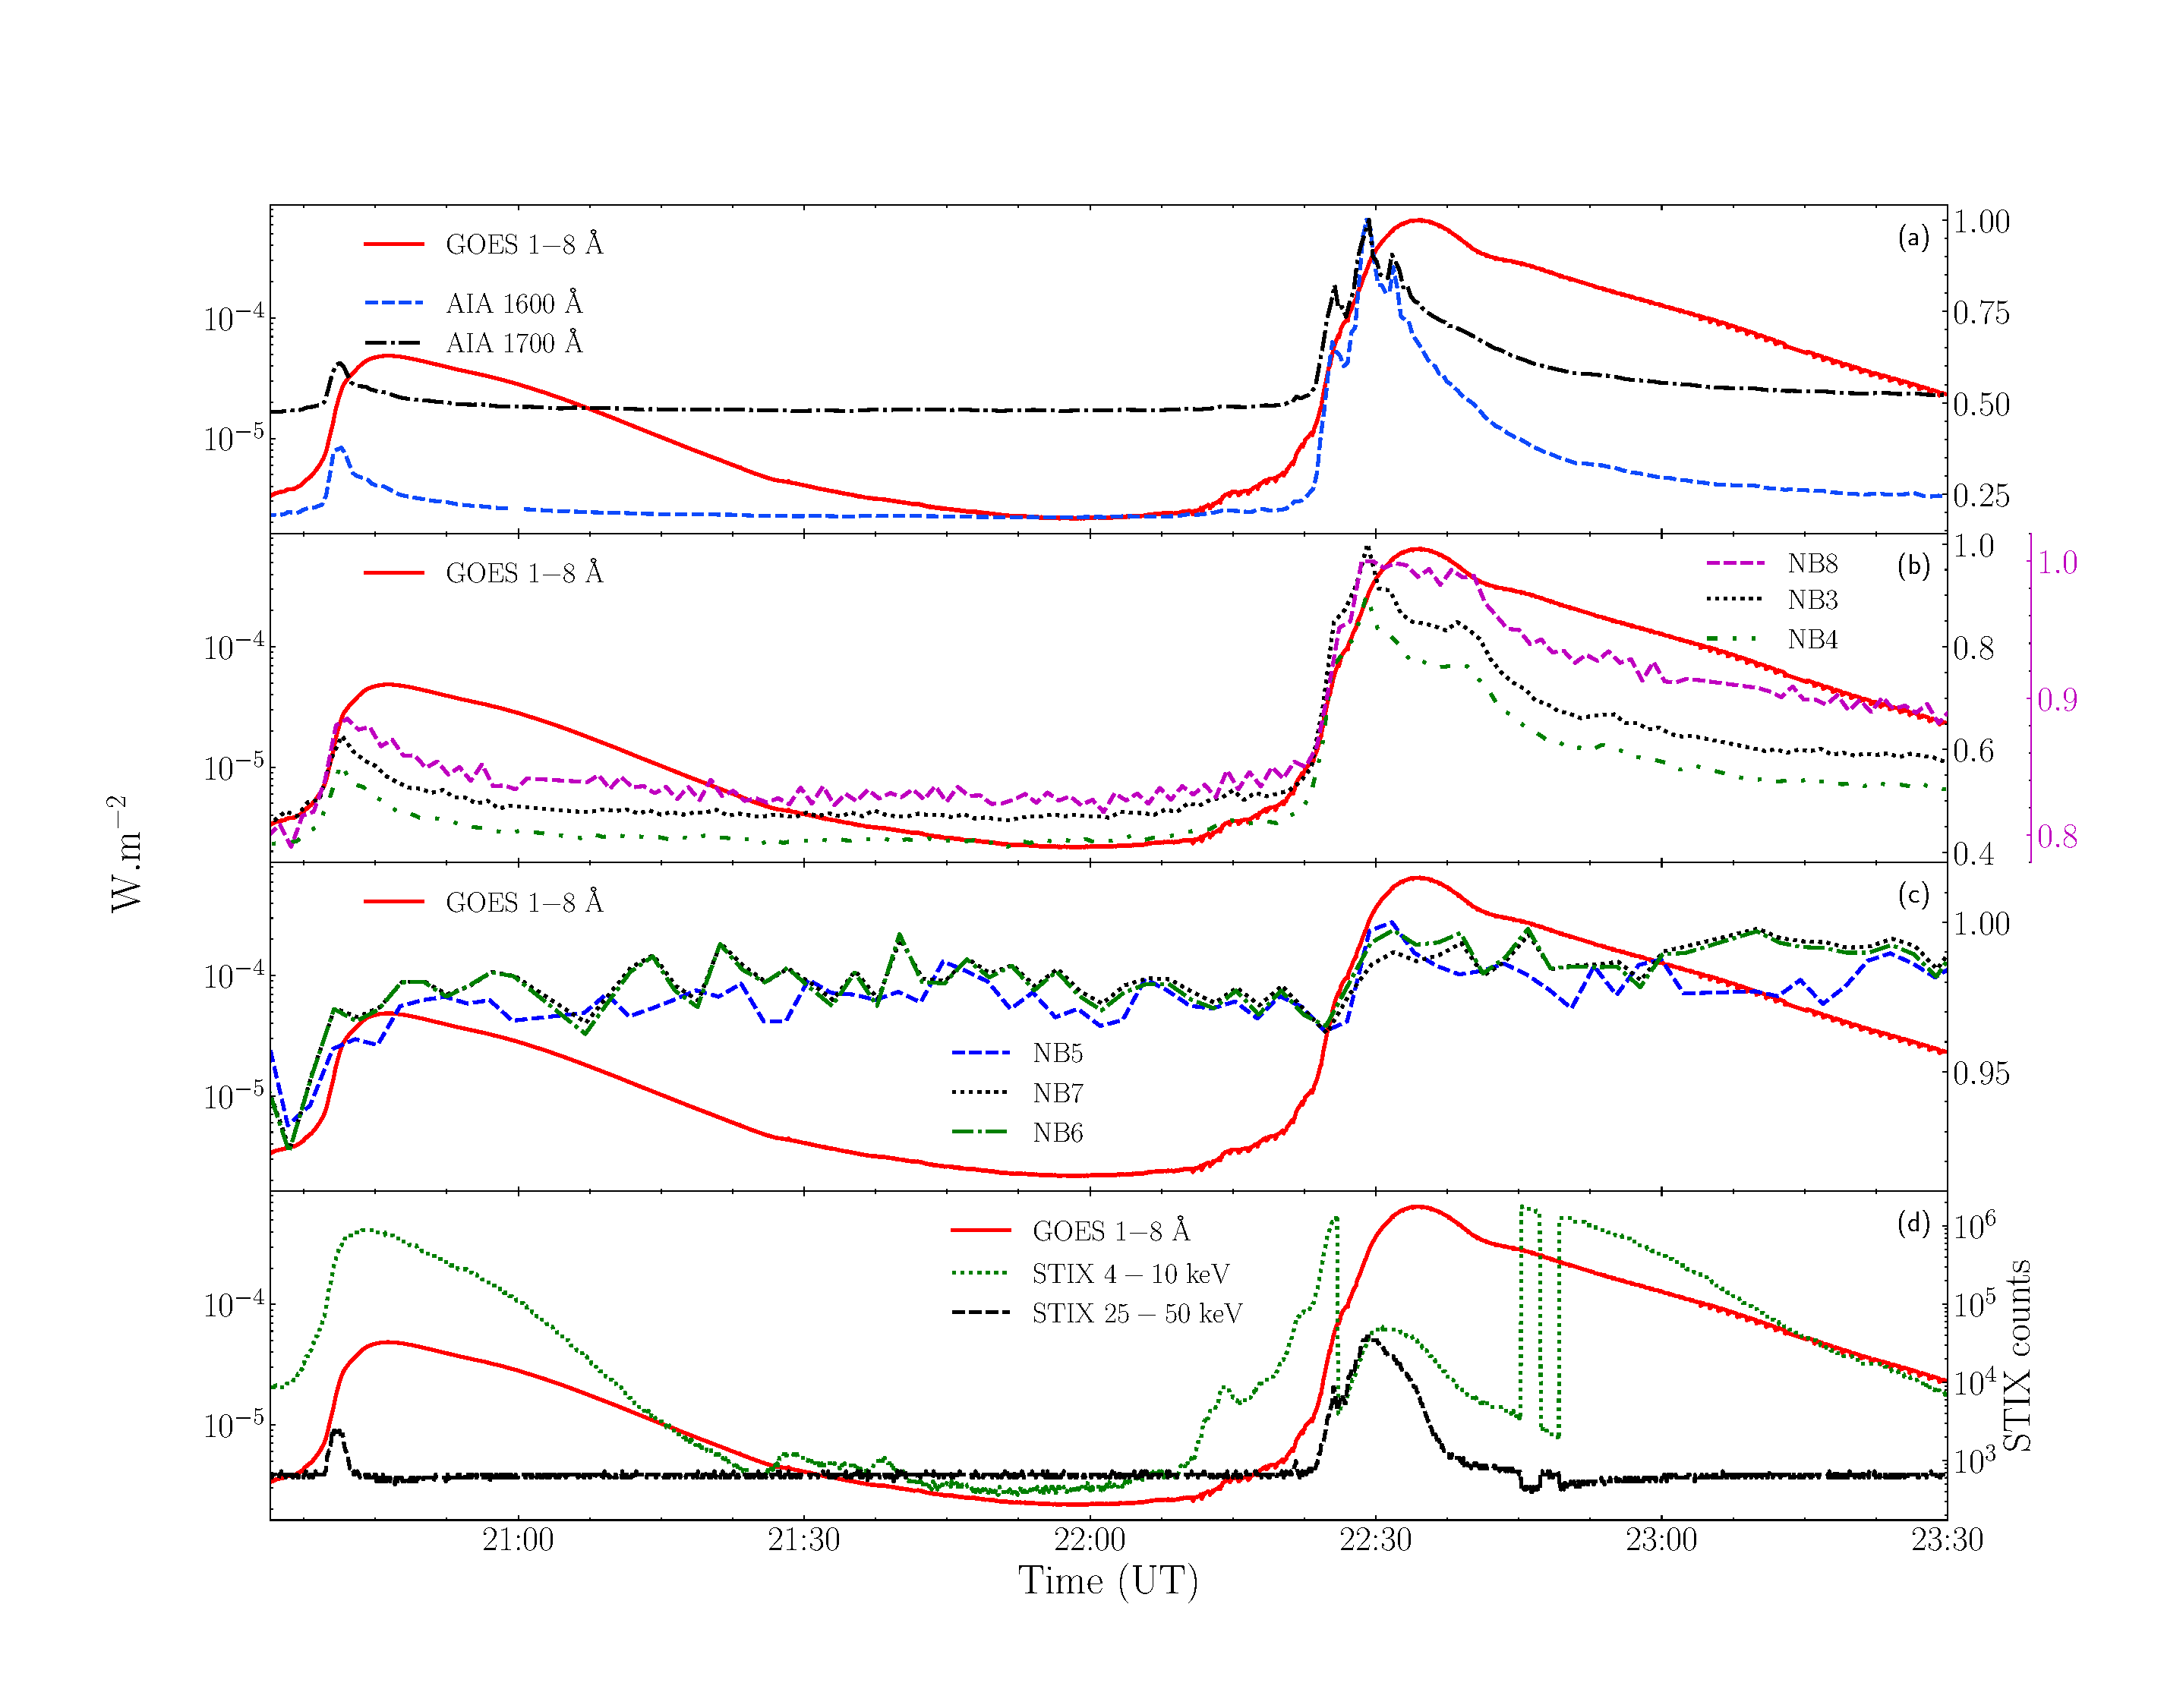
\includegraphics[width=0.8\textwidth,trim={2.3cm 2.5cm 1cm 4.5cm},clip]{lc_full_suit_contour.pdf}
    \caption{Light curves from the whole RoI FoV of \suit~observations compared with AIA, {\it GOES} and STIX observation for the two flares.}
    \label{fig:flare_full}
\end{figure}
%%%%%%%%%

The X6.3 flare provides a good example of the response of the local plasma environment to the flare in the Near Ultraviolet (NUV) regime in 200 {--} 400 nm. The flare peaked around $\sim$ 22:34 UT in the {\it GOES} observation. Images from six narrow band (NB) channels of \suit~ are shown in Fig.~\ref{fig:flare_nb3_peak} top panel at around $\sim$ 22:28-22:29 UT. This is at the peak of the NB3 (\ion{Mg}{2} k 279.6 nm) channel, as observed by \suit. The 60\% peak intensity contour of the NB3 intensity is marked with the black line in all figures of Fig.~\ref{fig:flare_nb3_peak} top panel. From the figure, we also see a similar structure in the NB4 (\ion{Mg}{2} h 280.3 nm) and NB8 (\ion{Ca}{2} h 396.9 nm). No similar structure is observed in the other continuum channels of Fig.~\ref{fig:flare_nb3_peak} top panel.

In Fig.~\ref{fig:flare_nb3_peak} bottom panel, we show the flare observations by \suit~ at their respective peaks. Again, we see very similar structures in NB3, NB4, and NB8. NB3 and NB4 peak at almost the same time $\sim$ 22:29 UT. Although NB8 shows a similar structure, the peak intensity of NB8 is observed slightly later around $\sim$ 22:29:41 UT. The peak intensities of the other continuum NB channels are observed progressively later. The NB5 (Red wing of the Mg window) peaks around $\sim$ 22:32:41 UT. Faint signatures of flare brightening are observed in NB5, marked with red arrows in Fig.~\ref{fig:flare_nb3_peak} bottom panel. No such signatures are observed as clearly in NB6 and NB7. Both of these channels peak around $\sim$ 22:28 UT.

%%%%%%%%%
\begin{figure}[ht!]
    \centering
    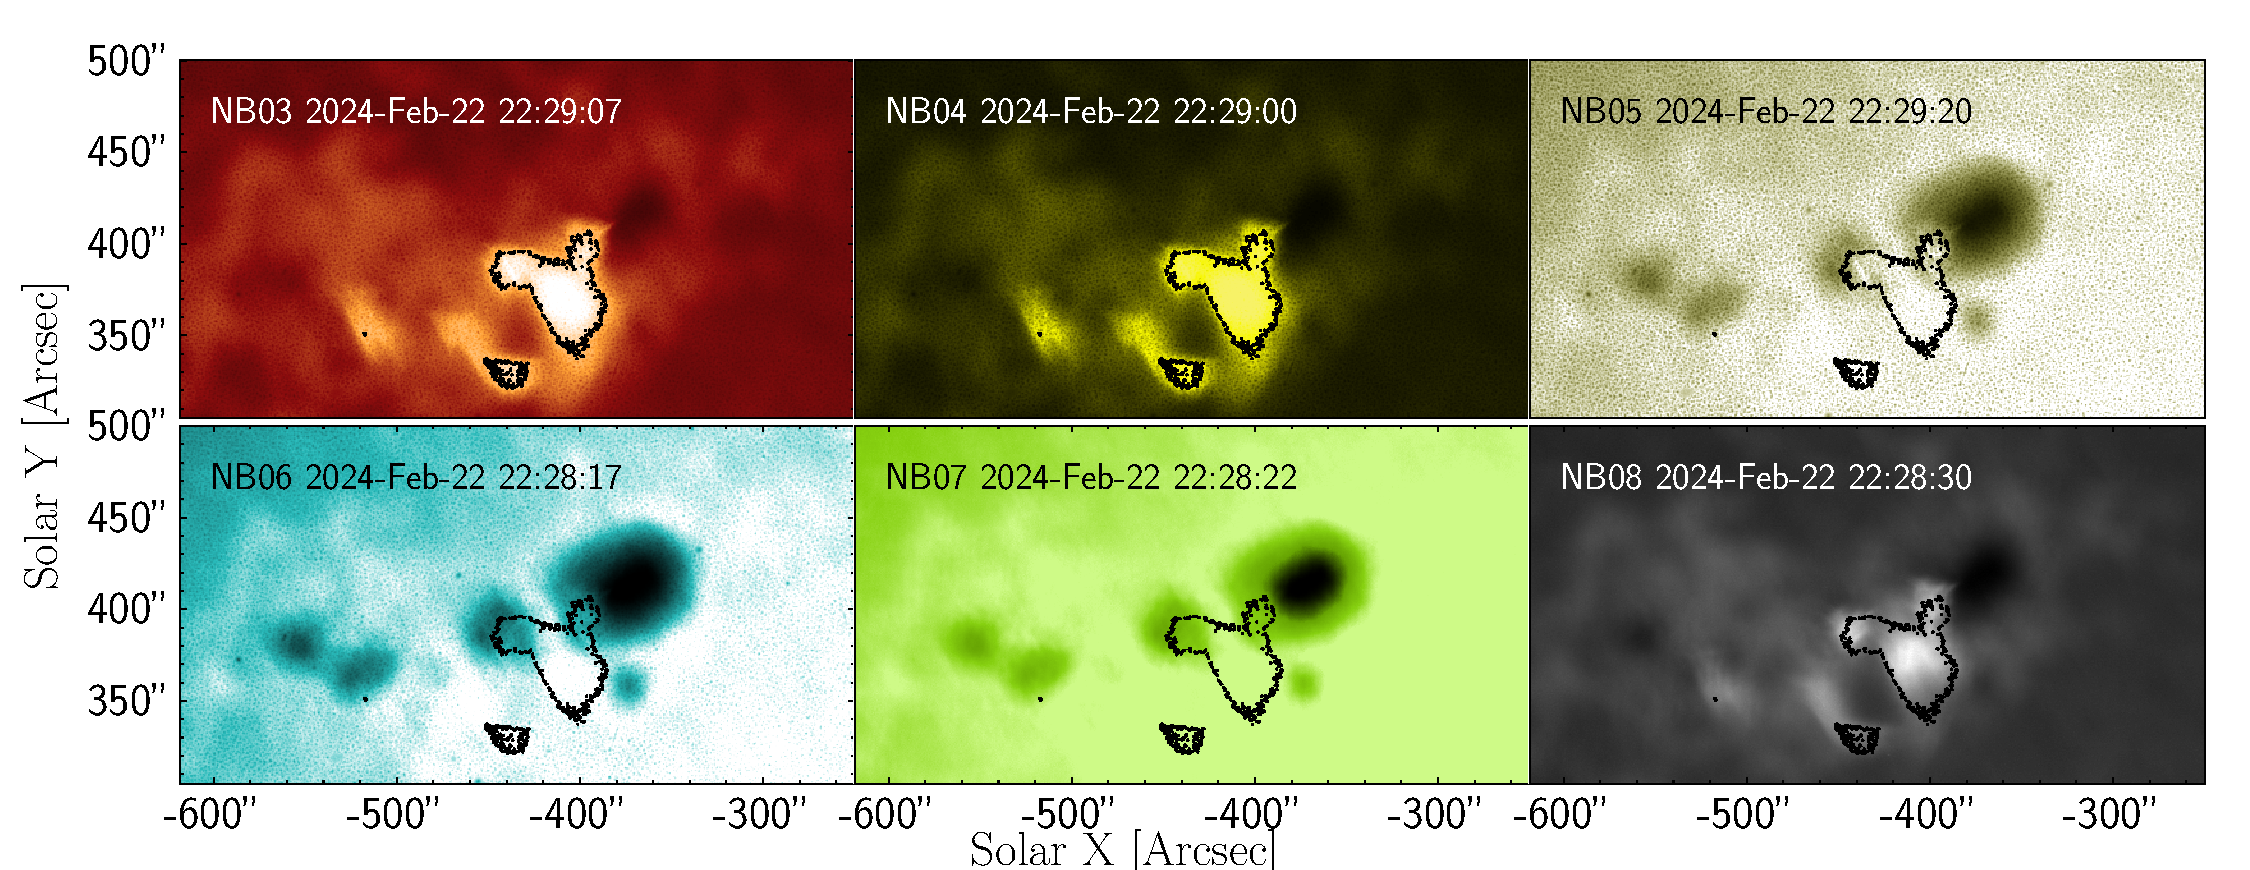
\includegraphics[trim={0cm 0.65cm 0cm 0cm},clip,width=0.5\textwidth]{suit_roi_nb3_peak.pdf} \\
    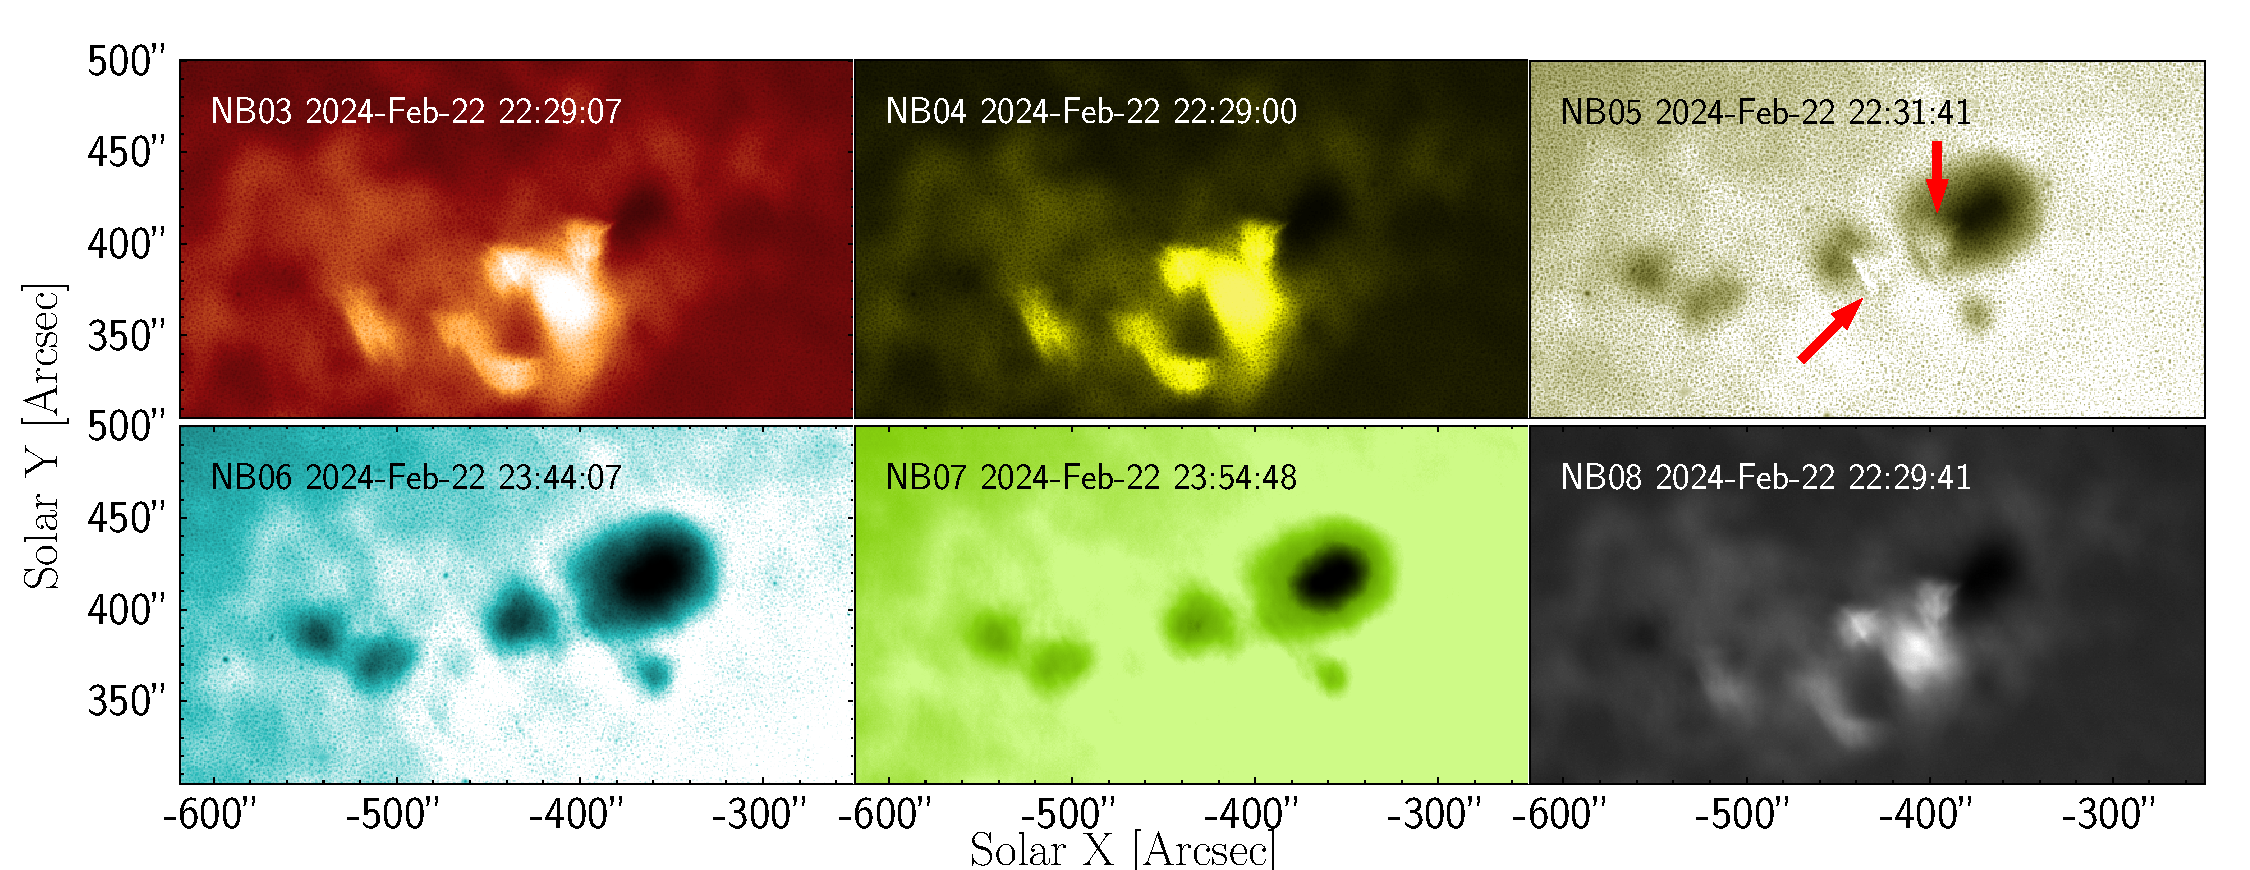
\includegraphics[width=0.5\textwidth]{suit_roi_all_peak.pdf}
    \caption{\suit~observations of the flare from various NB filters. Top panel: during NB3 peak. Bottom panel: During the peak of individual bands.}
    \label{fig:flare_nb3_peak}
\end{figure}
%%%%%%%%%

In Fig.~\ref{fig:flare_lc_suit}, we plot the light curve of the event to compare the observations across various bands. The AIA and \suit~ light curves in Fig.~\ref{fig:flare_lc_suit} are calculated by adding the counts within the region of 60\% peak intensity contour of NB3 (shown in Fig.~\ref{fig:flare_nb3_peak} top panel), after co-aligning and registering the AIA and \suit~observations and normalizing them to the peak intensity. In Fig.~\ref{fig:flare_lc_suit}.a, we show the GOES 1 {--} 8 {\AA} light curve in comparison to AIA 1600 {\AA} and AIA 1700 {\AA}. The AIA 1600 and 1700 {\AA} light curve peaks around $\sim$ 5 minutes earlier than the {\it GOES} peak. 

In Fig.~\ref{fig:flare_lc_suit}.b, we show the GOES 1 {--} 8 {\AA} light curve in comparison to the NB3, NB4 and NB8 light curves. All the NB light curves behave remarkably similarly. The vertical dotted black line across all the panels in Fig.~\ref{fig:flare_lc_suit} denotes the peak intensity in NB3. NB3, NB4, and NB8 peaks around $\sim$ 22:29 UT, which is very similar to AIA 1600 {\AA} and 1700 {\AA}. We also plot the {\it GONG}-H$\alpha$ light curve from the \suit~contour region. The {\it GONG} light curve also peaks at around $\sim$ 22:29 UT. Both NB8 and {\it GONG}-H$\alpha$ shows less contrast variation in the light curve than NB3 and NB4.

We show the GOES 1 {--} 8 {\AA} light curve in comparison to the NB5 (Red wing of the Mg lines, blue dashed), NB6 and NB7 continuum channels in Fig.~\ref{fig:flare_lc_suit}.c. NB5 shows signs of flare response, although much weaker than NB3, NB4 and NB8. NB5 peaks around $\sim$ 22:31 UT, about $\sim$ 3 minutes later than NB3. Similar traits were observed from the images also, as pointed out in Fig.~\ref{fig:flare_nb3_peak} bottom panel and the accompanying discussions. More interestingly, NB6 and NB7 do not show the hallmark sign of a flare light curve, i.e. gradual increase and decrease in the intensity. These bands exhibit a slow but steady rise in intensity after the flare. Finally, in Fig.~\ref{fig:flare_lc_suit}.d, we show the {\it GOES} 1 {--} 8 {\AA} light curve in comparison to the STIX hard and soft X-ray light curve. The hard X-ray peaks around a similar time around $\sim$ 22:29 UT, similar to NB3, NB4 and AIA 1600 and 1700 {\AA}.

%%%%%%%%%
\begin{figure}[ht!]
    \centering
    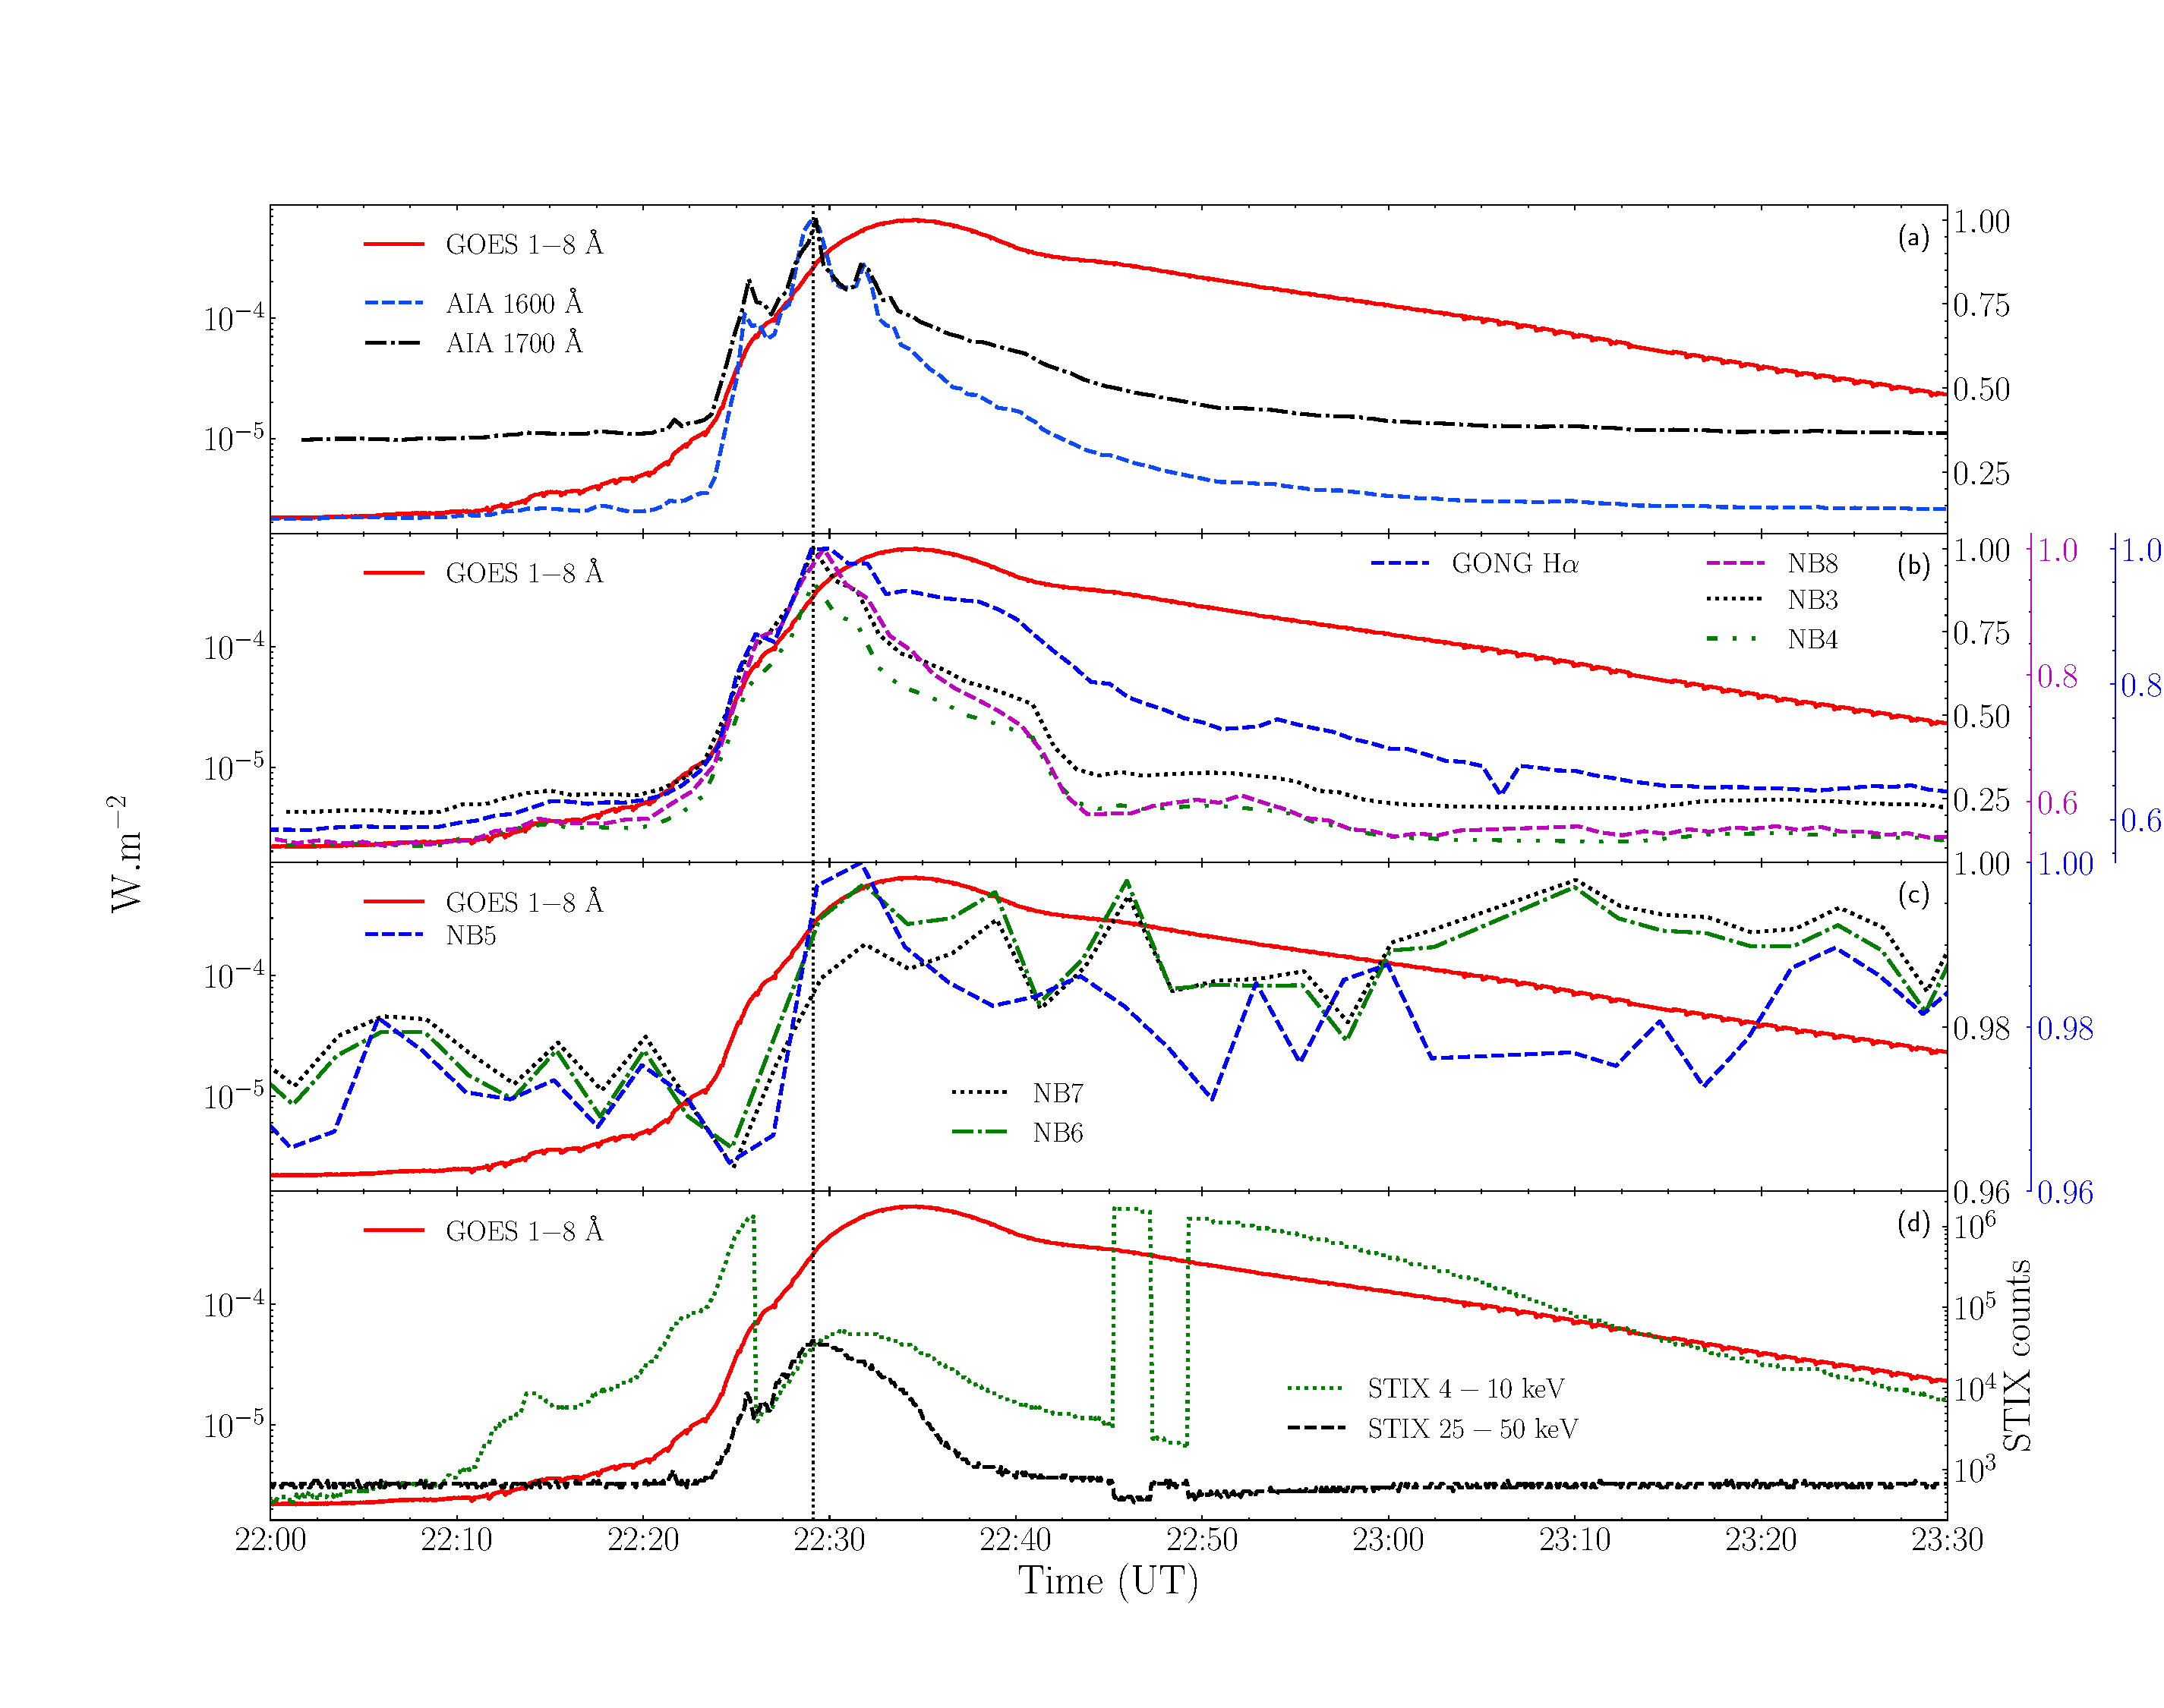
\includegraphics[width=0.8\textwidth,trim={2.3cm 2.5cm 0cm 4.5cm},clip]{lc_suit_contour.pdf}
    \caption{Light curves from the pixels within intensity contour picked from \suit~and co-aligned AIA observations. The NB4 light curve in the second panel is offset by -0.1 from NB3 for better visibility. The vertical dotted dark line marks the flare's peak in NB3 observation.}
    \label{fig:flare_lc_suit}
\end{figure}
%%%%%%%%%

%%%%%%% ############# %%%%%%%
\subsection{XSM-spectra}\label{sec:xsm}
%%%%%%% ############# %%%%%%%

The Solar X-ray monitor on {\it Chandrayan-2}\citep[{\it Chandrayan-2}/XSM,][]{xsm} provides sun as a star soft X-ray spectra in 1{--}15 keV with 1s cadence and significantly better spectral resolution (180 eV at 5.9 keV) compared to STIX (1 keV ar 5.9 keV). The high spectral and temporal resolution allows us to measure the change in elemental abundances over the duration of the flares. XSM observed both flares with coverage in both impulsive and decay phase. The existing studies with XSM has successfully studies the thermal and elemental abundance evolution of various flares \citep{mondal21,kkepa23,nama23}.

Both the M and X-class flares were observed by XSM. The XSM 1{--}8 {\AA} light curves are plotted in Fig.~\ref{fig:xsm-obs} top panel. The red shaded region marks the time window where the Be filter was inserted to prevent saturation. There are periodic gaps in the data due to periodic lunar occultation. We show the spectra obtained by XSM in Fig.~\ref{fig:xsm-obs} bottom panel, during various phases of the flare. The violet spectra at 22:33 UT is near the flare peak, and shows a sharp decrease below 3 keV due to the insertion of the Be filter to avoid saturation. Various Mg, Al, S and Si lines are visible in the pre-flare spectra. In stark contrast during impulsive and peak of the flare we see strong signatures of Ca, Ar and Fe. Due to the uncertainty of the spectra during the Be window observation in $<~3~\mathrm{keV}$ regime, we fit the spectra beyond 3 keV throughput this analysis. We fit the spectra with the XSPEC model {\it chisoth}, which uses a wide range of pre-calculated spectra to fit the observed spectra (For more details please refer to the appendix of \cite{mondal21}).

%%%%%%%%
\begin{figure}[ht!]
\centering
    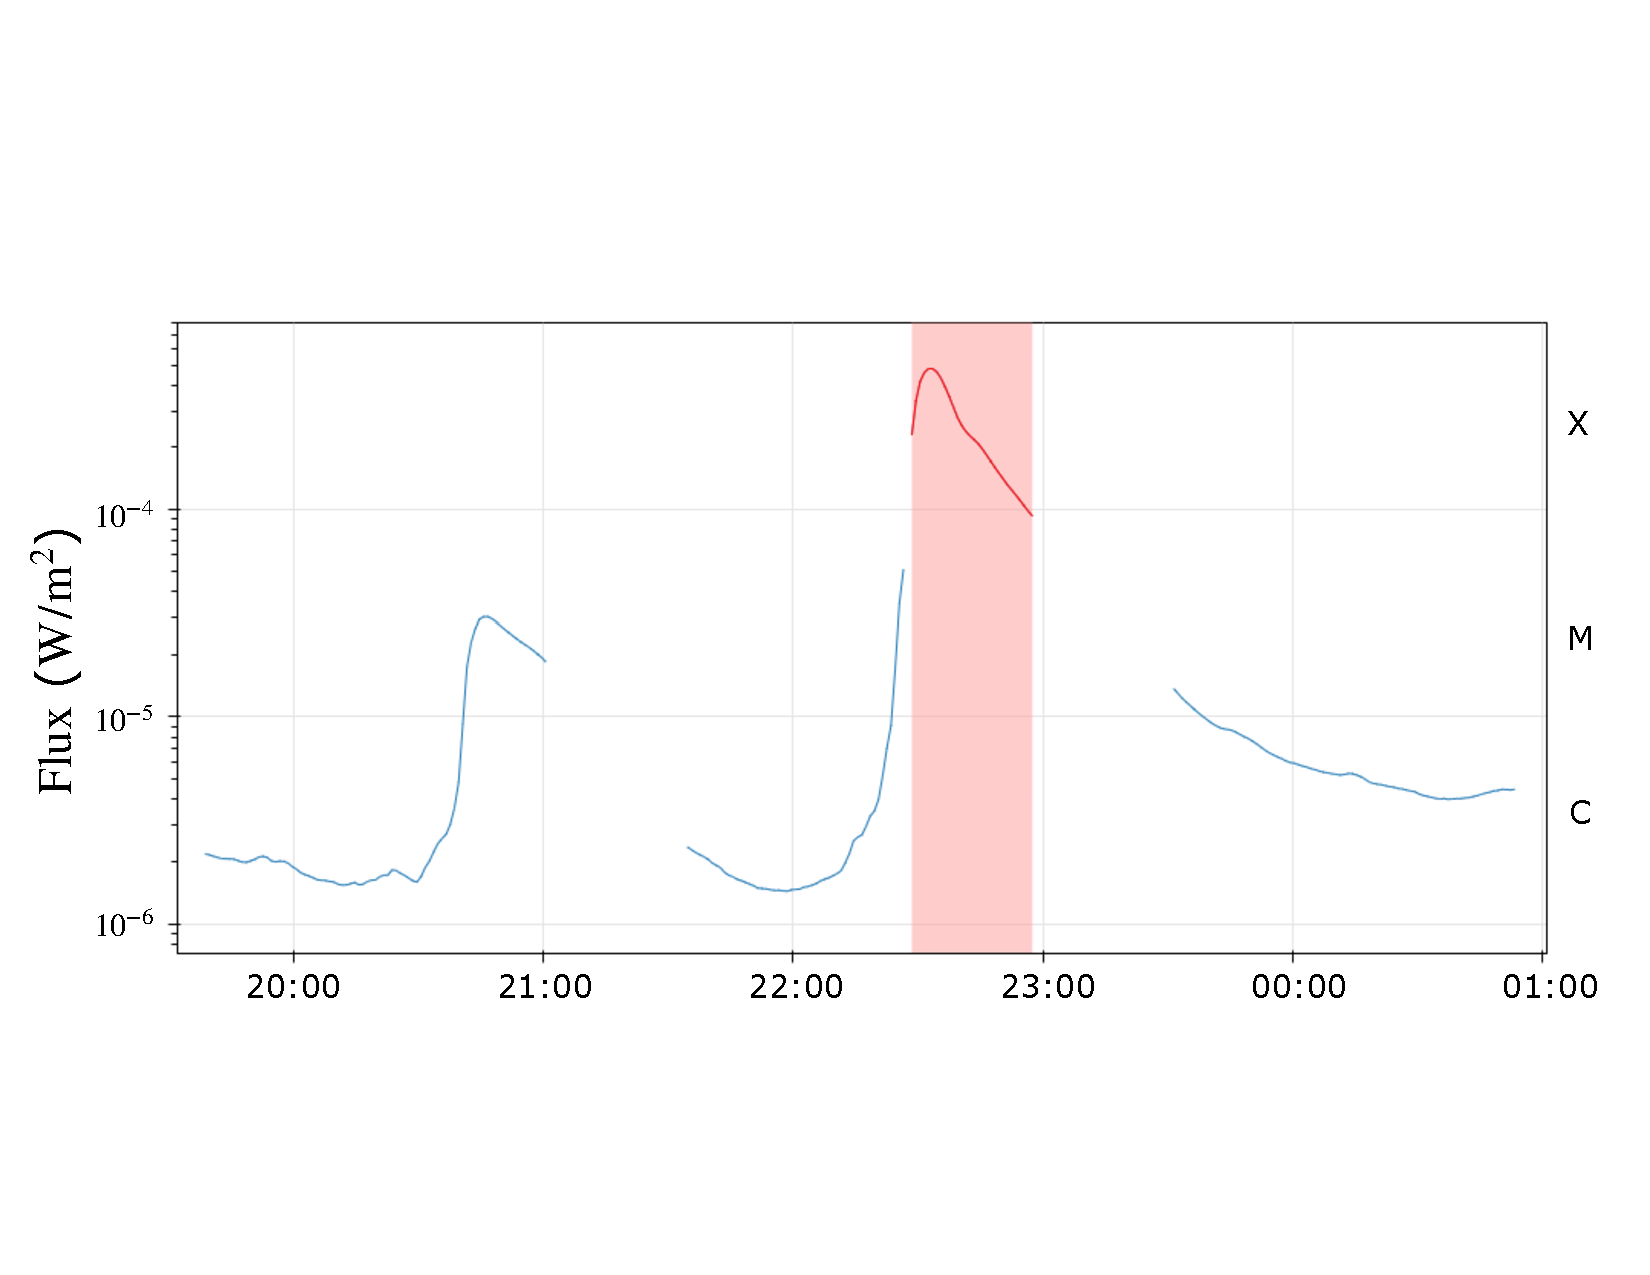
\includegraphics[trim={0.5cm 3.3cm 0.8cm 4cm}, clip, width=0.76\textwidth]{xsm_lc.pdf} \\
    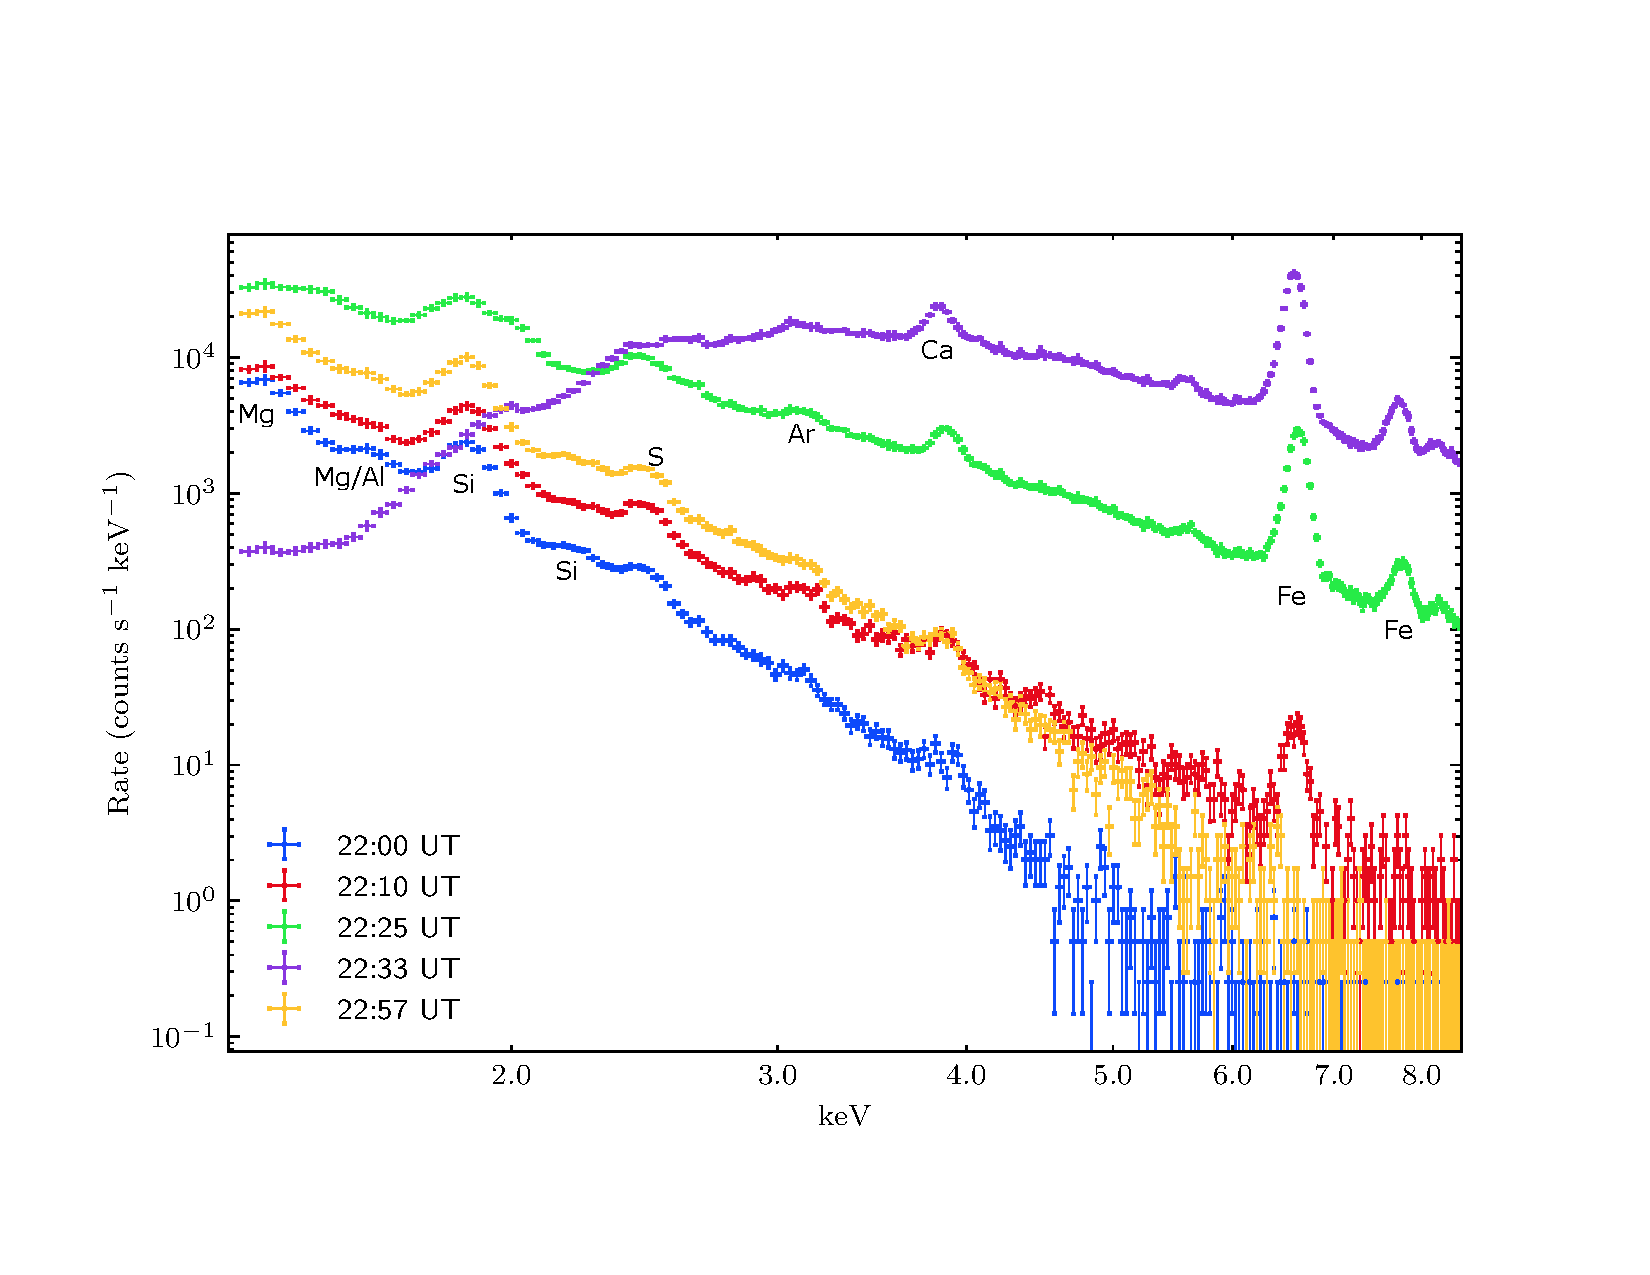
\includegraphics[trim={1.8cm 2.5cm 3cm 3cm},clip,width=0.75\textwidth]{xsm_spec.pdf}
    \caption{Top panel: XSM observation of the two flares. The red shaded region marks the window when the Be filter was inserted. Bottom panel: X-ray spectra during various phases of the flare. The violet spectra is during the soft X-ray peak of the flare and shows a sharp decrease in the intensity below 3 keV. This is due to the insertion of Be filter to avoid saturation.}
    \label{fig:xsm-obs}
\end{figure}
%%%%%%%%

%%%%%%% ############# %%%%%%%
\subsubsection{Fitting XSM spectra}\label{sec:xsm-fit}
%%%%%%% ############# %%%%%%%

The observed soft X-ray spectra from the flaring plasma can be modelled by an isothermal plasma characterized by various parameters {\it e.g.} temperature, emission measure and abundance of various elements. As alluded earlier, we use the `{\it chisoth}' model \citep{mondal21} to fit the observed spectra from XSM. The `{\it chisoth}' model uses CHIANTI atomic database \cite{chianti} to calculate spectra for individual elements over a large temperature grid and stores as tables. The model includes elements from H (Z=1) to Zn (Z=30). The spectra of individual elements are calculated over a wide temperature range (0.3 {--} 50 MK). These modelled spectra of various elemental abundance over a wide temperature range are loaded in XSPEC and added with varying weights to fit the observed spectra. The Total model spectrum is given by  $$I_{mod}(T)~=~EM\sum_{X}I_{X}(T)N_{X}$$`EM' is the volume emission measure, $N_{X}$ is the abundance of element X relative to H and $I_{X}(T)$ is the modelled spectrum of element X at temperature T. The fit is done in a recursive process by minimizing the chi-squared between the observed and modelled spectra.

We initially used an isothermal model to fit the spectra. One of the key observations we make is a presence of systematic residual around the Fe complex around $\sim$ 6.5 keV. This is illustrated in the top panel of Fig.~\ref{fig:xsm_fit} top panel, where there is an excess visible in the blue side of the Fe line complex at $\sim$ 6.7 keV. \cite{mithun22} could not explain this systematic excess with multithermal DEM distributions. One of the possible explanation of this excess flux is Fe fluorescence emission. There have been observations of Fe line fluorescence at 6.4 keV (Fe K$\alpha$) and 7.06 keV (Fe K$\beta$) \citep{neupert67,doscheck71,bai79,tanaka84,parmar84,phillips12} using high-resolution X-ray spectra from Bent Crystal Spectrometer on-board Solar Maximum Mission \citep[Bent/{\it SMM},][]{bent,smm} and Yokoh \citep{yokoh} mission. Previous studies have suggested that this emission arises from the excitation of low ionization state Fe in the Photosphere either via the X-ray from the flaring plasma \citep{bai79} or directly from the non-thermal electron beam \citep{phillips73}. The Fe K$\alpha$ fluorescence is usually dependent on the position on the solar disk \citep{parmar84}. The emergent Fe K$\alpha$ emission suffers significant absorption and scattering along the line of sight, which increases with increasing heliocentric angle, resulting in a decrease in the observed intensity. For our event, the flaring region is near the disk center making the Fe K$\alpha$ fluorescence a valid candidate for explaining the excess. We added a Gaussian component to the `{\it chisoth}' model to get better fit (see Fig.~\ref{fig:flare_obs} bottom panel).

We add a Gaussian line component to our fit at 6.4 keV to explore the possibility of the excess flux arising from Fe K$\alpha$ fluorescence. We find that this fits the observed spectra better than previous instances, as demonstrated in Fig.~\ref{fig:xsm_fit} bottom panel. The K$\alpha$ emission would arise from the X-ray emission from the flaring regions having energies $>$ 7.12 keV, the K edge of Fe, exciting the Fe atoms in the Photosphere. We show the intensity of the fitted Fe 6.4 keV component excess (blue solid line), in comparison to the fitted flux in 7.12 {--} 8.5 keV (green dot-dashed line) in Fig.~\ref{fig:fe_excess} top panel. For reference, {\it GOES} 1{--}8 {\AA} soft X-ray flux (red dotted line) and STIX 25 {--} 50 keV Hard X-ray flux (black dashed line) are overplotted. STIX Hard X-ray is a fair representative of the non-thermal electron flux deposited into the foot points. In the bottom panel, the light curve fitted Fe 6.4 keV excess Gaussian component is plotted with the lightcurve from the bright kernels marked with the two boxes in Fig.~\ref{fig:flare_nb3_peak} bottom panel. In both panels, the peak time of the Fe excess (blue solid line), STIX hard X-ray (black dashed line) and NB5 brightness from box 1 (dotted magenta line) are marked with vertical lines.

%%%%%%%%%%
\begin{figure}[ht!]
    \centering
    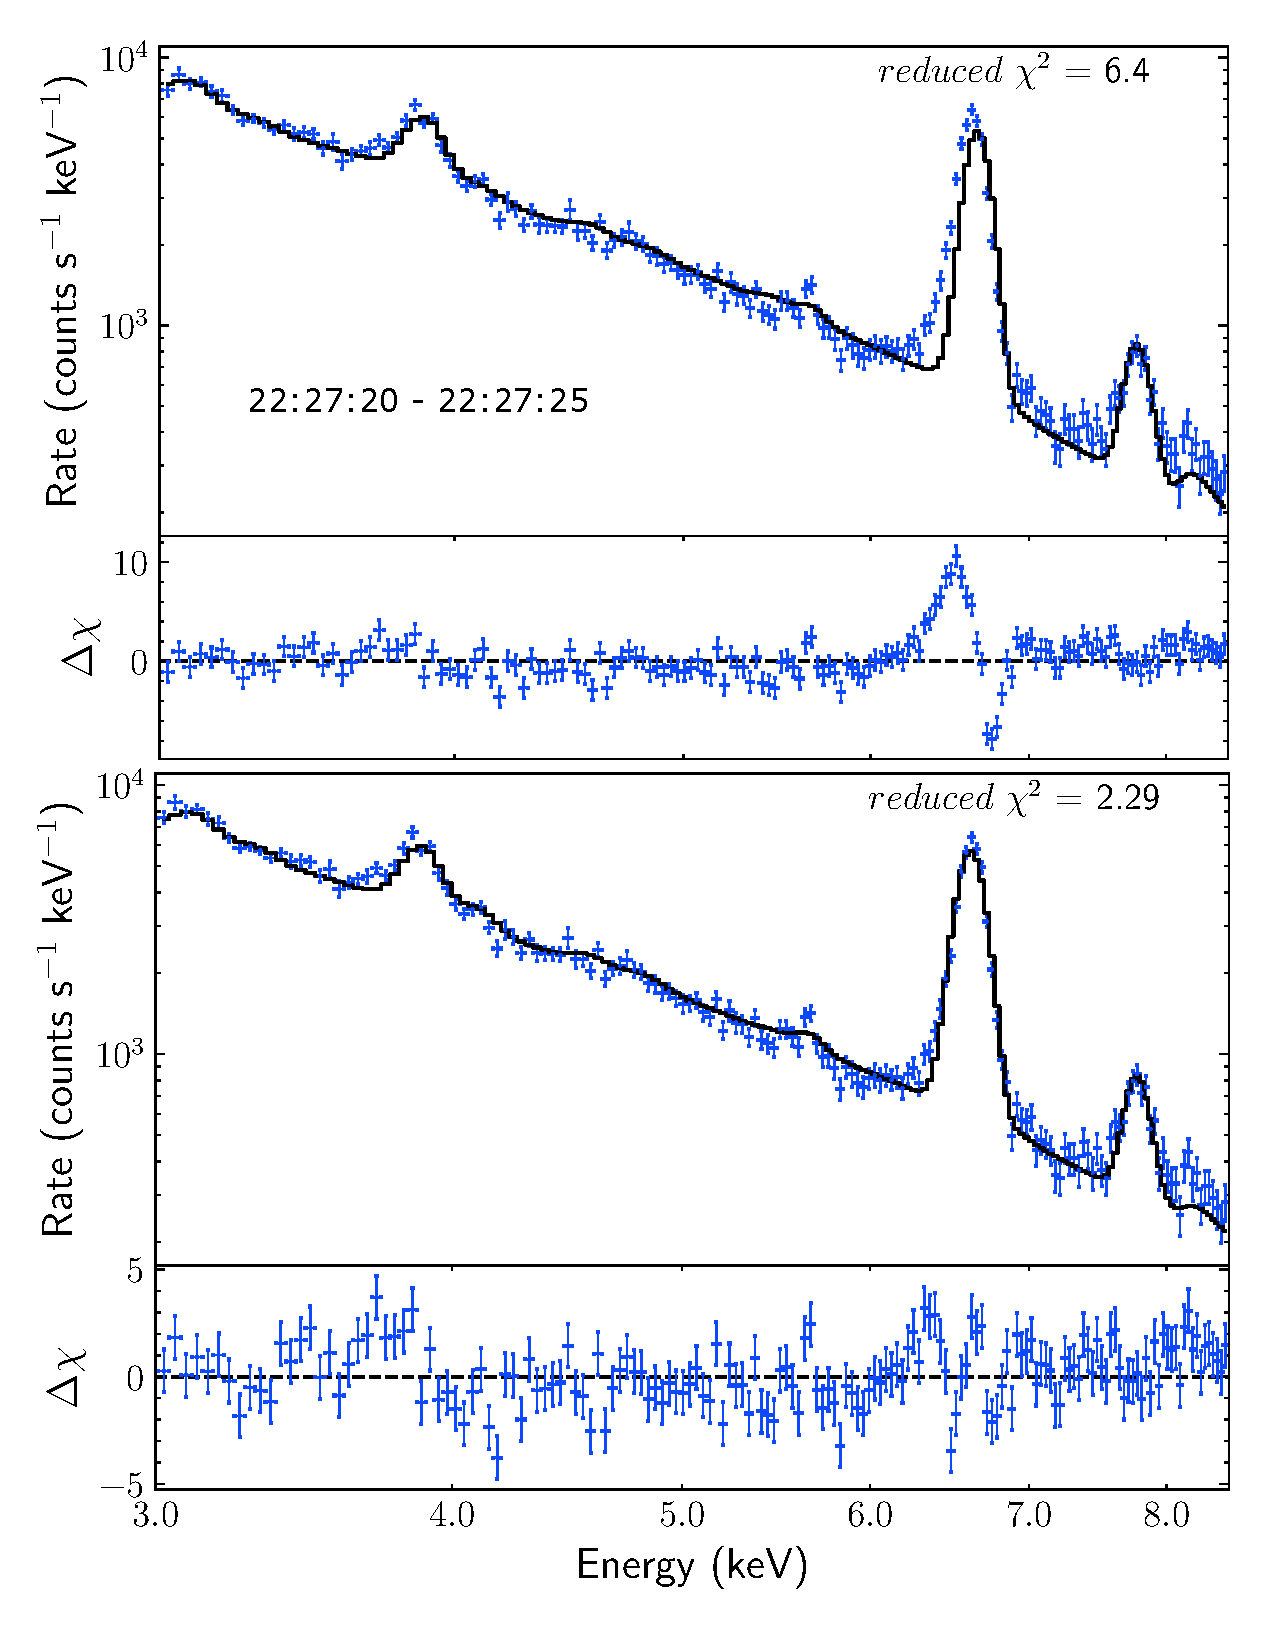
\includegraphics[trim={0.5cm 1cm 0.5cm 0.7cm}, clip, width=0.77\textwidth]{xsm_fit.pdf}
    \caption{XSM spectra in 3 {--} 8.5 keV binned between 22:27:20 {--} 22:27:25 UT. Top panel shows the fit with ``chisoth+chisoth" model. Bottom panel shows the same spectra fitted with ``chisoth+chisoth+gaussian" model.}
    \label{fig:xsm_fit}
\end{figure}
%%%%%%%%%%

%%%%%%%%%%
\begin{figure}[ht!]
\centering
    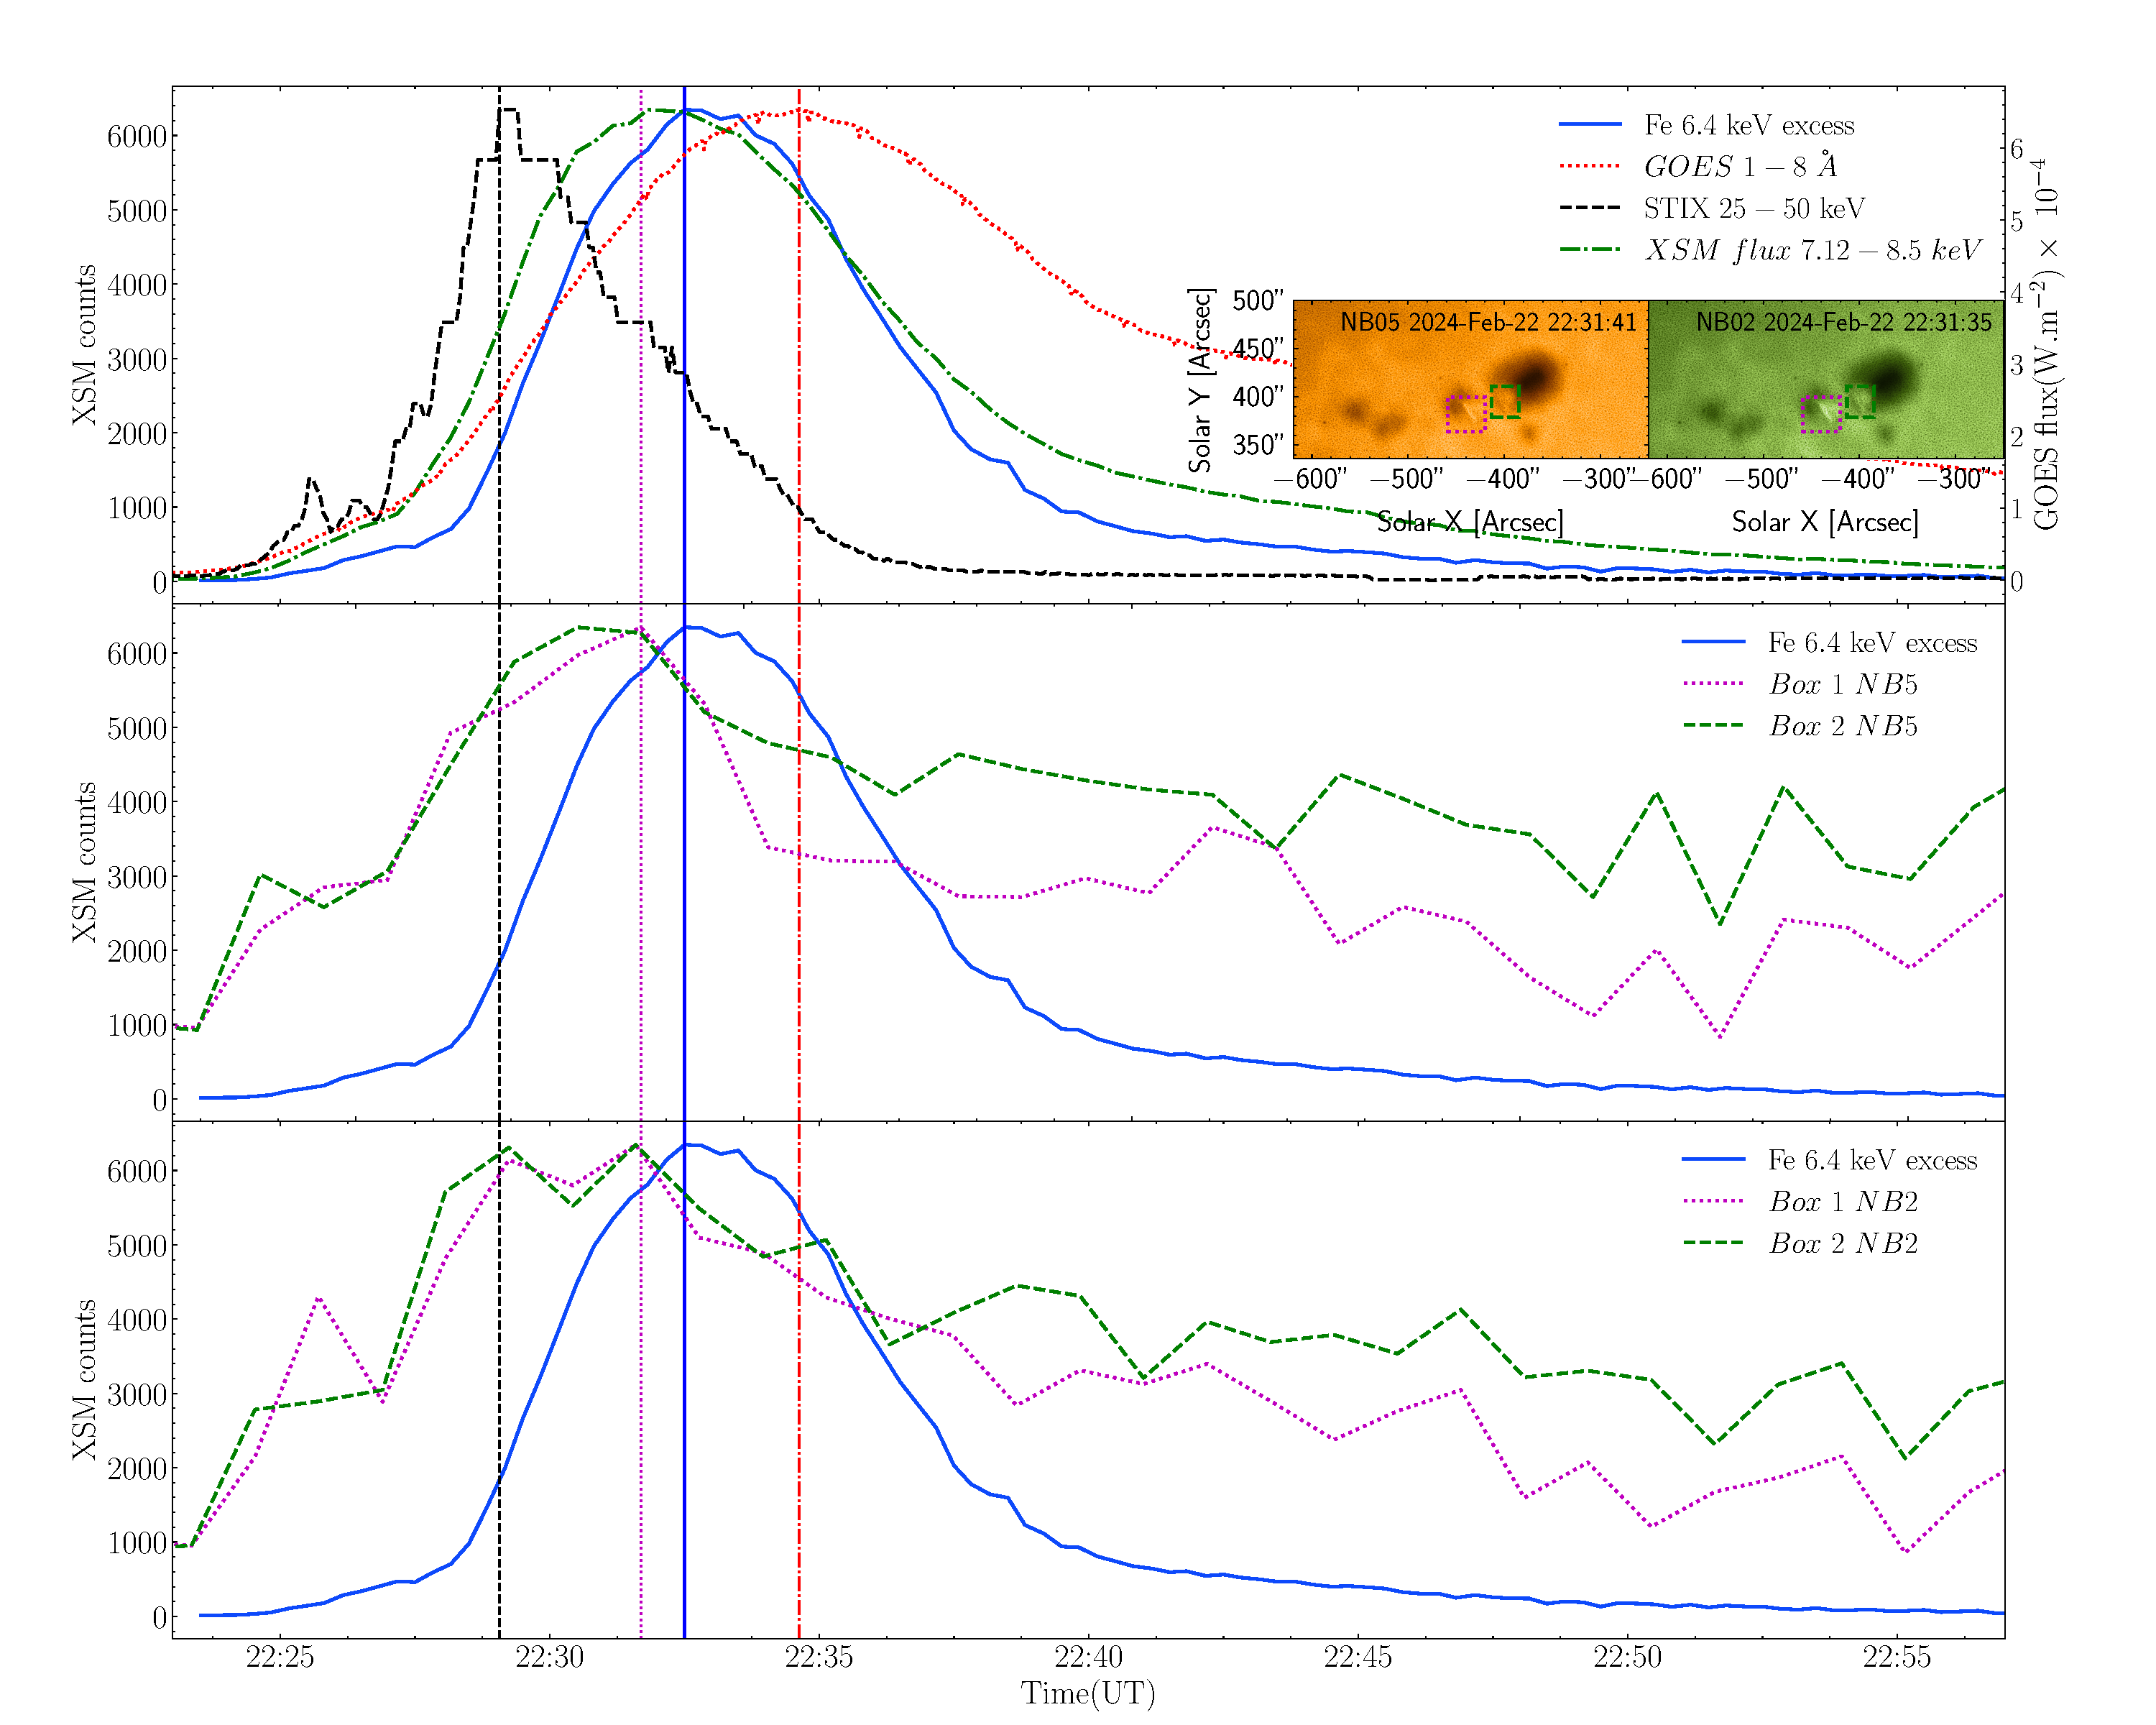
\includegraphics[trim={1.3cm 0.1cm 0.3cm 1.2cm}, clip, width=0.95\textwidth]{fe_excess_4.pdf}
    \caption{Fe excess emission from 6.4 keV(blue solid) in comparison to STIX 25-50 keV(black dashed), GOES 1 {--} 8 $\AA$ (dotted red) and XSM 7.12 {--} 8.5 keV (green dot-dashed) light curve.}
    \label{fig:fe_excess}
\end{figure}
%%%%%%%%%%

%%%%%%% ############# %%%%%%%
\subsection{Discussion}\label{sec:dis1}
%%%%%%% ############# %%%%%%%

This section reports the \suit~narrow band imaging of the first localized flare by the onboard flare detection algorithm. We report the observation in NB3 (\ion{Mg}{2} k 279.6 nm), NB4 (\ion{Mg}{2} h 280.3 nm), NB8 (\ion{Ca}{2} h 396.9 nm) and the continuum channels NB5 (Red wing of \ion{Mg}{2}), NB6 and NB7. For both the flares, the NB3, NB4 and NB8 peak around the same time as AIA 1600 and 1700 {\AA}. For the X6.3 flare, NB3, NB4 behave very similarly to NB8 within the NB3 intensity contour (see Fig.~\ref{fig:flare_lc_suit}.b). But the NB8 peak over the whole active region is much broader compared to the NB3 and NB4 light curves (see Fig.~\ref{fig:flare_full}). This implies that NB8 behaves differently in other parts of the active region.

The NB5 observes the continuum that is usually attributed as the Balmer continuum. There have been previous studies where Photospheric metal lines went into emission and affected the Balmer continuum \citep{heinzel14,kleint17}. The dominant contribution would still be the Balmer continuum. \cite{reetika21} attributed the brightening in the SJI 2832 {\AA} continuum for a mini flare to direct signature of electron beams. \cite{kowalski19} showed for one event, that the SJI 2832 {\AA} continuum enhancement and several Phototspheric absorption lines going into emission can be attributed to significant Photospheric heating. The entire 2832 {\AA} window of IRIS had several \ion{Fe}{2} and \ion{Cr}{2} lines which are usually observed as absorption lines, in emission. Curiously enough, this observation was also made in a bright umbral flare kernel, similar to the current event. As there was no {\it IRIS} scan of the umbral brightening visible in NB5, unfortunately, we can not comment on the spectral nature of the bright kernel.

We see an excess around the 6.5 keV Fe complex from the XSM observations which can be fitted with a single Gaussian. From Fig.~\ref{fig:fe_excess}, the Fe excess light curve (blue solid line) behaves very similar to the soft X-ray flux beyond the Fe K edge at 7.12 keV (green dot-dashed line). The excess also shows no correlation with the STIX 25 {--} 50 keV hard X-ray flux (black dashed line), illustrating no significant contribution from the non-thermal electron flux. This suggests that the excess flux seen around 6.4 keV Fe complex arises from the Fe fluorescence from the flaring X-ray. If we assume the penumbral brightening observed in this flare to be similar as observed by \cite{kowalski19}, the bright kernels observed in NB5 mainly arises from a plethora of \ion{Fe}{2} lines. The flaring X-ray beyond Fe K edge (7.12 keV) photoionizes the Fe in the Photosphere, giving rise to both \ion{Fe}{2} lines in the red wing of \ion{Mg}{2}, along with the observed Fe fluorescence by XSM. 

We see a similar brightening in NB2, the blue wing of the Mg window. The light curve of the brightening of the blue wing of Mg is shown in Fig.~\ref{fig:fe_excess} third panel. The light curve shows peak at both hard X-ray peak and later on closer to Fe excess component peak. This possibly shows both Photospheric and Chromospheric components from the NB2. Further investigation and modelling is required to comment on the local plasma parameters that would produce the bright kernels observed in both NB5 and NB2, with the relative timing within themselves and also in comparison to the various energies in X-ray.

The other interesting observation is the rise in the continuum intensity, specifically in NB6 and NB7 as the flares happen. We can see a steady rise in the continuum intensity after the M and X class flare (see Fig.~\ref{fig:flare_full}). For the X6.3 flare, we do see some signature of the flare in NB5, although it peaks about $\sim$ 5 minutes later compared to NB3 and NB4. The photospheric nature of the NB5 continuum explains the 5-minute delay of the peak from NB3. We see the flare peak in sequential order of formation height NB3 and NB4 (\ion{Mg}{2}, 22:29 UT) and NB8 (\ion{Ca}{2}) $\Longrightarrow$ NB5 (Photospheric continuum, 22:32:41 UT). We are observing the increase in continuum intensity from 283.2 nm to 388 nm. The consistent increase in continuum intensity is happening across the Balmer jump ($\lambda$~=~364.5 nm).

%%----------------------------------------------------
\section{X1 flare observed on Dec 31st, 2023} \label{sec:dec_31st}
%%----------------------------------------------------


\clearpage
%
\chapter{First flares observed from {\suit}}\label{c:chap8}
\chaptermark{Solar flare energy}
\begin{quote}
{\em ~~~~~~~This thesis chapter originally appeared in the literature as} \\
{authors,
{\em journal reference info}}
\end{quote}
\justifying

%%----------------------------------------------------
\section{Introduction} \label{sec:intro}
%%----------------------------------------------------

The Solar Ultraviolet Imaging Telescope onboard {\it Aditya-L1} \citep[{\it Aditya-L1}/SUIT,][]{article,ghosh16,adityal1,suit_main} provides a targeted probe into the Chromosphere and Transition region. It provides continuous full-disk and Region of Interest (RoI) coverage of the Sun in eleven pass bands. The details of these bands are provided in chapter~\ref{c:chap3} Tab.~\ref{tab:science_filters}. The eight narrow bands provide coverage across the \ion{Mg}{2} k and h lines, \ion{Ca}{2} h line, the CN band, red and blue wing of the \ion{Mg}{2} window and parts of the NUV continuum. As alluded earlier, this provides unprecedented coverage of the Chromospheric and Transition region structure of solar flares.

The {\it Aditya-L1} was launched on September 2nd, 2023. The first light observations were made on December 5th, 2023 while the payload was still in cruise phase. For the majority of the cruise phase the payload only operated in the 2k synoptic mode, i.e. it only captured continuous (2k $\times$ 2k) observations in NB4 (\ion{Mg}{2} h line) with one minute cadence. The L1 insertion was carried out on January 6th, 2024. Following that the payload also started taking (4k $\times$ 4k) observations in all eleven science filters. Various components of the flare detection algorithm were progressively turned on. In this chapter we discuss some of the initial flare observations made by SUIT. The first flare triggered by the flare detection algorithm was a X6.3 flare from north-west corner of the disk on February 22nd, 2024, which was also observed by several other instruments {\it e.g.} {\it SDO}/AIA, {\it IRIS}, {\it SO}/STIX. During the cruise phase, SUIT also observed a X1 flare from the south-east limb of the Sun on December 31st, 2023. We only have observations in the NB4 (\ion{Mg}{2} h line) channel for this flare. But this provides us with an unprecedented view of post-flare loops and possibly reconnection slingshot in the \ion{Mg}{2} line. Subsequent portions of this chapter will be divided into two parts, where we discuss the observations of these two flares separately.

%%----------------------------------------------------
\section{X6.3 flare observed on Feb 22nd, 2024} \label{sec:feb_22nd}
%%----------------------------------------------------

NOAA AR 13590 was visible on the north-east of the Solar disk on February 22, 2024. The AR was around a large sunspot in a cluster of sunspots, accompanied by a complex magnetic field structure. The active region flared multiple times during the same day, including an X1.7 flare that peaked around $\sim$ 06:32 UT, an M4.8 flare that peaked around $\sim$ 20:46 UT and an X6.3 flare that peaked $\sim$ 22:34 UT . \suit~is equipped with an onboard flare detection algorithm. Once the flare detection algorithm flags a flare and localizes the position of the flare on the detector, the program sequence prioritizes reading a fixed smaller Region of Interest (RoI) around the location for fast, higher cadence observation (for further details, please refer to \cite{flare_det}). The X6.3 flare was one of the first flares to be localized by the on-board flare detection algorithm. \suit~did not observe the X1.7 flare because, during that time, the payload was off-pointed to verify the stellar calibration program sequences. The flares were also observed by {\it SDO}/AIA, {\it SO}/STIX. {\it IRIS} observed the eastern edge of the X6.3 flare ribbons in a small [66\arcsec,62\arcsec] field of view (FoV) with a 4 step raster and 15 s raster cadence.

We show the light curve arising from the whole RoI observation in comparison to {\it GOES} flux in Fig.~\ref{fig:flare_full}. In Fig.~\ref{fig:flare_full}.b, we plot the AIA 1600 {\AA} (dashed blue line) and AIA 1700 {\AA} (black dot-dashed line), in comparison to the {\it GOES} 1 {--} 8 {\AA} light curve (Solid red line) for both the flares. In Fig.~\ref{fig:flare_full}.b, we show the GOES 1 {--} 8 {\AA} light curve in comparison to the NB3 (\ion{Mg}{2} k 279.6 nm, black dotted), NB4 (\ion{Mg}{2} h 280.3 nm, green dot-dashed) and NB8 (\ion{Ca}{2} h 396.85 nm, magenta dashed) light curves. NB4 light curve is offset from NB3 by -0.1 for better visibility. The NB8 light curve exhibits lower contrast and does not show a sharp peak compared to NB3 and NB4. The other interesting trend is exhibited by the continuum channels NB5, NB6 and NB7 in Fig.~\ref{fig:flare_full}.c, as a conspicuous rise in the continuum intensity is seen after both flares. In Fig.~\ref{fig:flare_full}.d we plot the {\it GOES} 1 {--} 8 {\AA} light curve in comparison to the STIX hard (25 {--} 50 keV, black dashed) and soft (5 {--} 10 keV, green dotted) X-ray light curve. The hard X-ray observation from STIX peaks at a time similar to that of NB3, NB4, and NB8.

%%%%%%%%%
\begin{figure}[ht!]
    \centering
    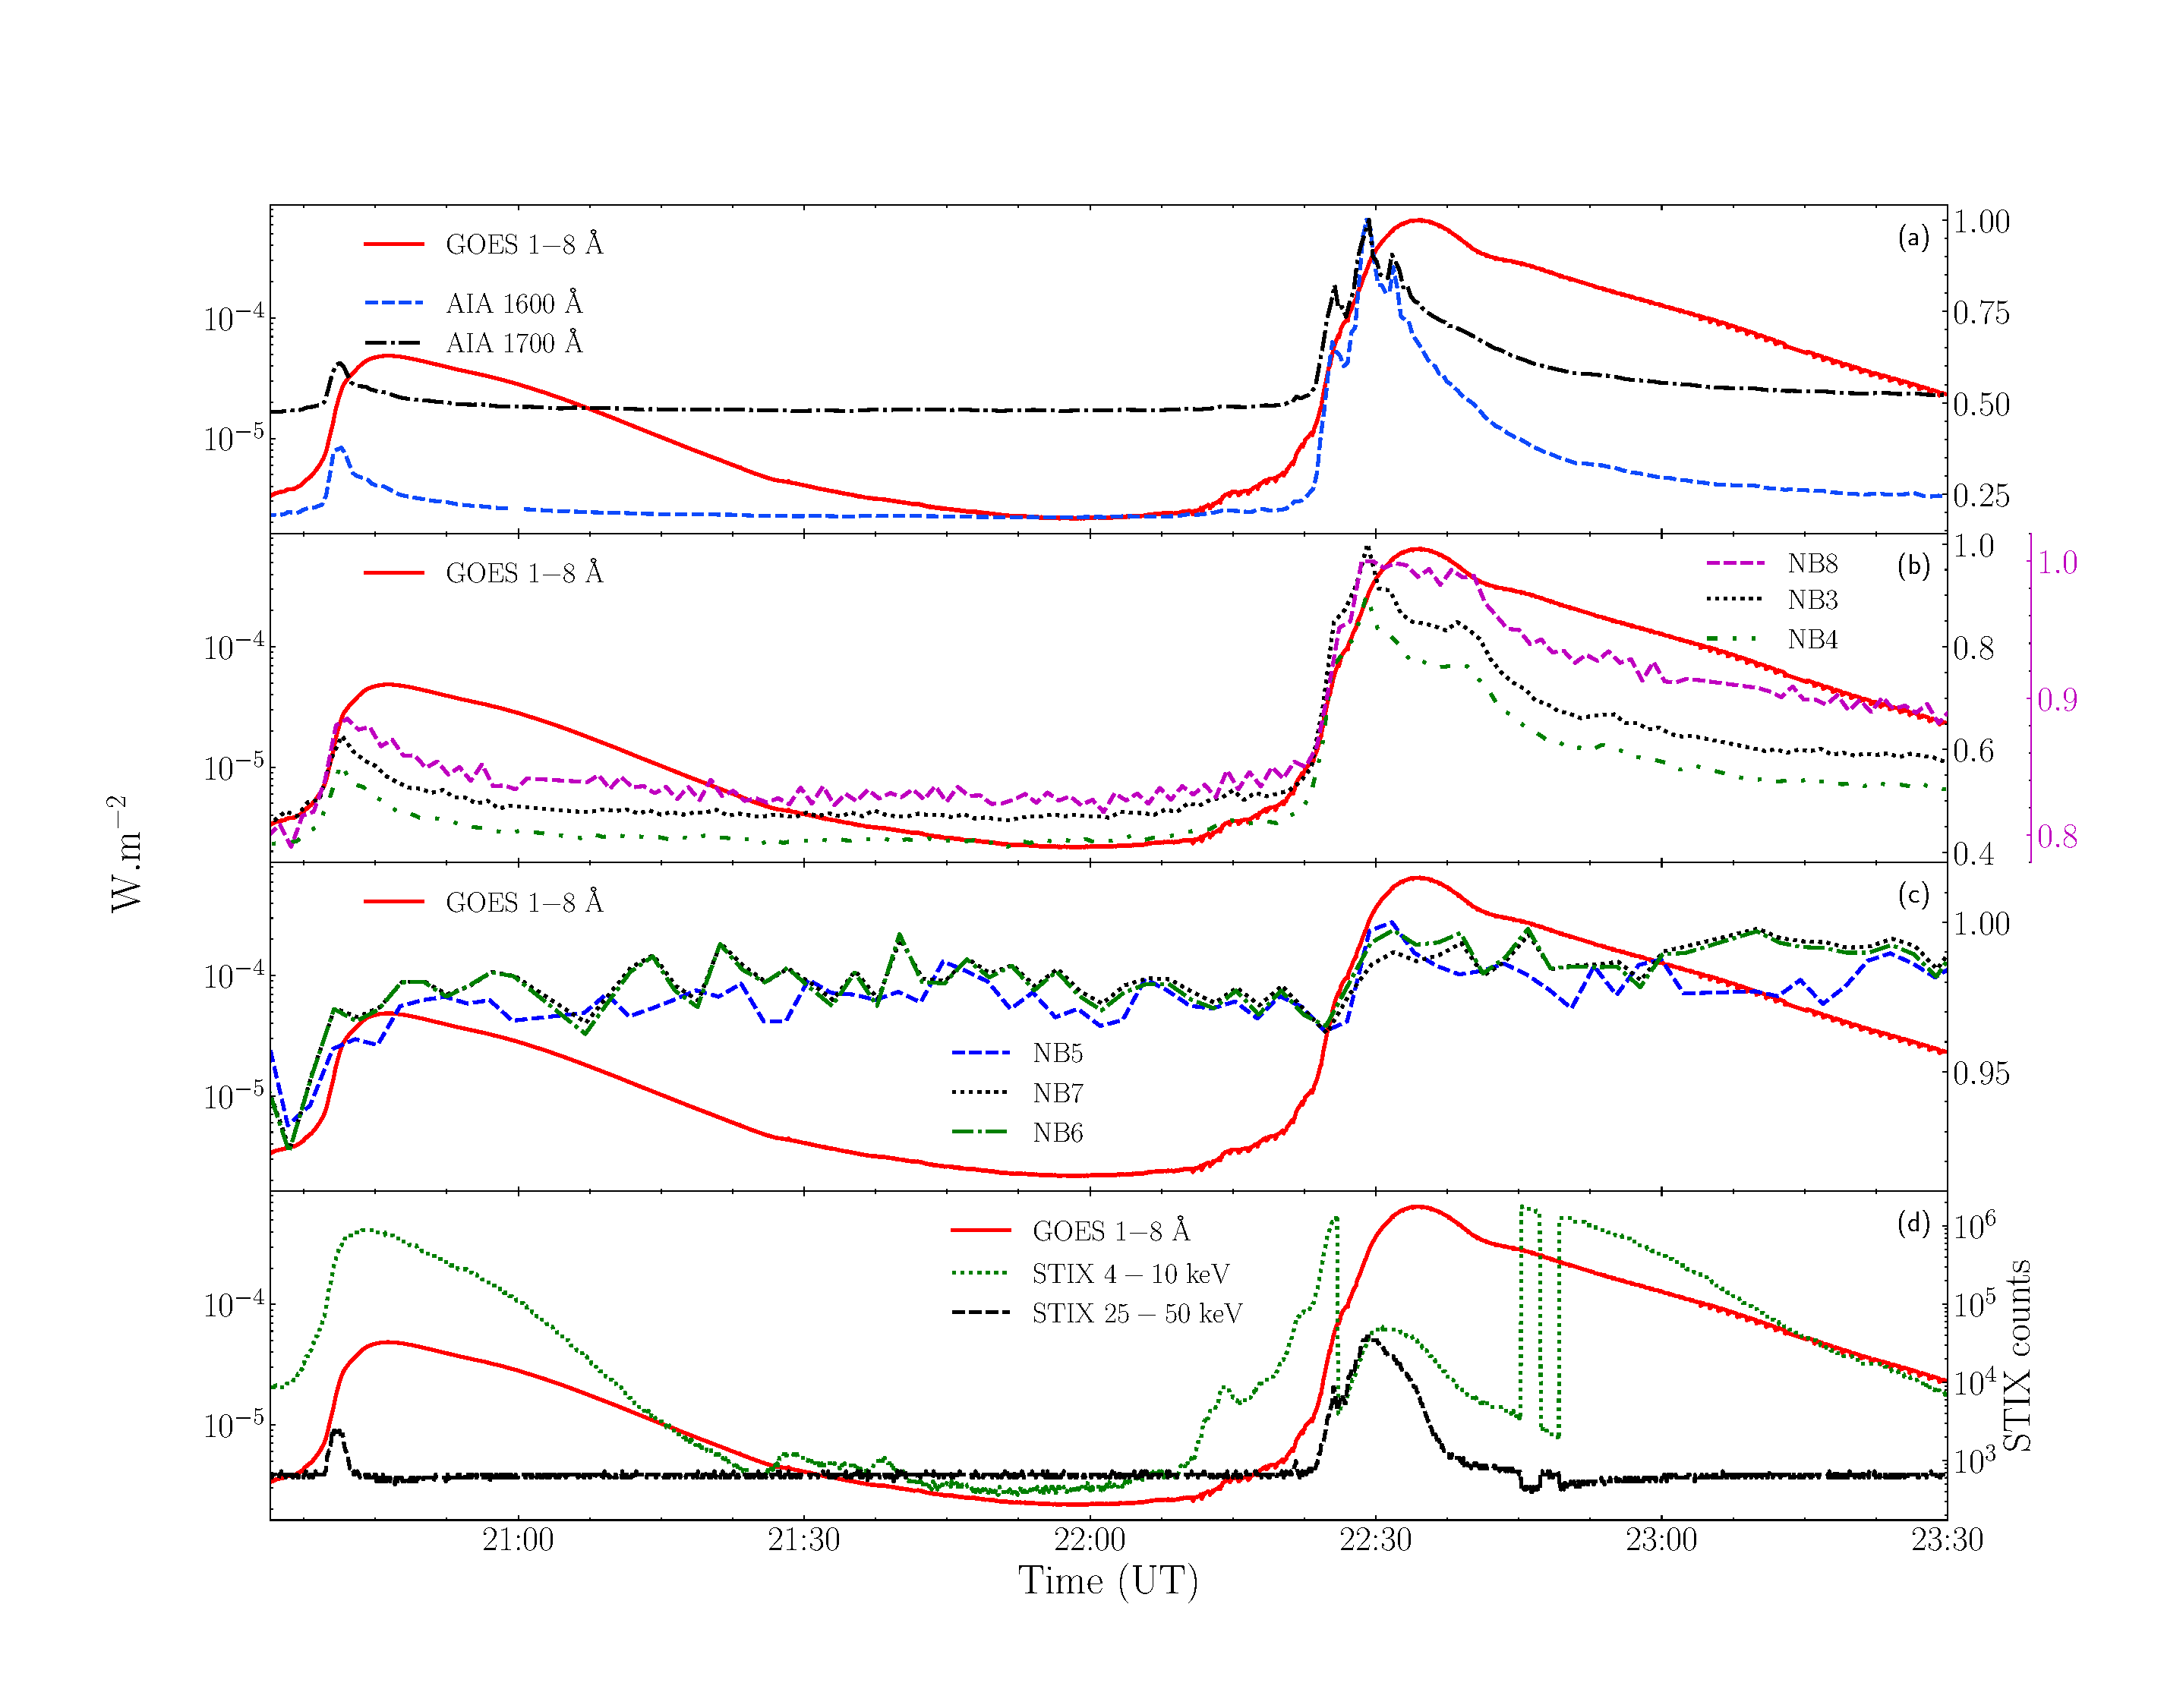
\includegraphics[width=0.8\textwidth,trim={2.3cm 2.5cm 1cm 4.5cm},clip]{lc_full_suit_contour.pdf}
    \caption{Light curves from the whole RoI FoV of \suit~observations compared with AIA, {\it GOES} and STIX observation for the two flares.}
    \label{fig:flare_full}
\end{figure}
%%%%%%%%%

The X6.3 flare provides a good example of the response of the local plasma environment to the flare in the Near Ultraviolet (NUV) regime in 200 {--} 400 nm. The flare peaked around $\sim$ 22:34 UT in the {\it GOES} observation. Images from six narrow band (NB) channels of \suit~ are shown in Fig.~\ref{fig:flare_nb3_peak} top panel at around $\sim$ 22:28-22:29 UT. This is at the peak of the NB3 (\ion{Mg}{2} k 279.6 nm) channel, as observed by \suit. The 60\% peak intensity contour of the NB3 intensity is marked with the black line in all figures of Fig.~\ref{fig:flare_nb3_peak} top panel. From the figure, we also see a similar structure in the NB4 (\ion{Mg}{2} h 280.3 nm) and NB8 (\ion{Ca}{2} h 396.9 nm). No similar structure is observed in the other continuum channels of Fig.~\ref{fig:flare_nb3_peak} top panel.

In Fig.~\ref{fig:flare_nb3_peak} bottom panel, we show the flare observations by \suit~ at their respective peaks. Again, we see very similar structures in NB3, NB4, and NB8. NB3 and NB4 peak at almost the same time $\sim$ 22:29 UT. Although NB8 shows a similar structure, the peak intensity of NB8 is observed slightly later around $\sim$ 22:29:41 UT. The peak intensities of the other continuum NB channels are observed progressively later. The NB5 (Red wing of the Mg window) peaks around $\sim$ 22:32:41 UT. Faint signatures of flare brightening are observed in NB5, marked with red arrows in Fig.~\ref{fig:flare_nb3_peak} bottom panel. No such signatures are observed as clearly in NB6 and NB7. Both of these channels peak around $\sim$ 22:28 UT.

%%%%%%%%%
\begin{figure}[ht!]
    \centering
    \includegraphics[trim={0cm 0.65cm 0cm 0cm},clip,width=0.5\textwidth]{suit_roi_nb3_peak.pdf} \\
    \includegraphics[width=0.5\textwidth]{suit_roi_all_peak.pdf}
    \caption{\suit~observations of the flare from various NB filters. Top panel: during NB3 peak. Bottom panel: During the peak of individual bands.}
    \label{fig:flare_nb3_peak}
\end{figure}
%%%%%%%%%

In Fig.~\ref{fig:flare_lc_suit}, we plot the light curve of the event to compare the observations across various bands. The AIA and \suit~ light curves in Fig.~\ref{fig:flare_lc_suit} are calculated by adding the counts within the region of 60\% peak intensity contour of NB3 (shown in Fig.~\ref{fig:flare_nb3_peak} top panel), after co-aligning and registering the AIA and \suit~observations and normalizing them to the peak intensity. In Fig.~\ref{fig:flare_lc_suit}.a, we show the GOES 1 {--} 8 {\AA} light curve in comparison to AIA 1600 {\AA} and AIA 1700 {\AA}. The AIA 1600 and 1700 {\AA} light curve peaks around $\sim$ 5 minutes earlier than the {\it GOES} peak. 

In Fig.~\ref{fig:flare_lc_suit}.b, we show the GOES 1 {--} 8 {\AA} light curve in comparison to the NB3, NB4 and NB8 light curves. All the NB light curves behave remarkably similarly. The vertical dotted black line across all the panels in Fig.~\ref{fig:flare_lc_suit} denotes the peak intensity in NB3. NB3, NB4, and NB8 peaks around $\sim$ 22:29 UT, which is very similar to AIA 1600 {\AA} and 1700 {\AA}. We also plot the {\it GONG}-H$\alpha$ light curve from the \suit~contour region. The {\it GONG} light curve also peaks at around $\sim$ 22:29 UT. Both NB8 and {\it GONG}-H$\alpha$ shows less contrast variation in the light curve than NB3 and NB4.

We show the GOES 1 {--} 8 {\AA} light curve in comparison to the NB5 (Red wing of the Mg lines, blue dashed), NB6 and NB7 continuum channels in Fig.~\ref{fig:flare_lc_suit}.c. NB5 shows signs of flare response, although much weaker than NB3, NB4 and NB8. NB5 peaks around $\sim$ 22:31 UT, about $\sim$ 3 minutes later than NB3. Similar traits were observed from the images also, as pointed out in Fig.~\ref{fig:flare_nb3_peak} bottom panel and the accompanying discussions. More interestingly, NB6 and NB7 do not show the hallmark sign of a flare light curve, i.e. gradual increase and decrease in the intensity. These bands exhibit a slow but steady rise in intensity after the flare. Finally, in Fig.~\ref{fig:flare_lc_suit}.d, we show the {\it GOES} 1 {--} 8 {\AA} light curve in comparison to the STIX hard and soft X-ray light curve. The hard X-ray peaks around a similar time around $\sim$ 22:29 UT, similar to NB3, NB4 and AIA 1600 and 1700 {\AA}.

%%%%%%%%%
\begin{figure}[ht!]
    \centering
    \includegraphics[width=0.8\textwidth,trim={2.3cm 2.5cm 0cm 4.5cm},clip]{lc_suit_contour.pdf}
    \caption{Light curves from the pixels within intensity contour picked from \suit~and co-aligned AIA observations. The NB4 light curve in the second panel is offset by -0.1 from NB3 for better visibility. The vertical dotted dark line marks the flare's peak in NB3 observation.}
    \label{fig:flare_lc_suit}
\end{figure}
%%%%%%%%%

%%%%%%% ############# %%%%%%%
\subsection{XSM-spectra}\label{sec:xsm}
%%%%%%% ############# %%%%%%%

The Solar X-ray monitor on {\it Chandrayan-2}\citep[{\it Chandrayan-2}/XSM,][]{xsm} provides sun as a star soft X-ray spectra in 1{--}15 keV with 1s cadence and significantly better spectral resolution (180 eV at 5.9 keV) compared to STIX (1 keV ar 5.9 keV). The high spectral and temporal resolution allows us to measure the change in elemental abundances over the duration of the flares. XSM observed both flares with coverage in both impulsive and decay phase. The existing studies with XSM has successfully studies the thermal and elemental abundance evolution of various flares \citep{mondal21,kkepa23,nama23}.

Both the M and X-class flares were observed by XSM. The XSM 1{--}8 {\AA} light curves are plotted in Fig.~\ref{fig:xsm-obs} top panel. The red shaded region marks the time window where the Be filter was inserted to prevent saturation. There are periodic gaps in the data due to periodic lunar occultation. We show the spectra obtained by XSM in Fig.~\ref{fig:xsm-obs} bottom panel, during various phases of the flare. The violet spectra at 22:33 UT is near the flare peak, and shows a sharp decrease below 3 keV due to the insertion of the Be filter to avoid saturation. Various Mg, Al, S and Si lines are visible in the pre-flare spectra. In stark contrast during impulsive and peak of the flare we see strong signatures of Ca, Ar and Fe. Due to the uncertainty of the spectra during the Be window observation in $<~3~\mathrm{keV}$ regime, we fit the spectra beyond 3 keV throughput this analysis. We fit the spectra with the XSPEC model {\it chisoth}, which uses a wide range of pre-calculated spectra to fit the observed spectra (For more details please refer to the appendix of \cite{mondal21}).

%%%%%%%%
\begin{figure}[ht!]
\centering
    \includegraphics[trim={0.5cm 3.3cm 0.8cm 4cm}, clip, width=0.76\textwidth]{xsm_lc.pdf} \\
    \includegraphics[trim={1.8cm 2.5cm 3cm 3cm},clip,width=0.75\textwidth]{xsm_spec.pdf}
    \caption{Top panel: XSM observation of the two flares. The red shaded region marks the window when the Be filter was inserted. Bottom panel: X-ray spectra during various phases of the flare. The violet spectra is during the soft X-ray peak of the flare and shows a sharp decrease in the intensity below 3 keV. This is due to the insertion of Be filter to avoid saturation.}
    \label{fig:xsm-obs}
\end{figure}
%%%%%%%%

%%%%%%% ############# %%%%%%%
\subsubsection{Fitting XSM spectra}\label{sec:xsm-fit}
%%%%%%% ############# %%%%%%%

The observed soft X-ray spectra from the flaring plasma can be modelled by an isothermal plasma characterized by various parameters {\it e.g.} temperature, emission measure and abundance of various elements. As alluded earlier, we use the `{\it chisoth}' model \citep{mondal21} to fit the observed spectra from XSM. The `{\it chisoth}' model uses CHIANTI atomic database \cite{chianti} to calculate spectra for individual elements over a large temperature grid and stores as tables. The model includes elements from H (Z=1) to Zn (Z=30). The spectra of individual elements are calculated over a wide temperature range (0.3 {--} 50 MK). These modelled spectra of various elemental abundance over a wide temperature range are loaded in XSPEC and added with varying weights to fit the observed spectra. The Total model spectrum is given by  $$I_{mod}(T)~=~EM\sum_{X}I_{X}(T)N_{X}$$`EM' is the volume emission measure, $N_{X}$ is the abundance of element X relative to H and $I_{X}(T)$ is the modelled spectrum of element X at temperature T. The fit is done in a recursive process by minimizing the chi-squared between the observed and modelled spectra.

We initially used an isothermal model to fit the spectra. One of the key observations we make is a presence of systematic residual around the Fe complex around $\sim$ 6.5 keV. This is illustrated in the top panel of Fig.~\ref{fig:xsm_fit} top panel, where there is an excess visible in the blue side of the Fe line complex at $\sim$ 6.7 keV. \cite{mithun22} could not explain this systematic excess with multithermal DEM distributions. One of the possible explanation of this excess flux is Fe fluorescence emission. There have been observations of Fe line fluorescence at 6.4 keV (Fe K$\alpha$) and 7.06 keV (Fe K$\beta$) \citep{neupert67,doscheck71,bai79,tanaka84,parmar84,phillips12} using high-resolution X-ray spectra from Bent Crystal Spectrometer on-board Solar Maximum Mission \citep[Bent/{\it SMM},][]{bent,smm} and Yokoh \citep{yokoh} mission. Previous studies have suggested that this emission arises from the excitation of low ionization state Fe in the Photosphere either via the X-ray from the flaring plasma \citep{bai79} or directly from the non-thermal electron beam \citep{phillips73}. The Fe K$\alpha$ fluorescence is usually dependent on the position on the solar disk \citep{parmar84}. The emergent Fe K$\alpha$ emission suffers significant absorption and scattering along the line of sight, which increases with increasing heliocentric angle, resulting in a decrease in the observed intensity. For our event, the flaring region is near the disk center making the Fe K$\alpha$ fluorescence a valid candidate for explaining the excess. We added a Gaussian component to the `{\it chisoth}' model to get better fit (see Fig.~\ref{fig:flare_obs} bottom panel).

We add a Gaussian line component to our fit at 6.4 keV to explore the possibility of the excess flux arising from Fe K$\alpha$ fluorescence. We find that this fits the observed spectra better than previous instances, as demonstrated in Fig.~\ref{fig:xsm_fit} bottom panel. The K$\alpha$ emission would arise from the X-ray emission from the flaring regions having energies $>$ 7.12 keV, the K edge of Fe, exciting the Fe atoms in the Photosphere. We show the intensity of the fitted Fe 6.4 keV component excess (blue solid line), in comparison to the fitted flux in 7.12 {--} 8.5 keV (green dot-dashed line) in Fig.~\ref{fig:fe_excess} top panel. For reference, {\it GOES} 1{--}8 {\AA} soft X-ray flux (red dotted line) and STIX 25 {--} 50 keV Hard X-ray flux (black dashed line) are overplotted. STIX Hard X-ray is a fair representative of the non-thermal electron flux deposited into the foot points. In the bottom panel, the light curve fitted Fe 6.4 keV excess Gaussian component is plotted with the lightcurve from the bright kernels marked with the two boxes in Fig.~\ref{fig:flare_nb3_peak} bottom panel. In both panels, the peak time of the Fe excess (blue solid line), STIX hard X-ray (black dashed line) and NB5 brightness from box 1 (dotted magenta line) are marked with vertical lines.

%%%%%%%%%%
\begin{figure}[ht!]
    \centering
    \includegraphics[trim={0.5cm 1cm 0.5cm 0.7cm}, clip, width=0.77\textwidth]{xsm_fit.pdf}
    \caption{XSM spectra in 3 {--} 8.5 keV binned between 22:27:20 {--} 22:27:25 UT. Top panel shows the fit with ``chisoth+chisoth" model. Bottom panel shows the same spectra fitted with ``chisoth+chisoth+gaussian" model.}
    \label{fig:xsm_fit}
\end{figure}
%%%%%%%%%%

%%%%%%%%%%
\begin{figure}[ht!]
\centering
    \includegraphics[trim={1.3cm 0.1cm 0.3cm 1.2cm}, clip, width=0.95\textwidth]{fe_excess_4.pdf}
    \caption{Fe excess emission from 6.4 keV(blue solid) in comparison to STIX 25-50 keV(black dashed), GOES 1 {--} 8 $\AA$ (dotted red) and XSM 7.12 {--} 8.5 keV (green dot-dashed) light curve.}
    \label{fig:fe_excess}
\end{figure}
%%%%%%%%%%

%%%%%%% ############# %%%%%%%
\subsection{Discussion}\label{sec:dis1}
%%%%%%% ############# %%%%%%%

This section reports the \suit~narrow band imaging of the first localized flare by the onboard flare detection algorithm. We report the observation in NB3 (\ion{Mg}{2} k 279.6 nm), NB4 (\ion{Mg}{2} h 280.3 nm), NB8 (\ion{Ca}{2} h 396.9 nm) and the continuum channels NB5 (Red wing of \ion{Mg}{2}), NB6 and NB7. For both the flares, the NB3, NB4 and NB8 peak around the same time as AIA 1600 and 1700 {\AA}. For the X6.3 flare, NB3, NB4 behave very similarly to NB8 within the NB3 intensity contour (see Fig.~\ref{fig:flare_lc_suit}.b). But the NB8 peak over the whole active region is much broader compared to the NB3 and NB4 light curves (see Fig.~\ref{fig:flare_full}). This implies that NB8 behaves differently in other parts of the active region.

The NB5 observes the continuum that is usually attributed as the Balmer continuum. There have been previous studies where Photospheric metal lines went into emission and affected the Balmer continuum \citep{heinzel14,kleint17}. The dominant contribution would still be the Balmer continuum. \cite{reetika21} attributed the brightening in the SJI 2832 {\AA} continuum for a mini flare to direct signature of electron beams. \cite{kowalski19} showed for one event, that the SJI 2832 {\AA} continuum enhancement and several Phototspheric absorption lines going into emission can be attributed to significant Photospheric heating. The entire 2832 {\AA} window of IRIS had several \ion{Fe}{2} and \ion{Cr}{2} lines which are usually observed as absorption lines, in emission. Curiously enough, this observation was also made in a bright umbral flare kernel, similar to the current event. As there was no {\it IRIS} scan of the umbral brightening visible in NB5, unfortunately, we can not comment on the spectral nature of the bright kernel.

We see an excess around the 6.5 keV Fe complex from the XSM observations which can be fitted with a single Gaussian. From Fig.~\ref{fig:fe_excess}, the Fe excess light curve (blue solid line) behaves very similar to the soft X-ray flux beyond the Fe K edge at 7.12 keV (green dot-dashed line). The excess also shows no correlation with the STIX 25 {--} 50 keV hard X-ray flux (black dashed line), illustrating no significant contribution from the non-thermal electron flux. This suggests that the excess flux seen around 6.4 keV Fe complex arises from the Fe fluorescence from the flaring X-ray. If we assume the penumbral brightening observed in this flare to be similar as observed by \cite{kowalski19}, the bright kernels observed in NB5 mainly arises from a plethora of \ion{Fe}{2} lines. The flaring X-ray beyond Fe K edge (7.12 keV) photoionizes the Fe in the Photosphere, giving rise to both \ion{Fe}{2} lines in the red wing of \ion{Mg}{2}, along with the observed Fe fluorescence by XSM. 

We see a similar brightening in NB2, the blue wing of the Mg window. The light curve of the brightening of the blue wing of Mg is shown in Fig.~\ref{fig:fe_excess} third panel. The light curve shows peak at both hard X-ray peak and later on closer to Fe excess component peak. This possibly shows both Photospheric and Chromospheric components from the NB2. Further investigation and modelling is required to comment on the local plasma parameters that would produce the bright kernels observed in both NB5 and NB2, with the relative timing within themselves and also in comparison to the various energies in X-ray.

The other interesting observation is the rise in the continuum intensity, specifically in NB6 and NB7 as the flares happen. We can see a steady rise in the continuum intensity after the M and X class flare (see Fig.~\ref{fig:flare_full}). For the X6.3 flare, we do see some signature of the flare in NB5, although it peaks about $\sim$ 5 minutes later compared to NB3 and NB4. The photospheric nature of the NB5 continuum explains the 5-minute delay of the peak from NB3. We see the flare peak in sequential order of formation height NB3 and NB4 (\ion{Mg}{2}, 22:29 UT) and NB8 (\ion{Ca}{2}) $\Longrightarrow$ NB5 (Photospheric continuum, 22:32:41 UT). We are observing the increase in continuum intensity from 283.2 nm to 388 nm. The consistent increase in continuum intensity is happening across the Balmer jump ($\lambda$~=~364.5 nm).

%%----------------------------------------------------
\section{X1 flare observed on Dec 31st, 2023} \label{sec:dec_31st}
%%----------------------------------------------------


\clearpage
%

% I changed  thebibliography in hvdthesis.cls, so that it generates
% a ToC entry, and is headed References instead of Bibliography. -HJC
\singlespace
\bibliographystyle{apj}
\bibliography{your_bib_file}

\end{document}
